%***********************************************************************************************%
%                                         TESIS PARA OPTAR EL TITULO DE                                                  %
%                                    MAGISTER EN CIENCIAS - ASTRONOM\'IA                                          %
%                                           JUAN CAMILO BUITRAGO CASAS                                                   %
%                                 OBSERVATORIO ASTRON\'OMICO NACIONAL                                      %
%                                                         BOGOT� - COLOMBIA                                                           %
%                                                                       2013                                                                             %
%***********************************************************************************************%


\documentclass[12pt]{report}
%%%%%%%%%%%%%% Paquetes %%%%%%%%%%%%%%%%
\usepackage{geometry}\geometry{top=3cm,bottom=1.5cm,left=1.5cm,right=1.5cm}
\usepackage{amsmath,amssymb,amsfonts}
\usepackage{fancyhdr}
\usepackage[dvips]{graphicx}
\usepackage{wrapfig}
\usepackage{txfonts}
\usepackage[square, comma, sort&compress]{natbib}
\usepackage{dsfont}
\usepackage{epsfig}
\usepackage{multicol}
\usepackage{float}
\usepackage{dcolumn}
\usepackage[spanish,english]{babel}
\usepackage{babel}
\usepackage{textcomp}
\usepackage{subfig}
\usepackage[latin1]{inputenc}
\usepackage{color}
\usepackage{sidecap}
\usepackage{booktabs}
\definecolor{1col}{cmyk}{0.0,0.9,0.9,0.0} % color letra 1
\definecolor{2col}{cmyk}{0.8,0.4,0.0,0.1} % color letra 2
\definecolor{3col}{cmyk}{0.0,0.0,0.0,0.0} % color letra 3
\definecolor{4col}{cmyk}{0.1,0.1,0.1,0.2} % color letra 4
%%%%%%%%%%%%%%%%%%%%%%%%%%%%%%%%%%%%%%
\renewcommand{\baselinestretch}{0.98}
\setlength{\oddsidemargin}{-1.0cm}
\setlength{\topmargin}{-1.5cm}
\setlength{\textheight}{23.2cm}
\setlength{\textwidth}{18.5cm}
%%%%%%%%%%%%%%%%%%%%%%%%%%%%%%%%%%%%%%
%\usepackage{makeidx}
%%%%%%%%%%%%%%%%%%%%%%%%%%%%%%%%%%%%%%%
%\bibliography{MyLibrary-1}
%\bibliographystyle{plainnat}
%\usepackage[round]{natbib}
\usepackage{hyperref}%este paquete es para generar hipervinculos
%\usepackage{natbib}
\usepackage[spanish]{babelbib}
%\usepackage{authblk}
\selectbiblanguage{spanish}

\def\aj{AJ}                   
\def\araa{ARA\&A}             
\def\apj{ApJ}                 
\def\apjl{ApJ}                
\def\apjs{ApJS}               
\def\ao{Appl.Optics}          
\def\apss{Ap\&SS}             
\def\aap{A\&A}                
\def\aapr{A\&A~Rev.}          
\def\aaps{A\&AS}              
\def\azh{AZh}                 
\def\baas{BAAS}               
\def\jrasc{JRASC}             
\def\memras{MmRAS}            
\def\mnras{MNRAS}             
\def\pra{Phys.Rev.A}          
\def\prb{Phys.Rev.B}          
\def\prc{Phys.Rev.C}          
\def\prd{Phys.Rev.D}          
\def\prl{Phys.Rev.Lett}       
\def\pasp{PASP}               
\def\pasj{PASJ}               
\def\qjras{QJRAS}             
\def\skytel{S\&T}             
\def\solphys{Solar~Phys.}     
\def\sovast{Soviet~Ast.}      
\def\ssr{Space~Sci.Rev.}      
\def\zap{ZAp}                 
\let\astap=\aap
\let\apjlett=\apjl
\let\apjsupp=\apjs
%\let\jnl@style=\rm
%\def\ref@jnl#1{{\jnl@style#1}}
\def\aj{AJ}                   
\def\araa{ARA\&A}             
\def\apj{ApJ}                 
\def\apjl{ApJ}                
\def\apjs{ApJS}               
\def\ao{Appl.Optics}          
\def\apss{Ap\&SS}             
\def\aap{A\&A}                
\def\aapr{A\&A~Rev.}          
\def\aaps{A\&AS}              
\def\azh{AZh}                 
\def\baas{BAAS}               
\def\jrasc{JRASC}             
\def\memras{MmRAS}            
\def\mnras{MNRAS}        
\def\nat{Nature}     
\def\pra{Phys.Rev.A}          
\def\prb{Phys.Rev.B}          
\def\prc{Phys.Rev.C}          
\def\prd{Phys.Rev.D}          
\def\prl{Phys.Rev.Lett}       
\def\pasp{PASP}               
\def\pasj{PASJ}               
\def\qjras{QJRAS}             
\def\skytel{S\&T}             
\def\solphys{Solar~Phys.}     
\def\sovast{Soviet~Ast.}      
\def\ssr{Space~Sci.Rev.}
\def\zap{ZAp}                 
\let\astap=\aap
\let\apjlett=\apjl
\let\apjsupp=\apjs
\begin{document}
\pagestyle{empty}
\begin{center}

\includegraphics[width=0.60\textwidth]{imagenes/escudo.jpg}
\end{center}
%%%%%%%%%%%%%%%%%%%%
\vspace{0.5 cm}
\centerline{\large \sf UNIVERSIDAD NACIONAL DE COLOMBIA}
\centerline{\large \sf FACULTAD DE CIENCIAS}
\centerline{\large \sf OBSERVATORIO ASTRON\'OMICO NACIONAL} 
%%%%%%%%%%%%%%%%%%%
\vspace{1.0 cm}
{\fontencoding{T1}\fontfamily{phv}\fontseries{b}\fontshape{n}\fontsize{9}{9}\selectfont

\textcolor{1col}{\centerline{\large \sf Tesis para optar el t\'itulo de Magister en Ciencias - Astronom\'ia:}}}

\vspace{0.3 cm}

{\fontencoding{T1}\fontfamily{phv}\fontseries{b}\fontshape{n}\fontsize{9}{9}\selectfont

\textcolor{2col}{\centerline{\large \bf SOBRE LA ACELERACI\'ON ESTOC\'ASTICA DE ELECTRONES}
\vspace{1.4cm}
\centerline {\large \bf Y LA SISMICIDAD ASOCIADA A FULGURACIONES SOLARES}}}


%%%%%%%%%%%%%%%%%%%
%\vspace{1.5 cm}
\centerline{Bogot\'a - Colombia.}
\centerline{2013}
%%%%%%%%%%%%%%%%%%%%%%%%%%%%%%%%%%%%%%%%%%%%%%%%%%%%%%%%%%%%%%%%%%%%%%%%%%%%%%%%%%%%%%%%%%
\newpage
%%%%%%%%%%%%%%%%%%%%%%%%%%%%%%%%%%%%%%%%%%%%%
\clearpage
\begin{center}

\includegraphics[width=0.25\textwidth]{imagenes/un.jpg}
\end{center}
\centerline{\large \sf UNIVERSIDAD NACIONAL DE COLOMBIA}
\centerline{\large \sf FACULTAD DE CIENCIAS}
\centerline{\large \sf OBSERVATORIO ASTRON\'OMICO NACIONAL} 
%%%%%%%%%%%%%%%%%%%%%%%%%%%%%%%%%%%%%%%%%%%%%
\vspace{2.0 cm}
{\fontencoding{T1}\fontfamily{phv}\fontseries{b}\fontshape{n}\fontsize{9}{9}\selectfont

\textcolor{2col}{\centerline{\large \bf SOBRE LA ACELERACI\'ON ESTOC\'ASTICA DE ELECTRONES}
\vspace{2.0 cm}
\centerline {\large \bf Y LA SISMICIDAD ASOCIADA A FULGURACIONES SOLARES}}}
%%%%%%%%%%%%%%%%%%%%%%%%%%%%%%%%%%%%%%%%%%%%%

\centerline{\large{\bf Juan Camilo Buitrago-Casas}} 
\vspace{1.2 cm}
\centerline{\large {\it Director} :  Prof. Benjam\'in Calvo-Mozo}
\centerline{{\it Observatorio Astron\'omico Nacional, Bogot\'a-Colombia}}
\vspace{0.3 cm}
\centerline{\large {\it Asesor internacional} :  PhD. Juan Carlos Mart\'inez-Oliveros}
\centerline{{\it Space Sciences Laboratory, Berkeley University, California-USA}}
%%%%%%%%%%%%%%%%%%%%%%%%%%%%%%%%%%%%%%%%%%%%%
\vspace{0.5 cm}
\begin{center}

\includegraphics[width=0.17\textwidth]{imagenes/gosa.png}
\end{center}
\centerline{Bogot\'a-Colombia}
\centerline{2013}
%%%%%%%%%%%%%%%%%%%%%%%%%%%%%%%%%%%%%%%%%%%%%%%%%%%%%%%%%%%%%%%%%%%%%%%%%%%%%%%%%%%%%
\newpage
\centerline {\Large Sobre la aceleraci\'on estoc\'astica de electrones}
\centerline {\Large y la sismicidad asociada a fulguraciones solares.}
%%%%%%%%%%%%%%%%%%%%%%%%%%%%%%%%
\vspace{1.0 cm}
\centerline{Juan Camilo Buitrago-Casas} 
%%%%%%%%%%%%%%%%%%%%%%%%%%%%%%%%
\vspace{1.5 cm}
{\renewcommand{\baselinestretch}{1.5}
{\footnotesize
\begin{flushright}
\begin{minipage}[h]{9cm}
{ Trabajo de grado presentado al programa de Maestr\'ia en Ciencias Astronom\'ia de la Facultad de Ciencias de la Universidad Nacional de Colombia sede Bogot\'a como parte de los requisitos  de grado necesarios para obtener el t\'itulo de Magister en Ciencias: Astronom\'ia.\\\\
Director :  Prof. Benjam\'in Calvo-Mozo\\
Asesor internacional :  PhD. Juan Carlos Mart\'inez-Oliveros}
\end{minipage}
\end{flushright}}
%%%%%%%%%%%%%%%%%%%%%%%%%%%%%%%%%
\vspace{2.5 cm}
\centerline{\normalsize Banca Examinadora}
\begin{center}
\begin{tabular}{c}
\\\hline
Coordinaci\'on \'Area Curricular de la Maestr\'ia en Ciencias: Astronom\'ia\\
\end{tabular}
\end{center}
%%%%%%%%%%%%%%%%%%%%%%%%%%%%%%%%%
\vspace{1.0 cm}
\begin{center}
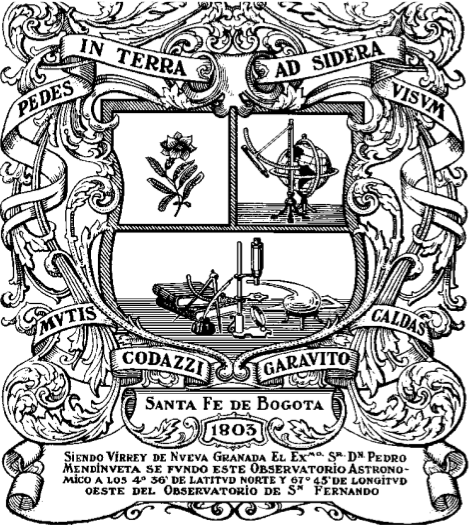
\includegraphics[width=0.35\textwidth]{imagenes/oan.png}
\end{center}

\renewcommand\contentsname{Contenido} 
\clearpage
\tableofcontents
\setcounter{page}{3}
\newpage

%
\pagestyle{fancy}
\chapter*{Introducci\'on}
\addcontentsline{toc}{chapter}{Introducci\'on}
%\mark{Introducci\'on}

\section*{El Sol}
\addcontentsline{toc}{section}{El Sol}

\vspace{0.2 cm}
{\renewcommand{\baselinestretch}{1.5}
{\footnotesize
\begin{flushright}
\begin{minipage}[h]{6cm}
\raggedleft{{\it solo es una bola de gas incandescente\\... cierto?}}
\end{minipage}
\end{flushright}}
\vspace{0.5cm}

\selectlanguage{spanish}

\noindent El Sol es la estrella m\'as cercana a nosotros (la siguiente est\'a unas 268 000 veces m\'as lejos) y por lo tanto es el objeto astron\'omico que con mayor intensidad influye en nuestro  vivir  cotidiano y en la curiosidad humana. Cuando se escudri\~na en el registro hist\'orico de las  civilizaciones antiguas se encuentra que, desde \'epocas remotas, el Sol ha tomado un papel de  importancia relevante en las visiones cosmol\'ogicas y cosmog\'onicas de distintas sociedades para el entendimiento del mundo \citep[]{vazquez2006}.\\

Aunque la naturaleza de nuestra estrella hu\'esped  y su relaci\'on con el sostenimiento de la vida en nuestro planeta ha inquietado al hombre durante varias generaciones, solo hasta comienzos del siglo XVII fue cuando se inici\'o un estudio riguroso y sistem\'atico del mismo. Este nacimiento de la f\'isica solar, por decirlo de alguna manera, fue desencadenado en gran medida gracias a las observaciones de manchas oscuras en el Sol (hoy d\'ia conocidas como {\it manchas solares}�); por parte de {\it Johannes Fabricius}, {\it Cristoph Schreiner} y {\it Galileo Galilei} de forma independiente; que rompieron con la concepci\'on equivocada de un Sol apol\'ineo e inalterable y que dieron pie al nacimiento de una ciencia que se encargara de estudiar su din\'amica.\\

El Sol es el objeto central de nuestro sistema solar y contiene un $99.8\%$ de la masa total del sistema. El Sol en s\'i mismo es una estrella que orbita el centro de nuestra galaxia, la {\it V\'ia L\'actea}, con una velocidad de unos $217\, \text{km/s}$ y un periodo de revoluci\'on de unos 230 millones de a\~nos (la \'ultima vez que el Sol estuvo en esta parte de la galaxia fue cuando aparecieron los dinosaurios). Comparado con la poblaci\'on de estrellas en nuestra galaxia, el Sol es una estrella com\'un que tiene un tama\~no medio y se encuentra en la mitad de su vida activa. En lenguaje astrof\'isico, es una estrella de tipo espectral G2 y de clase V en luminosidad, localizada en la secuencia principal del diagrama Hertzprung-Russell. De acuerdo con los modelos, el Sol ha permanecido en la secuencia principal por cerca de unos 5 000 millones de a\~nos y le restan otros 5 000 millones de a\~nos antes de que pase a la fase de las gigantes.\\

Uno de los encantos que tiene el estudiar el Sol hoy en d\'ia es que es aquella estrella de la que obtenemos la mayor cantidad de energ\'ia, suficiente como para estudiar su espectro en gran detalle y manejar una cadencia temporal muy peque\~na. Con m\'etodos indirectos es posible generar im\'agenes de la estructura superficial de otras estrellas cercanas. Pero con el Sol la historia es diferente; usando telescopios y t\'ecnicas comunes de la astronom\'ia es posible resolver estructuras por debajo de los 700 km de tama\~no  en su superficie, que representa la resoluci\'on espacial l\'imite con la que se trabaja en la presente tesis. Por su extrema cercan\'ia, tambi\'en es comparativamente sencillo estudiar la estructura de su atm\'osfera y los efectos de origen magn\'etico que tienen lugar all\'i, como es el caso de las fulguraciones solares (fen\'omeno de mayor inter\'es en este trabajo), las eyecciones coronales de masa, las manchas solares, las f\'aculas, los agujeros coronales, las esp\'iculas, {\it plages}, entre otros.\\

\renewcommand{\baselinestretch}{1.0}

\begin{wrapfigure}[15]{r}{0.41\textwidth}
\begin{center}
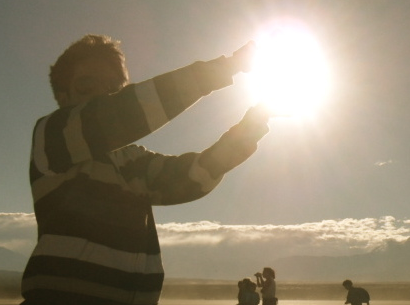
\includegraphics[width=0.32\textwidth]{Sun_in_hands.png}
\caption{El tama\~no aparente del Sol sobre nuestro cielo es de unos $\sim 32$ minutos de arco, un poco m\'as grande que medio grado.}
\label{solar-size}
\end{center}
\end{wrapfigure}

El Sol es el objeto m\'as brillante en nuestro cielo; es 12 magnitudes m\'as brillante que el segundo objeto m\'as brillante de una noche despejada y clara, la Luna llena. Su radiaci\'on es la responsable del calentamiento lum\'inico de la superficie terrestre, y por tanto un factor determinante del clima y en la sostenibilidad de la vida. El viento solar es quien nos separa del medio interestelar impidiendo que una gran cantidad de part\'iculas penetren nuestro sistema solar y puedan generarnos alg\'un da\~no. El campo magn\'etico solar nos protege de la incidencia de rayos c\'osmicos muy energ\'eticos, pero a su vez eventos muy violentos de origen magn\'etico que tengan lugar en su superficie podr\'ian alterar considerablemente nuestros sistemas de comunicaciones en tierra.\\

El Sol posee una estructura compleja. Esencialmente, este puede ser descrito como un conglomerado gigante de Hidr\'ogeno y Helio con un peque\~no porcentaje de elementos pesados aproximadamente en una relaci\'on de masa en su superficie de $\sim73.46\%$, $\sim24.85\%$ y $\sim1.69\%$ en masa, respectivamente. Debido a su gran masa la auto-gravitaci\'on mantiene a la estructura en forma de esfera casi completamente perfecta. El peso de las capas exteriores de gas incrementan la presi\'on en las regiones internas del Sol y dan lugar a los fen\'omensos de fusi\'on termonuclear que mantienen a la estrella en un constante equilibrio hidrost\'atico.


\subsection*{Estructura Interna}
\addcontentsline{toc}{section}{Estructura Interna}

 En el n\'ucleo solar la densidad, la presi\'on y la temperatura son tan altas del orden de 150 g/cm$^3$, $2.5\times 10^{17}$ din/cm$^3$ y 13 millones de kelvin respectivamente, que forman el ambiente propicio para que tengan lugar reacciones de fusi\'on termonuclear cuyo proceso principal es la quema de Hidr\'ogeno en Helio. Como resultado de este proceso, se tiene la producci\'on de energ\'ia en forma de radiaci\'on electromagn\'etica que involucra fotones de muy altas frecuencias y una alta emisi\'on de neutrinos. Debido a la alta densidad del medio, dichos fotones son continuamente absorbidos y re-emitidos por los iones cercanos, de manera que esa gran cantidad de energ\'ia producida en el interior es suave y lentamente radiada hacia el exterior de la estrella. Seg\'un esto, los fotones que hoy est\'an alcanzando la superficie de la tierra fueron generados en el interior solar apenas cuando el {\it Homo Sapiens} estaba apareciendo, o sea hace unos 170 000 a\~nos \citep[]{mitalas1992}.\\

\begin{SCfigure}
\centering
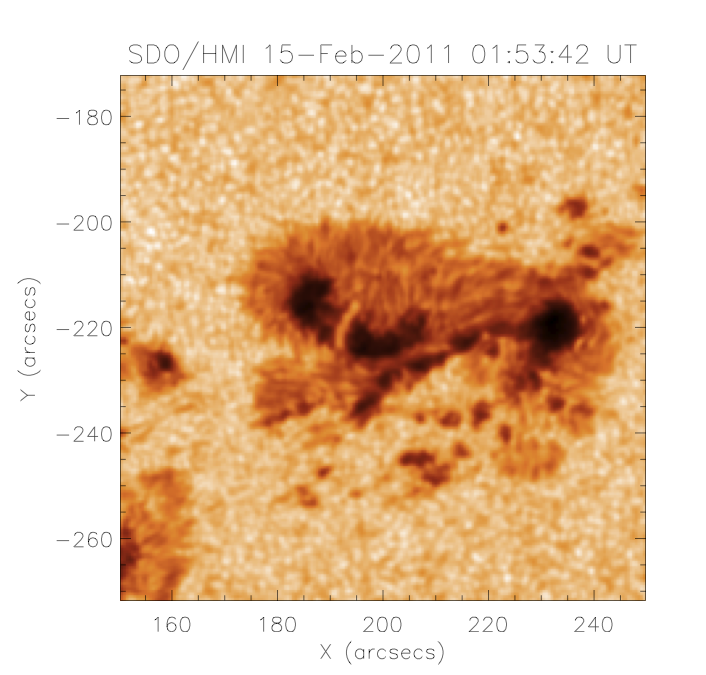
\includegraphics[width=0.63\textwidth]{resolution.png}
\caption{Regi\'on activa SOL2011-02-15T01:52 X2.2 registrada por SDO/HMI. Imagen de la ``superficie'' solar (fotosfera) con una resoluci\'on de $\sim 100$ km. Los gr\'anulos se ven en todas partes como peque\~nas zonas claras rodeadas por regiones oscuras. Sus formas se deben a que conforman la parte alta de la zona convectiva donde la energ\'ia se transporta desde el interior v\'ia el movimiento del gas. En la superficie el gas se enfria debido a que la energ\'ia se radia hacia el exterior. Las l\'ineas de campo magn\'etico fuertemente localizadas son las responsables de generar las zonas oscuras que se ven (manchas solares) como consecuencia de un decremento en la eficiencia del transporte radiativo en dicho lugar.}
\label{solar-size}
\end{SCfigure}

Aproximadamente a 0.7 radios solares del centro el mecanismo de transporte energ\'etico por {\it radiaci\'on} deja de ser eficiente. En ese lugar el gas se calienta, se expande, se vuelve din\'amico y se eleva hasta la superficie solar creando lo que se conoce como {\it celdas convectivas} que se encargan de transportar el gas caliente hasta la superficie donde se enfr\'ian y caen nuevamente para ser calentados y repetir el proceso una vez m\'as. Este flujo de gas transporta la energ\'ia hacia la parte externa del Sol donde la temperatura se reduce a unos $\sim 5\,700$ K y la densidad es lo suficientemente baja como para que los fotones puedan escapar de all\'i relativamente f\'acil, es decir, sin demasiadas interacciones con el plasma circundante. La regi\'on externa de donde recibimos la mayor cantidad de fotones \'opticos es com\'unmente llamada la {\it superficie solar} o {\it fotosfera} (esfera de luz), aunque no sea una capa s\'olida propiamente dicha.\\

La mayor\'ia de los fotones que recibimos provienen de all\'i y se encuentran en la regi\'on visible del espectro electromagn\'etico. Esta es muy probablemente la raz\'on por la que los seres vivos, en sus procesos de evoluci\'on pasados, desarrollaron \'organos de visi\'on que son mayormente sensibles en esta parte del espectro. Hacia afuera de esta capa se extiende radialmente la atm\'osfera solar, con un decremento de la densidad. Esta transici\'on ocurre acompa\~nada de un aumento en la temperatura que a\'un no est\'a completamente entendido y que alcanza unos cuantos millones de Kelvin. Por lo tanto debe existir una capa que tenga una temperatura m\'inima. Los modelos est\'andar proponen que esta capa se encuentra a una altura promedio de 500 km sobre la fotosfera y suponen una temperatura muy cercana a los 4000 K, suficientemente baja como para permitir la formaci\'on de mol\'eculas tales como el CO y/o el vapor de agua. A los dos lados de esta capa la temperatura se incrementa. Tambi\'en, en los modelos est\'andar, se considera que la capa posterior a esta se extiende unos 1 500 km hacia el exterior y alcanza temperaturas de los 8 000 a 10 000 K. Esta capa se conoce como la {\it cromosfera}. Enseguida a ella se encuentra la {\it regi\'on de transici\'on} donde la temperatura se incrementa abruptamente. Finalmente se tiene la parte m\'as externa de la atm\'osfera solar, llamada la {\it corona}, donde permanentemente se presenta un flujo continuo de part\'iculas que se mueve a lo largo de las l\'ineas de campo magn\'etico y conforma el {\it viento solar}. Dicho viento solar se extiende unas 100 000 veces el radio solar, mucho m\'as all\'a de \'orbita de Plut\'on, hasta la frontera de nuestro sistema solar, la {\it heliopausa}. Su interacci\'on con el medio interestelar crea un frente de choque, que est\'a siendo medido desde el 2009 por las sondas espaciales Voyager 1 y Voyager 2.\\

\renewcommand{\baselinestretch}{1.0}

\begin{wrapfigure}[29]{r}{0.58\textwidth}
\begin{center}
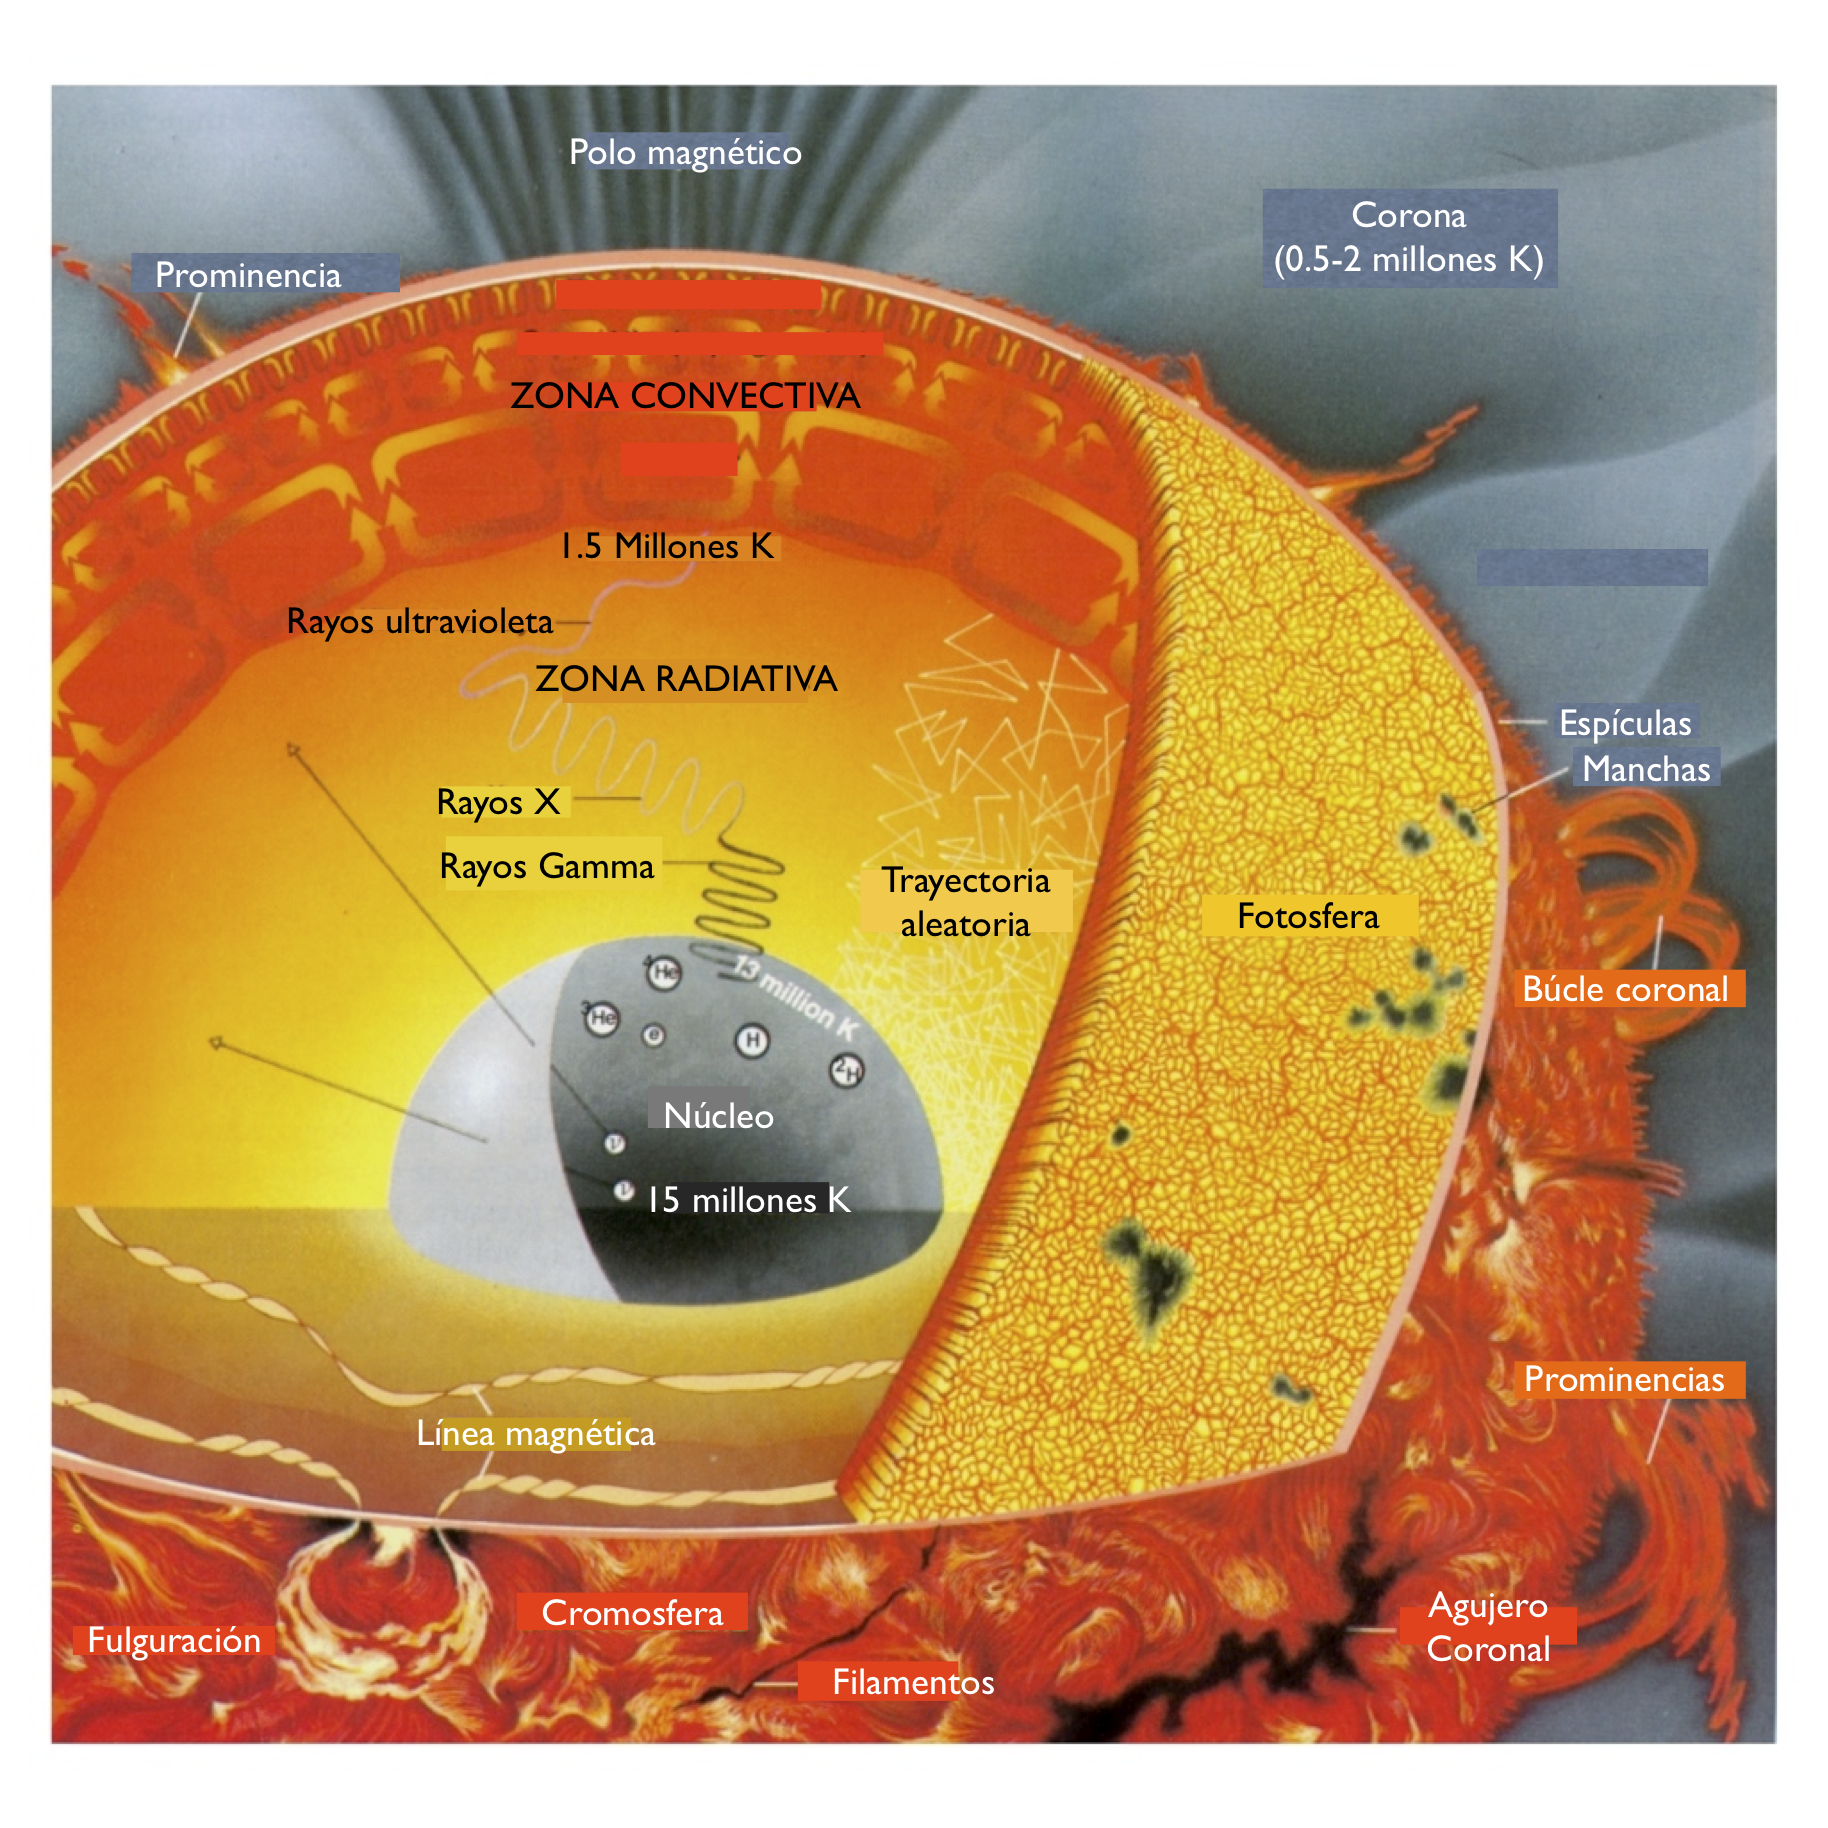
\includegraphics[width=0.58\textwidth]{sun.png}
\caption{Esquema de la estructura interna del Sol. Tres grandes zonas interiores en donde se genera y transporta la energ\'ia. Muchos fen\'omenos superficiales de origen magn\'etico.}
\label{sol}
\end{center}
\end{wrapfigure}

Detr\'as de esta estructura de capas, el Sol resulta ser a\'un m\'as complejo. Algunas otras propiedades que podemos describir brevemente, son:\\

- El Sol vibra. Considerado como una esfera auto-gravitante, compresible y en equilibrio, el Sol puede vibrar. Las perturbaciones en presi\'on y densidad generadas principalmente por las fluctuaciones convectivas se pueden propagar a lo largo de toda la estructura solar. Aquellas ondas con frecuencias cercanas entre s\'i pueden generar muchos modos normales de oscilaci\'on que sobre la superficie solar son vistas como patrones caracter\'isticos de diferentes configuraciones de interferencia constructiva. Estas vibraciones de baja amplitud (apenas unos cuantos cientos de metros por segundo en la fotosfera) pueden ser medidas y descompuestas en {\it modos propios} de oscilaci\'on mediante t\'ecnicas que involucran un an\'alisis por corrimiento Doppler y largos periodos de observaci\'on. La propagaci\'on de las ondas depende de las propiedades del medio. Es posible entonces suponer el camino contrario, mediante la medida de los patrones de vibraci\'on conocer algunas caracter\'isticas del medio propagador. Algunas ondas se propagan \'unicamente cerca de la superficie solar, pero otras, en cambio, pueden sumergirse completamente hasta el interior de la estructura. Estas \'ultimas ondas de las que se habla son la principal fuente de informaci\'on para inferir propiedades de estructura tales como la temperatura, densidad y presi\'on que puedan servir de {\it test} para evaluar la validez o no de un cierto modelo solar. De esto es justamente de lo que se encarga la {\it heliosismolog\'ia global} quien mediante los patrones de vibraci\'on determina diferentes valores de las propiedades globales de estructura. La {\it heliosismolog\'ia local} describe la din\'amica de los alrededores de una cierta perturbaci\'on que se da a nivel local, usualmente sobre la superficie del Sol (como es el caso de los fen\'omenos que se estudian en esta tesis).\\

- El Sol rota. La conservaci\'on del momentum angular de una nube de gas y polvo rotante puede dar pie al nacimiento de una estrella que despu\'es de contraerse rota a\'un m\'as r\'apido. Es ampliamente aceptado que el momentum angular de nuestra estrella fue removido durante sus primeras fases de vida por un fuerte campo magn\'etico anclado al medio interestelar circundante y por un viento fuerte. El remanente de dicho momentum angular inicial es el que vemos hoy en el Sol. El Sol no es un cuerpo r\'igido de manera que su periodo de rotaci\'on var\'ia con la latitud helioc\'entrica y con la distancia radial a su n\'ucleo. Hacia la zona equatorial el periodo sin\'odico de rotaci\'on en la superficie es de 27.2753 d\'ias, mientras que en los polos es de aproximadamente de 32 d\'ias. Mediante an\'alisis heliosismol\'ogicos se han encontrado registros de una rotaci\'on diferencial pero continua hasta una cierta profundidad (0.7 $R_\odot$), la {\it tacoclina}, a partir de la cual la rotaci\'on del Sol es como la de un cuerpo r\'igido que mantiene un periodo de rotaci\'on como el de las latitudes medias en la superficie. La rotaci\'on diferencial genera un flujo meridional de gas que va directamente a los polos cerca de la superficie y hacia el ecuador en la base de la zona convectiva.\\


\begin{figure}
\centering
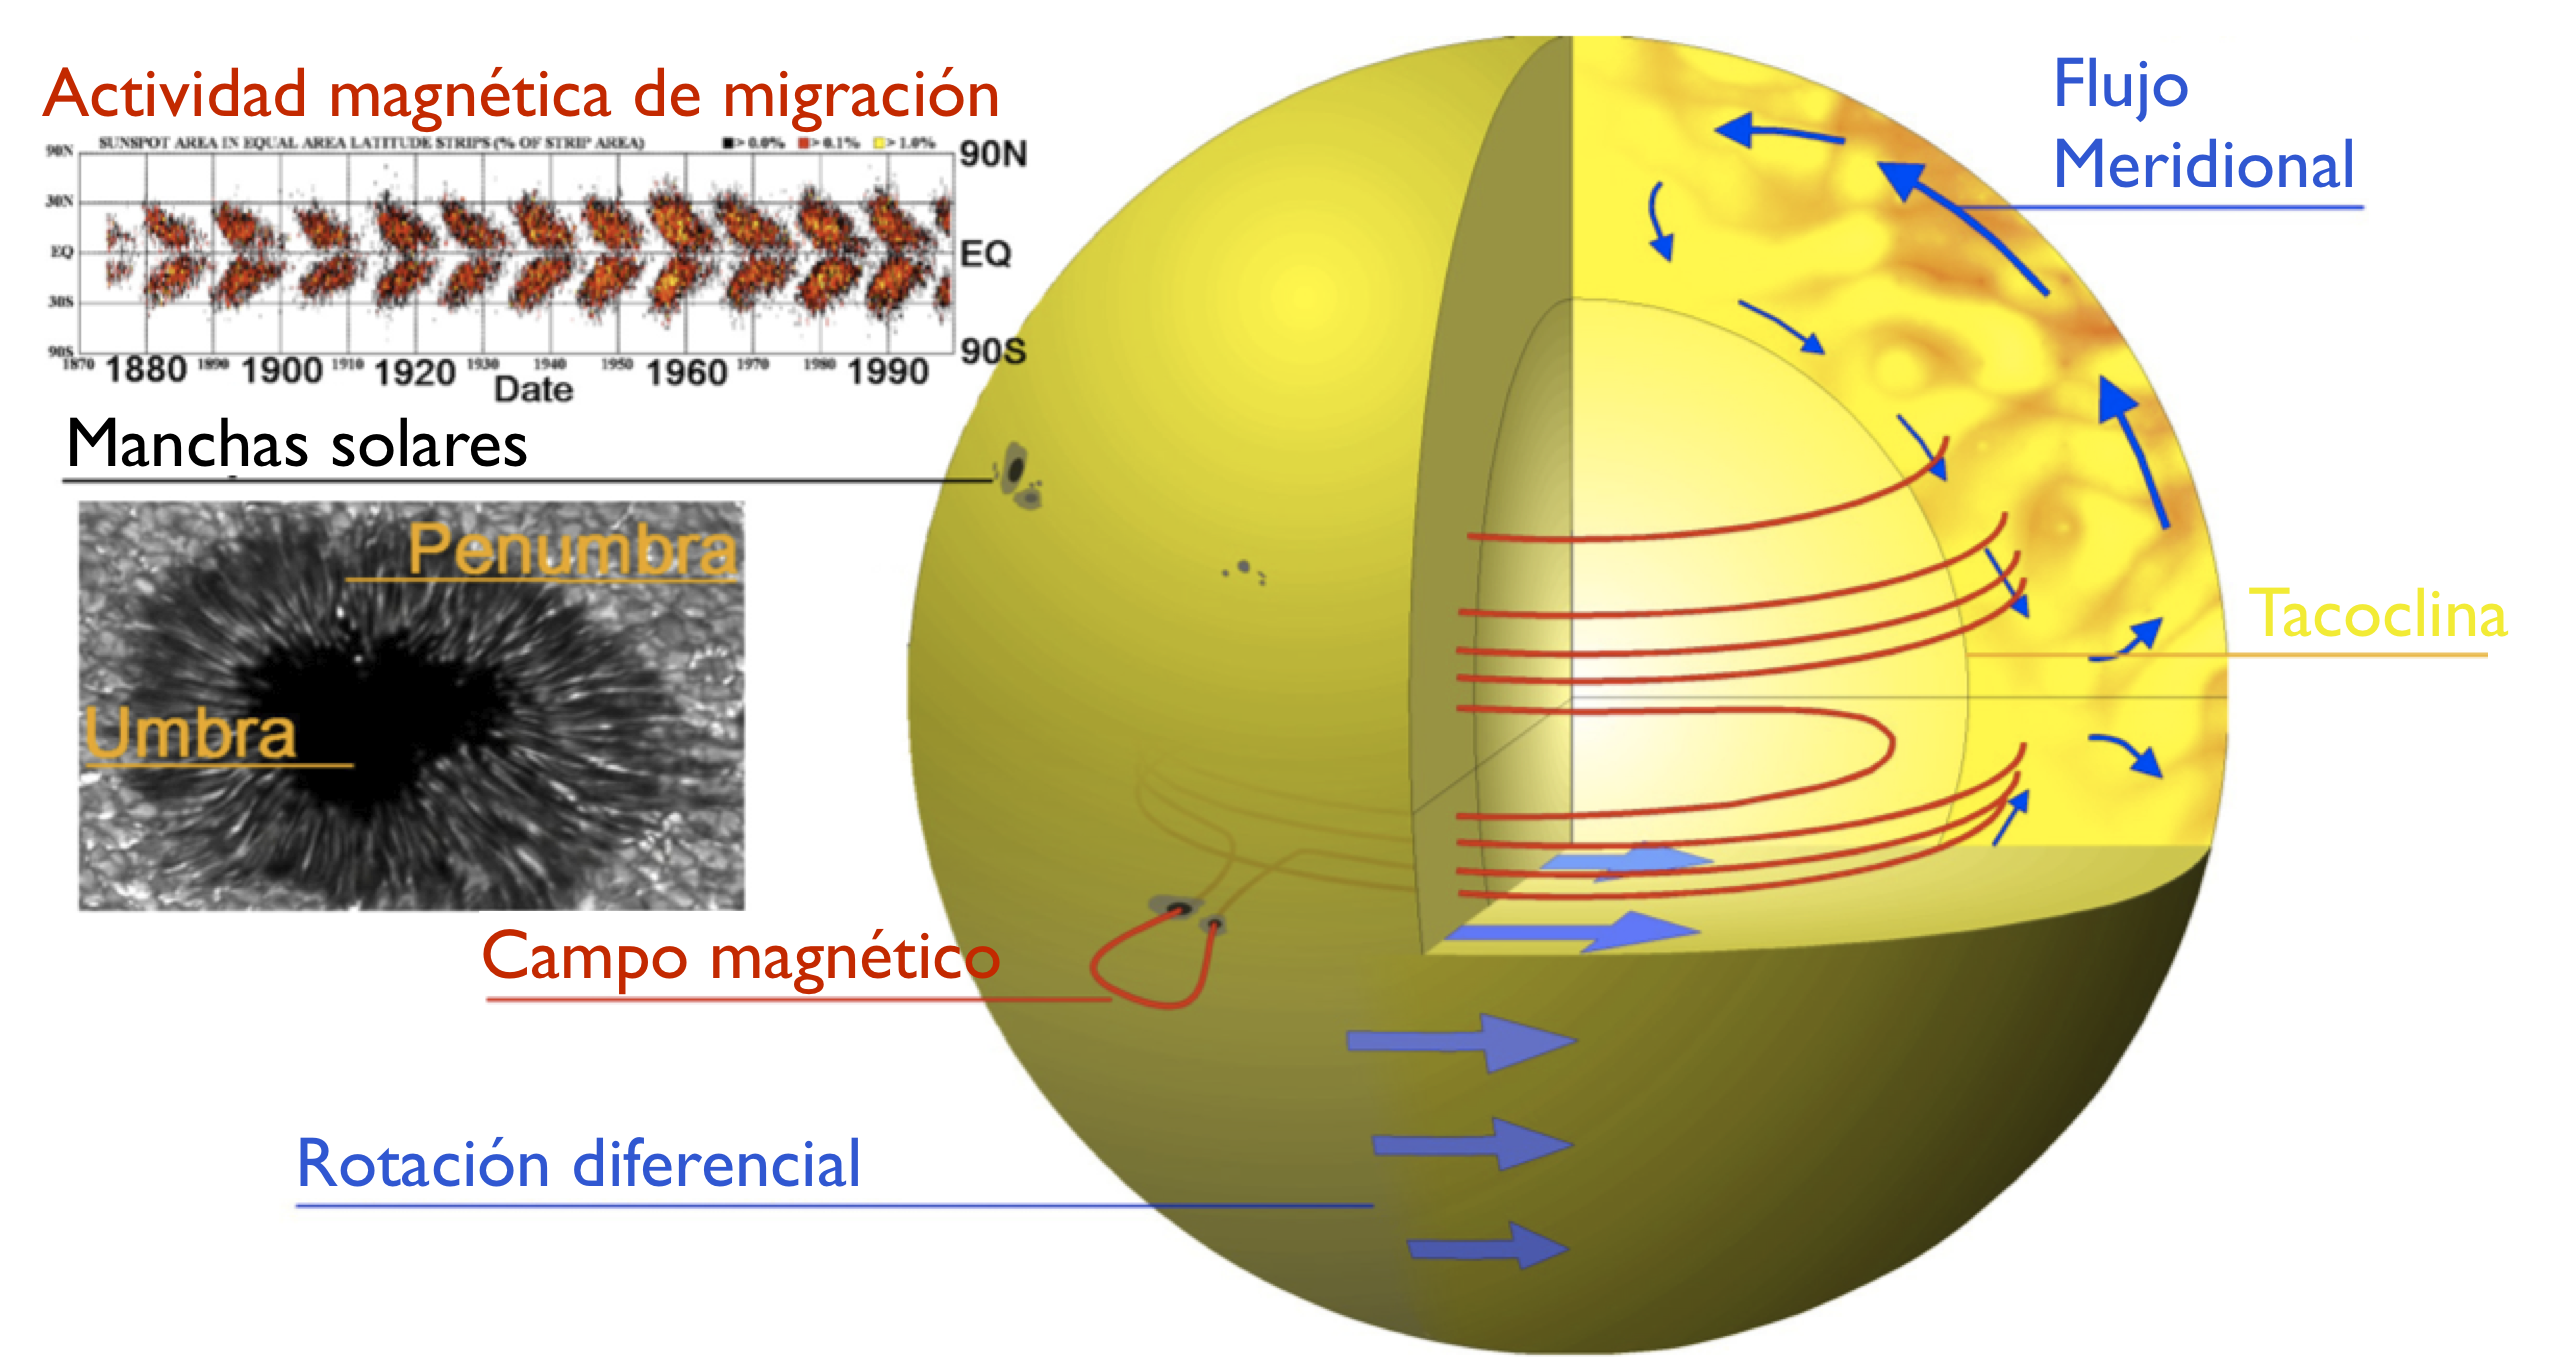
\includegraphics[width=1.0\textwidth]{sun_parts.png}
\caption{Representaci\'on gr\'afica de los diferentes aspectos del ciclo de actividad solar: Las l\'ineas de campo magn\'etico (rojas) se acumulan por la convecci\'on y la rotaci\'on diferencial (azul). El flujo meridional (azul), transporta la energ\'ia magn\'etica hacia el ecuador. En aquellas partes donde l\'ineas fuertes de campo magn\'etico penetren la fotosfera son generadas las manchas solares. Al inicio del ciclo solar las manchas aparecen en regiones de latitudes altas y a medida que transcurre el tiempo su aparici\'on se va desplazando hacia la zona ecuatorial. Referencia: Esta imagen fue tomada y modificada de \citep[]{kneer2003}}
\label{solar}
\end{figure}

- El Sol muestra una (compleja) actividad magn\'etica. El Sol posee una topolog\'ia de campo magn\'etico que macrosc\'opicamente mantiene una configuraci\'on dipolar d\'ebil. Sin embargo, la superficie solar puede albergar fen\'omenos que involucran muy fuertes y complicadas estructuras magn\'eticas observadas a trav\'es de su manifestaci\'on con las extra\~nas formas y din\'amicas que adopta el plasma superficial e.g. la baja eficiencia en el transporte energ\'etico que conduce a la aparici\'on de {\it manchas solares}. Toda la materia en el Sol se encuentra en forma de plasma debido a las temperaturas muy altas que se manejan all\'i. La alta conductividad que tienen las part\'iculas cargadas propias de un plasma hacen que despu\'es de que se ha alcanzado un cierto grado de equilibrio se genere un congelamiento de las l\'ineas de campo en \'el. La fuente de estas bien localizadas y fuertes l\'ineas de campo es a\'un hoy en d\'ia desconocido. Las teor\'ias de d\'inamo direccionan este problema sugiriendo que el campo magn\'etico dipolar d\'ebil es amplificado hacia la base de la zona convectiva por un movimiento estoc\'astico de la masa y retorcido producto de la convecci\'on y de la rotaci\'on diferencial.\\

- El Sol tiene ciclos. El Sol sufre fluctuaciones en el tiempo. Estos cambios se ven reflejados en la irradiancia total, en el viento solar y el campo magn\'etico. Esto sucede en un ciclo aproximadamente regular, como el ciclo de 11 a\~nos de las manchas solares, pero con aperidicidades en escalas extendidas de tiempo, como es el caso del m\'inimo de Mounder (un periodo de 75 a\~nos en el siglo XVII donde las manchas solares tuvieron un comportamiento extra\~no y que coincidi\'o con la llamada {\it peque\~na era de hielo}). Estas fluctuaciones modulan la estructura de la atm\'osfera solar, corona y viento solar, la irradiancia total, la aparici\'on de fulguraciones y eyecciones coronales de masa y tambi\'en indirectamente la incidencia en tierra o no de rayos c\'osmicos de fondo altamente energ\'eticos. Ninguna de estas variaciones ha sido completamente entendida y los efectos que desde el Sol se desprenden hacia la tierra a\'un son cuesti\'on de debate. La idea m\'as generalmente aceptada sobre los ciclos y fluctuaciones aperi\'odicas es que son causadas por cambios en la configuraci\'on del campo magn\'etico, frecuentemente entendidos y modelados mediante los mecanismos d\'inamo.\\

- El Sol evoluciona. Nuestra estrella se encuentra en este momento en la fase de la {\it secuencia principal}, donde la mayor fuente de energ\'ia es la fusi\'on nuclear de Hidr\'ogeno a Helio. Despu\'es de la fase inicial de acreci\'on de masa vino una fase entera de auto-gravitaci\'on en la que ha permanecido y permanecer\'a la mayor parte de su vida. En el caso del Sol, a\'un le restan otros cinco mil millones de a\~nos antes de que pase a un estado de evoluci\'on posterior que incluye una variaci\'on compleja en su radio y la quema de Helio como fuente de energ\'ia en su fase final de gigante roja. Al final de su vida, se cree que, terminar\'a como una {\it enana blanca}.\\

Dado que el tema que aqu\'i se plantea abordar involucra el entendimiento en m\'as detalle de las fulguraciones solares y de la heliosismolog\'ia local, son temas en los que se profundiza a continuaci\'on. Los lectores que est\'en interesados en encontrar m\'as informaci\'on general acerca del Sol pueden encontrarla en \citep[]{vaquero2009} y en las diferentes referencias que se citan all\'i.

\section*{Fulguraciones solares y otros eventos explosivos}
\addcontentsline{toc}{section}{Fulguraciones solares y otros eventos explosivos}

Una de las m\'as grandes diferencias entre los astrof\'isicos y los f\'isicos de otras \'areas es que los primeros no pueden reproducir ni analizar sus objetos de investigaci\'on en un laboratorio. Los astrof\'isicos dependen de lo que puedan obtener de sus observaciones. Part\'iculas que llegan de todas partes del universo son las mensajeras que traen informaci\'on de objetos muy distantes a nosotros. Naturalmente, muchas veces, esta informaci\'on puede ser muy dif\'icil de obtener o insuficiente. En este contexto los f\'isicos solares corren con una apreciable ventaja ya que su objeto de estudio es el m\'as cercano a nosotros en todo el universo. El Sol es la \'unica estrella de la que hoy es posible resolver espacialmente y en detalle su superficie mediante observaciones directas, permitiendo el estudio fino de estructuras cuya escala sea apenas de unos cuantos cientos de kil\'ometros. Adem\'as, es un objeto que est\'a siendo monitoreado permanentemente usando tanto estaciones en tierra como instrumentos espaciales que liberan miles de gigabytes al d\'ia. Aunque por razones evidentes no podamos variar los par\'ametros f\'isicos en este ``laboratorio'', s\'i podemos estudiar fen\'omenos extravagantes, que son imposibles de reproducir en tierra pero, que tienen lugar en todas partes del universo. Un ejemplo, que nos ata\~ne, de estos son las {\it fulguraciones solares}.\\

Entre los varios fen\'omenos que involucran una fuerte actividad magn\'etica en el Sol, las fulguraciones solares son particularmente fascinantes por la enorme potencia con la que se presentan. En una fulguraci\'on corriente se puede liberar una cantidad de energ\'ia del orden de $10^{32}$ erg ($10^{25}$ Joules) en unos cuantos segundos o minutos. Si por ejemplo se considera una fulguraci\'on cuya duraci\'on es de 10 minutos, su potencia puede ser estimada es unos $1.7\times10^{22}$ W que resulta ser unas 200 000 veces el consumo total de energ\'ia mundial durante el 2006 ($5\times10^{20}$ J) \citep[]{energy2006}. Se cree que dicha energ\'ia tiene un origen magn\'etico, y que es liberada cuando las l\'ineas de campo magn\'etico se reconectan en la corona. En estos procesos, las part\'iculas circundantes son aceleradas a altas energ\'ias y  liberadas hacia el espacio interplanetario a lo largo de las l\'ineas ``abiertas'' de campo o precipitadas hacia la cromosfera a trav\'es de las l\'ineas de campo del nuevo bucle reconectado. La interacci\'on colisional con el plasma de los alrededores produce una desaceleraci\'on o frenado completo del jet de part\'iculas emitiendo radiaci\'on bremsstrahlung (interacci\'on libre-libre) que puede ser observada en rayos-X (en este contexto tambi\'en llamados {\it footpoints}). El plasma cromosf\'erico se expande como producto del calentamiento producido por este tipo de interacciones, de manera que siendo menos denso sube a trav\'es de las l\'ineas de campo reconectadas estructurando la forma de bucle que vemos en rayos-X blandos o en EUV en este tipo de procesos. Esta din\'amica se conoce con el nombre de {\it evaporaci\'on cromosf\'erica}.\\

Los fen\'omenos m\'as explosivos de este tipo de eventos se observaron en la era moderna hacia finales de Octubre y comienzos de Noviembre de 2003. Para entonces, los sat\'elites con fines de telecomunicaci\'on geo-orbitantes tuvieron que apagarse temporalmente. Los astronautas en la {\it Estaci\'on Espacial Internacional} fueron forzados a permanecer en sus m\'odulos de servicio por un par de horas. Las aeronaves comerciales desviaron las rutas que pasaban por latitudes terrestres muy altas y en Suecia el suministro de corriente el\'ectrica colaps\'o dejando a cerca de 50 000 personas en oscuridad temporal. Estos eventos ayudan a mostrar la importancia que tiene la relaci\'on Sol-Tierra para la civilizaciones humanas modernas \citep[]{schwenn2006}.\\

Una fulguraci\'on en el Sol se define como un incremento espont\'aneo y r\'apido en la emisi\'on de radiaci\'on, en todo el rango del espectro electromagn\'etico (desde el radio hasta los rayos-$\gamma$), de alg\'un lugar bien localizado de la atm\'osfera solar. Este puede estar acompa\~nado de un calentamiento del plasma local, y un movimiento brusco de masa (por ejemplo una eyecci\'on coronal de masa). En fracci\'on de segundos una gran cantidad de la energ\'ia de la fulguraci\'on es transferida  a la aceleraci\'on de part\'iculas (principalmente, pero no exclusivamente, electrones). 

\begin{figure}
\centering
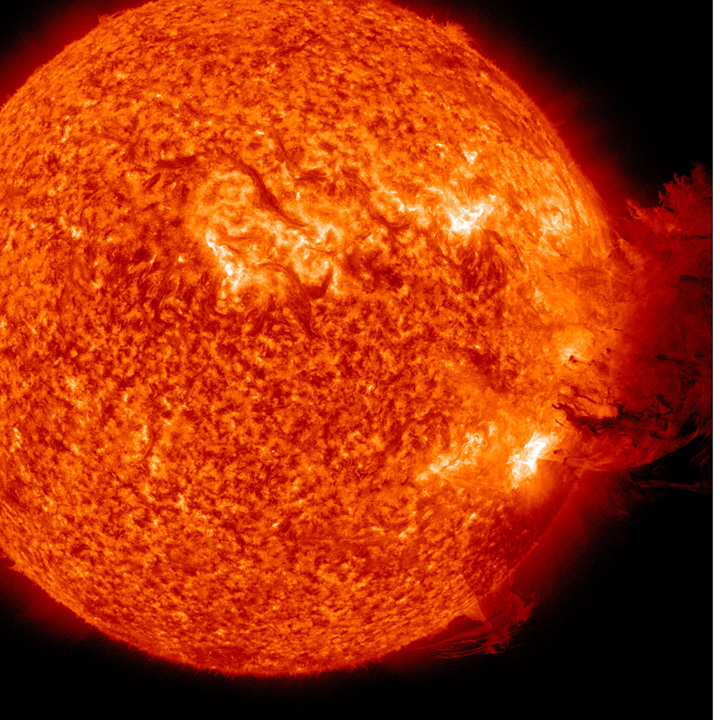
\includegraphics[width=0.99\textwidth]{sdoflare.jpg}
\caption{Fulguraci\'on tipo M2 (de tama\~no medio) junto con una eyecci\'on coronal de masa que ocurri\'o el pasado 7 de Junio de 2011 a las 01:41 TU. Tomada en EUV por SDO/AIA a 304\AA. La CME ten\'ia rumbo hacia la tierra con una velocidad de $\sim1 400$ km/s. Los efectos sobre la tierra fueron muy leves, apenas unas cuantas auroras. Imagen tomada de: sdo.gsfc.nasa.gov/gallery.}
\label{sdoflare}
\end{figure}

\subsection*{Fases de las fulguraciones solares}
\addcontentsline{toc}{subsection}{Fases de las fulguraciones solares}

Como se mencion\'o anteriormente, las fulguraciones solares emiten en un amplio rango del espectro electromagn\'etico. La intensidad de emisi\'on y la forma que toma la curva de luz para cada valor de frecuencia est\'an directamente asociadas a una variedad de diferentes procesos f\'isicos que se presentan seg\'un la din\'amica del fen\'omeno. Varios trabajos se han desarrollado en torno a la caracterizaci\'on de estos espetros y curvas de luz en busca de definir una especie de ``taxonom\'ia'' que permita distinguir las diferentes fases por las que tiene que pasar una fulguraci\'on \citep[]{mo2009,fletcher2011}.

\subsubsection*{Pre-fulguraci\'on}
\addcontentsline{toc}{subsubsection}{Pre-fulguraci\'on}

En esta fase la energ\'ia magn\'etica se acumula lentamente en la corona solar. Este proceso puede durar de entre unas cuantas horas a un par de d\'ias. Por medio de alg\'un mecanismo, que a\'un es tema de discusi\'on, la configuraci\'on de campo magn\'etico se desestabiliza y la energ\'ia es liberada espont\'aneamente. A esta antesala de la fulguraci\'on se le conoce tambi\'en como la {\it fase  precursora}. El aumento en la emisi\'on de radiaci\'on a diferentes frecuencias no necesariamente se presenta en el lugar de la explosi\'on, y depende de las propiedades f\'isicas que acompa\~nan al proceso. A partir de estas, se ha catalogado esta fase seg\'un las observaciones que se han obtenido. Estas clases son:\\

{\it - Fulguraciones hom\'ologas}. En algunas ocasiones las regiones activas presentan fulguraciones de baja intensidad y en movimiento que tienen lugar antes y muy cerca de la fulguraci\'on principal. Este fen\'omeno muestra que el campo magn\'etico, y en particular el torcimiento de las l\'ineas, tiene una din\'amica que lo hace cambiar en el tiempo. Tales cambios podr\'ian, eventualmente, generar el desencadenamiento de la gran explosi\'on.\\


{\it - Fulguraciones sympathetic}. Este tipo de eventos han sido observados en regiones magn\'eticas del Sol que se relacionan de manera cercana. Un ejemplo t\'ipico es la observaci\'on de fulguraciones casi completamente sincronizadas que ocurren en diferentes regiones del disco solar. Este fen\'omeno resulta ser muy llamativo ya que muestra fulguraciones ocurriendo en diferentes lugares que, en principio, podr\'ian ser transmitidas a otras zonas en donde eventualmente inducir\'ian fulguraciones mucho mayores.\\

{\it - Rayos-X blandos precursores}. Algunas veces es posible observar rayos-X blandos transitorios que pueden durar hasta unas cuantas decenas de minutos. En esta configuraci\'on, la distribuci\'on del campo magn\'etico en la corona es complicada y est\'a compuesta de muchos grandes y peque\~nos bucles. Algunas veces estos peque\~nos bucles interact\'uan con el bucle principal de la regi\'on activa. Esta interacci\'on, cuando se presenta, puede generar peque\~nas fulguraciones que pueden ser vistas en rayos-X blandos debido a la radiaci\'on t\'ermica que all\'i se presenta, pero quiz\'as lo m\'as importante de esta din\'amica es que esta interacci\'on puede llevar a contribuir a la desestabilizaci\'on del campo magn\'etico e inducir una fulguraci\'on a\'un m\'as grande.\\

{\it - Radiaci\'on precursora en radio}. Como se mencion\'o anteriormente, las fulguraciones solares radian en una amplia regi\'on del espectro electromagn\'etico. La radiaci\'on precursora en radio es un cambio en la intensidad y/o la polarizaci\'on de la radiaci\'on emitida en este rango del espectro por parte de la regi\'on activa observada sobre todo en microondas con una duraci\'on t\'ipica de las decenas de minutos.\\


{\it - Precursores en extremo ultra-violeta (EUV)}. Es el caso en el que se ve un acrecentamiento de la emis\'on en EUV en peque\~nos n\'ucleos localizados que despu\'es pueden ser correlacionados con la presencia de la fulguraci\'on. Tanto en este caso como en los precursores de radio las emisiones son asociadas con la reconfiguraci\'on de las l\'ineas de campo magn\'etico.\\


Frecuentemente estos {\it precursores} resultan ser indicadores directos o indirectos de la evoluci\'on del campo magn\'etico en regiones fulgurantes. Sin embargo, para estudiar los cambios reales del campo magn\'etico es necesario medirlo tanto en la corona sola como en la fotosfera. Varias t\'ecnicas son usadas con tal fin. Una de ellas hace uso de los magnetogramas vectoriales en busca de interpolar el campo magn\'etico en la corona y determinar su valor \citep[]{wheatland2000,wang2011}. En otras, se hace uso de las observaciones en radio de regiones {\it cuasi-transversales} donde es posible deducir el valor de campo magn\'etico en la corona \citep{Ryabov2005}. 

\subsubsection*{Fase impulsiva}
\addcontentsline{toc}{subsubsection}{Fase impulsiva}

Una de las formas m\'as sencillas de considerar una fulguraci\'on es la siguiente: Despu\'es de que la energ\'ia magn\'etica es almacenada durante la fase de la prefulguraci\'on se libera por alg\'un mecanismo de desestibilizaci\'on del campo magn\'etico coronal. Como resultado, el plasma local se calienta y las part\'iculas son r\'apidamente aceleradas. Los haces de part\'iculas no t\'ermicas se propagan a lo largo de las l\'ineas de campo magn\'etico alcanzando, eventualmente, la cromosfera y la fotosfera solar. As\'i como algunas de las part\'iculas aceleradas son precipitadas hacia la atm\'osfera solar, otras pueden salir en direcci\'on contraria (incluso como cantidades grandes de masa) hacia el espacio interplanetario.\\

\renewcommand{\baselinestretch}{1.0}

\begin{wrapfigure}[35]{r}{0.49\textwidth}
\begin{center}
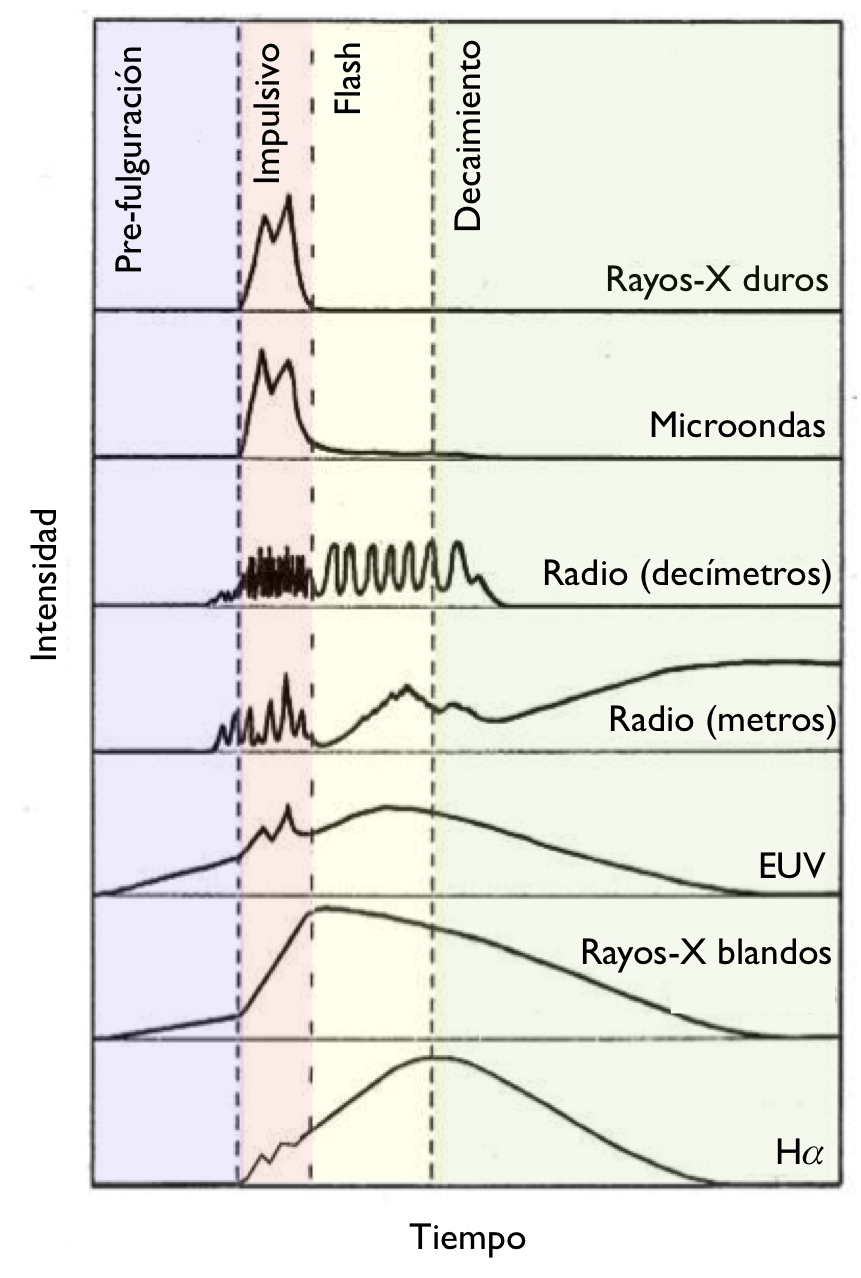
\includegraphics[width=0.49\textwidth]{lo.png}
\caption{Esquema general de los perfiles temporales de la emisi\'on en diferentes rangos del espectro electromagn\'etico de una fulguraci\'on solar. Figura tomada y adaptada de \citep[]{benz2002}.}
\label{sol}
\end{center}
\end{wrapfigure}

La fase impulsiva se caracteriza por un incremento r\'apido y brusco de la intensidad en todas las frecuencias. Varios estudios del perfil temporal del flujo en las fulguraciones solares han mostrado fluctuaciones que indican la presencia de un mecanismo impulsador que inyecta cierta cantidad de part\'iculas en el bucle \citep[]{aschwanden2004}. Durante esta fase es posible observar una gran variedad de tipos de radiaci\'on en diferentes lugares del arco magn\'etico. Estas emisiones, en particular en rayos-X y en radio, nos dan informaci\'on del mecanismo por el cual son aceleradas las part\'iculas y mediante el cual la liberaci\'on de energ\'ia tiene lugar durante esta fase impulsiva. Los rayos-X duros son producidos en la fotosfera en las bases del bucle (o los as\'i llamados {\it footpoints} en ingl\'es) v\'ia radiaci\'on de frenado, o {\it Bremsstrahlung}, por la colisi\'on del chorro de electrones con el ambiente cromosf\'erico denso (principalmente compuesto de iones). Cuando se habla de rayos-$\gamma$ casi siempre estos tienen un origen nuclear. As\'i, las l\'ineas observadas en este rango de frecuencias son debidas a la colisi\'on entre los protones acelerados en la fulguraci\'on y el plasma cromosf\'erico. La emisi\'on en {\it radio} es debida a otro mecanismo de radiaci\'on. Existen dos formas b\'asicas de producir un flujo neto en radio, por emisi\'on t\'ermica y no-t\'ermica. Este \'ultimo es debido a un efecto del movimiento de los electrones a lo largo de las l\'ineas de campo magn\'etico conocido como  radiaci\'on {\it giro-sincrotr\'on}. Se ha observado que el flujo en esta banda est\'a muy fuertemente correlacionado con la emisi\'on en rayos-X asociada a los {\it footpoints} en este tipo de eventos. Este hecho puede ser explicado si se supone que ambas poblaciones de electrones no-t\'ermicos, responsables de la emisi\'on en radio y en rayos-X duros, tienen un origen com\'un en la fulguraci\'on solar. La observaci\'on en {\it microondas} tiene una importancia bien particular, ya que se supone que esta emisi\'on se produce justo antes que las part\'iculas pierdan su energ\'ia v\'ia colisiones de forma que nos pueda brindar informaci\'on acerca del mecanismo por el cual fueron aceleradas dichas part\'iculas.

\subsubsection*{Fase del flash}
\addcontentsline{toc}{subsubsection}{Fase del flash}

En general todas las fulguraciones presentan un incremento en la intensidad sobre las l\'ineas de emisi\'on cromosf\'erica despu\'es de la fase impulsiva, particularmente en la l\'inea de H$\alpha$. Cuando el haz de part\'iculas aceleradas colisiona con el plasma cromosf\'erico, el calentamiento local genera l\'ineas de emisi\'on t\'ermica en el cont\'inuo de {\it Balmer}. De manera que, en una fulguraci\'on no solamente se producen rayos-X sino tambi\'en se emiten fotones en H$\alpha$. El t\'ermino {\it fase de flash} fue introducido por primera vez en la literatura por \citep[]{mor1964} refiri\'endose al intervalo de tiempo en donde se ve un brillo espont\'aneo de la l\'inea en H$\alpha$.

\subsubsection*{Fase de decaimiento}
\addcontentsline{toc}{subsubsection}{Fase de decaimiento}

La fase final de una fulguraci\'on solar est\'a caracterizada por el decremento gradual del flujo de radiaci\'on en todas las longitudes de onda involucradas, pero que es estudiada principalmente en rayos-X blandos por su relaci\'on directa con la emisi\'on t\'ermica. El hecho de que durante esta fase a\'un brille el b\'ucle coronal es un indicativo de la persistente presencia de plasma caliente confinado por las l\'ineas de campo del arco magn\'etico. Es entonces cuando surge la siguiente pregunta: Qu\'e tantas part\'iculas permanecen atrapadas por el campo magn\'etico y qu\'e tantas otras logran escapar y precipitarse hacia la cromosfera? En busca de dar respuesta a esta cuesti\'on se han propuesto dos clases de poblaci\'on electr\'onica, una responsable de la emisi\'on no-t\'ermica y otra de la emisi\'on t\'ermica (que como se ha dicho se prolonga en el tiempo). En tal direcci\'on, el modelo que da cuenta de estas diferentes emisiones se conoce con el nombre de {\it mecanismo de trampa y precipitaci\'on magn\'etica} \citep[]{mb1976}. En este modelo la emisi\'on, tanto de la cromosfera como de la fotosfera, es producida por la poblaci\'on de part\'iculas precipitantes. En el movimiento de estas part\'iculas se ata\~ne el concepto de {\it pitch-angle} como el \'angulo instant\'aneo formado por el vector velocidad de cada una de las part\'iculas confinadas en la trampa magn\'etica con el vector campo magn\'etico definido en dicho lugar. Si, para un determinado momento, el {\it pitch-angle} resulta ser m\'as peque\~no que el \'angulo de apertura del espejo magn\'etico (responsable del confinamiento) entonces las part\'iculas podr\'an escapar de la trampa. Si las part\'iculas tienen un {\it pitch-angle} muy grande entonces simplemente se reflejaran por efecto del espejo magn\'etico y continuar\'an atrapadas en el b\'ucle hasta que se precipiten a la cromosfera o se termalicen con el plasma coronal. Esta poblaci\'on de electrones se conoce como la {\it poblaci\'on atrapada} y es la responsable de la emisi\'on t\'ermica que se registra en rayos-X blandos durante esta fase de la fulguraci\'on.\\

En la mayor\'ia de fulguraciones se observa una emisi\'on t\'ermica que se prolonga apreciablemente en el tiempo con un decaimiento lento de la intensidad. En todo caso, en algunos eventos especiales el decaimiento t\'ermico se presenta de forma muy r\'apida, indicando que la poblaci\'on atrapada en el b\'ucle se termaliza r\'apidamente o que el mecanismo de atrapamiento fue lo suficientemente ineficiente como para permitir que un n\'umero basto de part\'iculas se precipitar\'a s\'ubitamente en la cromosfera.

\subsection*{Esquema de una fulguraci\'on solar}
\addcontentsline{toc}{subsection}{Esquema de una fulguraci\'on solar}

Resumiendo, una fulguraci\'on se divide b\'asicamente en tres fases, llamadas la fase {\it precursora}, seguida de la fase {\it impulsiva} y finalmente una fase de {\it decaimiento} gradual \citep[]{dennis2011}. La duraci\'on de cada una de estas fases es diferente, i.e., la fase precursora tarda de un par de minutos a unos cinco minutos aunque no es vista en la totalidad de las fulguraciones. La fase impulsiva, justo cuando tiene lugar un incremento s\'ubito de la emisi\'on, tarda de unos cuantos segundos a un par de minutos. Finalmente la fase de decaimiento puede tardar una buena cantidad de minutos \'o hasta un par de  horas.\\

\begin{figure}[ht!]
\centering
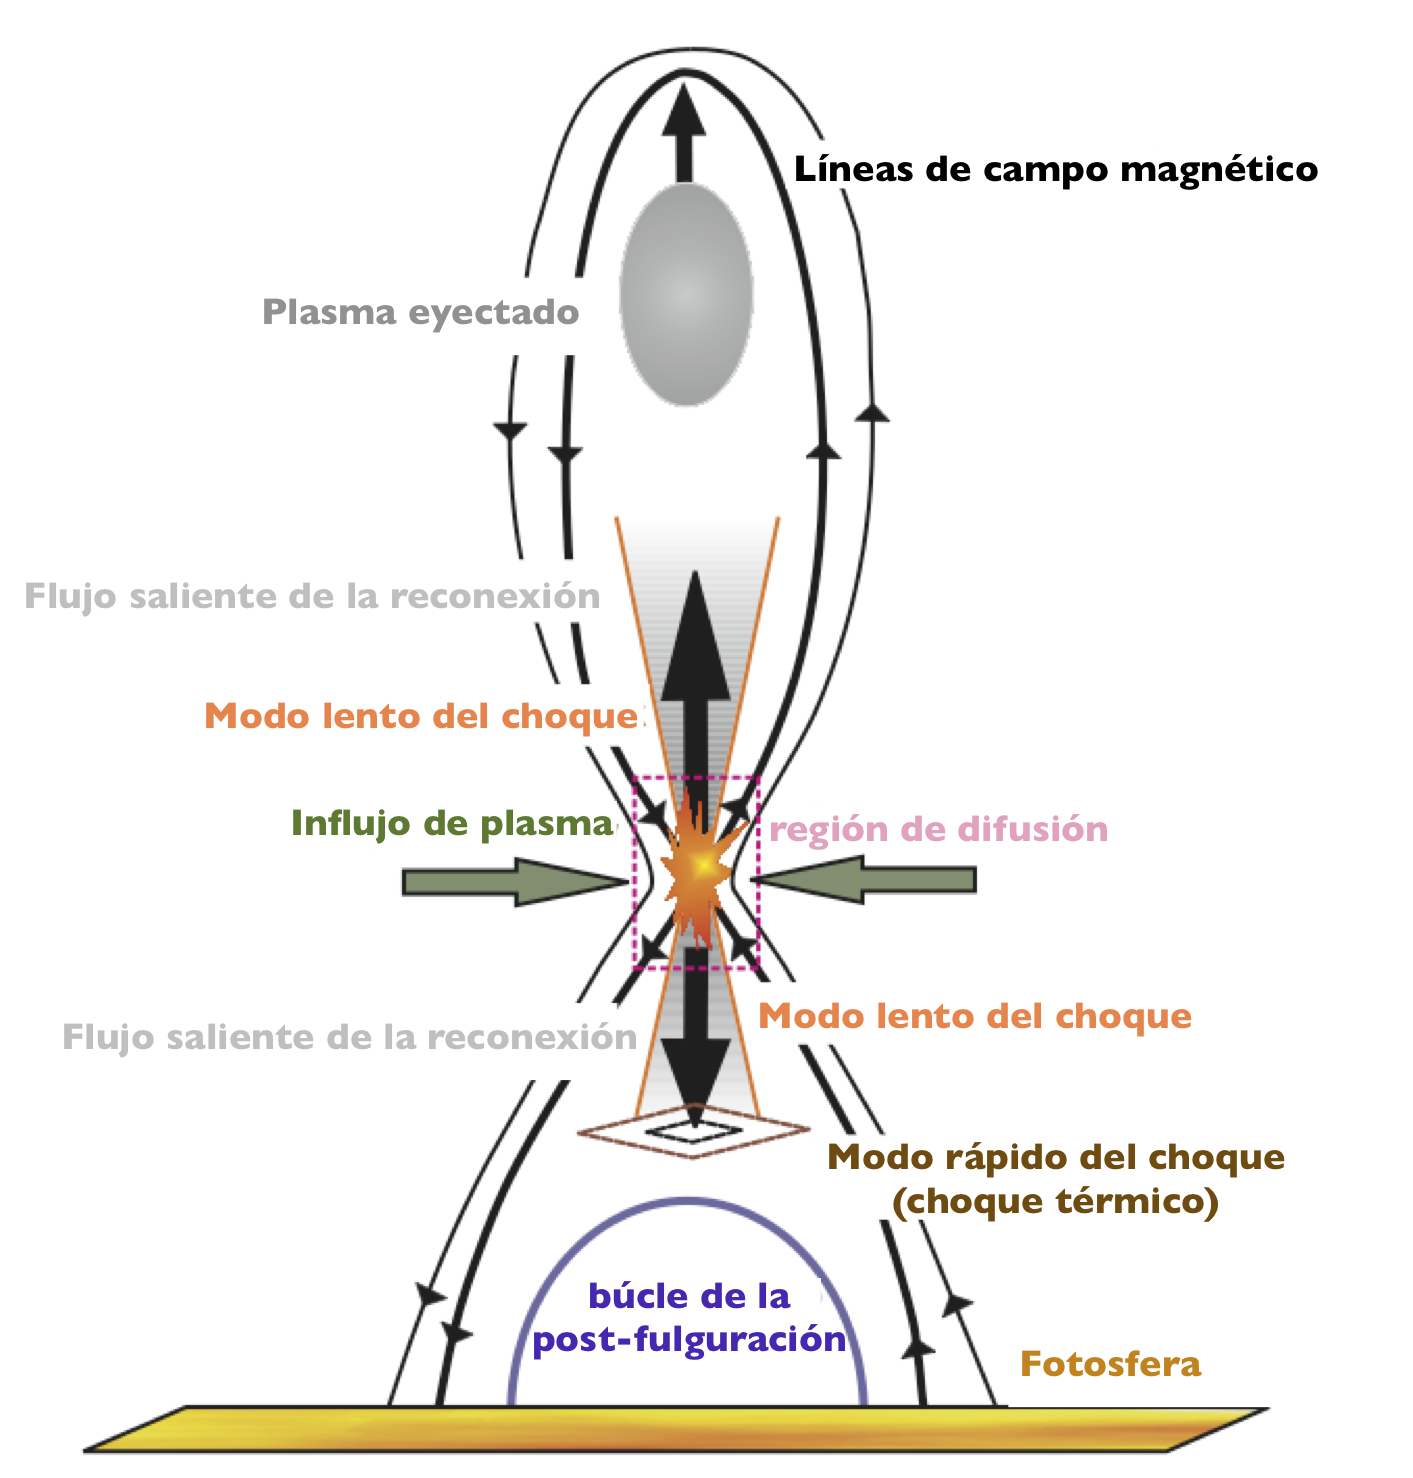
\includegraphics[width=0.65\textwidth]{reconexion.png}
\caption{Se representa esquem\'aticamente el proceso de reconexi\'on magn\'etica asociado a una fulguraci\'on solar. El evento ocurre en la regi\'on de difusi\'on de manera que el plasma local es catapultado hacia arriba y hacia abajo del v\'ertice de reconexi\'on en forma de jets de plasma.}
\label{reconexion}
\end{figure}

Una fulguraci\'on tiene su origen en un proceso de reconexi\'on magn\'etica. Cuando de la capa base de la fotosfera emergen l\'ineas de campo magn\'etico hacia la corona solar se posibilita la formaci\'on de una prominencia que, si tiene una configuraci\'on como la que se muestra en la figura \ref{reconexion}, genera las condiciones necesarias para que se presente un evento de reconexi\'on magn\'etica y, asociado a \'el, una fulguraci\'on solar. As\'i, en ese momento se establece una l\'amina de corriente que, si  excede un valor cr\'itico, provoca que la resistividad se incremente, debido a la excitaci\'on ondulatoria del plasma, originando de esta manera varios lugares de inestabilidad. En este caso la reconexi\'on magn\'etica puede ocurrir en la regi\'on donde la resistividad ha aumentado, i.e. la regi\'on de difusi\'on.

\subsection*{Clasificaci\'on de las fulguraciones}
\addcontentsline{toc}{subsection}{Clasificaci\'on de las fulguraciones}

Las fulguraciones se clasifican seg\'un la intensidad que se registra en rayos-X en un rango espectral que va de 1$\AA\,$a 8$\AA\,$ a trav\'es de los instrumentos de {\it GOES}\footnote{{\it GOES} es el acr\'onimo en ingl\'es de ``{\it Geostacionary Operational Environmental Satellite}'', ver http://www.swpc.noaa.gov/} \citep[]{fletcher2011}. Los valores t\'ipicos de potencia en una fulguraci\'on oscilan entre $10^{-8}$ W/m$^2$ y $10^{-3}$ W/m$^2$ de forma que es apenas natural pensar en una clasificaci\'on en escala logar\'itmica como la que se muestra en la figura \ref{goes}. Adicionalmente cada una de estas clases est\'a dividida en nueve subclases, i.e., la fulguraci\'on de clase X6 que se muestra en la figura \ref{goes}, o sea una intensidad de $6\times10^{-4}$ W/m$^2$, fue tres veces m\'as fuerte que la fulguraci\'on de clase X2 que se muestra en la misma figura, que a su vez fue cuatro veces m\'as fuerte que la fulguraci\'on de clase M5. Un resumen de esta clasificaci\'on se muestra en la tabla \ref{tabla_clas}


\begin{table}[htdp!]
\caption{Clasificaci\'on GOES de las fulguraciones solares}
\begin{center}
\begin{tabular}{|c|c|}\hline
Flujo [Wm$^{-2}$] & Clase GOES \\\hline
$10^{-8}$ & A1 \\
$10^{-7}$ & B1 \\
$10^{-6}$ & C1 \\
$10^{-5}$ & M1 \\
$10^{-4}$ & X1 \\
$10^{-3}$ & X10 \\\hline
\end{tabular}
\end{center}
\label{tabla_clas}
\end{table}

\subsection*{Inyecci\'on de part\'iculas energ\'eticas}
\addcontentsline{toc}{subsection}{Inyecci\'on de part\'iculas energ\'eticas}

Con ayuda de las observaciones llevadas a cabo por los diferentes telescopios espaciales durante las \'ultimas dos d\'ecadas \citep[]{aschwanden2004} se ha podido establecer que en el momento en que ocurre una explosi\'on solar asociada a una fulguraci\'on, una gran cantidad de part\'iculas cargadas el\'ectricamente se aceleran y son llevadas a niveles muy altos de energ\'ia (relativistas) en tan solo unos cuantos segundos, pero el mecanismo por medio del cual se desarrolla este proceso es a\'un tema de debate hoy d\'ia en la rama de la f\'isica solar. Los procesos de colisi\'on, ya sea v\'ia Coulomb o contra part\'iculas el\'ectricamente neutras, son mecanismos en los cuales en vez de existir una ganancia neta de energ\'ia por parte de las part\'iculas incidentes se presenta una p\'erdida. 

\begin{wrapfigure}[22]{r}{0.6\textwidth}
\centering
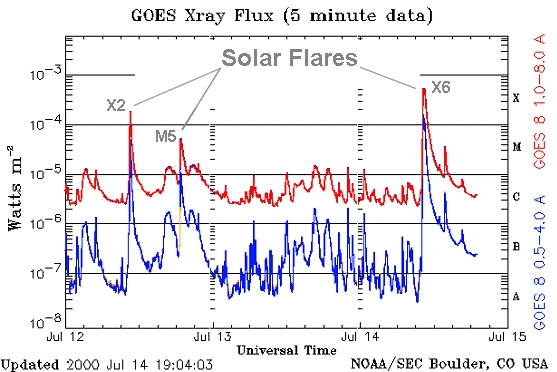
\includegraphics[width=0.58\textwidth]{goes.jpg}
\caption{El diagrama muestra la intensidad en rayos-X dada por {\it GOES} en un periodo de tiempo comprendido entre el 12 de Julio y el 15 de Julio del 2000. Durante este tiempo se observaron unas cuantas fulguraciones de diferentes tipos. Referencia: http://www.spaceweather.com/glossary/images/xray.gif }
\label{goes}
\end{wrapfigure}


Una forma natural de considerar la manera en la que se pueden acelerar estas part\'iculas y abastecerlas de la suficiente energ\'ia es suponiendo que se encuentran sometidas al efecto de un campo el\'ectrico particular. Recientemente muchos trabajos se han encaminado en esta direcci\'on \citep[]{HOLMAN1985,benz1987,ls1993,Tsuneta1998} teniendo alg\'un \'exito solo en el caso de poder reproducir par\'ametros estimados de las observaciones tales como las curvas de luz, los espectros y/o las densidades de part\'iculas. Es importante aclarar que la diferencia m\'as notoria entre estos modelos radica en la forma, lugar y momento en el que consideran la creaci\'on del campo, su topolog\'ia y la magnitud del mismo. Todos estos modelos de aceleraci\'on de part\'iculas est\'an cambiando continuamente a causa del  aumento constante en la calidad de las observaciones, y por ende, las resoluciones espacial y temporal de las mismas. Por ejemplo, hoy en d\'ia RHESSI es el sat\'elite que con una instrumentaci\'on apropiada ha permitido desarrollar investigaciones encaminadas a entender los procesos de aceleraci\'on de part\'iculas, por sus rangos din\'amico y espectral, resoluci\'on espectral y cadencia.\\

Como ya se ha mencionado, cuando se presenta un evento tipo {\it fulguraci\'on solar} un gran n\'umero de iones y electrones son acelerados y llevados a estados energ\'eticos relativistas \citep[]{2004emslie}. Estas part\'iculas se propagan a lo largo de las l\'ineas de campo magn\'etico y si contienen la cantidad de energ\'ia suficiente para alcanzar zonas m\'as densas de la atm\'osfera solar que se encuentran situadas m\'as abajo; estas pueden producir la emisi\'on de rayos X duros y gamma al colisionar con el plasma local \citep[]{Brown1971}. Entonces, durante las fulguraciones la radiaci\'on {\it no-t\'ermica} en rayos-X es producida principalmente v\'ia procesos de frenado {\it Bremsstrahlung} por las part\'iculas energ\'eticas que se propagan a trav\'es de la cromosfera densa. De aqu\'i que el espectro (de fotones) en rayos-X est\'a fuertemente relacionado con el espectro de las part\'iculas aceleradas en este evento. 

\subsection*{Una vista multi-frecuencia de las fulguraciones solares}
\addcontentsline{toc}{subsection}{Una vista multi-frecuencia de las fulguraciones solares}

El Sol luce completamente diferente dependiendo de la longitud de onda en la que se le observe. En la figura \ref{multi-frecuencia} se pueden ver las diferentes caras del Sol (para un mismo tiempo) cuando se observa en el visible (arriba a la izquierda), en H$\alpha$ (arriba a la derecha), en ultravioleta (abajo a la izquierda) y en rayos X (abajo a la derecha). 

La emisi\'on en rayos-X usualmente se origina en la corona, en las fulguraciones solares, o en regiones de la cromosfera alta cuando esta es calentada. En zonas de sol calmo la emisi\'on observada es una emisi\'on t\'ermica continua del plasma caliente y que se da gracias a las transiciones tipo {\it libre-libre} de los iones y electrones que se encuentran all\'i.  La figura \ref{corona-heating} ilustra la temperatura y densidad electr\'onica t\'ipica de la atm\'osfera en regiones de sol calmo \citep[]{benz2002}.\\

La emisi\'on en rayos-X obtenida del Sol se clasifica en rayos-X blandos y rayos-X duros.\\

{\it Rayos-X blandos}: ({\it SXR} por sus siglas en ingl\'es, {\it Soft X Rays}). Se considera que es emisi\'on t\'ermica producida por los iones y electrones energ\'eticos que conforman la atm\'osfera solar y la cual se caracteriza por la temperatura a la que se encuentre el plasma local. Las energ\'ias t\'ipicas de los fotones asociadas a este proceso oscilan en un rango de $\approx 0.1-15$ keV, es decir, en el rango de 0.8 a 124 $\AA$.\\


\begin{SCfigure}
\centering
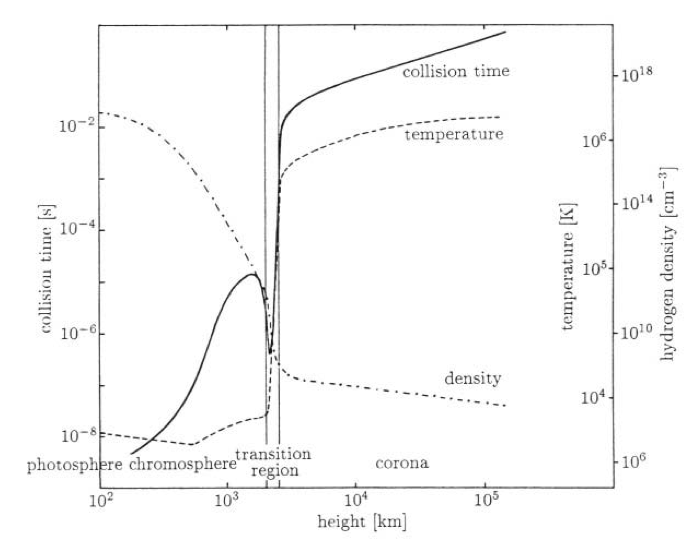
\includegraphics[width=0.48\textwidth]{corona-heating.png}
\caption{Curvas tomadas de \citep[]{benz2002} p\'agina 19. Aunque esta gr\'afica tiene bastante informaci\'on lo que nos interesa son las dos curvas punteadas correspondientes a la variaci\'on de la temperatura y de la densidad de hidr\'ogeno con respecto a la altura en la atm\'osfera solar. Estas curvas muestran una variaci\'on s\'ubita en la as\'i llamada {\it regi\'on de transici\'on} y su comportamiento es determinado suponiendo una regi\'on de sol calmo. La densidad decrece en ocho ordenes de magnitud y la temperatura crece en dos. Estos cambios abruptos a\'un hoy son temas que se consideran problemas abiertos de la f\'isica solar.}
\label{corona-heating}
\end{SCfigure}

{\it Rayos-X duros}: ({\it HXR} por sus siglas en ingl\'es: {\it Hard X Rays}) Es aquella emisi\'on de fotones con energ\'ias por encima de la energ\'ia que caracteriza los SXR, 300 keV (0.04 $\AA$), producidos por radiaci\'on de frenado ({\it Bremsstrahlung}) cuando el jet de part\'iculas aceleradas durante el evento de la fulguraci\'on colisiona con el plasma de la atm\'osfera local, aquello que se conoce en la literatura especializada como {\it thick} y {\it thin target}. Un an\'alisis detallado de las implicaciones f\'isicas asociadas a la emisi\'on en esta banda se encuentra en \citep[]{holman2011}.


\begin{figure}[ht!]
\centering
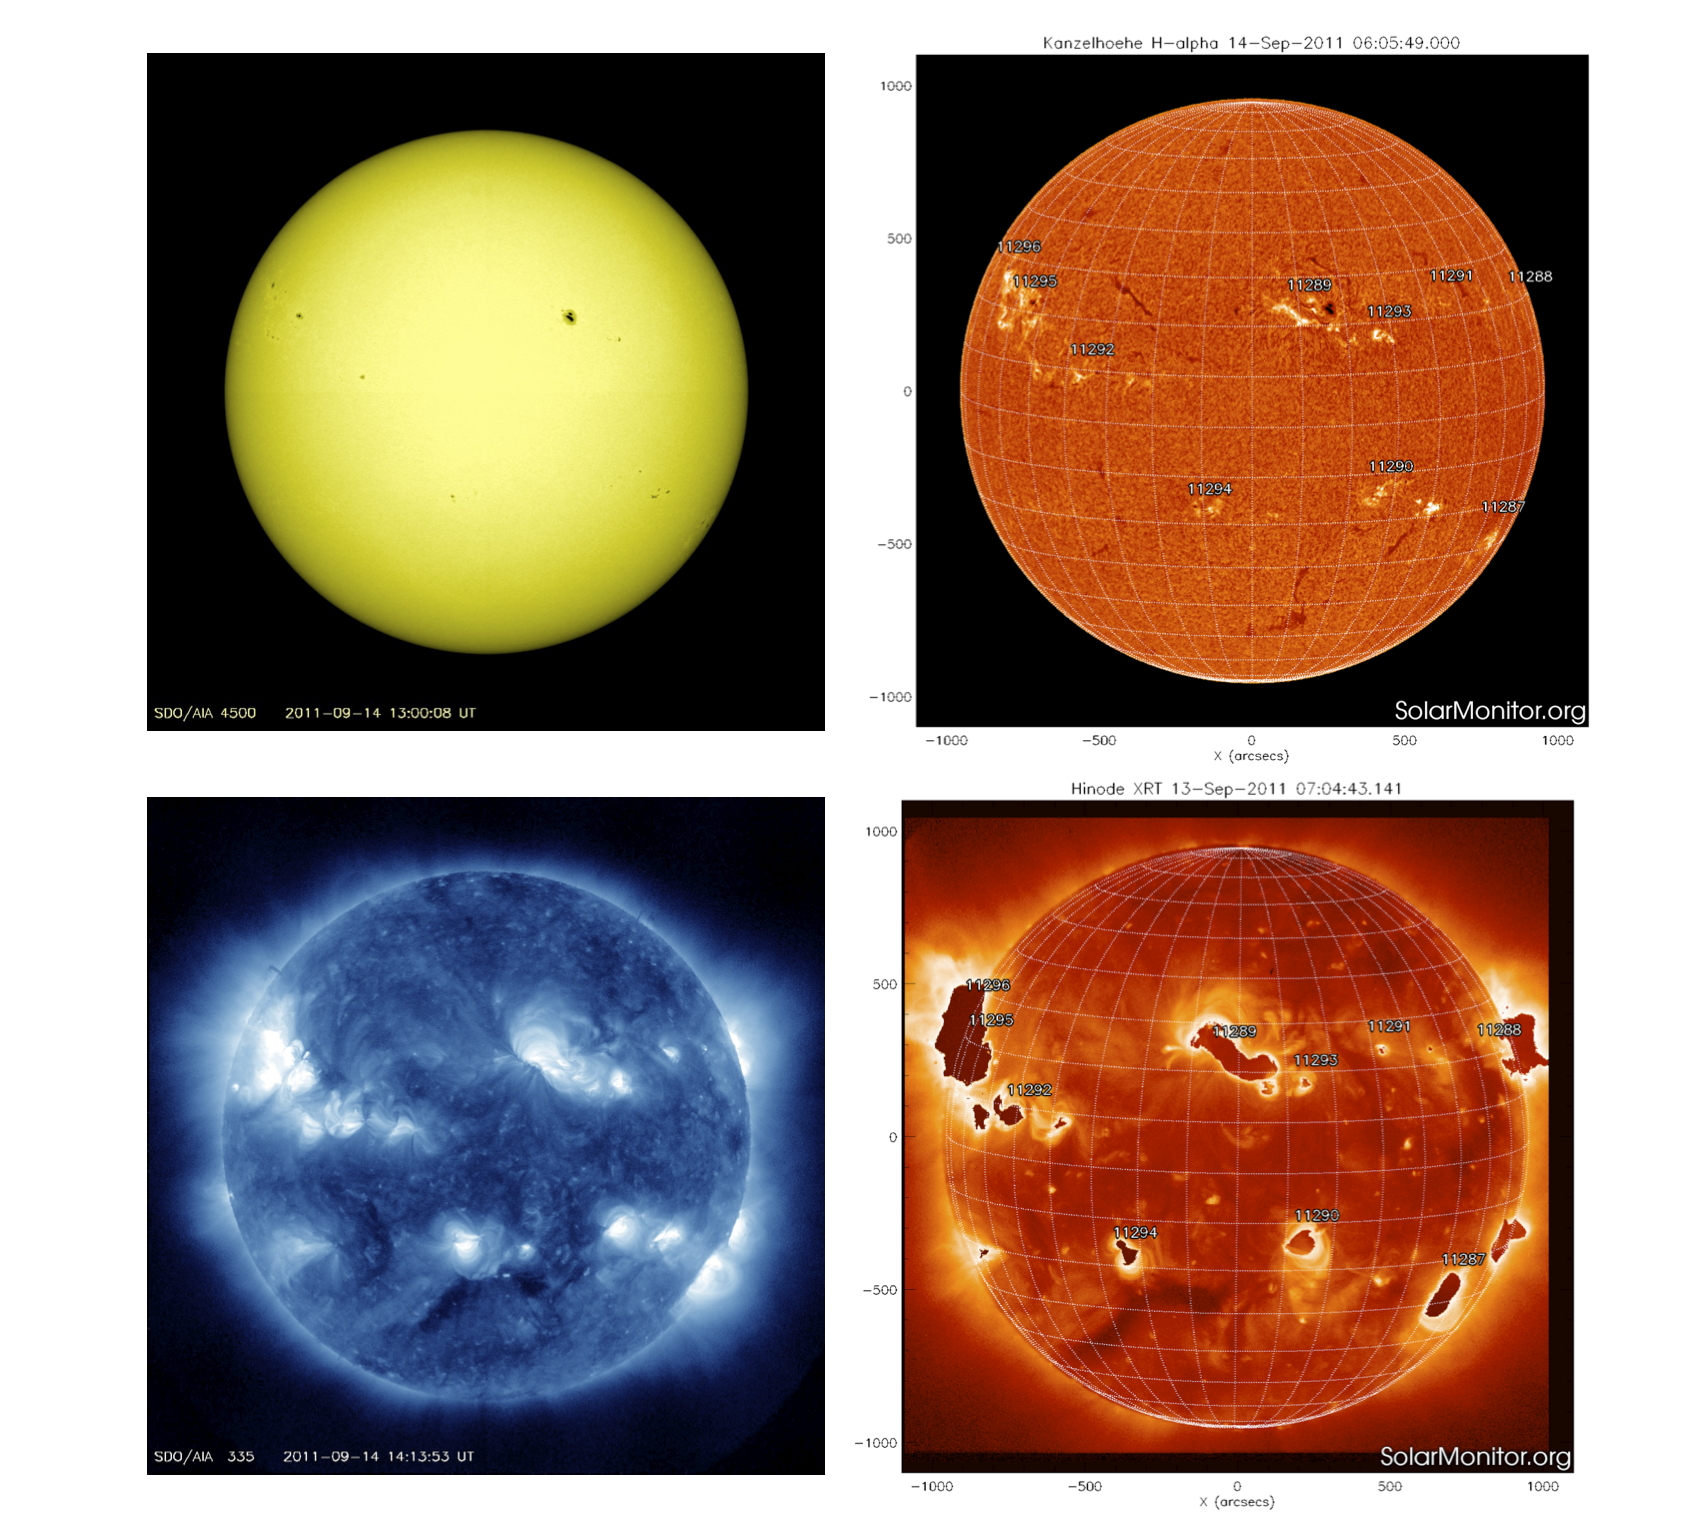
\includegraphics[width=0.91\textwidth]{multifrecuencia.png}
\caption{Visualizaci\'on del disco solar en diferentes bandas del espectro electromagn\'etico para el 14 de Septiembre de 2011. {\it Arriba a la izquierda:} Imagen del Sol en el continuo de luz blanca, mostrando 10 regiones activas, tomada por SDO/HMI (NASA) centrada en $4500\,\AA$. {\it Arriba a la derecha:} Imagen del Sol centrada en la l\'inea de H$\alpha$ ($6562,8\,\AA$) mostrando la estructura de la cromosfera tomada por el observatorio {\it Kanzelhoehe} de Austria. En esta imagen las prominencias se ven como filamentos oscuros sobre el disco solar. {\it Abajo a la izquierda:} Imagen en extremo ultravioleta tomada con un filtro centrado a $335\,\AA$ por SDO/AIA en donde se ilustra la regi\'on alta de transici\'on a una temperatura cercana a los 430.000 K. {\it Abajo a la derecha:} Imagen en rayos-X (centrado a $6\,\AA$) en donde se muestra la corona solar a una temperatura de unos 2 Millones de Kelvin tomada con el {\it Hinode} (Solar-B, JAXA/NASA/PPARC).}
\label{multi-frecuencia}
\end{figure}






\pagestyle{fancy}
\chapter*{Heliosismolog\'ia}
\addcontentsline{toc}{chapter}{Heliosismolog\'ia}


Una pregunta importante en el estudio del Sol es ?`C\'omo pueden hacer los f\'isicos solares conocer el interior solar si el mismo no es visible? La forma de hacerlo es justamente la tarea de la Helio-sismolog\'ia que mediante observaciones y medidas de las oscilaciones vistas en la superficie hace inferencias y prospecciones acerca de las propiedades del interior solar. Las medidas que se pueden obtener son medidas en el cambio de la velocidad superficial v\'ia {\it efecto Doppler} a causa del plasma que se mueve hacia adentro y hacia fuera en la l\'inea de la visual del observador, seg\'un el momento en el que se le observe y el {\it modo de oscilaci\'on} predominante bajo el cual est\'e sometido.\\


\section*{Heliosismolog\'ia local}
\addcontentsline{toc}{section}{Heliosismolog\'ia local}

\begin{wrapfigure}[25]{l}{0.5\textwidth}
\begin{center}
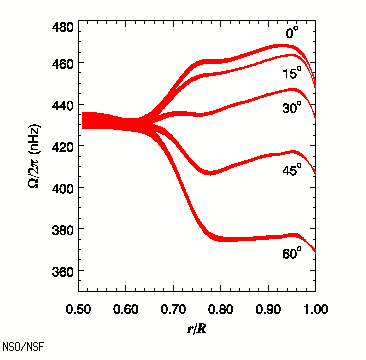
\includegraphics[width=0.5\textwidth]{Tachocline.png}
\caption{Rotaci\'on de la estructura interna solar inferida de los datos heliosismol\'ogicos \citep[]{Thompson1996}.}
\label{fig:rotdiff}
\end{center}
\end{wrapfigure}


% la heliosismologia es una herramienta para estudiar un fen�meno f�sico

%Aparentemente los resultados de Bart sugieren que hay una correlaci�n entre el periodo de las especulas y el periodo fundamental.

% La heliosismologia local fue hecha para tratar de entender la estructura interna de fen�menos locales... por ejemplo una mancha como es una estructura de una mancha por dentro. Como son las cosas por debajo.


%Diagramas de anillo lo �nico que se puede inferiri es la velocidad del sonido... usando un modelo atmosf�rico es que se pueden sacar todos los otros par�metros que se mencionan all�... es un m�todo que se aplica sobre quite sun.


%Cambiar las palabras 3D por tres dimensiones

% Time distance no se limita a los 3mHz

% Duvall gr�fica las croscorrelaciones de las potencias... no es exactamente el diagrama de tiempo.

% revisar articulo de Gizon para lo del time-distance.

%diferenciar: M�todo heliosismol�gico de tiempo distancia. y diagrama tiempo-distancia.

% reescribir la primera parte del subcapitulo 

Dependiendo del tipo de oscilaci\'on en el que se est\'e interesado la {\it heliosismolog\'ia} se divide en {\it global} y {\it local}. Cuando se analizan los modos globales de oscilaci\'on (aquellos que abarcan toda la superficie solar) es posible construir un esquema de la estructura global interna de la estrella. Gracias a esta rama de la f\'isica solar se ha podido lograr establecer, por ejemplo, que la zona de discontinuidad entre la zona radiativa y la zona convectiva conocida como la {\it tacoclina}, aparte de ser una regi\'on en el interior solar donde cambia el mecanismo de transporte de energ\'ia, es tambi\'en un lugar desde el cual el Sol deja de rotar como un cuerpo r\'igido y empieza a hacerlo de forma diferencial y en funci\'on de la latitud heliogr\'afica (ver figura \ref{fig:rotdiff}). Uno de los hallazgos m\'as importantes de esta rama es el llamado {\it modo normal de oscilaci\'on} el cual tiene un periodo cercano a los cinco minutos, una frecuencia asociada de unos $\sim 3$ mHz que ser\'a un valor importante para nosotros en el momento en que toquemos el tema de los mapas de egresi\'on ac\'ustica, y del cual se ha hallado una fuerte correlaci\'on con el periodo de oscilaci\'on de las esp\'iculas \citep[]{DePontieu2004}. Los avances de mayor impacto en esta \'area son expuestos en un art\'iculo de hace una d\'ecada \citep[]{Dalsgaard2002}.\\

La {\it heliosismolog\'ia local} por su lado se centra en el estudio detallado de eventos s\'ismicos mucho m\'as localizados, especialmente sobre aquellos que tienen lugar en regiones activas de la superficie solar. Esto \'ultimo ofrece un nuevo problema a la heliosismolog\'ia y se trata de la forma en la que se desarrolla el tratamiento para dar cuenta de la propagaci\'on de la perturbaci\'on ac\'ustica por debajo de la superficie solar ya que para la determinaci\'on de las propiedades de esa zona hasta entonces se ha apelado exclusivamente a solucionar las ecuaciones hidrodin\'amicas en ausencia de campo magn\'etico, lo cual, por supuesto, deja de ser v\'alido en las regiones activas del Sol que es donde se enfoca el estudio de esta rama. Por otro lado, una ventaja que puede ofrecer el estudio s\'ismico de manchas solares es la posibilidad de desentra\~nar la estructura de estas en el interior solar y a su vez dar visos de la fenomenolog\'ia escondida detr\'as de su aparici\'on y evoluci\'on. Dentro de las prioridades en este momento es encontrar el mejor modelo que de cuenta de la propagaci\'on de una onda ac\'ustica dentro de un plasma acoplado con un campo magn\'etico relativamente fuerte, para enseguida buscar la mejor manera de implementarlo al problema particular de la aparici\'on de un sismo asociado una mancha solar.\\

La Heliosismolog\'ia local es una rama de la f\'isica solar relativamente nueva, desarrollada b\'asicamente durante las \'ultimas dos d\'ecadas desde el reporte por \cite{kz1998}  del primer sismo asociado a una fulguraci\'on tipo X2.6 en la regi\'on activa NOAA 7978. Los datos observacionales para este tipo de an\'alisis han sido tomados por dos instrumentos espaciales y una red de telescopios solares en tierra. Estos son el MDI ({\it Michelson Doppler Imager}) a bordo del SOHO ({\it SOlar and Heliospheric Observatory}) \citep[]{scherrer1995}, el r ecientemente enviado a \'orbita HMI ({\it Helioseismic and Magnetic Imager}) a bordo del SDO ({\it Solar Dynamic Observatory}) \citep[]{kosovichev2007}, y la red de observatorios GONG++ ({\it Global Oscillation Network Group}) \citep[]{harvey1996}. Las im\'agenes que se obtienen son im\'agenes del disco solar completo y la resoluci\'on varia de un instrumento al otro siendo las im\'agenes de MDI y de GONG archivos de $1024\times1024$ p\'ixeles y las de HMI de $4096\times4096$ p\'ixeles, teniendo en cuenta que para los observatorios en tierra se debe considerar adem\'as el efecto producido por la turbulencia atmosf\'erica sobre los datos de ciencia.\\

Para el an\'alisis heliosimol\'ogico local de los Dopplergramas\footnote{Se llaman Dopplergramas a los fotogramas del Sol 2D en los que se marcan diferencias en la velocidad en la componente de la visual.} obtenidos con los instrumentos anteriormente mencionados se han desarrollado una serie de m\'etodos diferentes entre los que se obtiene un acercamiento prospectivo y/o din\'amico. Entre los m\'as utilizados hoy en d\'ia se encuentran el {\it an\'alisis por diagrama de anillos}, los {\it diagramas tiempo-distancia (time distance)} o diagramas TS como se encuentra en alguna literatura, la {\it holograf\'ia ac\'ustica}, la t\'ecnica de {\it Fourier-Hankel}, cada una de ellas utilizada para un fin espec\'ifico que a continuaci\'on discutimos brevemente.


\subsection*{Diagrama de anillos}
\addcontentsline{toc}{subsection}{Diagrama de anillos}

Esta t\'ecnica se basa en cubrir varias regiones peque\~nas en forma de anillos sobre la superficie solar. En cada una de las zonas peque\~nas se infieren dos cantidades f\'isicas que por lo general son la velocidad del sonido y la densidad de masa como funci\'on de la profundidad, y basados en estas, se determinan las otras cantidades como presi\'on y temperatura. Haciendo una combinaci\'on de la informaci\'on de cada zona peque\~na es posible construir una visualizaci\'on en 3D de la estructura interna. Este m\'etodo ha sido usado t\'ipicamente para encontrar el l\'imite externo de la zona convectiva a unos $\sim 30$ Mm de profundidad (siendo esta profundidad usualmente medida desde la alta fotosfera) \citep[]{haber2002}.\\

La forma de proceder es construyendo un espectro de potencia en 3D para cada una de las regiones peque\~nas lo cual resulta en una imagen de anillo \citep[]{hill1988}.\\

Las propiedades del plasma bajo la superficie solar son inferidas mediante el an\'alisis en las variaciones en frecuencias de los espectros de potencia. La presencia de un flujo interno introduce un corrimiento Doppler en las frecuencias, y por lo tanto un cambio en la forma de los anillos. La forma en la que se afectan los diferentes {\it modos} da un indicativo de la profundidad y dimensiones del flujo interno \citep[]{gonzalez2006}. N\'otese que los anillos mostrados en la figura \ref{fig:rotdiff} son construidos a frecuencias muy cercanas a la que hoy d\'ia sabemos que corresponde al modo normal (de resonancia) en el Sol que es el del orden de los cinco minutos \citep[]{goldreich1977} (recordemos que $\nu_{fund}=\frac{1}{T_{fund}}=\frac{1}{300\,s}$=3,3\,\text{mHz}).

\begin{figure}[ht!]
\begin{center}
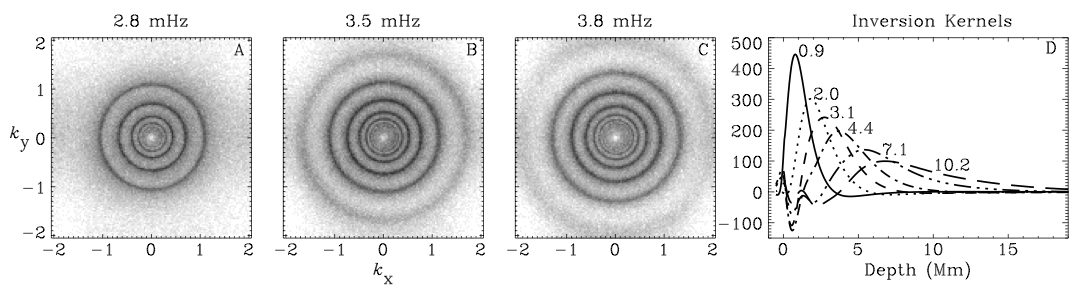
\includegraphics[width=1.0\textwidth]{ringdiagram.png}
\caption{(a) - (c) Corte transversal de un espectro de potencias de un diagrama de anillo tridimensional para tres frecuencias diferentes. Cada anillo corresponde a un \'unico orden radial $n$. (d) N\'ucleos representativos para una inversi\'on basada en los diagramas de anillo graficados como funci\'on de la profundidad bajo la fotosfera \citep[]{haber2002}.}
\label{fig:rotdiff}
\end{center}
\end{figure}

\subsection*{Diagrama de Tiempo-Distancia}
\addcontentsline{toc}{subsection}{Diagrama de Tiempo-Distancia}


Esta t\'ecnica expuesta por primera vez por \cite{duvall1993} se basa en la medida de la trayectoria descrita por una onda ac\'ustica (vista v\'ia efecto Doppler) que viaja de un punto a otro sobre la superficie solar. Esta t\'ecnica es muy usada hoy en d\'ia para la determinar si un cierto evento de fulguraci\'on solar tiene, o no, asociado un sismo. La forma de implementarlo es tomar la imagen Doppler del disco solar obtenida con alguno de los instrumentos dispuestos para esto y recortar la imagen en la zona en donde se produjo la fulguraci\'on para luego centrar sobre ella un c\'irculo cuyo radio va hasta unos 20 Mm y hacer las restas entre im\'agenes consecutivas para encontrar de esta manera la se\~nal de una fuerte variaci\'on ac\'ustica que se propaga desde el centro del c\'irculo hacia afuera de \'el.\\

Este protocolo ya se ha sistematizado y por ejemplo el equipo de la Universidad de Stanford en California encargado del almacenamiento y distribuci\'on de los datos tomados por {\it HMI/SDO} ha construido una serie de programas que cada ocho horas hace un barrido del disco en las fulguraciones que tuvieron lugar durante ese lapso de tiempo y aplican este m\'etodo sobre los Dopplergramas denotados como {\it near-real-time} para determinar la existencia o no de sismos solares \citep[]{zhao2011}. Esto resulta ser una ventaja apreciable ya que se puede informar a la comunidad cient\'ifica mundial la aparici\'on de un nuevo sismo solar en tan solo unas pocas horas despu\'es de que ocurra, tal como ocurri\'o con el primer sismo del ciclo 24 asociado a la fulguraci\'on tipo X2.2 de la regi\'on activa NOAA 1158 que tuvo lugar el 15 de Febrero de 2011 y que tan solo cuatro horas despu\'es fue reportado por Kosovichev \citep[]{kosovichev2011}.\\

\begin{figure}[!ht]
\begin{center}
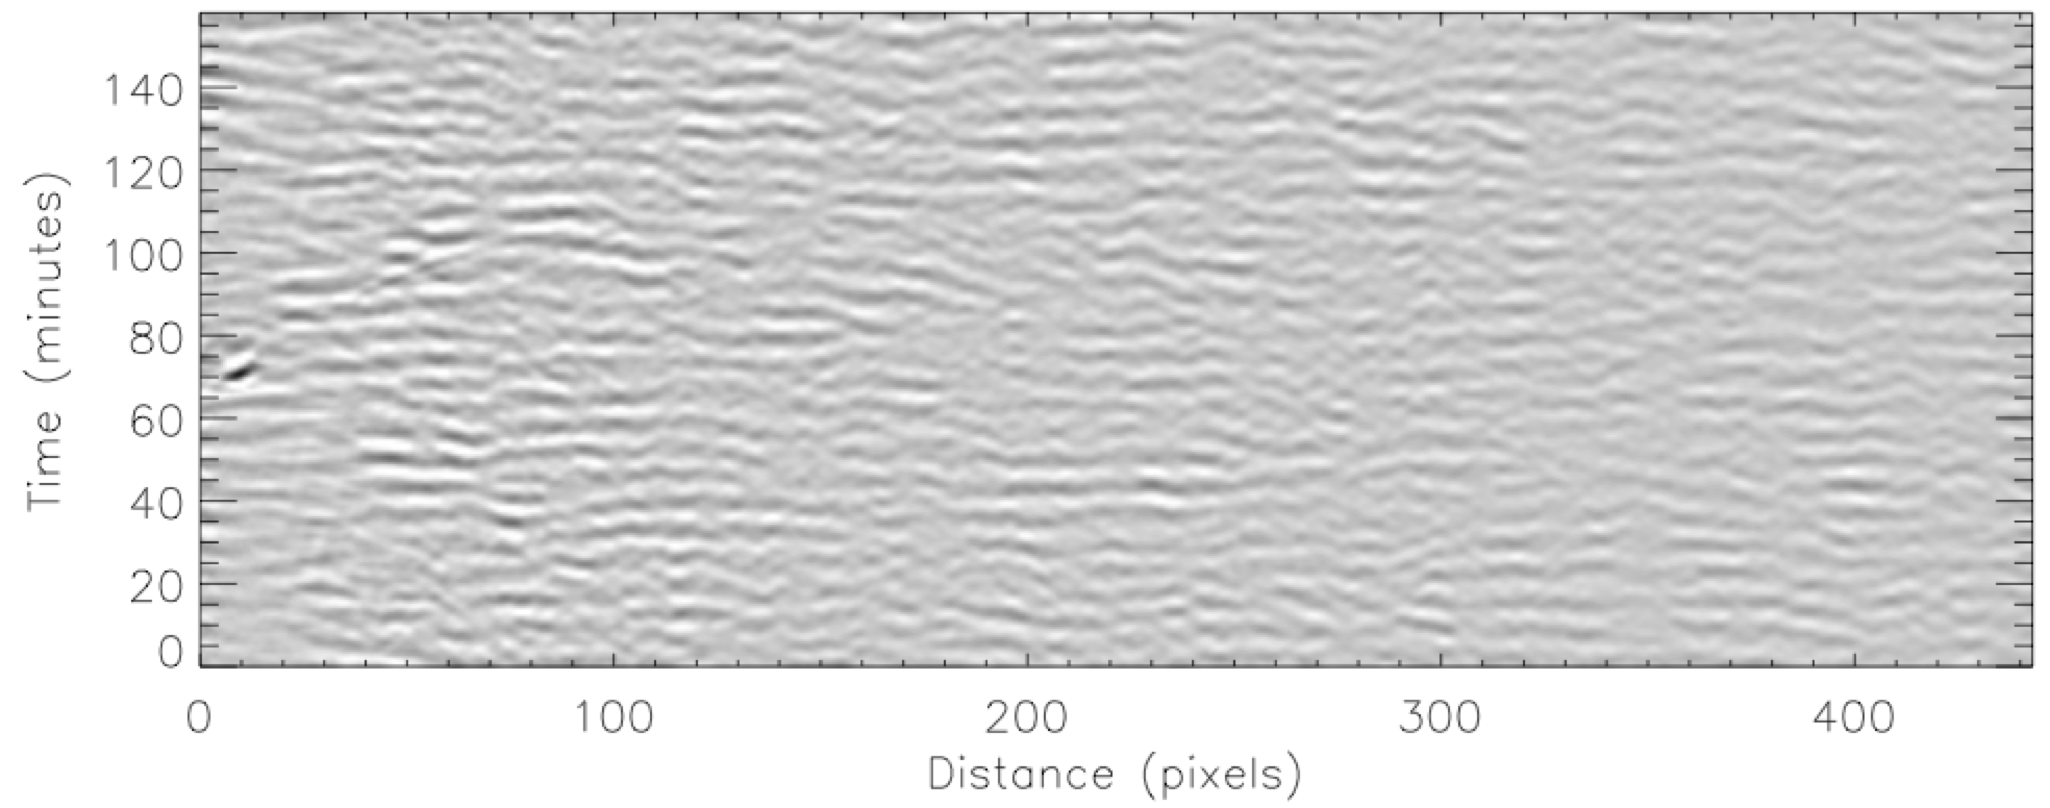
\includegraphics[width=1.0\textwidth]{td_plot_2011_02_15.png}
\caption{Diagrama TD para la fulguraci\'on solar clase GOES X2.2 del 15 de Febrero de 2011. Podemos discernir una se\~nal ac\'ustica ubicada al lado izquierdo que incrementa su velocidad al transcurrir el tiempo.}
\label{fig:td}
\end{center}
\end{figure}

Los principales progresos en la heliosismolog\'ia de la d\'ecada pasada ocurrieron a trav\'es del an\'alisis de los modos normales de oscilaci\'on \citep[]{dalsgaard1991}, esto debido principalmente a la dificultad de observar el viaje temporal de se\~nales ac\'usticas que se confunden con el ruido provocado por los muchos modos de oscilaci\'on que llegan a la superficie solar. Esto entra en contraste con la forma de hacer s\'ismica en nuestro planeta en donde mediante la medida de diferencias de tiempo y diferencias de distancia medidas a trav\'es de diferentes estaciones ubicadas en varios puntos de la superficie terrestre se puede desarrollar una prospecci\'on del subsuelo mediante el an\'alisis espacio temporal de estas se\~nales \citep[]{gubbins1990}.  La t\'ecnica del diagrama Tiempo-Distancia trata de emular esta forma de hacer s\'ismica aqu\'i en la tierra y haciendo uso de los datos de mejor resoluci\'on y observando eventos de fulguraciones solares puede seguir la respuesta sobre la superficie de este tipo de se\~nales como lo reportaron por primera vez \cite{kz1998}.\\

La causa de la perturbaci\'on s\'ismica que da lugar a las ondas vistas despu\'es de un evento de fulguraci\'on solar es un problema abierto de la f\'isica solar que es discutido en los m\'as importantes congresos que se celebran en est\'a \'area y a donde asisten los cient\'ificos m\'as reconocidos y de m\'as amplia trayectoria que trabajan en estos temas \citep[]{zharkova2011a}. Para efectos de entender la forma en la que un frente de 	onda ac\'ustica se propaga por el interior solar para luego ser registrada en una diagrama TD vamos a suponer simplemente que la fuente s\'ismica existe, que es muy fuerte y que est\'a bien localizada.\\

La forma en la que ampliamente se concibe la trayectoria de una onda ac\'ustica cuya fuente est\'a ubicada cerca de la superficie solar es esquematizada en el diagrama de rayos de la figura \ref{fig:td}. Una fuente que tiene lugar en el punto $a$ de la superficie solar es el punto de partida de un rayo que es refractado debido al incremento de la velocidad del sonido local del medio en el que se propaga hasta invertir su direcci\'on radial y llegar al punto $c$. Una vez llega a $c$ se encuentra con un cambio brusco en la densidad local, raz\'on por la cual la onda es reflejada y contin\'ua una trayectoria similar hacia otro punto sobre la superficie solar. De esta manera es como se presenta una correlaci\'on entre el frente de onda visto en $c$ y el punto $a$ desde el cual se origin\'o. La distancia que se observa es la que est\'a sobre la superficie $\Delta$ pero claramente el camino recorrido es $b$ a trav\'es del interior solar. Si la fuente ac\'ustica tuvo lugar en el tiempo $t$, entonces decimos que el tiempo caracter\'istico que tarda el frente de onda de ir desde el punto $a$ hasta el punto $c$ es $T$ y al que se le conoce como el {\it tiempo de viaje}. A pesar de esta relaci\'on directa entre los dos puntos sobre la superficie solar $a$ y $c$, las se\~nales que se observan se ven afectadas por un ruido apreciable introducido por todas aquellas perturbaciones {\it extras} que presentan de forma aleatoria a lo largo del camino $b$ y que a pesar de ser de menor intensidad, tambi\'en tienen una respuesta que es vista en los mismos dos puntos $a$ y $c$. La literatura se refiere a esta interferencia como el {\it problema de oblicuidad}. Es por esta misma raz\'on que no se puede construir un espectro de potencia unidimensional en una l\'inea de p\'ixeles definida sobre una imagen solar, sino que en vez de esto se debe realizar un an\'alisis que abarque una circunferencia centrada en la fuente del sismo.\\

\begin{wrapfigure}[22]{l}{0.45\textwidth}
\begin{center}
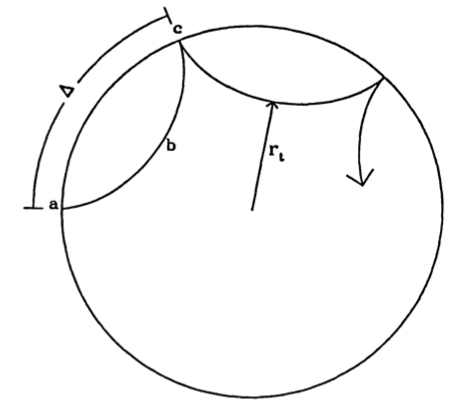
\includegraphics[width=0.42\textwidth]{td.png}
\caption{Esquema que muestra el camino por el que se propaga una onda sonora a lo largo del interior solar. Tomado de \citep[]{duvall1995}}
\label{fig:td}
\end{center}
\end{wrapfigure}

Los primeros trabajos en los que se implement\'o este m\'etodo TD se encontraron {\it tiempos de viaje} del orden de los 75 minutos y distancias $\Delta$ del orden de 25 grados de arco heliosf\'ericos \citep[]{duvall1995} mucho mayor a los tiempos y distancias reportados en los sismos asociados a eventos de fulguraci\'on solar en las vecindades de las manchas solares (ver por ejemplo \citep[]{kosovichev2011,martinez-oliveros2009,mo2008d,metal2006b,detal2006}) en los que los tiempos de viaje son del orden de los 30 minutos y las distancias son cercanas a los 5 o 10 grados heliosf\'ericos. La raz\'on es que a pesar de que el diagrama TD es un m\'etodo centrado en una localidad finita de la superficie solar, en un principio fue usado dentro del marco de la heliosismolog\'ia global bajo la suposici\'on de un n\'umero de {\it Reynolds magn\'etico} grande de manera que son los {\it modos-p} la base sobre la cual el frente de onda ac\'ustico se propaga. Claramente, el plasma confinado en una mancha solar se comporta siguiendo un r\'egimen magn\'etico de manera que las l\'ineas de campo magn\'etico se encuentran congeladas y los modos-p de vibraci\'on son amortiguados fuertemente \citep[]{braun1988,dsilva1995}.\\

Los diagramas de tiempo-distancia trabajados por \cite{duvall1995} est\'an centrados principalmente en un sector de {\it Sol calmo} pero la perturbaci\'on ac\'ustica que se propaga con el tiempo logra entrar luego en una regi\'on activa en donde se visualiza una fractura de la trayectoria y despu\'es de un corto tiempo se observa una disminuci\'on en la intensidad de la se\~nal y una descomposici\'on en su banda de l\'ineas que, se cree, es debido a la presencia de campo magn\'etico dentro de la mancha a trav\'es de la cual contin\'ua propag\'andose la perturbaci\'on. Esto sugiere que la forma en la que se da esta fractura y la posterior aparici\'on de una banda de curvas puede estar relacionada fuertemente con la estructura interna de la mancha solar y es esta la principal raz\'on por la que hoy d\'ia es un tema que genera un gran apetito cient\'ifico para los f\'isicos solares, pues un estudio detallado de este fen\'omeno podr\'ia ayudar a construir un mayor entendimiento de la estructura sub-superficial del Sol.\\

Para explicar la disminuci\'on de la intensidad de la se\~nal ac\'ustica, una vez la perturbaci\'on entra a la mancha solar, se apela a pensar en fen\'omenos de difusi\'on ac\'ustica que aten\'uen la onda. Para dar cuenta de esto desde un acercamiento netamente fenomenol\'ogico se hacen algunas hip\'otesis como que a trav\'es de la mancha solar, y de forma completamente perpendicular, atraviesa un tubo magn\'etico monol\'itico que incrementa la disipaci\'on de los modos ac\'usticos al pasar por las capas resonantes y el un conglomerado de fibrillas internas del tubo adem\'as de la atenuaci\'on debida a la conversi\'on de modos {\it ac\'usticos} a modos {\it magneto-ac\'usticos}. Una revisi\'on detallada de la matem\'atica propuesta para describir esta din\'amica se encuentra en \cite{spruid1992,dsilva1995,dsilva1996,dsilva2001} y \cite{kosovichev2011td}.\\

Una de las debilidades m\'as remarcadas de este m\'etodo es aquella que concierne al ruido que se filtra en los diagramas TD como bien se puede ver, por ejemplo, de aquel que construimos para el evento del 15 de Febrero de 2011 (ver figura \ref{fig:td}) y m\'as a\'un la {\bf raz\'on se\~nal-ruido} de la supuesta propagaci\'on ac\'ustica que se registra. En aras de dar soluci\'on a este problema se ha tratado de caracterizar el ruido ac\'ustico considerando a los mecanismos de excitaci\'on de los modos como fen\'omenos de naturaleza estoc\'astica que generan oscilaciones estacionarias y homog\'eneas sobre toda la superficie solar. De esta manera es posible construir una matriz de covarianza entre las medidas del tiempo de viaje y la inversi\'on ac\'ustica que resulta de este tipo de an\'alisis:

\begin{align}
C(\mathbf{x}_1,\mathbf{x}_2,t_j)=\frac{h_t}{T-|t_j|}\sum_i\phi(\mathbf{x}_1,t_i)\phi(\mathbf{x}_2,t_i+t_j),
\end{align}

\noindent donde $\phi(\mathbf{x},t)$ denota la se\~nal ac\'ustica filtrada observada para un punto $\mathbf{x}$ en un instante\footnote{Este filtrado se realiza mediante la aplicaci\'on de un par de operadores en el dominio del espacio de Fourier del conglomerado de datos observados que generalmente es la remoci\'on de todas aquellas oscilaciones que son m\'ultiplos enteros del modo fundamental de oscilaci\'on y un filtro Gaussiano en fase con la velocidad de la forma $\exp[-(\omega/k-v)^2/(2s^2)]$ siendo $v=36.5\,\text{km s}^{-1}$ y $s=2.5\,\text{km s}^{-1}$.} $t$, $h_t$ es la cadencia del instrumento con el que son tomadas las im\'agenes, $t_j=jh_t$ con $j\,\epsilon\, Z$, y $T$ es el tiempo total sobre el cual se est\'a haciendo el an\'alisis. Un trabajo completo en el que se desarrolla este m\'etodo de limpieza del ruido en la se\~nal y se compara con datos observacionales reales obtenidos con MDI/SOHO es mostrado en \cite{gizon2004}. Como vemos el proceso de filtrado de la se\~nal ac\'ustica genera una repercusi\'on apreciable sobre las medidas de manera que se debe tener en cuenta a la hora de intentar hacer alguna interpretaci\'on f\'isica de las observaciones, como bien lo indican \cite{braun2008,chou2009,salabert2009} y \cite{donea2011}. Este es un m\'etodo que se ha convertido en una herramienta potente de la f\'isica solar, pero que a\'un hoy en d\'ia se discuten sus problemas, como fue el caso del \'ultimo encuentro {\it AGU-2010} ({\it American Geophysical Union}) en donde \cite{duvall2010} expuso el estado del arte de este tema.

\section*{Holograf\'ia heliosismol\'ogica}
\addcontentsline{toc}{section}{Holograf\'ia heliosismol\'ogica}

El m\'etodo de {\it holograf\'ia heliosismol\'ogica} es una t\'ecnica cuya finalidad es la reconstrucci\'on tridimensional de la morfolog\'ia interna de la atm\'osfera solar basandose en la propagaci\'on de los modos-p y la forma en que estos se registran en la superficie del Sol. En Octubre de 1997 Chang y sus colaboradores proponen el m\'etodo llamado {\it imaginolog\'ia ac\'ustica} que consiste en la observaci\'on del ruido ac\'ustico sobre la superficie solar suponiendo que ha sido generado de forma homog\'enea en su interior de manera que (asumiendo adem\'as un primer modelo de la estructura interna de la capa m\'as externa del Sol, la {\it atm\'osfera solar}) si no hubiese ning\'un tipo de obst\'aculo las se\~nales alcanzar\'ian la superficie con cierta fase. El no encontrar las se\~nales ac\'usticas con la fase esperada supondr\'ia la existencia de un obst\'aculo ``{\it \'optico}'' interno y la forma de dimensionarlo ser\'ia justamente aplicando un m\'etodo an\'alogo al usado en \'optica cl\'asica cuando con ayuda de un montaje \'optico se registra la se\~nal de una fuente de luz en cuyo camino \'optico se ha atravesado un obst\'aculo que dispersa los rayos. Esta t\'ecnica fue inicialmente pensada para poder generar la imagen de prospecci\'on interna de inhomogeneidades en el plasma solar tales como las que se presentan en el surgimiento de manchas solares \citep[]{chang1997}. Para ese mismo a\~no los doctores Charles Lindsey y Douglas Braun publican un art\'iculo en el que por primera vez proponen la {\bf holograf\'ia heliosismol\'ogica} como un m\'etodo de prospecci\'on ac\'ustica que permite la ubicaci\'on de la fuente de sismos fuertemente localizados en la superficie del Sol \citep[]{lindsey1997}.\\


\begin{wrapfigure}[28]{l}{0.45\textwidth}
\begin{center}
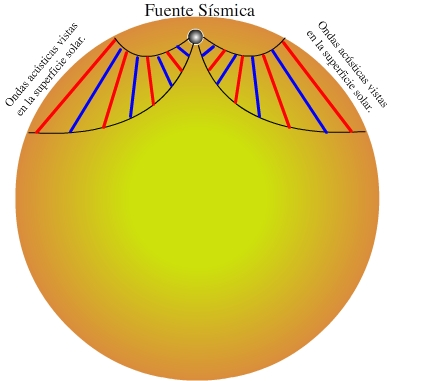
\includegraphics[width=0.42\textwidth]{helioholography.jpg}
\caption{Figura que representa la propagaci\'on de una se\~nal ac\'ustica en el interior solar cerca de la superficie. El dibujo se ha exagerado un poco para hacer \'enfasis en la retro-dispersi\'on que se presenta producto del incremento gradual de la densidad de masa con la profundidad, as\'i como tambi\'en del \'indice {\it \'optico} del medio. Las l\'ineas azules y rojas representan picos y valles de la se\~nal. Se asume un medio cuyas propiedades f\'isicas cambian \'unicamente con la direcci\'on radial.}
\label{fig:holografia}
\end{center}
\end{wrapfigure}


Mucho del tratamiento matem\'atico que se usa en la {\bf holograf\'ia ac\'ustica} es an\'alogo y tomado del formalismo definido sobre la holograf\'ia \'optica propuesta por el cient\'ifico H\'ungaro-Brit\'anico {\it Dennis Gabor} en 1947 y por el cual gan\'o el premio nobel de f\'isica en 1971 \citep[]{collier1971}. En este contexto, el registro de un patr\'on dos-dimensional generado por una superposici\'on de ondas sonoras se considera un {\bf holograma ac\'ustico}. Entonces, haciendo uso de estos {\it hologramas} es posible realizar una prospecci\'on del campo de ondas ac\'usticas que han viajado a trav\'es de un espacio tridimensional del cual se conocen sus caracter\'isticas generales como composici\'on y topolog\'ia\footnote{La {\it topolog\'ia} del medio por el cual se propagan las ondas ac\'usticas cobra una importancia sobresaliente cuando la propagaci\'on se hace sobre un medio que no es isotr\'opico y/o homog\'eneo,  ya que la din\'amica de propagaci\'on de las ondas cambia completamente y empieza a depender por ejemplo de la direcci\'on en la que se propague un frente de onda.}.\\

\noindent El caso m\'as sencillo de suponer es un medio de propagaci\'on uniforme y homog\'eneo dentro del cual se encuentra una fuente de ondas ac\'usticas que se propagan y son registradas en alg\'un lugar durante un periodo de tiempo determinado\footnote{Obviamente la atm\'osfera solar no es un medio uniforme y homog\'eneo a trav\'es del cual se propagan las ondas; por esta raz\'on, para poder hacer holograf\'ia ac\'ustica es ineludible ajustarse a un modelo de atm\'osfera estelar.}. En general, un holograma es generado cuando sobre una superficie ``{\it plana}'' se graba la superposici\'on de la llegada de dos o m\'as ondas provenientes de iluminar el objeto de estudio desde diferentes lugares (diferentes {\it perspectivas}). Para poder obtener un holograma ac\'ustico asociado a un evento de sismo localizado en la superficie solar se hacen un par de suposiciones moderadas para crear un primer acercamiento a esta construcci\'on. Primero se supone una atm\'osfera solar cuyas propiedades f\'isicas no cambian con la latitud y la longitud heliogr\'aficas; esto es, se dice que por ejemplo la densidad cambia solo con la profundidad de la atm\'osfera solar, siguiendo por ejemplo un modelo como el propuesto por \cite{benz2002} (ver figura \ref{corona-heating}). Adem\'as, se plantea una fuente s\'ismica muy bien localizada ({\it casi-puntual}) en el interior solar, de manera que hay una cierta simetr\'ia en las ondas cuando salen de all\'i. Para analizar la forma en la que aplica esta t\'ecnica sobre la superficie solar, consideremos la situaci\'on planteada en la figura \ref{fig:holografia}. All\'i se presenta una fuente de ondas ac\'usticas cerca de la superficie solar. La parte de la se\~nal sonora que va hacia adentro del Sol sufre una retro-dispersi\'on a causa del aumento de la densidad de masa, a lo cual se asocia tambi\'en un aumento gradual en el valor del \'indice ``{\it \'optico}'' del medio de propagaci\'on\footnote{La manera en la que la fuente de la se\~nal ac\'ustica es generada es un tema de fuerte debate a\'un hoy en d\'ia y su discusi\'on se present\'o en el subcap\'itulo de {\bf sismicidad asociada a fulguraciones solares}.}.\\

El formalismo te\'orico detr\'as de la holograf\'ia ac\'ustica es relativamente simple y completamente an\'alogo al usado en holograf\'ia \'optica. Un frente de onda definido sobre una longitud de onda part\'icular se puede representar mediante un n\'umero complejo $\mathbf{U}$, en donde la amplitud y la fase del frente de onda son el valor absoluto y el \'angulo del n\'umero complejo respectivamente. Si sobre la ``{\it pantalla}'' en la que se construye el holograma est\'an incidiendo dos frentes de onda provenientes de dos lugares distintos desde los cuales se ilumina el objeto, cada uno de estos frentes de onda puede ser representado por un n\'umero complejo que llamamos $\mathbf{U}_1$ y $\mathbf{U}_2$, de manera que la combinaci\'on de estos dos se reduce a su suma, $\mathbf{U}_1+\mathbf{U}_2$. La energ\'ia de esta superposici\'on de rayos est\'a dada por

\begin{align}\label{u1+u2}
|\mathbf{U}_1+\mathbf{U}_2|^2=|\mathbf{U}_1|^2+|\mathbf{U_2}|^2+\mathbf{U}_1\mathbf{U}_2^*+\mathbf{U}_1^*\mathbf{U}_2
\end{align}

\noindent en donde los dos primeros t\'erminos de la derecha son las intensidades de las ondas $\mathbf{U}_1$ y $\mathbf{U}_2$, mientras que los dos \'ultimos t\'erminos representan las intensidades adicionales debido a la interferencia entre los dos frentes de onda. Cuando el rayo del objeto y el rayo de referencia provienen de direcciones apreciablemente diferentes, los frentes de onda de la imagen virtual, real y de referencia emergen con diferentes \'angulos siendo posible reconstruir el objeto y verlo claramente.\\

\begin{wrapfigure}[16]{r}{0.53\textwidth}
\begin{center}
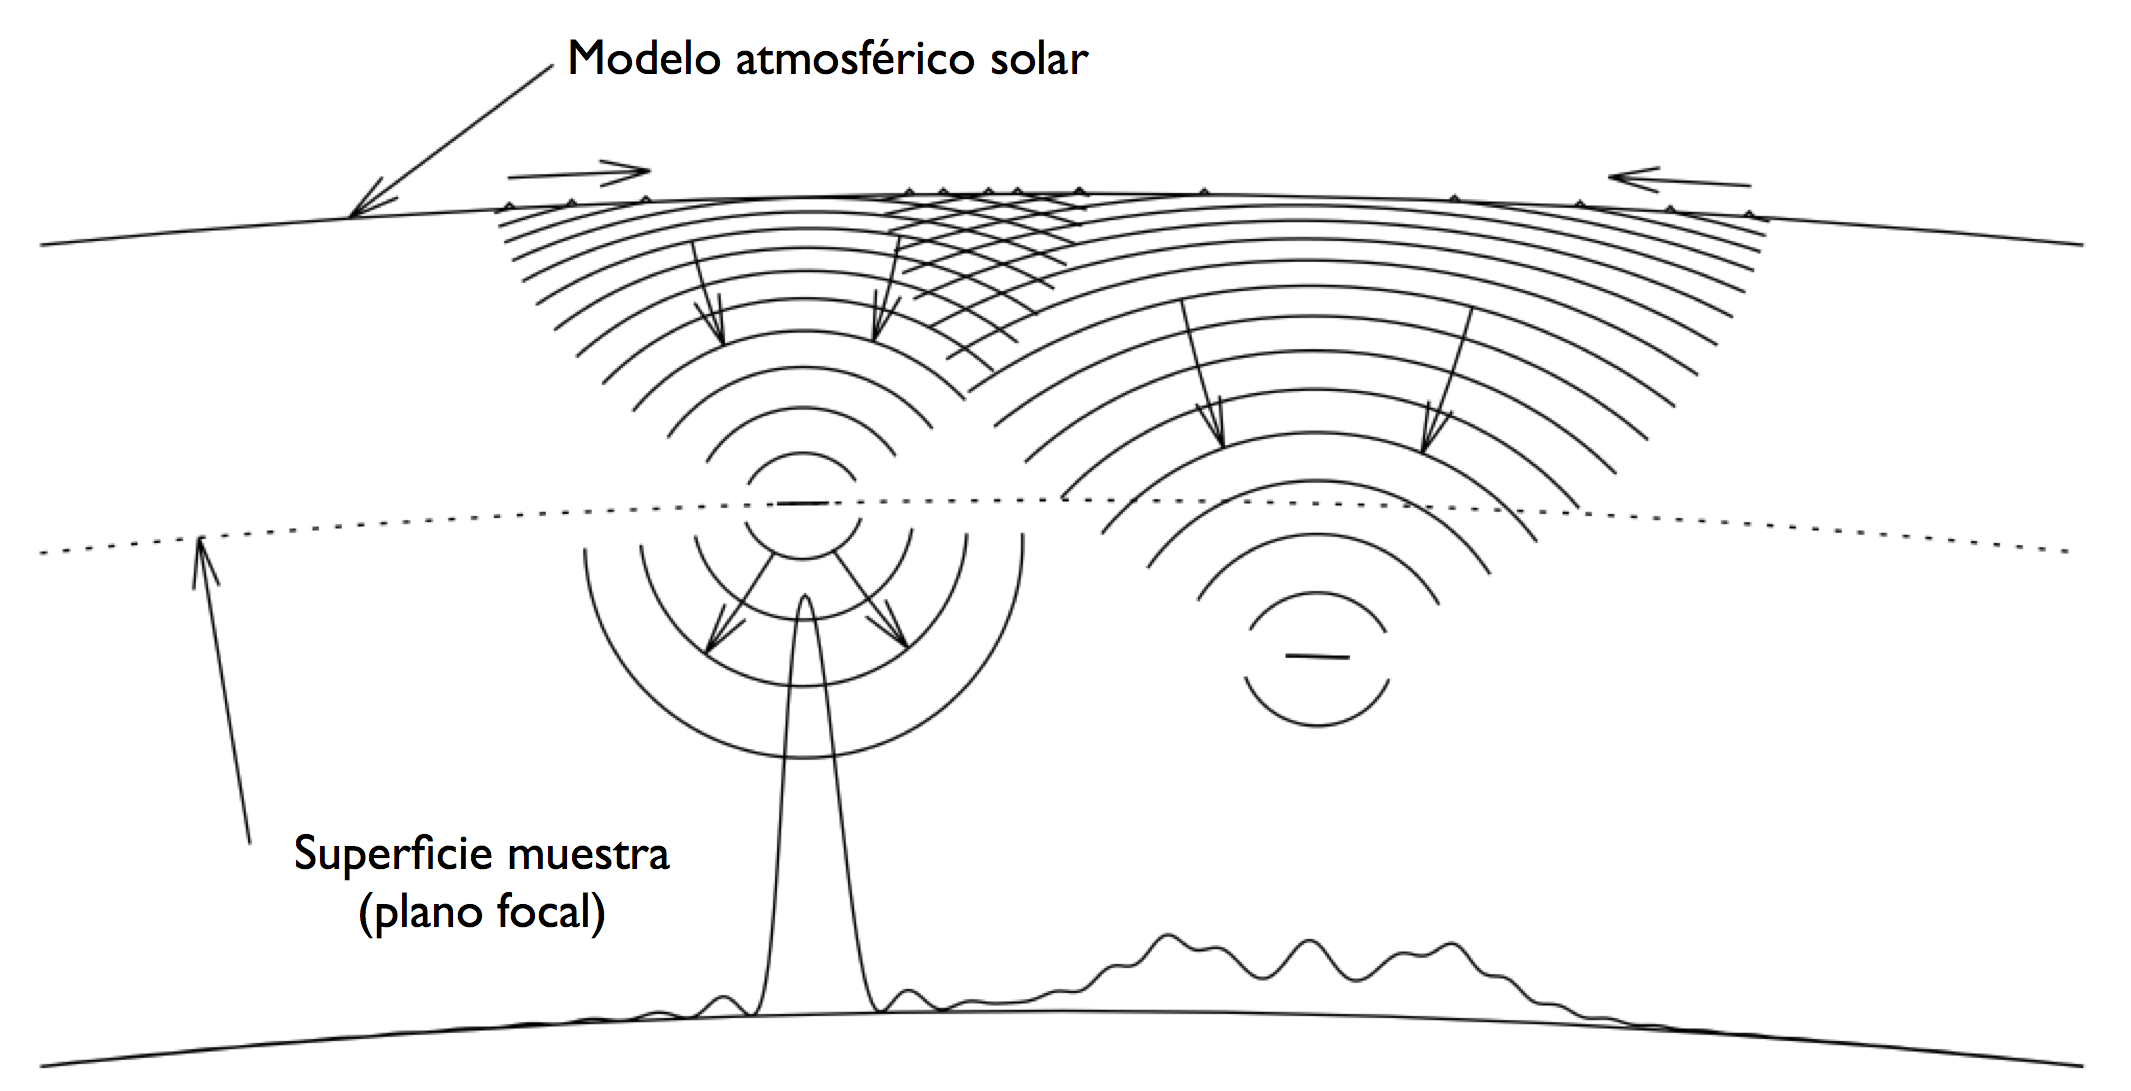
\includegraphics[width=0.51\textwidth]{acustico.png}
\caption{Representaci\'on de una regresi\'on hologr\'afica basada en un campo ac\'ustico observado en la superficie solar. Figura tomada de \cite{lb2000}.}
\label{fig:acustico}
\end{center}
\end{wrapfigure}

La holograf\'ia heliosismol\'ogica (en t\'erminos muy generales) toma las oscilaciones observadas en la superficie solar y calcula la ``imagen s\'ismica'' a cierta profundidad del Sol. Cuando esta es calculada hacia adelante en el tiempo se le llama imagen, o mapa, de {\bf egresi\'on}, mientras que cuando se calcula hacia atr\'as en el tiempo se le llama imagen, o mapa, de {
\bf ingresi\'on}. El ejercicio de diagn\'ostico b\'asico de la holograf\'ia s\'ismica consiste en aplicar una inversi\'on temporal sobre un conjunto de observaciones s\'ismicas de la superficie solar bas\'andose en un modelo computacional de la atm\'osfera solar desprovisto de fuentes, sumideros o dispersiones ac\'usticas. En general, esta t\'ecnica debe aplicarse sobre una regi\'on limitada de la superficie solar. Abusando del lenguaje propio de la \'optica a la regi\'on sobre la que se aplica este procedimiento se le llama la {\it pupila}. Una vez se define esta pupila sobre los par\'ametros de entrada del c\'odigo num\'erico y este se corre, las ahora entrantes perturbaciones ac\'usticas convergen todas juntas al punto donde se localiz\'o la fuente ac\'ustica. Si se toma una muestra de la potencia ac\'ustica en una superficie, i.e., en un ``{\it plano focal}'', a la profundidad en la que tuvo lugar la fuente ac\'ustica, el resultado ser\'a una se\~nal intensa y bien definida cuyo ancho estar\'a definido por el l\'imite de difracci\'on de la se\~nal, tal y como aparece debajo de la fuente en la parte izquierda de la figura \ref{fig:acustico}. De otro lado, si el plano focal es movido hacia arriba o hacia abajo de la profundidad a la cual se present\'o la fuente, la se\~nal en general no desaparece pero s\'i se desenfoca apreciablemente, observ\'andose un perfil difuso como el que se esquematiza en la parte baja del lado derecho de la figura \ref{fig:acustico}.\\

Considerando un medio continuo, libre de fuentes, sumideros y/o puntos de dispersi\'on, a trav\'es del cual se propaga un tren de ondas, bastar\'ia conocer la amplitud y la derivada de esta en un tiempo dado para poder extrapolar el campo ac\'ustico a trav\'es de todo el interior solar y todo tiempo por medio de la soluci\'on de la integral de Kirchhoff \citep[]{born1975}. Este tipo de procedimientos suponen una distribuci\'on {\it continua} de datos, que por obvias razones no se puede obtener de las observaciones heliosismol\'ogicas, raz\'on por la cual a pesar de que esta soluci\'on (la de la integral de Kirchhoff) pueda representar una componente significativa del campo ac\'ustico subyacente, {\bf no} debe ser considerada como una soluci\'on que de cuenta del campo ac\'ustico {\it real} ya que el medio a trav\'es del cual se propagan las ondas est\'a permeado de un mont\'on de anomal\'ias f\'isicas. De esta manera es que se encuentra la necesidad de establecer la diferencia entre el campo ac\'ustico obtenido mediante la aplicaci\'on de un modelo te\'orico de egresi\'on, $H$, y el campo ac\'ustico {\it real}, $\psi$. \cite{lindsey1997} establecen que estos dos \'ultimos campos se relacionan mediante una funci\'on de {\it Green} que da cuenta de la propagaci\'on hacia adelante y hacia atr\'as en el tiempo, $H_+(\mathbf{r},z,t)$ y $H_-(\mathbf{r},z,t)$ respectivamente.  A $H_+(\mathbf{r},z,t)$ se le suele llamar la ``{\it egresi\'on ac\'ustica}''que se relaciona con $\phi$ mediante la siguiente expresi\'on

\begin{align}\label{egresion}
H_+(\mathbf{r},z,t)=\int \, dt'\int_{a<|\mathbf{r}-\mathbf{r}'|<b}\,d^2\mathbf{r}'G_+(|\mathbf{r}-\mathbf{r}'|,z,t-t')\phi(\mathbf{r}',t'),
\end{align}

\begin{wrapfigure}[22]{r}{0.58\textwidth}
\begin{center}
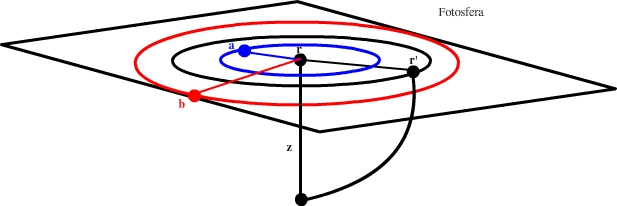
\includegraphics[width=0.56\textwidth]{egresion.jpg}
\caption{Figura que esquematiza la pupila usada en la t\'ecnica de holograf\'ia ac\'ustica sobre la superficie del Sol, en donde se resalta que se usa una pupila anular con radio interior $a$ (azul) y radio exterior b (rojo). Adem\'as que el mapa de egresi\'on es calculado sobre el punto $\mathbf{r}$ cuando las perturbaciones son vistas a lo largo de la circunferencia de radio $\mathbf{r}'$. Seg\'un esta t\'ecnica la fuente ac\'ustica se encuentra a una profundidad $z$ y la trayectoria del frente de onda es una curva debido al cambio de densidad del medio por el cual ella se propaga.}
\label{fig:egresion}
\end{center}
\end{wrapfigure}

\noindent en donde $G_+$ es la funci\'on de {\it Green} que expresa c\'omo una perturbaci\'on registrada en un punto transitorio \'unico en $(\mathbf{r},z,t)$, en el interior solar, se propaga hacia las capas m\'as externas hasta alcanzar la superficie en donde se registra el frente de onda viajero en $(\mathbf{r}',0,t')$. Por otra lado, la {\it ingresi\'on ac\'ustica}, $H_-$, es la inversi\'on temporal de la {\it egresi\'on ac\'ustica} $H_+$. Esta {\it ingresi\'on} da cuenta de las ondas que de manera coherente convergen todas juntas a un mismo punto focal en $(\mathbf{r},z)$. La {\it ingresi\'on} puede ser calculada si en la ecuaci\'on \ref{egresion} se usa como factor integrante la funci\'on de {\it Green} 

$$
G_-(|\mathbf{r}-\mathbf{r}'|,z,t-t').
$$

\noindent Esta funci\'on de {\it Green}, m\'as conocida como la funci\'on {\bf iconal} de {\it Green}, que solo depende de la direcci\'on radial gracias a la suposici\'on de simetr\'ia acimutal que se presenta en la superficie solar (cuando se habla de su estructura), puede ser descrita como un producto entre una funci\'on delta y una funci\'on $f$ que da cuenta del decremento de la amplitud de la perturbaci\'on a medida que se propaga:

\begin{align}
G_+(|\mathbf{r}-\mathbf{r}'|,z,t-t')=\delta[(t-t')-T(|\mathbf{r}-\mathbf{r}'|,z)]f(|\mathbf{r}-\mathbf{r}'|,z),
\end{align}

\noindent donde $T$ es el tiempo transcurrido entre la generaci\'on del pulso y la llegada del frente de onda al punto $\mathbf{r}'$ sobre la superficie visible del Sol. Esta representaci\'on caracteriza la din\'amica ac\'ustica del modelo solar en el que se construye una regresi\'on ac\'ustica mediante el uso de las observaciones helios\'ismicas. La holograf\'ia s\'ismica computacional ha sido desarrollada como una t\'ecnica de diagn\'ostico muy flexible de manera tal que {\bf no} est\'e restringida a un modelo de atm\'osfera solar particular. En este sentido, la funci\'on de {\it Green} puede alejarse considerablemente de lo que ser\'ia el interior solar ac\'ustico real y sin embargo seguir proporcionando im\'agenes de muy alta calidad y \'utiles para diagnosticar la ubicaci\'on de la fuente s\'ismica.\\


En aras de calcular la potencia ac\'ustica de egresi\'on \citet{lb2000} proponen hacer el c\'alculo de la ecuaci\'on (\ref{egresion}) en el dominio de las frecuencias y el n\'umero de onda; \'esto con el fin de eliminar las integraciones en el anillo y trabajar m\'as bien en forma operacional:

\begin{align}
\hat{H}_+(\mathbf{k},z,\nu)=\hat{G}_+(|\mathbf{k}|,z,\nu)\hat{\psi}(\mathbf{k},\nu),
\end{align}

\noindent donde $\hat{H}_+$, $\hat{G}_+$ y $\hat{\psi}$ son las {\it transformaciones de Fourier} en espacio y tiempo de $H_+$, $G_+$ y $\psi$, respectivamente. En este cambio se trabaja con los modos normales de oscilaci\'on ac\'ustica cuyas proyecciones sobre la superficie solar  (en la aproximaci\'on de un plano horizontal) resultan ser simplemente ondas planas viajeras. De aqu\'i la importancia de que en esta t\'ecnica, antes de entrar a aplicar la holograf\'ia ac\'ustica sobre los datos crudos reales, sea necesario realizar una proyecci\'on del disco solar que preserve las distancias verdaderas entre dos puntos contenidos en la superficie solar. Una descripci\'on detallada de esta t\'ecnica se encuentra en \cite{lindsey1997,lb2000}.

\subsection*{Proyecci\'on Postel}
\addcontentsline{toc}{subsection}{Proyecci\'on Postel}


Como vimos en la secci\'on anterior, particularmente cuando nos referimos a la figura \ref{fig:egresion}, se tiene un centro y diferentes se\~nales que arriban a la superficie desde profundidades diversas. Ahora bien, esto lo observamos en un plano de imagen; sin embargo, al Sol lo podemos suponer esf\'erico, y por lo tanto, necesitamos hacer una proyecci\'on de la descripci\'on de las se\~nales estudiadas  en un plano de imagen, si bien provienen de una superficie (solar) curva. A este tipo de proyecci\'on se le conoce en la literatura como {\it proyecci\'on azimutal equidistante} o {\it proyecci\'on Postel} por aquello de que fue usada por {\it Guillaume Postel} en la contrucci\'on de algunos mapas geogr\'aficos en 1581 \citep[]{snyder1926}. Este procedimiento consiste en generar la proyecci\'on de diversos puntos ubicados sobre la superficie esf\'erica, en un plano tangente a la esfera en el punto {\bf P}, como  se muestra en la figura \ref{fig:postel}, de manera que con respecto a este punto {\bf P} se preservan tanto las distancias como los \'angulos entre los puntos ubicados a lo largo de circunferencias conc\'entricas\footnote{Este tipo de proyecci\'on es el que se usa en el globo terrestre que se ha establecido como emblema de la {\it Organizaci\'on de las Naciones Unidas}.} en {\bf P}. 

% Comentario: Averiguar si la proyecci�n Postel es una proyecci�n CONFORME: S� lo es


La construcci\'on de la proyecci\'on Postel se lleva a cabo fijando un punto sobre la superficie solar de coordenas heliogr\'aficas $\theta$, $\varphi$ de manera que las coordinas sobre el mapa plano de todos los otros puntos se hallan mediante 

\begin{align}\label{eq:postel}
\left\{
\begin{array}{c l}      
    X'_p & =\theta'\cos\varphi'\\
    Y'_p & =\theta'\sin\varphi'
\end{array}\right.,
\end{align}

\noindent en donde $\theta'$, $\varphi'$ son unas coordenadas esf\'ericas tales que deben satisfacer que $P$ est\'e en uno de los polos y que se relaciones con $\theta$, $\varphi$ mediante el siguiente conjunto de ecuaciones:

\begin{align}\label{eq:transform}
\left\{
\begin{array}{cl}
\cos\theta'\sin\varphi'&=\cos\theta\sin(\varphi-\varphi_0)\\
\sin\theta'&=-\cos\theta\sin\theta_0\cos(\varphi-\varphi_0)+\sin\theta\cos\theta_0\\
\cos\theta'\cos\varphi'&=\cos\theta_0\cos\theta\cos(\varphi-\varphi_0)+\sin\theta_0\sin\theta
\end{array}\right.,
\end{align}

\noindent siendo $\theta_0$ y $\varphi_0$ las coordenadas del punto $P$ en las antiguas coordenadas esf\'ericas \citep[]{pearson1977}.


\begin{figure}[ht!]
\centering
\subfloat[]{
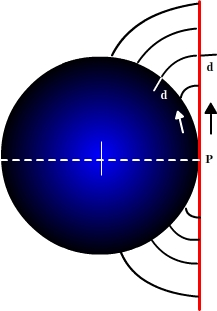
\includegraphics[width=0.2\textwidth]{postela.jpg}}
\subfloat[]{
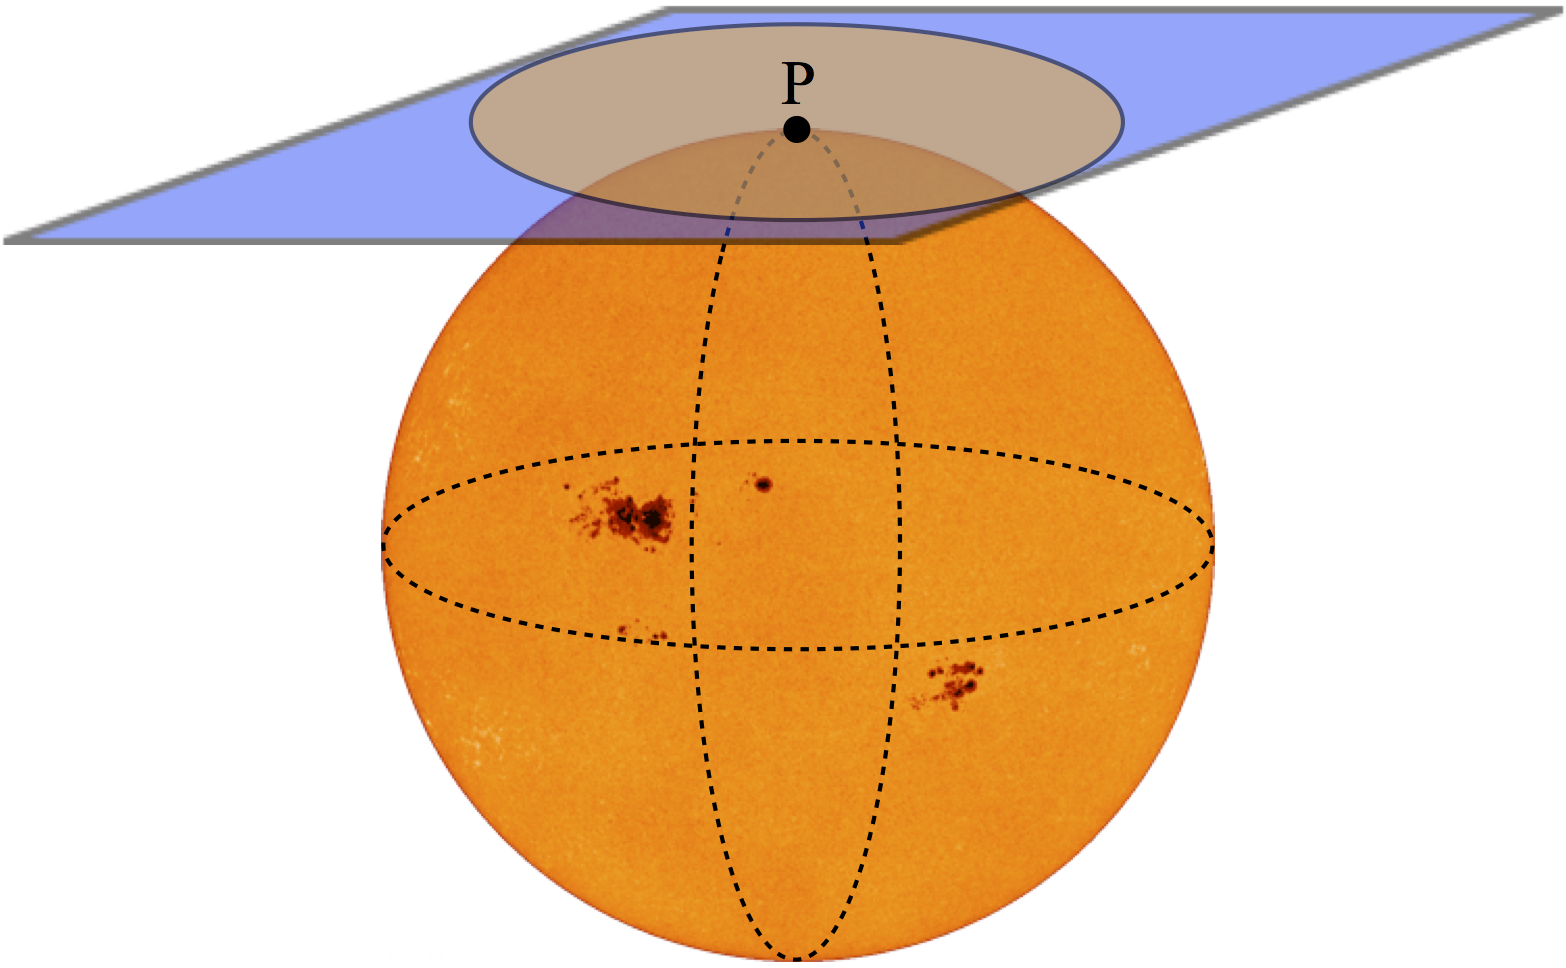
\includegraphics[width=0.37\textwidth]{postelb.png}}
\subfloat[]{
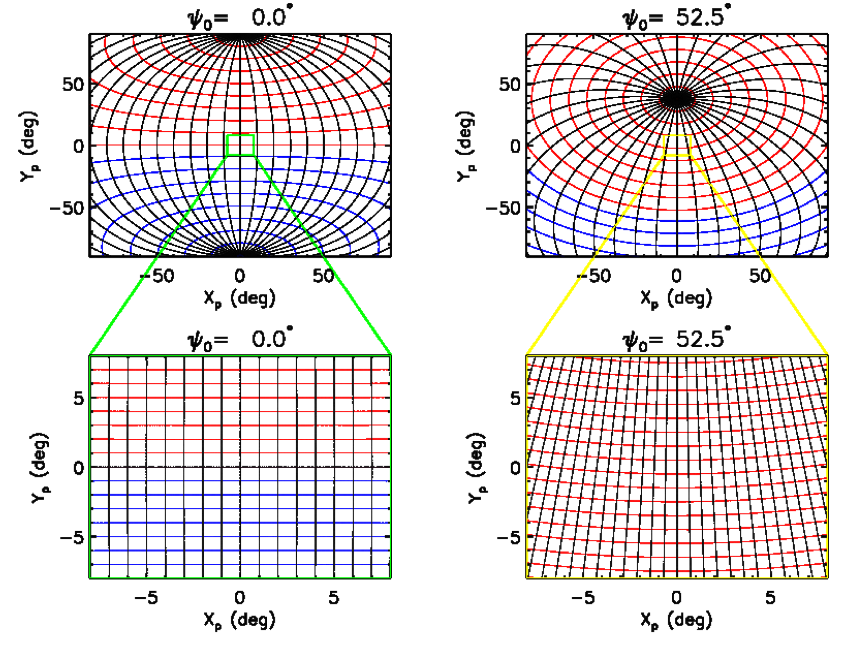
\includegraphics[width=0.37\textwidth]{postelc.png}}
\caption{Conjunto de figuras que esquematizan la proyecci\'on {\it Postel}. (a) Vista en perspectiva de una superficie completamente esf\'erica (azul) que se proyecta sobre un plano (rojo). En este los trazos en negro representan la proyecci\'on de cada uno de los puntos de la esfera sobre el plano y se observa claramente c\'omo las distancias se conservan a lo largo de una l\'inea trazada en direcci\'on radial con centro en el punto P. (b) La proyecci\'on {\it Postel} de la superficie solar centrada en un punto P ubicado en uno de los polos helioc\'entricos. (c) Representaci\'on de los meridianos y paralelos helioc\'entricos en una proyecci\'on azimutal equidistante a una latitud de $0^\circ$ (arriba a la izquierda) y a una latitud de $52.2^\circ$ (arriba a la derecha). Un acercamiento al punto centrado se muestra en las im\'agenes de abajo respectivamente. N\'otese que las coordenadas que se manejan sobre el mapa son $X_p$ y $Y_p$. Las figuras (c) son tomadas de \citet{corbard2003}.}
\label{fig:postel}
\end{figure}


\subsection*{Sismicidad asociada a las fulguraciones solares}
\addcontentsline{toc}{section}{Sismicidad asociada a las fulguraciones solares}
 \label{sec:sismicidad}

El inter\'es constante por entender los procesos mediante los cuales la energ\'ia es transportada, almacenada y (posteriormente) liberada en las fulguraciones solares se ha convertido en uno de los problemas abiertos m\'as interesantes que en las \'ultimas d\'ecadas han ocupado a los astrof\'isicos solares.\\  

Con el advenimiento de la era espacial en la astronom\'ia, es mucha la informaci\'on que se ha obtenido de estos eventos explosivos y ya es bastante lo que se ha aprendido acerca de los procesos que tienen lugar en la alta atm\'osfera solar. Sin embargo, a pesar de estos grandes avances a\'un son muchas las inc\'ognitas que se tienen con respecto a los efectos que tienen las fulguraciones sobre las partes m\'as profundas a la fotosfera. \cite{wolff72} lanz\'o la primera propuesta reportada de que estas explosiones solares podr\'ian impactar directamente el interior solar, pero fue solo hasta un par de d\'ecadas despu\'es cuando por primera vez se pudo tener registro ver\'idico de este fen\'omeno en forma de ``{\it sun-quakes}'' o sismos solares \citep[]{kz1998}, visibles como ondas expansivas circulares que se propagan sobre la superficie solar, como se representa en la figura \ref{fig:sunquake}. Trabajos posteriores han mostrado una correlaci\'on alta (temporal y espacial) entre la aparici\'on de estas ondulaciones y una emisi\'on fuerte en rayos-X \citep[]{dl2005}, luz blanca \citep[]{detal2006,metal2006b,mo2007} y cambios permanentes en la topolog\'ia del campo magn\'etico local \citep[]{h2000,schunker2005,metal2006a}. Al leer estos trabajos se evidencia que, debido a la heterogeneidad de las evidencias observacionales obtenidas, han surgido toda una variedad de propuestas que tratan de dar una explicaci\'on plausible a la aparici\'on de estas se\~nales s\'ismicas observadas en algunas regiones activas haciendo uso de diferentes procesos f\'isicos. La mayor\'ia de estas propuestas  est\'an enmarcadas en alguno(s) de los siguientes mecanismos:\\

{\bf Ondas de choque:} Durante la liberaci\'on de energ\'ia magn\'etica en una fulguraci\'on se presenta movimiento de material coronal. Algo de este material es eyectado hacia el espacio interplanetario mientras que otra fracci\'on se mueve hacia la fotosfera. Este material entrante se termaliza  en la corona pero una parte de este alcanza a llegar a la cromosfera donde el rayo de part\'iculas pierde su energ\'ia produciendo una emisi\'on en rayos-X duros y calentando el material que est\'a a su alrededor que m\'as tarde se enfr\'ia emitiendo en rayos-X blandos y en H$\alpha$. \cite{kz1995,kz1998} propusieron que esa interacci\'on entre las part\'iculas entrantes y el plasma cromosf\'erico act\'ua como detonante de una onda de choque que se propaga hacia el interior solar induciendo ondas subfotosf\'ericas. Eventualmente estas ondas alcanzan la fotosfera, despu\'es de un proceso de refracci\'on en el interior solar gobernado por el aumento en la densidad con el aumento en la profundidad y, por lo tanto, un cambio en el valor de \'indice refraci\'on $n$, y entonces son vistas como ondas circulares expansivas sobre un mapa de diferencias Doppler.\\

{\bf Backwarming radiation:} En espa\~nol ser\'ia algo as\'i como ``sobrecalentamiento por radiaci\'on''. El hecho de que la densidad en la cromosfera aumente con la profundidad plantea algunas interrogantes con respecto a la viabilidad de la anterior propuesta, ya que la onda de choque podr\'ia ser absorbida r\'apidamente a causa del cambio dr\'astico del medio en el que se propaga y de esa manera jam\'as alcanzar\'ia la fotosfera. Las observaciones hechas por el grupo de {\it Donea, Lindsey, Cally, Moradi, Besliou, Mart\'inez-Oliveros} \citep[]{dl2005,metal2007} han mostrado que una gran cantidad de {\it sunquakes} han estado fuertemente correlacionados con un aumento apreciable en la emisi\'on de luz blanca en el sector.\\

El mecanismo de generaci\'on de {\it sunquakes} debido al ``sobrecalentamiento por radiaci\'on'' fue propuesto por primera vez por el grupo de \cite{machado1989}. En este mecanismo se plantea que los electrones altamente energ\'eticos junto con los fotones asociados a los rayos-X alcanzan la fotosfera y r\'apidamente calientan el material produciendo un aumento considerable en la emisi\'on de luz blanca. Se supone que es la presi\'on de radiaci\'on involucrada en este proceso la responsable de generar ondas que se propagan en el interior solar y que posteriormente son vistas en la fotosfera. Para que se presente este tipo de din\'amica se necesita que una gran cantidad de energ\'ia act\'ue como detonador del sismo. Las fulguraciones fuertes, como lo son las tipo X o las tipo X10, almacenan la suficiente energ\'ia como para que en su liberaci\'on esta hip\'otesis sea un escenario viable en el proceso de generaci\'on de la fuente s\'ismica; sin embargo, hace suponer la imposibilidad de observar se\~nales sismicas asociadas a fulguraciones m\'as d\'ebiles, lo cual, como sabemos, ha sido refutado por trabajos como el de \cite{mo2007}.\\

%OJO COMPLEMENTAR CON LA AMIGA DEL PROFE: VALENTINA! :P 

{\bf Colisi\'on directa de part\'iculas:} Algunas observaciones (\citep[]{dl2005,zz2007}) han mostrado una fuerte correlaci\'on entre la sismicidad de regiones activas y la emisi\'on en rayos gamma. Este tipo de emisi\'on es producida por protones altamente energ\'eticos, acelerados desde el punto de reconexi\'on del evento de fulguraci\'on, al colisionar con el material fotosf\'erico (se cree que es en la fotosfera y no en la cromosfera debido a la densidad alta necesaria para producir el frenado del haz de protones incidentes). La energ\'ia y el momentum llevados por los protones es suficiente para dar cuenta del exceso visto en luz blanca. Este mecanismo puede generar una presi\'on de radiaci\'on y un trabajo mec\'anico como para ser un mecanismo responsable de producir una fuente s\'ismica y posteriormente dar pie a la propagaci\'on de las ondas ac\'usticas. Los detalles de este mecanismo est\'an ampliamente explicados en \cite{zz2007}. El argumento m\'as fuerte que va en contra de esta propuesta es la visualizaci\'on de actividad s\'ismica en fulguraciones que no tienen evidencia de un gran n\'umero de protones acelerados, es decir, con ausencia de emisi\'on en rayos-gamma \citep[]{mo2007}.\\

{\bf McClymont jerk (variaci\'on del campo magn\'etico):} Este mecanismo es discutido ampliamente en \cite{Hudson2008}. En este se plantea que son los cambio en la topolog\'ia y en la intensidad del campo magn\'etico a lo largo de una fulguraci\'on, los responsables de la generaci\'on del sismo solar.\\

\begin{wrapfigure}[24]{r}{0.55\textwidth}
\begin{center}
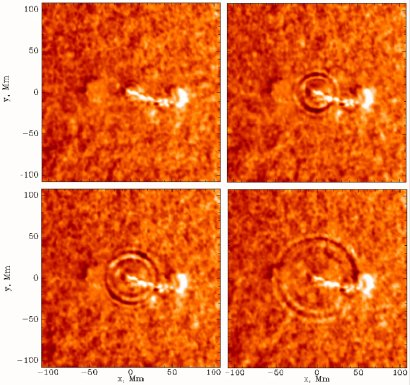
\includegraphics[width=0.5\textwidth]{sunquake.jpg}
\caption{Din\'amica de las ondas expansivas asociadas al primer sismo solar ocurrido el 9 de Julio de 1996 y reportado por \cite{kz1998}.}
\label{fig:sunquake}
\end{center}
\end{wrapfigure}

Las fulguraciones son eventos din\'amicos que involucran cambios significativos en la configuraci\'on del campo magn\'etico coronal. La consecuencia m\'as inmediata es el colapso del bucle coronal hacia una configuraci\'on m\'as estable (m\'as horizontal). Si este proceso se lleva a cabo con la suficiente rapidez podr\'ia llegar a generar trabajo mec\'anico sobre la superficie solar, y por ende, podr\'ia ser un buen candidato en la consideraci\'on de la generaci\'on de la fuente de se\~nales ac\'usticas.  Esta din\'amica posible fue bautizada como el {\it McClymont jerk} por \cite{Hudson2008}. Lo interesante de esta propuesta es que se aleja de hip\'otesis de que es la interacci\'on de las part\'iculas incidentes el detonante de ondas s\'ismicas; sin embargo, a\'un hoy en d\'ia es un tema de \'algida discusi\'on en los diferentes eventos que se celebran en torno a estos temas.\\

?`Cu\'al de todas estas propuestas resulta ser la m\'as eficiente y adecuada para describir el proceso mediante el cual se deposita la energ\'ia necesaria para la generaci\'on del sismo? Es una pregunta que es muy dif\'icil de responder y que solo las observaciones, cada vez de mayor calidad, podr\'an dar luz al respecto. Quiz\'as todo se trate de una soluci\'on salom\'onica en la que dependiendo de las condiciones f\'isicas que definen la prefulguraci\'on uno o varios de estos mecanismos pueden dominar el efecto de generar la fuente ac\'ustica. En el desarrollo que se presenta aqu\'i trabajamos sobre la hip\'otesis de que es justamente el jet de part\'iculas incidentes el mecanismo sobre el cual se podr\'ia asociar la generaci\'on de uno de estos {\it sunquakes}; pero hemos de establecer la forma en que se deben acelerar estas part\'iculas (electrones) que en nuestro caso ser\'a siguiendo una din\'amica estoc\'astica.\\

\section*{M\'etodo de limpieza de observaciones hechas desde tierra}
\addcontentsline{toc}{section}{M\'etodo de limpieza de observaciones hechas desde tierra}

Despu\'es de que \cite{kz1998} reportaran el primer ``{\it tsunami}'' solar, muchos otros cient\'ificos centraron su atenci\'on en tratar de encontrar m\'as eventos como este asociados a fulguraciones solares muy energ\'eticas, con el \'animo de tratar de dar una explicaci\'on f\'isica a la generaci\'on de la fuente s\'ismica mediante un acercamiento m\'as bien estad\'istico. En esta direcci\'on, \cite{detal2006a} desarrollaron una prospecci\'on sobre las fulguraciones m\'as energ\'eticas que ocurrieron durante el m\'aximo del ciclo solar 23 encontrando cerca de 13 eventos s\'ismicos. Para hacer esta inspecci\'on, ellos hicieron uso de las im\'agenes obtenidas por la red de telescopios en tierra GONG++ y aplicaron la t\'ecnica de {\it holograf\'ia heliosismol\'ogica} descrita anteriormente. Sin embargo, y como es bien conocido por todos los astr\'onomos observacionales, el hacer observaciones desde tierra implica tener que considerar los efectos que  tiene la turbulencia atmosf\'erica sobre las im\'agenes obtenidas. En el caso solar esto no es una excepci\'on, y m\'as teniendo en cuenta que para poder distinguir las ondas que se propagan sobre la superficie solar se necesita una resoluci\'on espacial alta en las im\'agenes, de al menos unos tres segundos de arco, adem\'as de un alto contraste regido por la raz\'on se\~nal ruido que para el caso de los {\it sunquakes} es del orden de $\sim 10$, en im\'agenes filtradas por frecuencia, t\'ipicamente centradas en 5 mHz con un pasabandas de 2 mHz \citep[]{kz2006c}. Esta red de observatorios nos ha provisto de fotogramas, Dopplergramas y magnetogramas del Sol calmo de calidad muy alta, pero la limitaci\'on que tiene a la hora de analizar im\'agenes de regiones activas es justamente la consecuencia de la turbulencia atmosf\'erica sobre la imagen final integrada en un minuto de tiempo (imperfecciones por ``{\it seeing}''). En Sol calmo las variaciones debidas a la turbulencia no son percibidas apreciablemente pues no hay una se\~nal fuerte sobre la que puedan influir de sobremanera. Sin embargo, cuando hay un gradiente alto en las intensidades registradas, como es el caso de una regi\'on activa, se genera un ruido que altera las se\~nales s\'ismicas que se quieren analizar haciendo que el implementar los m\'etodos heliosismol\'ogicos sobre las regiones activas se vuelva algo impr\'actico a primera vista.

\subsection*{Algoritmo param\'etrico de correci\'on por turbulencia (PASCAL)}
\addcontentsline{toc}{subsection}{Algoritmo param\'etrico de correci\'on por turbulencia (PASCAL)}

\cite{Lindsey2008} han ideado un algoritmo que aplicado sobre las im\'agenes terrestres obtenidas con GONG++, es capaz de distinguir una se\~nal s\'ismica sobre el ruido de la imagen producto de la turbulencia. Este m\'etodo es aplicable a observaciones que han sido integradas por un periodo de tiempo largo comparado con el tiempo caracter\'istico del ``{\it seeing}'' ($\sim 10$ ms). Teniendo en cuenta que la cadencia de los instrumentos de esta red es de {\bf un minuto}, este m\'etodo resulta ser adecuado a fin de ``limpiar'' las im\'agenes crudas que salen del telescopio siempre y cuando se tenga un excelente control sobre el guiado (``{\it traking}'') de las im\'agenes, lo cual para el caso del Sol se puede hacer muy bien con ayuda del limbo solar.\\

Aunque este m\'etodo de limpieza ha sido aplicado a una cantidad apreciable de estudios heliosismol\'ogicos \citep{detal2006,mo2008a,mo2008b,mo2008d,martinez-oliveros2009,matthews2011,zharkov2011}, no se le ha acu\~nado a\'un un t\'ermino para referirse a este m\'etodo en la literatura. Se ha aprovechado este trabajo y un art\'iculo que est\'a en preparaci\'on para postular el nombre sugerido por {\it Charles Lindsey}: {\bf PASCAL} que son las siglas en ingl\'es de ``{\it {\bf PA}rametric {\bf S}mearing {\bf C}orrection {\bf AL}gorithm}''. Este m\'etodo supone que despu\'es de un minuto de integraci\'on (que es la cadencia t\'ipica de los instrumentos de GONG) las perturbaciones atmosf\'ericas pueden ser consideradas como isotr\'opicas, cosa que facilita mucho el planteamiento de un tratamiento pr\'actico sobre las im\'agenes y que no est\'a lejos de la realidad pues un minuto de integraci\'on significa unas dos mil variaciones de la imagen que se registra debido al {\it seeing} atmosf\'erico.\\

Supongamos que $I(\mathbf{r})$ representa la intensidad real del objeto sobre la imagen cruda que se obtiene del instrumento, mientras que $I'(\mathbf{r})$ representa la intensidad observada (es decir la imagen real convolucionada con el ruido atmosf\'erico integrado en un minuto). $S(\mathbf{r})$ representar\'a la funci\'on (isotr\'opica) de la perturbaci\'on atmosf\'erica. Todas estas cantidades dependen de $\mathbf{r}$ que es la ubicaci\'on de un punto sobre la imagen cruda. De esta manera se tiene que

\begin{align}
I'&=(S*I)\\
SI&=(S*I).
\end{align}

Este operador de perturbaci\'on,$S$, debe contener los efectos que la atm\'osfera tiene sobre las im\'agenes en su totalidad.

\begin{wrapfigure}[30]{l}{0.65\textwidth}
\begin{center}
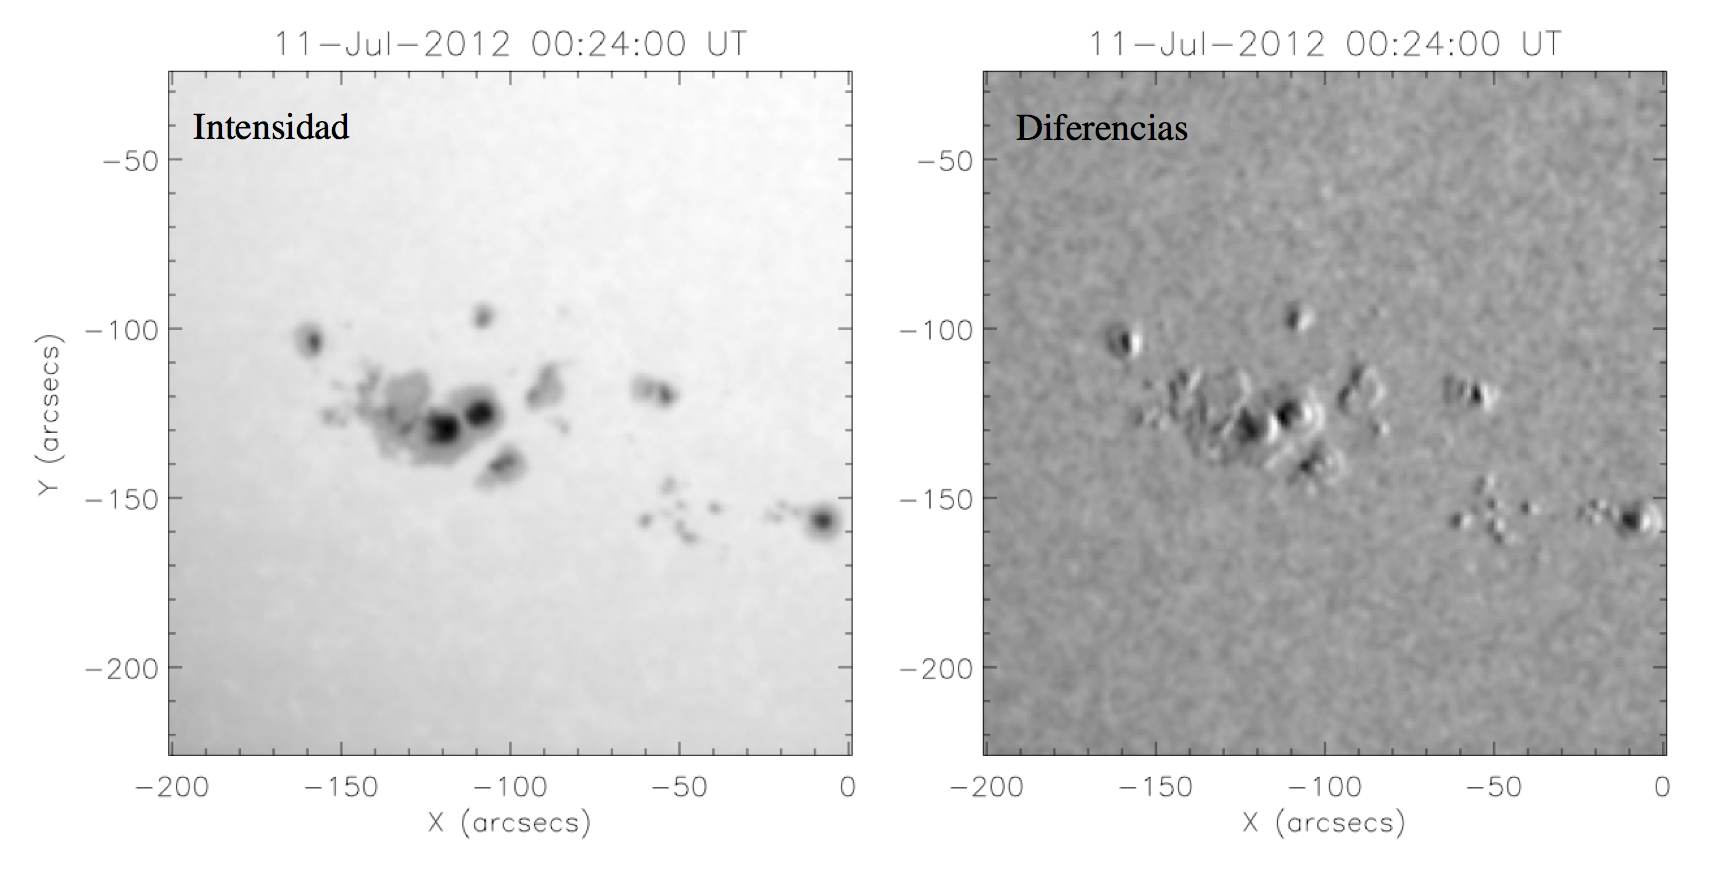
\includegraphics[width=0.64\textwidth]{Diff_gong.png}
\caption{Regi\'on activa NOAA 11520 que fue visible desde tierra desde el 6 de Julio hasta el 17 de Julio de 2012. Esta mancha solar se caracteriz\'o por ser tan grande que fue posible observarla con los filtros adecuados pero sin instrumentos de aumento en el marco de lo que fue la {\it International Summer School - Solar Astrophysics: Modern Trends and Techniques} realizada en Bogot\'a. {Izquierda}: Imagen en intensidad tomada por GONG++ el 11 de Julio de 2012 a las 00:24 UT. {Derecha}: Diferencia entre la imagen de la izquierda y la registrada por GONG++ al minuto siguiente (00:25 UT). Es claramente apreciable como los efectos de {\it seeing} atmosf\'erico tienen mayor incidencia sobre las regiones activas que sobre el Sol-calmo. Im\'agenes de diferencias, como la que se muestra aqu\'i, son usada en el m\'etodo {\bf PASCAL} para caracterizar las perturbaciones presentes en la im\'agen minuto a minuto.}
\label{fig:diff_gong}
\end{center}
\end{wrapfigure}

Estos efectos se pueden representar en dos din\'amicas b\'asicas. Una traslaci\'on estoc\'astica de la regi\'on de inter\'es, que aqu\'i se representa mediante un vector  desplazamiento $\vec{\alpha}$ definido sobre el plano de la im\'agen, y una deformaci\'on (difusi\'on) de la imagen debido a la diferencia de los caminos \'opticos de los rayos provenientes del objeto de ciencia extendido, que en nuestro caso es el disco solar, y que supondremos se caracteriza por un par\'ametro $\beta$. De esta manera el operador $\hat{S}$ se puede expresar como la suma de un t\'ermino convetivo y un t\'ermino difusivo que act\'uan sobre la se\~nal real:

\begin{align}
\hat{S}(\mathbf{r})=\hat{1}-\vec{\alpha}\cdot\vec{\nabla} + \beta\nabla^2
\end{align}

Para poder aplicar el m\'etodo se hacen dos suposiciones adicionales: Se supone que las perturbaciones generadas sobre la imagen producto del {\it seeing} atmosf\'erico son isotr\'opicas y que el tama\~no de estas son significativamente m\'as peque\~nas que el tama\~no del objeto de ciencia. Gracias a estas suposiciones podemos agrupar el t\'ermino convectivo dentro del t\'ermino difusivo y tratar la perturbaci\'on como un efecto que act\'ua de la forma $\hat{S}=\hat{1} + \beta'\nabla^2$, de manera que aplicado sobre la imagen {\it real} tenemos:

\begin{align}\label{operadorS}
\hat{S}I(\mathbf{r})&= I + \beta'(\mathbf{r})\nabla^2I(\mathbf{r})\\
I'(\mathbf{r})&= I(\mathbf{r}) + \beta'(\mathbf{r})\nabla^2I(\mathbf{r})\\
\Delta I(\mathbf{r})&=\beta'(\mathbf{r})\nabla^2I(\mathbf{r}).
\end{align}

En un periodo de tiempo del orden de un par de horas podemos suponer que $\Delta I(\mathbf{r})=[I'(\mathbf{r})-I(\mathbf{r})]\approx [I'_{(t_i+1\,\text{min})}(\mathbf{r})-I_{t_i}'(\mathbf{r})]$, de manera que im\'agenes de la diferencia entre dos fotogramas consecutivos tomados por GONG++, como la que se muestra en la figura \ref{fig:diff_gong}, representan muy bien el t\'ermino difusivo $\beta'\nabla^2 I_{t_i}(\mathbf{r})$. El algoritmo que \cite{Lindsey2008} desarrollaron lo que hace es justamente ajustar las im\'agenes de diferencias a un laplaciano de la im\'agen precedente y calcular de esta manera los coeficientes $\beta'(\mathbf{r})$ para cada p\'ixel de la imagen de ciencia y con la cadencia del instrumento, un minuto. De esta manera la tarea se reduce a tener que resolver num\'ericamente una ecuaci\'on de {\it Poisson} en cada punto de la imagen a la cual previamente se le ha aplicado una proyecci\'on {\it Postel} para garantizar que se est\'a trabajando en un espacio homog\'eneo e isotr\'opico. Para resolver la ecuaci\'on de {\it Laplace}, \cite{Lindsey2008} aplicaron el m\'etodo de {\it diferencias finitas} inicialmente con un esquema de {\bf 5 puntos} para la descomposici\'on del {\it Laplaciano} que parece en la ecuaci\'on de {\it Poisson}. 

\subsection*{Algoritmo num\'erico para el c\'alculo del laplaciano de una funci\'on bidimensional}
\addcontentsline{toc}{subsection}{Algoritmo num\'erico para el c\'alculo del laplaciano de una funci\'on bidimensional}

\begin{wrapfigure}[24]{r}{0.5\textwidth}
\begin{center}
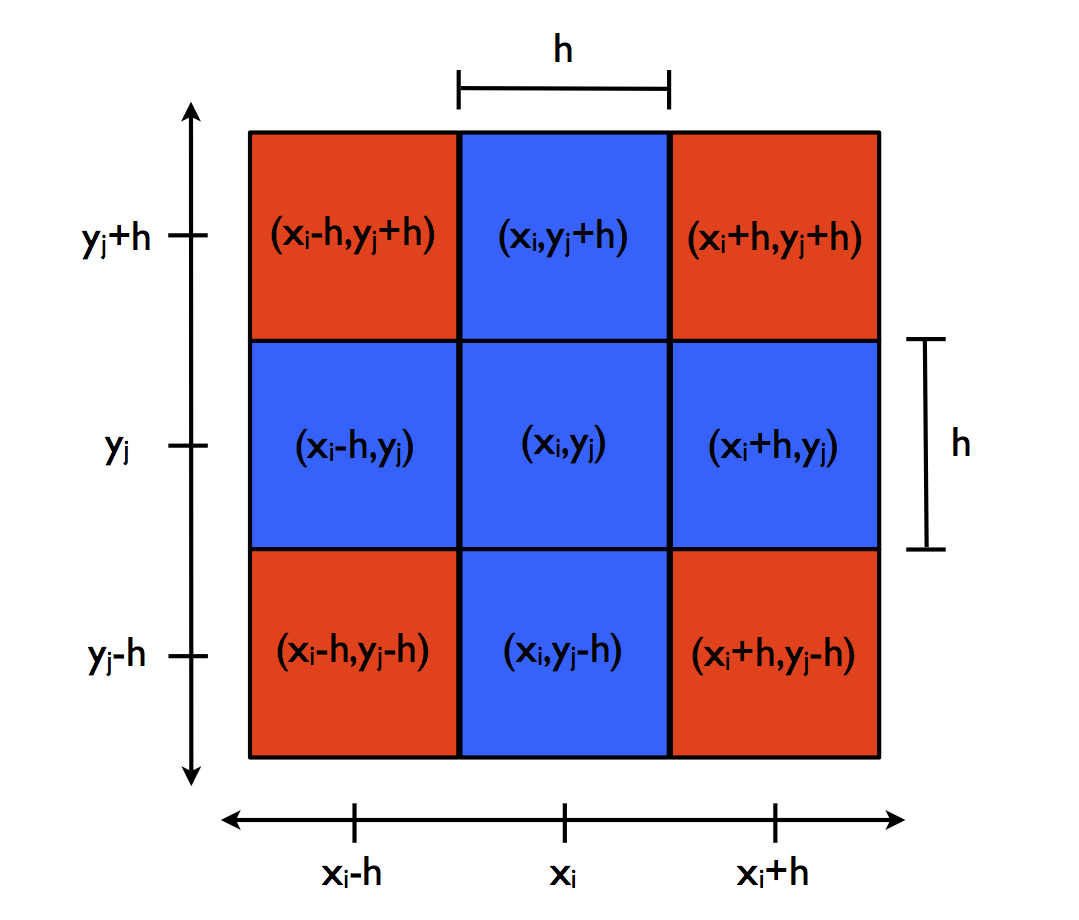
\includegraphics[width=0.52\textwidth]{9puntos.png}
\caption{Ilustraci\'on de los primeros (cuadros azules) y segundos (cuadros rojos) vecinos de una celda que pertenece a una grilla a la cual se le piensa aplicar un m\'etodo num\'erico tales como el de {\it Lattice Boltzmann} o el de diferencias finitas.}
\label{fig:9puntos}
\end{center}
\end{wrapfigure}

Modernamente las im\'agenes solares se registran en arreglos bi-dimensionales finitos de p\'ixeles en c\'amaras CCDs; usualmente, estas c\'amaras tienen escalas iguales en ambos ejes, los cuales denotamos como ejes $x$, $y$. Al trabajar sobre estos arreglos podemos expresar al laplaciano como 

\begin{align}
\nabla^2I(\mathbf{r})=\nabla^2I(x,y)\approx f(x,y),
\end{align}

\noindent en donde se define $f(x,y)=\frac{\Delta I(x,y)}{\beta'(x,y)}$, asumiendo adem\'as que las variables cartesianas $x$, $y$ son linealmente independientes. El c\'alculo num\'erico del laplaciano en un punto interior del fotograma bajo estudio tiene ocho puntos vecinos. Existen dos posibilidades sencillas del c\'alculo del laplaciano; uno que contempla los p\'ixeles en el vecindario inmediato de columna y fila, a los cuales llamaremos de aqu\'i en adelante los primeros vecinos, y que se ilustran en azul en la figura \ref{fig:9puntos}. El otro m\'etodo considera al vecindario inmediato completo, es decir, tanto los cuadros azules como rojos de la figura \ref{fig:9puntos}. Al laplaciano calculado en el primero de los casos lo llamaremos el {\it laplaciano de 5 puntos}. Este se puede expresar como:

\begin{align}\label{eq:lap5}
\nabla^2I(x_i,y_j)&\approx I(x_i+h,y_j)+I(x_i-h,y_j)\\\nonumber
&+I(x_i,y_j+h)+I(x_i,y_j-h)\\\nonumber
&-4I(x_i,y_j)=h^2f(x_i,y_j),
\end{align}

\noindent en donde $h$ es el tama\~no del lado del cuadrado de un p\'ixel que por razones de simplicidad en la implementaci\'on del m\'etodo num\'erico se tom\'o como uno. Esta forma de calcular el laplaciano es haciendo uso de los primeros vecinos del p\'ixel ubicado en $(x_i,y_j)$ obteniendo una precisi\'on de segundo orden en $h$. Si se quiere hacer este mismo c\'alculo pero incluyendo adem\'as a los segundos vecinos del p\'ixel evaluado  (cuadros rojos de la figura \ref{fig:9puntos}), entonces se procede implementando lo que se conoce como el c\'alculo del laplaciano con {\bf 9 puntos}, de forma que se tiene \citep{vooren1967}:

\begin{align}
&\nabla^2I(x_i,y_j)=f(x_i,y_j),\\\nonumber
&I(x_i+1,y_j+1)+I(x_i+1,y_j-1)+I(x_i-1,y_j+1)+I(x_i-1,y_j-1)+\\\nonumber
&+4\,[I(x_i+1,y_j)+I(x_i-1,y_j)+I(x_i,y_j+1)+I(x_i,y_j-1)]-20\,I(x_i,y_j)=6f(x_i,y_j).
\end{align}

Una vez hallados los $f(x_i,y_j)$ sobre toda la grilla, es posible determinar el valor de los $\beta'$ para cada p\'ixel mediante $\beta'(x_i,y_j,t_k)=\frac{\Delta I(x_i,y_j,t_k)}{f(x_i,y_j,t_k)}$, y de esta manera construir el operador $\hat{S}$ definido en (\ref{operadorS}) para finalmente aplicarlo como m\'etodo de limpieza a la totalidad de las im\'agenes. Todos los trabajos desarrollados hasta este momento en los que se desarrollan an\'alisis heliosismol\'ogicos usando im\'agenes de la red GONG han 

\begin{wrapfigure}[27]{r}{0.55\textwidth}
\begin{center}
\subfloat{
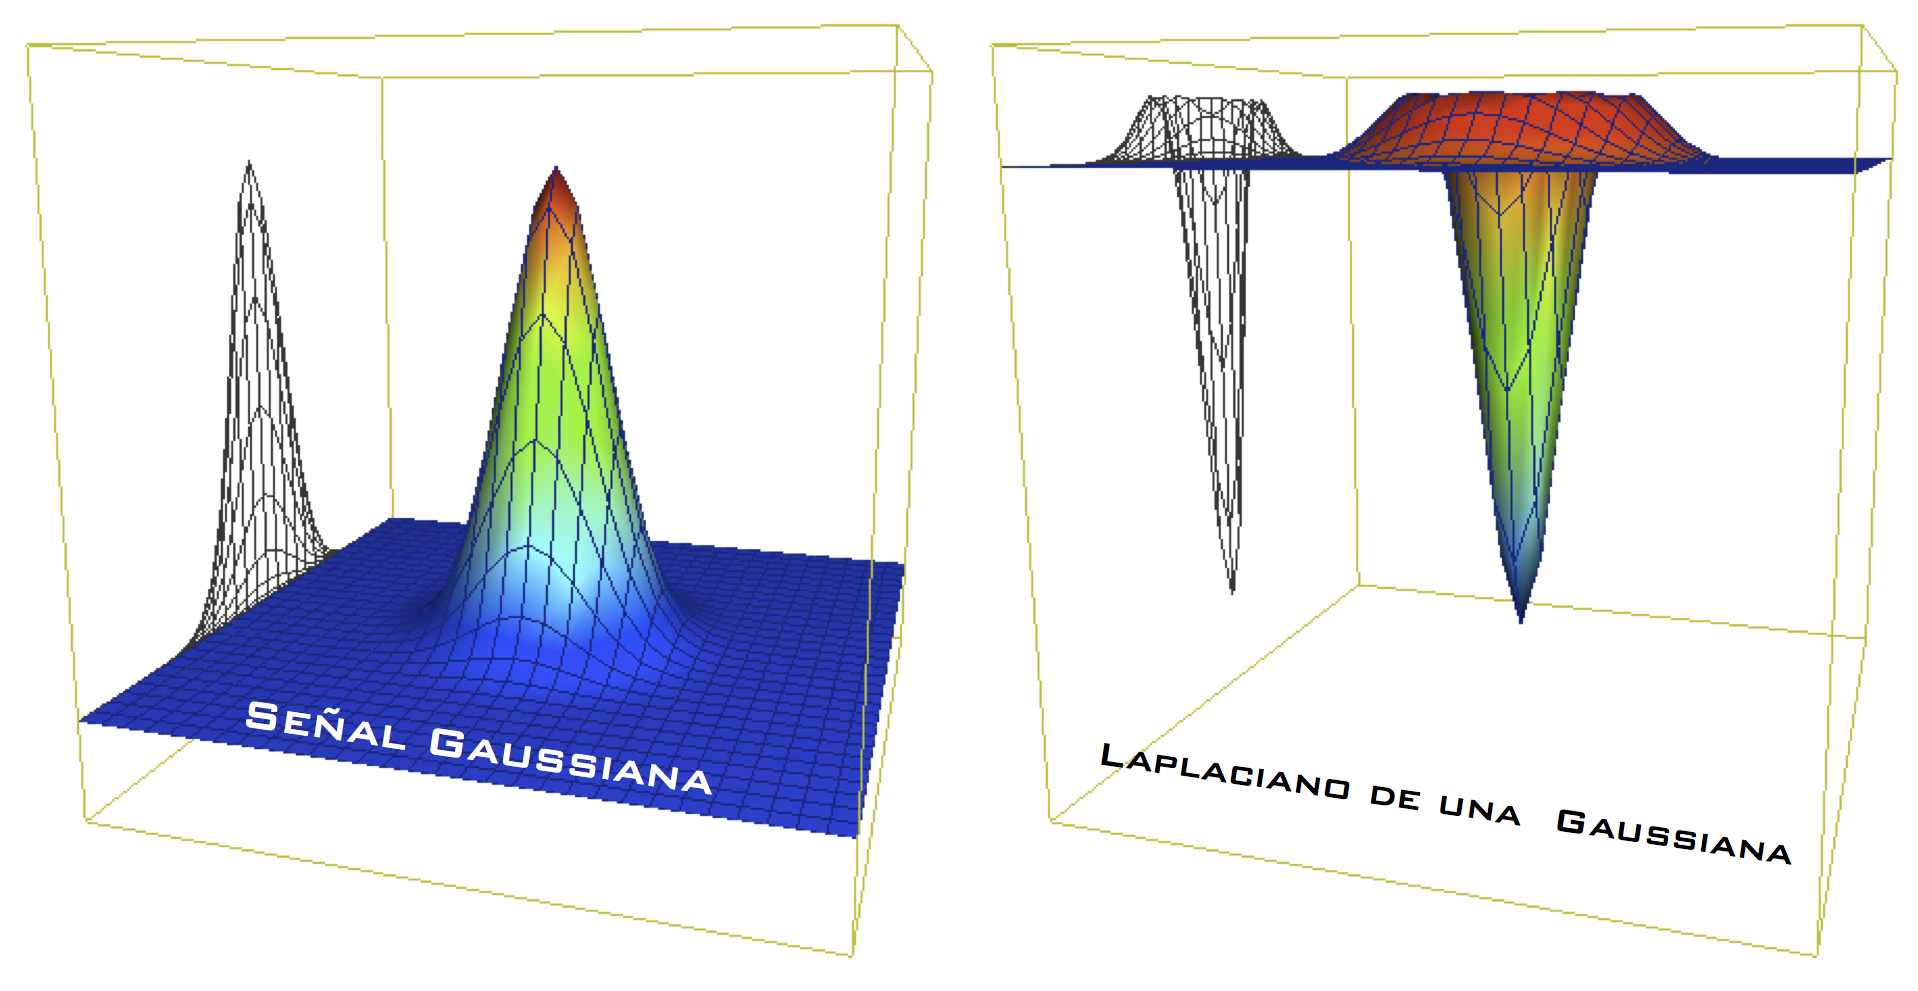
\includegraphics[width=0.55\textwidth]{gauss.png}
}\\[20pt]
\subfloat{
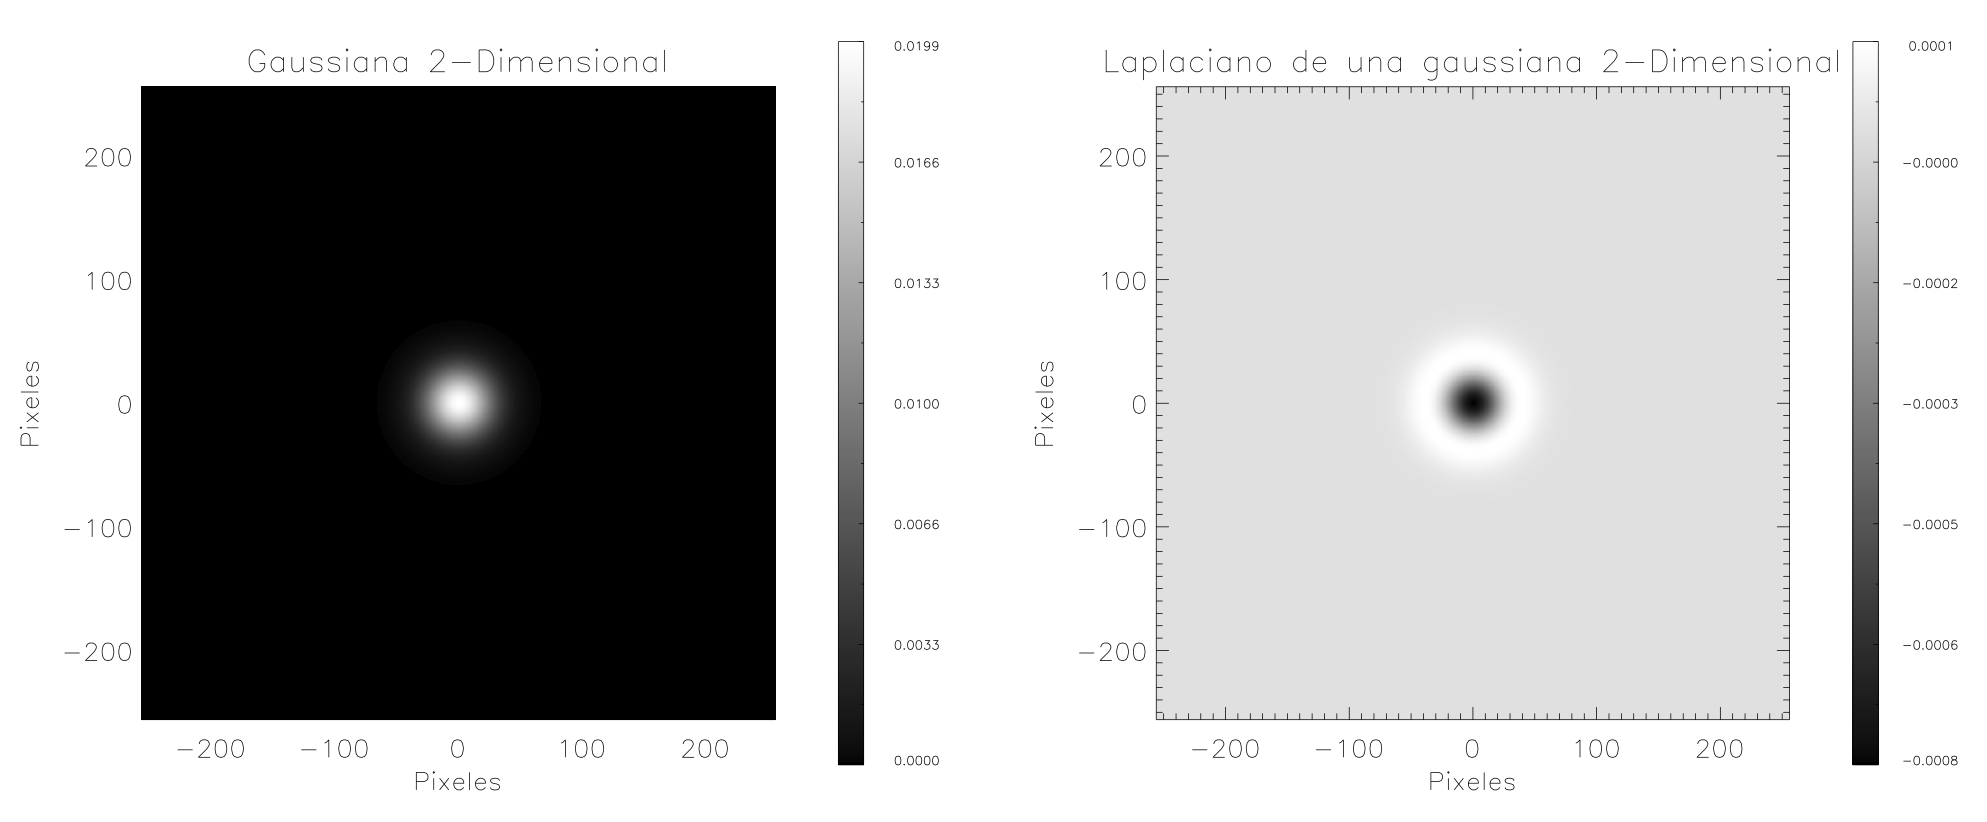
\includegraphics[width=0.55\textwidth]{gauss_lap_teo.png}
}
\caption{{\it Izquierda:} Se\~nal gaussiana bi-dimensional que sigue la expresi\'on dada por la ecuaci\'on  (\ref{eq:gauss}) con un $\sigma=0.8$. {\it Derecha}: Laplaciano de la gaussiana construida siguiendo la forma funcional dada en (\ref{eq:lapgauss}). {\it Arriba:} Visualizaci\'on en 3D. {\it Abajo:} Visualizaci\'on en 2D con escala de grises.}
\label{fig:gauss}
\end{center}
\end{wrapfigure}


\noindent implementado el m\'etodo PASCAL calculando un laplaciano de 5 puntos \citep{detal2006,Lindsey2008,mo2008a,mo2008b,mo2008d,martinez-oliveros2009,matthews2011,zharkov2011}. En este trabajo tomamos los c\'odigos que contienen el m\'etodo PASCAL trabajados por {\it Charles Lindsey} y los modificamos de tal manera que el ajuste del laplaciano se hiciera mediante el algoritmo de 9 puntos con el fin de aplicarlo sobre un evento s\'ismicamente activo, que se conociera muy bien, y poder compararlo con el m\'etodo que usa 5 puntos en aras de encontrar alguna diferencia, el cual es el objetivo de este cap\'itulo. Para poder comparar estos dos algoritmos, lo primero que se debe hacer es aplicarlos sobre una se\~nal conocida y examinar la precisi\'on asociada a cada uno. La primera prueba que se desarrolla es la aplicaci\'on de estos algoritmos sobre una se\~nal {\it gaussiana}, cuya expresi\'on en dos dimensiones es

\begin{align}\label{eq:gauss}
G(x,y)=\frac{1}{\sqrt{2\pi\sigma^2}}\exp\left[-\frac{x^2+y^2}{2\sigma^2}\right],
\end{align} 

\noindent y de la cual es posible conocer te\'oricamente su laplaciano

\begin{align}\label{eq:lapgauss}
\nabla^2G(x,y)=-\frac{1}{\pi\sigma^2}\left(1-\frac{x^2+y^2}{2\sigma^2}\right)\exp\left(-\frac{x^2+y^2}{2\sigma^2}\right).
\end{align}

\begin{SCfigure}
%\begin{center}
\subfloat[]{
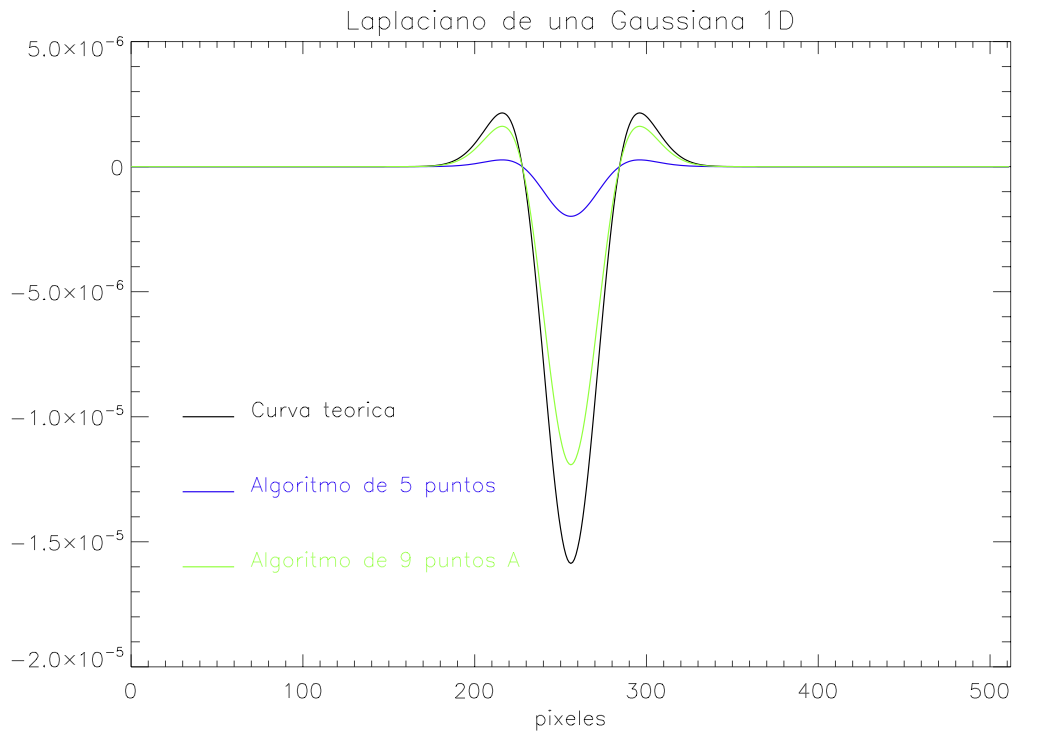
\includegraphics[width=0.35\textwidth]{Laplacian_1D.png}
}
\subfloat[]{
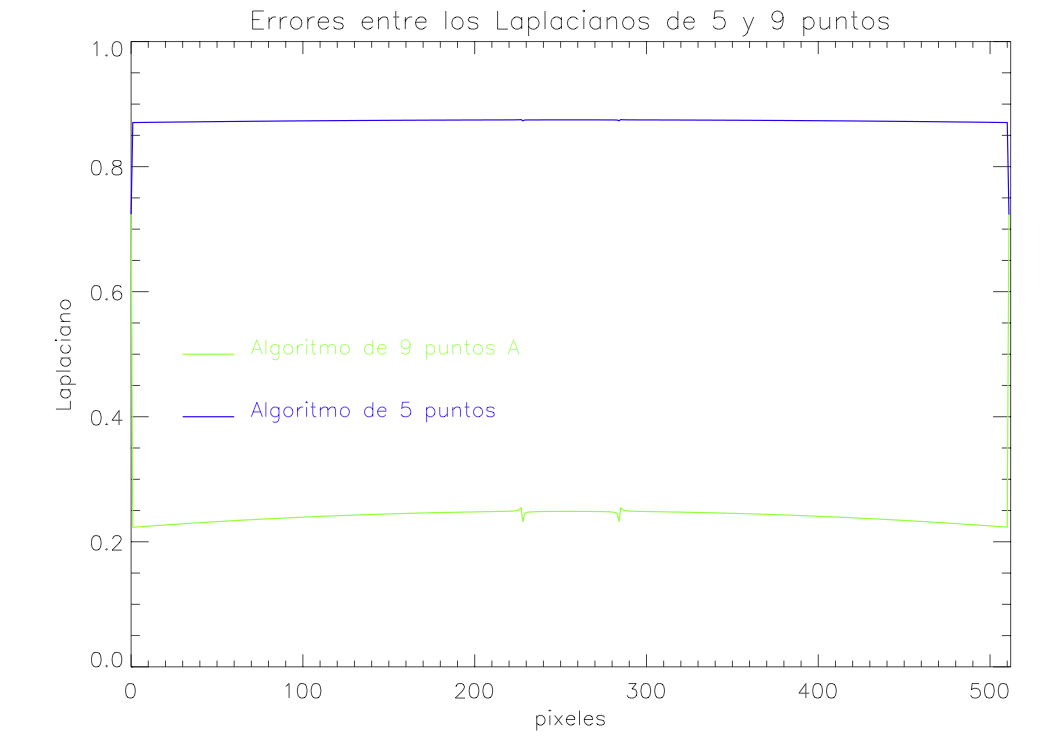
\includegraphics[width=0.35\textwidth]{Laplacian_1D_errores.png}
}
\caption{(a) Comparaci\'on del c\'alculo num\'erico del laplaciano de la se\~nal gaussiana de la figura \ref{fig:gauss} usando los dos algoritmos, el de cinco (curva azul) y el de nueve (curva verde) puntos, y su comparaci\'on con su curva te\'orica (curva negra). (b) Errores de cada uno de los dos m\'etodos con respecto al valor te\'orico.}
\label{fig:perfiles}
%\end{center}
\end{SCfigure}



\noindent En la figura \ref{fig:gauss} se presenta una visualizaci\'on en 3D (arriba) tanto de la se\~nal gaussiana como la de su laplaciano, de acuerdo con las ecuaciones (\ref{eq:gauss}) y (\ref{eq:lapgauss}) respectivamente, con proyecciones planas correspondientes a la variaci\'on de intensidad versus la distancia al centro de la gaussiana, y en la parte inferior de la figura  se han representado las visualizaciones respectivas en un plano de imagen. Para poder hacer una primera comparaci\'on entre los dos m\'etodos usados para calcular num\'ericamente el laplaciano, se hace un corte horizontal que contiene al centro de imagen plana del laplaciano, en nuestro caso al centro de la imagen de la figura \ref{fig:gauss} en la parte baja a la derecha. De esta manera se obtuvieron los perfiles correspondientes al caso te\'o rico como a los dos casos calculados con base en los laplacianos de cinco y de nueve puntos. En la figura \ref{fig:perfiles} la l\'inea negra da cuenta de la curva te\'orica calculada para el laplaciano de una se\~nal gaussiana bidimensional, mientras que las l\'ineas azul y verde representan el c\'alculo num\'erico desarrollado sobre la gaussiana que se muestra en la parte baja de la figura \ref{fig:perfiles} haciendo uso de los m\'etodos de cinco y nueve puntos respectivamente. Claramente, el ajuste con nueve puntos se acerca mucho mejor a la curva te\'orica de lo que lo hace el algoritmo con cinco puntos, como era de esperarse. En la parte (b) de la figura \ref{fig:perfiles} se muestran, adem\'as, los errores porcentuales punto a punto de cada uno de los dos m\'etodos; en dicha gr\'afica se puede apreciar la mejor precisi\'on del m\'etodo de nueve puntos. Ahora bien, una funci\'on gaussiana bidimensional es homog\'enea e isotr\'opica con respecto a su punto central, pero, ?`qu\'e pasar\'ia si ahora aplicamos estos dos mismos m\'etodos de c\'alculo num\'erico sobre una funci\'on que no tenga este par de caracter\'isticas? Para dar respuesta a esta pregunta, se plantea un tratamiento previo a la se\~nal gaussiana que se dividir\'a en dos pasos. El primero consta en amplificar la funci\'on gaussiana a lo largo del eje $x$ en un factor 2 y a comprimirla a lo largo del eje $y$ en un factor $1/2$, y como segundo paso, se calcula nuevamente su laplaciano, tanto te\'orica como num\'ericamente. El resultado es algo como lo que se muestra en la figura \ref{fig:gaussaplastada}. En esta figura se muestra la funci\'on gaussiana achatada (a), su respectivo laplaciano te\'orico (b), el laplaciano num\'erico calculado mediante el algor\'itmo de cinco puntos (c), y el laplaciano num\'erico calculado mediante el algor\'itmo de nueve puntos (d). All\'i se evidencia un diferencia notoria entre el laplaciano te\'orico y los laplacianos num\'ericos, hacia los extremos de la funci\'on a lo largo del eje horizontal.


\begin{figure}[ht!]
\begin{center}
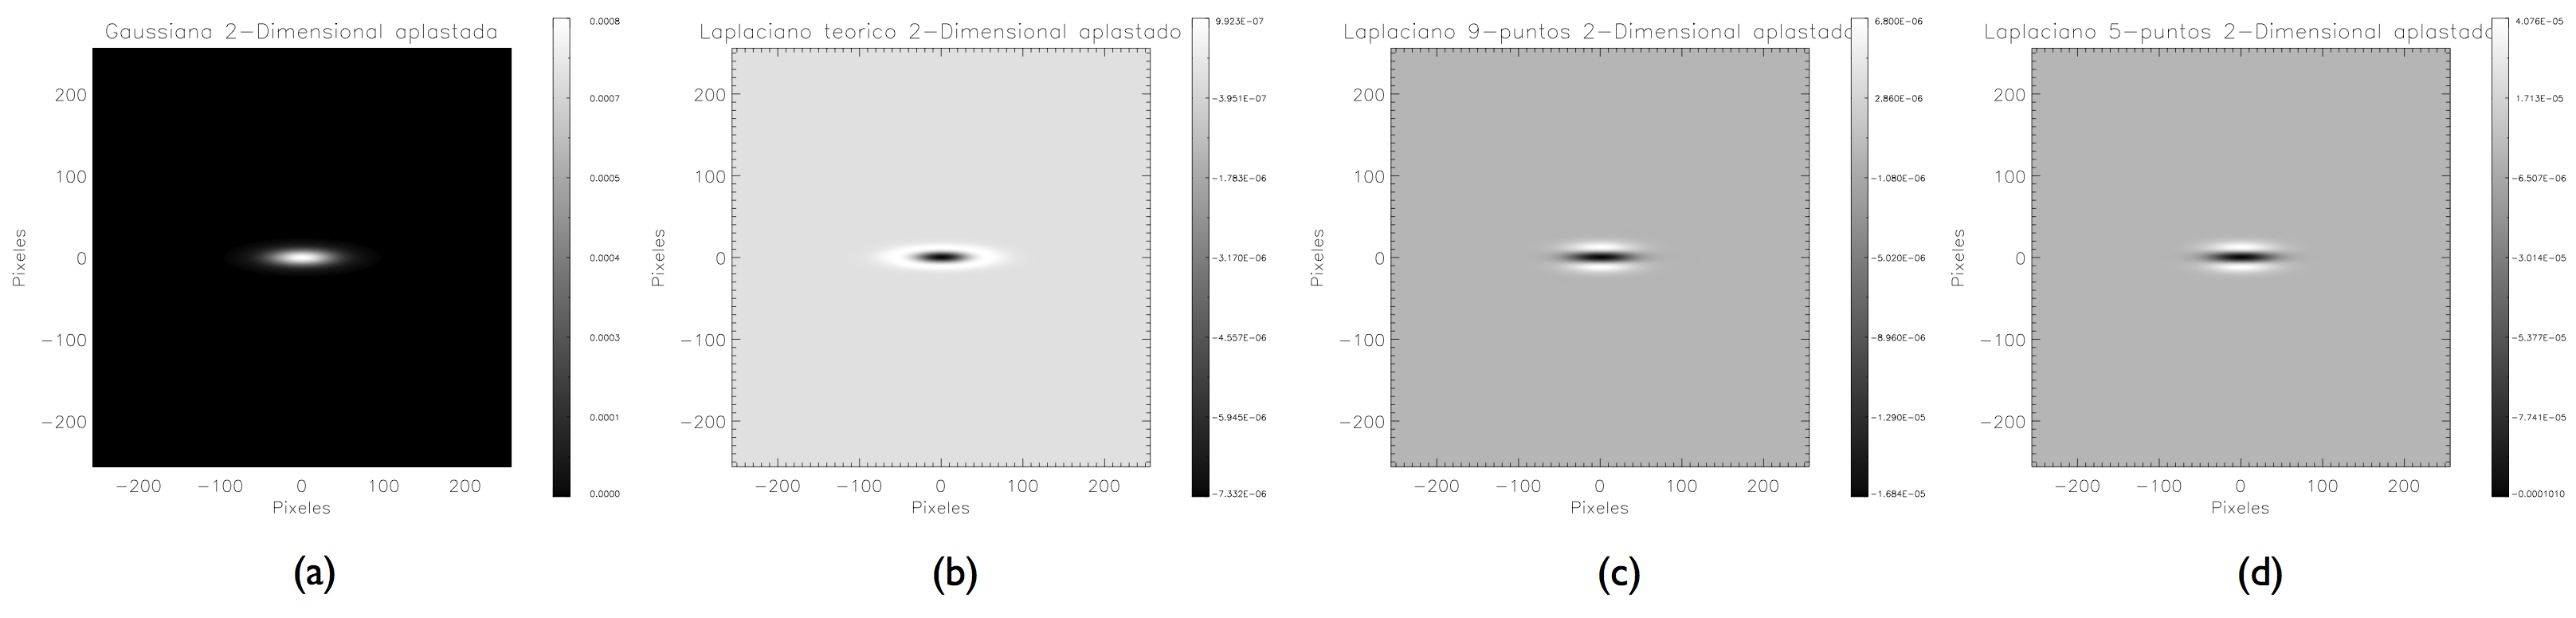
\includegraphics[width=1.0\textwidth]{aplastada.png}
\caption{{\it (a)} Funci\'on gaussiana bidimensional achatada a lo largo del eje vertical y alargada a lo largo del eje horizontal. {\it (b)} Laplaciano te\'orico de la funci\'on gaussiana de la izquierda calculada mediante la implementaci\'on adecuada de la ecuaci\'on (\ref{eq:lapgauss}). {\it (c)} Laplaciano num\'erico calculado mediante la implementaci\'on del algoritmo de cinco puntos.  {\it (d)} Laplaciano num\'erico calculado mediante la implementaci\'on del algoritmo de nueve puntos.}
\label{fig:gaussaplastada}
\end{center}
\end{figure}


Dicha discrepancia es debida a que los algoritmos que se est\'an usando para el c\'alculo num\'erico del laplaciano son definidos para ser trabajados sobre se\~nales (funciones) {\it homog\'eneas}, y claramente la funci\'on gaussiana achatada de la figura \ref{fig:gaussaplastada}(a) no lo es. Dado este escenario, se ve la necesidad de modificar de alguna manera los algoritmos que calculan el laplaciano de manera que se consideren en ellos las formas inhomog\'eneas de las se\~nales bajo estudio. En esta direcci\'on se propone asignar pesos diferentes a los p\'ixeles vecinos de cada p\'ixel sobre el que se lleva a cabo el c\'alculo num\'erico de manera que se contrarresten los efectos de la geometra\'ia no homog\'enea de la funci\'on.\\


\begin{figure}
\begin{center}
\subfloat[]{
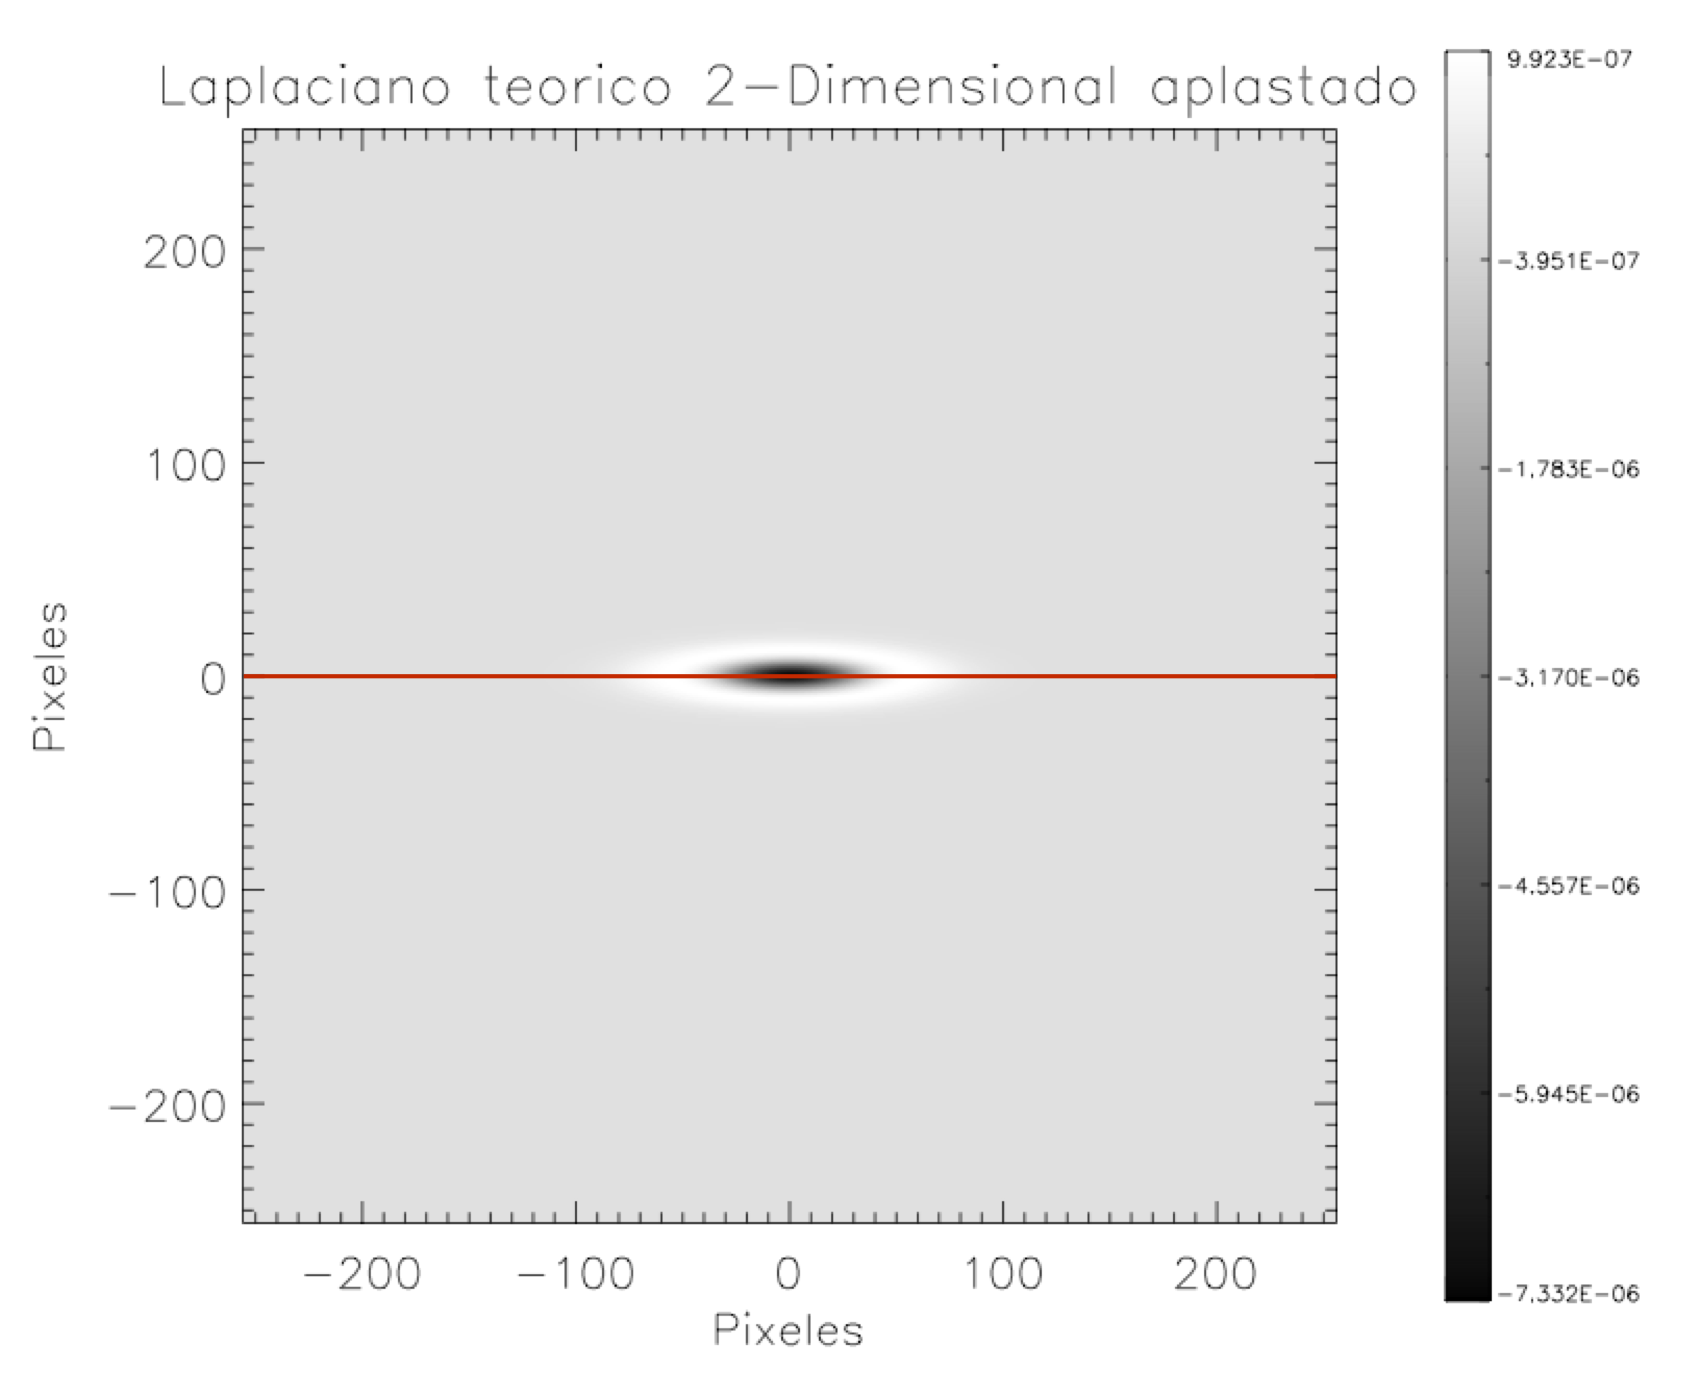
\includegraphics[width=0.3\textwidth]{lapt_aplastada.png}
}
\subfloat[]{
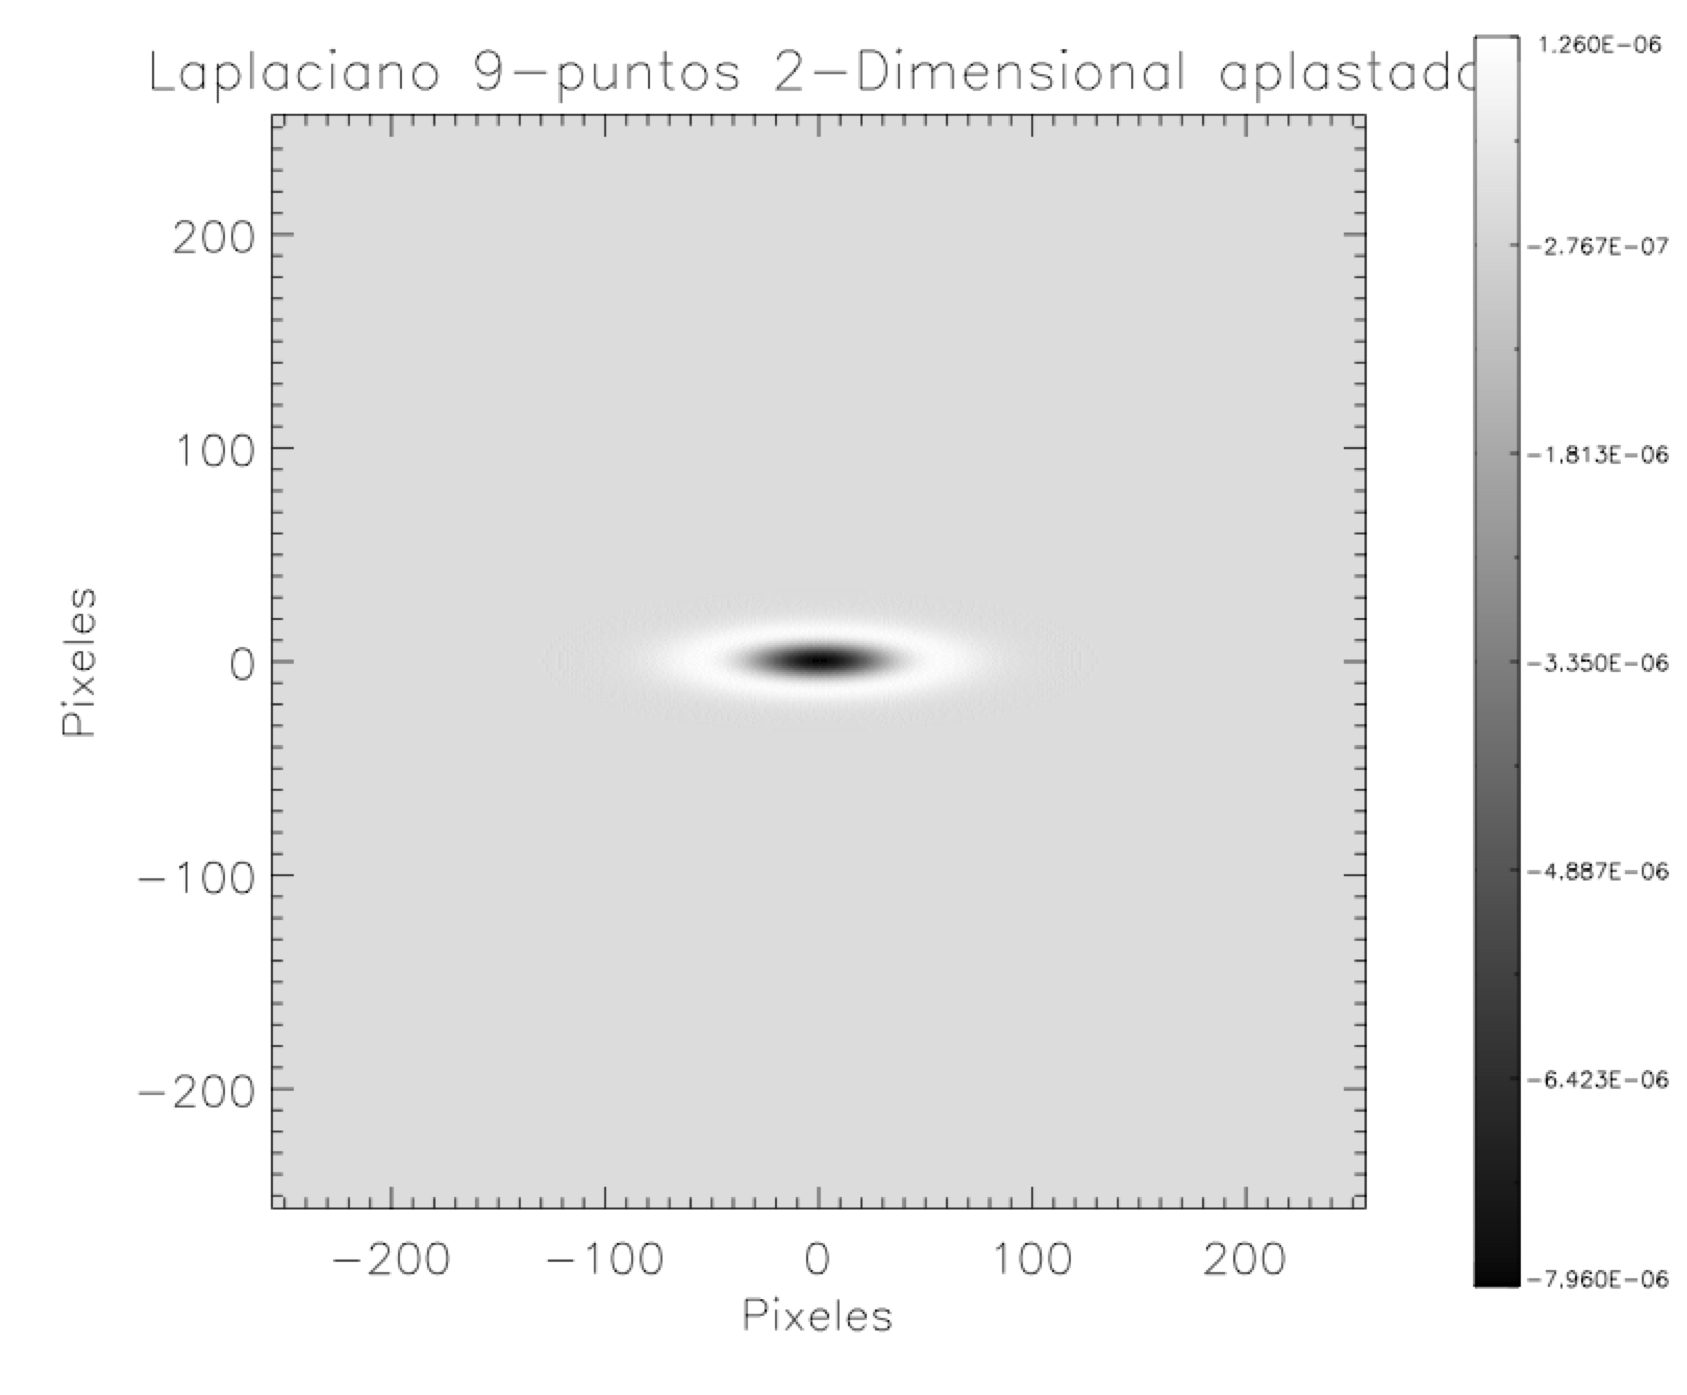
\includegraphics[width=0.3\textwidth]{lap9j_aplastada.png}
}
\subfloat[]{
\includegraphics[width=0.3\textwidth]{Lap_mod_Teo.png}
}
\caption{{\it (a)} Laplaciano te\'orico de la gaussiana achatada de la figura \ref{fig:gaussaplastada}. La l\'inea roja indica la regi\'on escogida para hacer los perfiles que se muestran en (c). {\it (b)} Laplaciano de nueve puntos con pesos asignados por la ecuaci\'on \ref{eq:lapmod} con $\alpha=0.5$, $\beta=2.0$ y $\gamma=0.0$. {\it (c)} Perfiles de comprarci\'on de los dos laplacianos. la curva negra es el perfil te\'orico y la roja es el perfil obtenido mediante el algoritmo de 9 puntos con pesos en sus primeros vecinos. Se error obtiene un error del $15\%$, en promedio, entre las dos curvas.}
\label{fig:lapmod}
\end{center}
\end{figure}


\noindent As\'i, el nuevo algoritmo se expresar\'ia mediante 

\begin{align}\label{eq:lapmod}
\nabla^2I(x_i,y_j)&=f(x_i,y_j),\\\nonumber
f(x_i,y_j)&=\alpha[I(x_i,y_j+1)+I(x_i,y_j-1)-2I(x_i,y_j)]\\\nonumber
&+\beta[I(x_i+1,y_j)+I(x_i-1,y_j)-2I(x_i,y_j)]\\\nonumber
&+\frac{\gamma}{4}[I(x_i+1,y_j+1)-I(x_i-1,y_j+1)-I(x_i+1,y_j-1)+I(x_i-1,y_j-1)],\label{eq:lapmod}
\end{align}


\noindent en donde $\alpha$, $\beta$, $\gamma$ son los par\'ametros escalares que dan peso a los primeros y segundos vecinos, del p\'ixel sobre el que se realiza el c\'alculo, a lo largo del eje horizontal, del eje vertical y de los ejes diagonales respectivamente. Para su implementaci\'on, por ejemplo, en el caso considerado en la figura \ref{fig:gaussaplastada}, un buen ajuste se consigue al definir $\alpha=0.5$, $\beta=2.0$ y $\gamma=0.0$. Un perfil horizontal sobre dicho ajuste con su respectiva comparaci\'on con el valor te\'orico de \'este se muestran en la figura \ref{fig:lapmod}. De esta figura se evidencia una clara mejor\'ia en el ajuste del m\'etodo n\'umerico con la curva te\'orica y se corrobora al hacer el c\'alculo de su error porcentual de un $15\%$ en promedio.\\

Siguiendo con la prueba de funcionalidad del c\'alculo num\'erico del laplaciano, se plantea ahora rotar la funci\'on con respecto al origen coordenado en una cantidad de $45^\circ$ y $315^\circ$ como se muestra en la figura \ref{fig:gausssquezee}. Observe que la l\'inea roja trazada en la figura \ref{fig:lapmod} es la misma que aparece en la figura \ref{fig:gausssquezee}. Este m\'etodo da origen a una se\~nal que emular\'ia a la funci\'on gaussiana vista de perfil, es decir, algo as\'i como si esta proviniera de un lugar en la superficie solar m\'as cerca hacia el limbo del disco solar observado desde la tierra. Esto se hace justamente en busca de evaluar la precisi\'on de cada m\'etodo sobre se\~nales que no necesariamente se hayan presentado en el centro del disco del Sol, pues como es bien sabido una fulguraci\'on solar puede presentarse en cualquier regi\'on sobre el discosolar. Para la se\~nal de la parte superior de la figura \ref{fig:gausssquezee}, la cual ha sido rotada un \'angulo de $45^\circ$, tomamos los par\'ametros $\alpha=1.0$, $\beta=1.0$ y $\gamma=1.6$ en aras de contrarrestar el efecto de la proyecci\'on y de darle un mayor peso a la direcci\'on diagonal inclinada un \'angulo de $45^\circ$ en el sentido antihorario, obteniendo as\'i el laplaciano num\'erico bidimensional que se muestra en la parte izquierda de la figura \ref{fig:lapjc45}. As\'i mismo, sobre la l\'inea roja horizontal, de esta misma figura, se traz\'o el perfil de la gaussiana para verificar de manera unidimensional la calidad de su ajuste. Este perfil se muestra al lado derecho de la figura \ref{fig:lapjc45}. El error promedio de este laplaciano num\'erico no homog\'eneo es del $5\%$ con respecto a la curva te\'orica calculada. Dada la antisimetr\'ia del conjunto de t\'erminos que da cuenta de las contribuciones diagonales en el c\'alculo del laplaciano num\'erico dado por la ecuaci\'on \ref{eq:lapmod}, se espera que para una gaussiana modificada de la misma manera que esta \'ultima que trabajamos pero con una rotaci\'on neta de $315^\circ$ en sentido antihorario los coeficientes que asignan peso a cada p\'ixel de la vecindad inmediata est\'en dados por $\alpha=1.0$, $\beta=1.0$ y $\gamma=-1.6$. Al desarrollar este procedimiento se encuentra algo como lo que se muestra en la figura \ref{fig:lapjc315} y de igual forma se asocia un error promedio del $5\%$.\\


\begin{SCfigure}
\centering
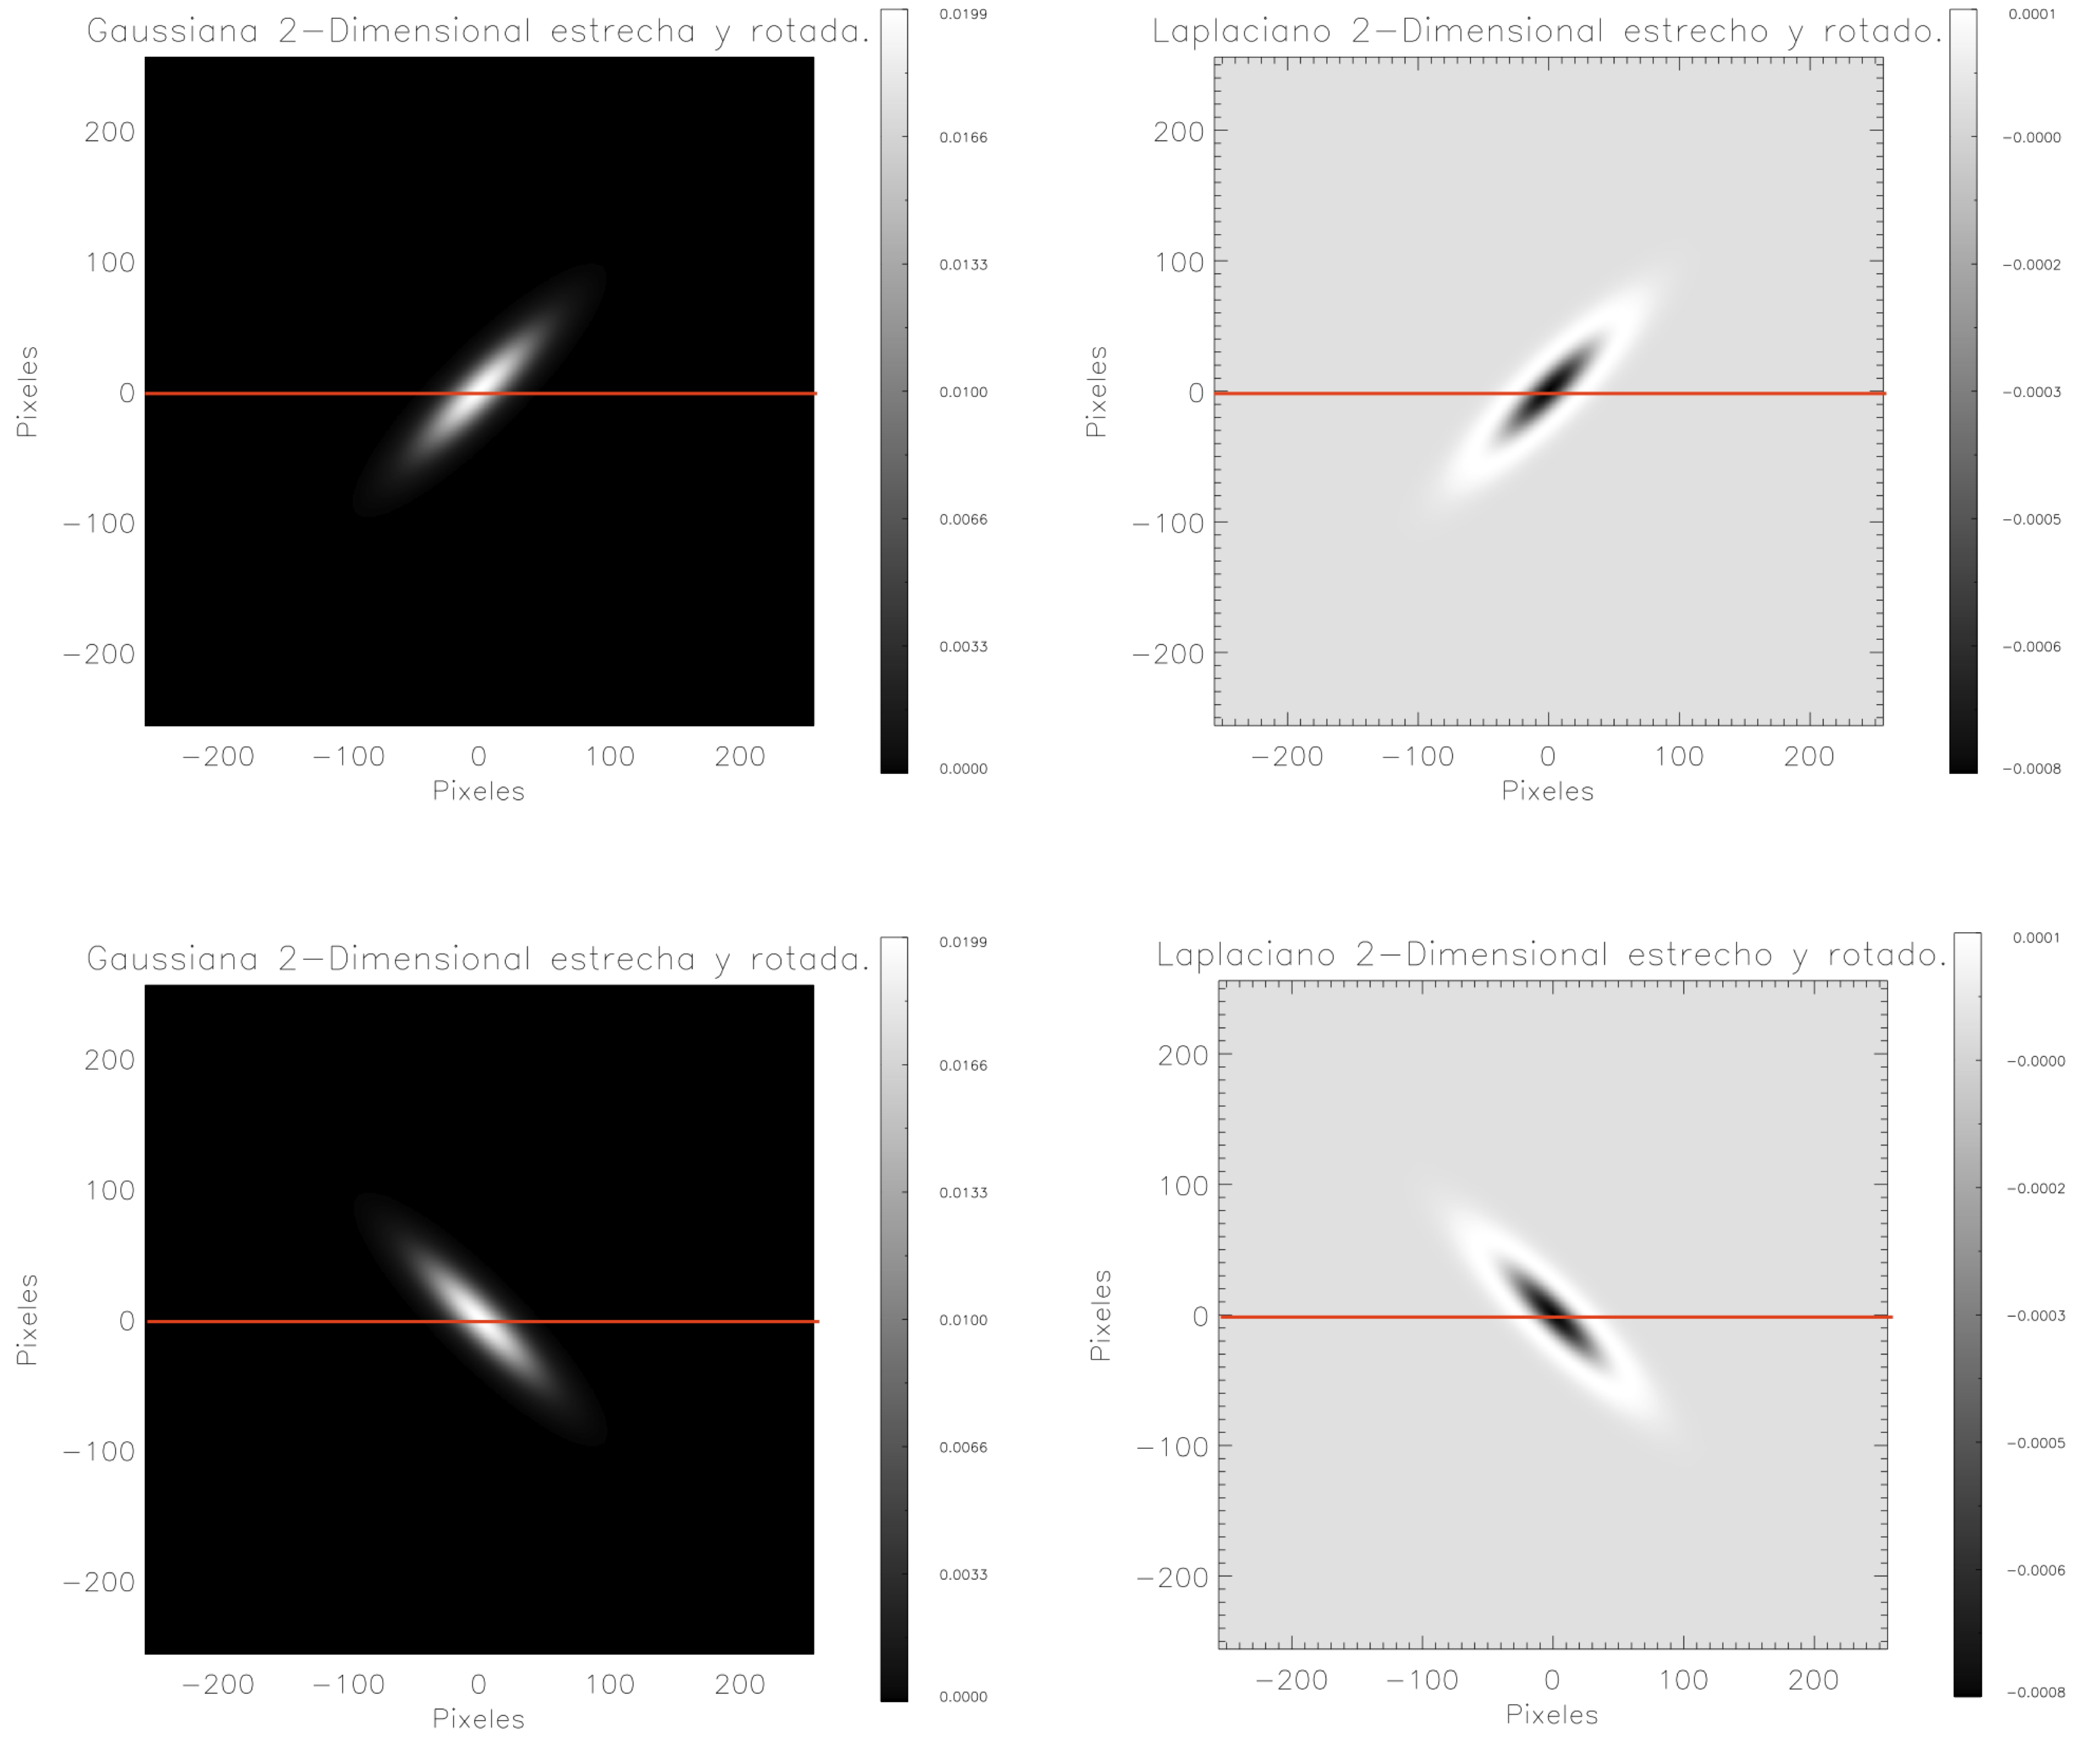
\includegraphics[width=0.7\textwidth]{gausss.png}
\caption{{\it Izquierda:} Se\~nal gaussiana bidimensional que ha sido estirada y luego rotada. {\it Derecha:} Laplaciano te\'orico de cada una de las se\~nales gaussianas a la izquierda. {\it Arriba:} se\~nal gaussiana rotada $45^\circ$. {\it Abajo:} Se\~nal gaussiana rotada $315^\circ$. Las l\'ineas rojas indican el eje de corte escogido para trazar el perfil de cada una de las se\~nales para ser comparados con los algoritmos de c\'alculo num\'erico.}
\label{fig:gausssquezee}
%\end{center}
\end{SCfigure}


\begin{figure}
\begin{center}
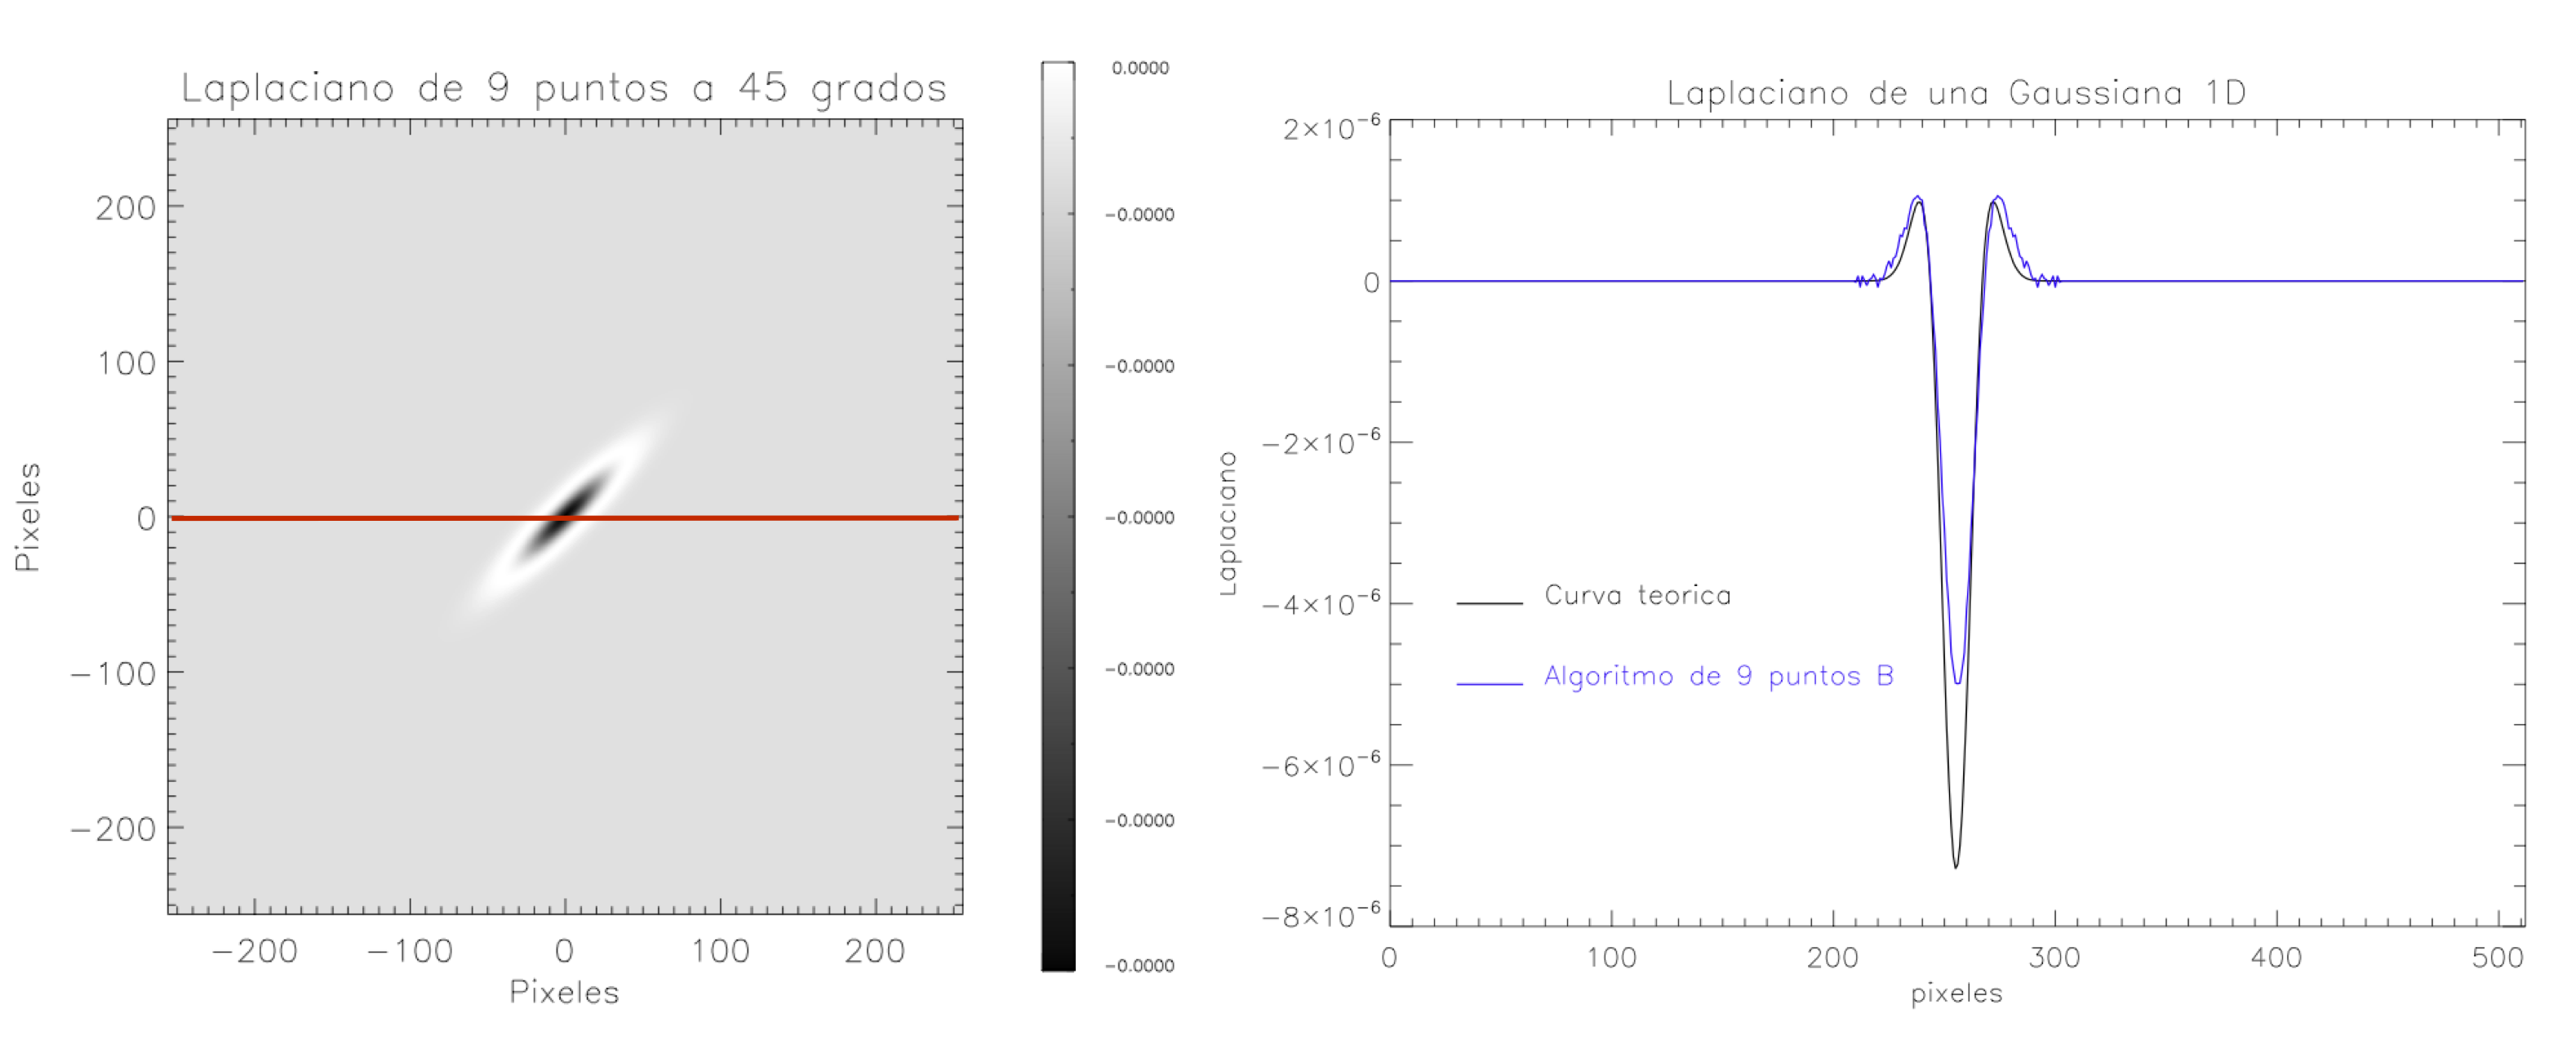
\includegraphics[width=0.95\textwidth]{lap_sq_45.png}
\caption{{\it Derecha}: Laplaciano dos dimensional de una gaussiana achatada y rotada $45^\circ$ calculado con el algoritmo dado por la ecuaci\'on \ref{eq:lapmod} con $\alpha=1.0$, $\beta=1.0$, $\gamma=1.6$. La l\'inea roja indica el lugar por donde se traz\'o el perfil unidimensional que se muestra en la gr\'afica de la {\it izquierda}. El error promedio encontrado entre el ajuste num\'erico y la curva te\'orica es del $5\%$.}
\label{fig:lapjc45}
\end{center}
\end{figure}


\begin{figure}
\begin{center}
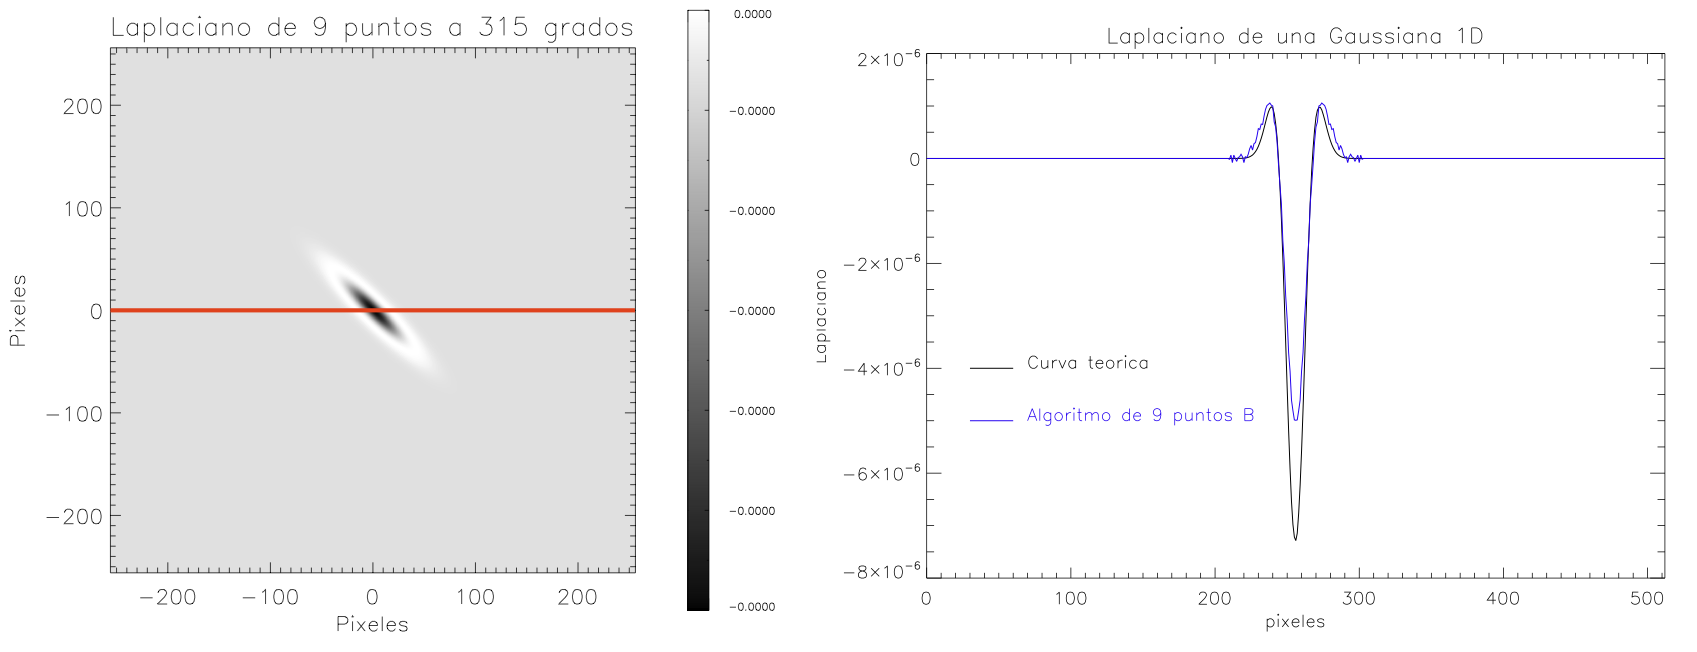
\includegraphics[width=0.95\textwidth]{lap_sq_315.png}
\caption{{\it Derecha}: Laplaciano dos dimensional de una gaussiana achatada y rotada $315^\circ$ calculado con el algoritmo dado por la ecuaci\'on \ref{eq:lapmod} con $\alpha=1.0$, $\beta=1.0$ y $\gamma=-1.6$. La l\'inea roja indica el lugar por donde se traz\'o el perfil unidimensional que se muestra en la gr\'afica de la {\it izquierda}. El error promedio encontrado entre el ajuste num\'erico y la curva te\'orica es del $5\%$.}
\label{fig:lapjc315}
\end{center}
\end{figure}

Ahora bien, con este conjunto de pruebas que se han hecho sobre la forma en la que se debe modificar el algoritmo que calcula el laplaciano de nueve puntos sobre una se\~nal que no es homog\'enea ni isotr\'opica, y al comprobar su correcto funcionamiento, lo que nos ata\~ne ahora es encontrar la forma en la que estos coeficientes $\alpha$, $\beta$ y $\gamma$, que dan peso a los p\'ixeles de la vecindad dependiendo de la geometr\'ia de la se\~nal, deben ser definidos para que este procedimiento de c\'alculo num\'erico pueda ser aplicado correctamente sobre una se\~nal f\'isica real proveniente de alg\'un lugar sobre la superficie solar. En este orden de ideas debemos relacionar el valor de estos tres coeficientes con una proyecci\'on postel que se haga del fotograma tomado del Sol centrado en la regi\'on de inter\'es, la regi\'on activa asociada a la fulguraci\'on que en nuestros casos pudo dar pie a la generaci\'on de un helio-sismo.

\subsection*{Proyecciones heliogr\'afica y postel aplicadas a un fotograma solar}
\addcontentsline{toc}{subsection}{Proyecciones heliogr\'afica y postel aplicadas a un fotograma solar}

La red de telescopios en tierra GONG++ nos ha prove\'ido de fotogramas de muy buena calidad y resoluci\'on desde Julio de 2001. As\'i, se ha convertido en una fuente importante de datos para el desarrollo de an\'alisis basados en las t\'ecnicas propias de la heliosismolog\'ia; nosotros en particular estamos interesados en heliosismolog\'ia local. Para este tipo de an\'alisis es necesario proveerse de unos arreglos de datos en tres dimensiones conocidos en la comunidad de cient\'ificos solares como {\it cubo de datos}. Esto es, dado el deseo de caracterizar temporalmente una regi\'on determinada que se encuentra sobre la superficie solar es necesario hacer un seguimiento de esta al transcurrir el tiempo. De esta manera este conjunto de datos espacio-temporal se puede definir en la pr\'actica mediante el uso de un arreglo (o cubo de datos) de $N_x\times N_y\times N_t$ elementos, en donde $N_x$ y $N_y$ representan el n\'umero de elementos en cada una de las dimensiones espaciales, y $N_t$ es el n\'umero de pasos temporales. Claramente, la calidad del an\'alisis heliosismol\'ogico que se desarrolle va a depender fuertemente de la calidad de la forma en la que se construya dicho cubo de datos, y de aqu\'i la importancia de este procedimiento.\\

En un marco de referencia geoc\'entrico el Sol no es para nada un objeto inmutable y/o en reposo. El Sol tiene un movimiento anual de traslaci\'on a lo largo de la ecl\'iptica, un movimiento de rotaci\'on con respecto a su eje polar y unos movimientos m\'as finos dados por la precesi\'on y nutaci\'on de su eje polar. El conjunto completo de estos movimientos debe ser corregido por un seguimiento excelso de la regi\'on de inter\'es en aras de construir un cubo de datos adecuado. Para esto \cite{lb2000} han propuesto un par de transformaciones, una transformaci\'on heliogr\'afica acompa\~nada de una proyecci\'on {\it Postel}, en el marco de la definici\'on de su m\'etodo propio de {\it holograf\'ia ac\'ustica}.\\

La primera transformaci\'on que se lleva a cabo es una transformaci\'on de coordenadas heliogr\'aficas a coordenadas cartesianas helioc\'entricas. Para esto es necesario conocer la longitud de {\it Carrington}, $L_{ij}(t_k)$, y la latitud heliogr\'afica\footnote{Estas coordenadas son conocidas como las {\it coordenadas de Carrington}. Estas coordenadas son una variaci\'on del sistema coordenado heliogr\'afico que rota a una velocidad angular igual a la tasa de rotaci\'on media del Sol tal y como fue definido originalmente por Carrington (1863). El periodo sideral del sistema de Carrington es de 25.38 d\'ias, lo cual implica un periodo sin\'odico de 27.2753 d\'ias. \cite[]{thompson2005}}, $B_{ij}(t_k)$, para todo elemento con coordenadas $i,j$ en todo $t_k$, en donde $i\in N_x$, $j\in N_y$ y $t_k\in N_t$. Esto es posible, si en particular se conocen las coordenadas de Carrington de un determinado punto sobre el disco solar. Para este fin, cada uno de los observatorios de la red GONG++ registra en los {\it encabezados} de los archivos fits las coordenadas de {\it Carrington} instant\'aneas del punto {\it sub-tierra}, que es aquel punto que se genera en la intersecci\'on de la la superficie solar con la l\'inea recta que une al centro de la tierra con el centro del Sol (instant\'aneos) cada vez que se toma un fotograma. Esto, salvo un peque\~no error por paralaje, coincide con el punto ubicado en el centro del disco solar definido sobre las im\'agenes que se toman. De esta manera, para poder hacer una descripci\'on completa es necesario definir un tiempo de referencia para el punto central: $M_0=M_{00}(t_0)$ dado por $B_0=B_{00}(t_0)$ y $L_0=L_{00}(t_0)$. Adem\'as, se necesita definir un conjunto de im\'agenes ordenadas temporalmente seg\'un el momento en el que fueron tomadas y separadas por el tiempo caracter\'istico dado por la cadencia de los instrumentos que se est\'an usando para la medida (en el caso de GONG la cadencia es de un minuto). As\'i, $t_k=t_0+k\Delta t$ donde $\Delta t$ es la cadencia caracter\'istica de los instrumentos y $k=-N_t/2,...,-1,0,1,...,N_t/2$.\\

\begin{figure}
\centering
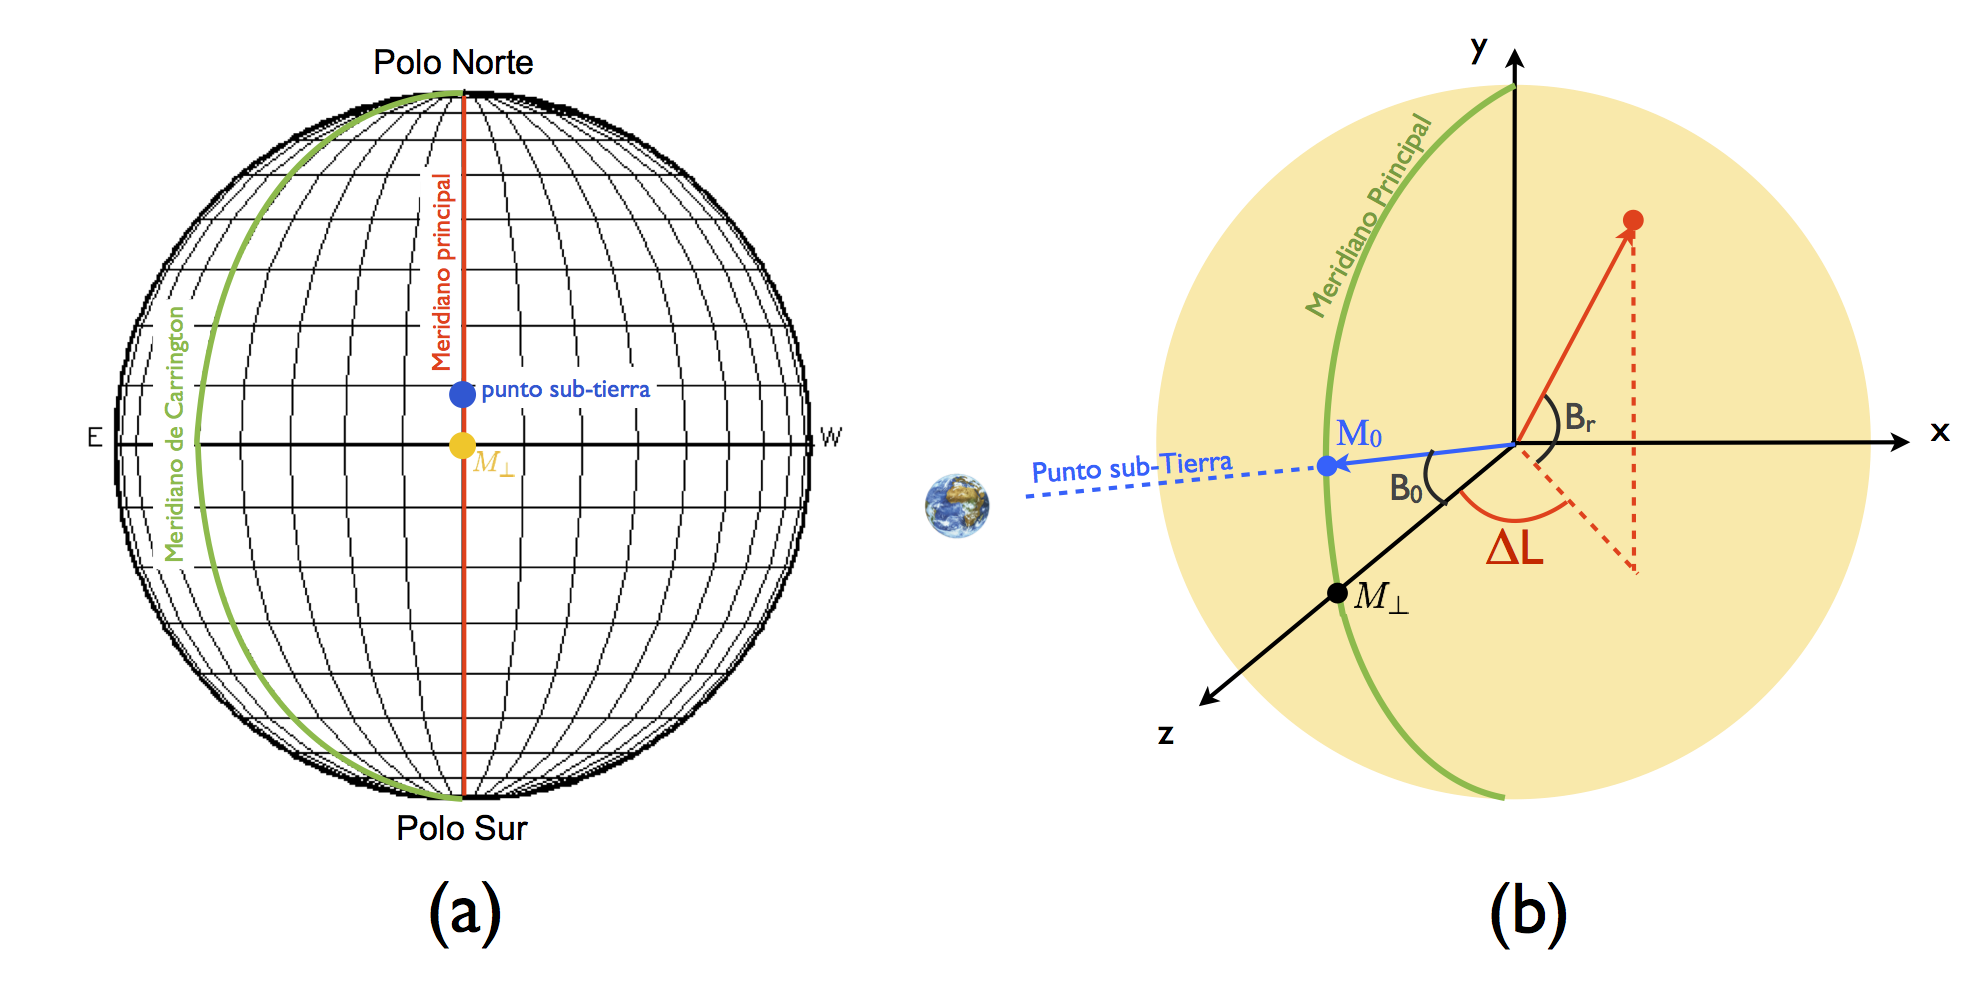
\includegraphics[width=0.65\textwidth]{carrington1.png}
\caption{{\bf (a)}. Representaci\'on gr\'afica del {\it punto sub-tierra} (en azul), el meridiano principal (en rojo), el meridiano de Carrington (en verde) y el punto de intersecci\'on entre el meridiano principal y el c\'irculo m\'aximo perpendicular a \'el en un marco de referencia heliogr\'afico cuya grilla se indica en negro. {\bf (b)} Sistema coordenado cartesiano en tres dimensiones, con origen en el centro del solar, en donde se definen el punto {\it sub-tierra} (punto azul sobre la superficie), el meridiano principal (semic\'irculo verde), y el punto $M_\bot$ en la intersecci\'on entre el meridiano principal y el c\'irculo m\'aximo helioc\'entrico perpendicular al eje $y$. Un punto arbitrario sobre la superficie solar se puede ubicar mediante la asignaci\'on de valores $\Delta L$ y $B_r$.}
\label{fig:carrington}
\end{figure}

Adem\'as, denotamos como $R$ al sistema de coordenadas heliogr\'aficas de {\it Carrington},  sobre \'el $M_0$ es el punto {\it sub-tierra}, $M$ representa al meridiano principal (en ingl\'es {\it prime meridian}), el cual se define como el semic\'irculo m\'aximo que une a los dos polos heliogr\'aficos y que contiene a $M_0$. El punto $M_{\bot}$ se define como la intersecci\'on entre el meridiano principal y el c\'irculo m\'aximo trazado sobre la heliosfera perpendicular a \'el ({\it ecuador solar}), tal como se esquematiza en la figura \ref{fig:carrington}(a).  Podemos introducir un sistema cartesiano de coordenadas con origen en el centro del Sol, cuyo eje $y$ est\'a orientado a lo largo del eje polar, y el eje $z$ est\'a orientado en la direcci\'on radial hacia el punto $M_\bot$.  Una transformaci\'on entre las coordenadas heliogr\'aficas esf\'ericas, por el momento con radio unitario, y las coordenadas cartesianas definidas arriba, viene dada por el siguiente conjunto de ecuaciones:

\begin{align}
\begin{pmatrix}
x\\
y\\
z
\end{pmatrix}
=
\begin{pmatrix}
\cos B_{xy}\sin L_{xy}\\
\sin B_{xy}\\
\cos B_{xy}\cos L_{xy}
\end{pmatrix},
\end{align}

\noindent esto para un determinado tiempo $t_k$. Ahora bien, la necesidad de manipular las im\'agenes del Sol de forma tal que queden perfectamente alineadas una detr\'as de la otra a la hora de construir el cubo de datos nos enfrenta a la necesidad de corregir las im\'agenes por el conjunto completo de movimientos que afectan a la visual del disco solar minuto a minuto en el registro de los fotogramas, adem\'as de hacer una proyecci\'on {\it Postel} correcta sobre la regi\'on de inter\'es. Supongamos que nuestra regi\'on de inter\'es est\'a en una posici\'on arbitraria sobre el disco solar, como se representa mediante el punto rojo en la figura \ref{fig:carrington}(b). A dicho punto le corresponden las coordenadas heliogr\'aficas $L_r$ (longitud de {\it Carrington}) y  $B_r$ (latitud de {\it Carrington}). As\'i, en el sistema coordenado R de la figura \ref{fig:carrington}(b) las coordenadas helioc\'entricas de dicha regi\'on van a estar dadas por

\begin{align}
\begin{pmatrix}
x_r\\
y_r\\
z_r
\end{pmatrix}
=
\begin{pmatrix}
\cos B_r\sin \Delta L\\
\sin B_r\\
\cos B_r\cos \Delta L
\end{pmatrix},
\end{align}

\noindent en donde $\Delta L$ es la diferencia entre las longitudes de {\it Carrington} del punto $r$ y el punto {\it sub-tierra} $M_0$. Ahora bien, un sistema coordenado $R'$ con origen en el centro del Sol y cuyo eje $z'$ se dirige a lo largo del punto {\it sub-tierra} se puede definir a trav\'es de las coordenadas en $R$ mediante una rotaci\'on coordenada sencilla a lo largo del eje $x$, como se esquematiza en la figura \ref{fig:rotacion}. De esta manera, las coordenadas de nuestra regi\'on de inter\'es representadas en el sistema coordenado $R'$ estar\'an dadas por:

\begin{align}
\begin{pmatrix}
x'_r\\
y'_r\\
z'_r
\end{pmatrix}
=
\begin{pmatrix}
1 & 0 & 0 \\
0 & \cos B_0 & -\sin B_0\\
0 & \sin B_0 & \cos B_0 
\end{pmatrix}
\begin{pmatrix}
x_r\\
y_r\\
z_r
\end{pmatrix}.
\end{align}

\begin{wrapfigure}[20]{r}{0.45\textwidth}
\begin{center}
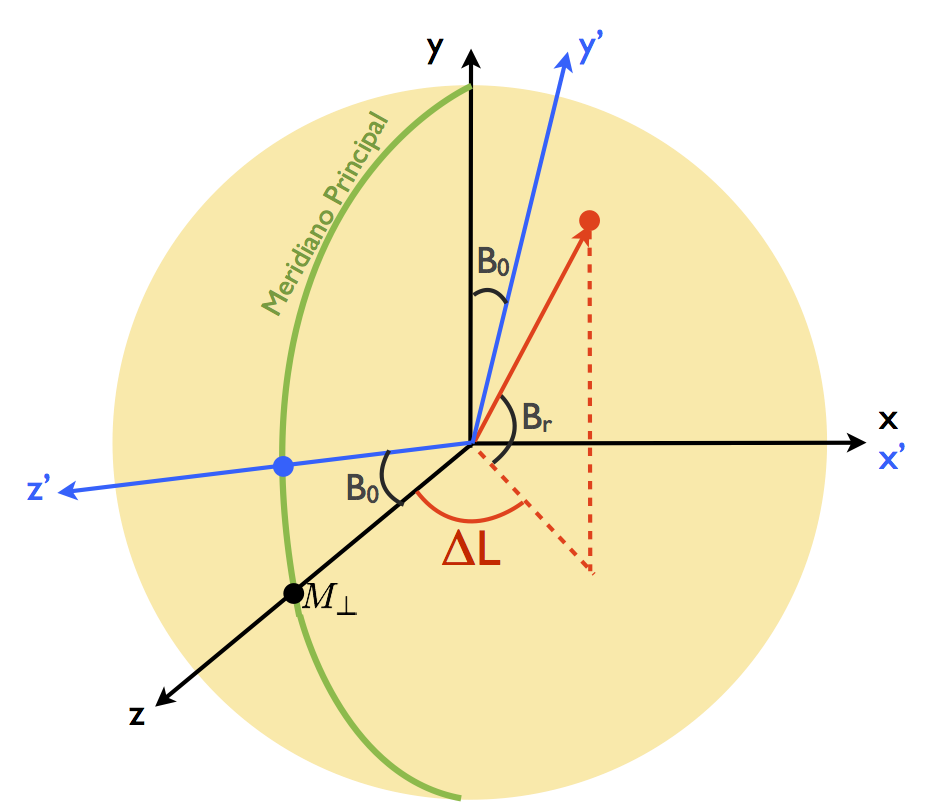
\includegraphics[width=0.42\textwidth]{rotacion.png}
\caption{Definici\'on de un sistema coordenado $R'$, de coordenadas $x',y',z',$ en azul, que est\'a rotado un \'angulo $B_0$ con respecto al eje $x$ del sistema $R$ (en negro).}
\label{fig:rotacion}
\end{center}
\end{wrapfigure}

Como la regi\'on para analizar se puede ubicar en cualquier posici\'on sobre la superficie solar, se sigue inmediatamente que este conjunto de ecuaci\'on es extrapolable a cualquier punto arbitrario, obteniendo de esta manera las ecuaciones expuestas en (\ref{eq:transform}).

\begin{align}\label{eq:coordenadas}
\cos\theta'\sin\varphi'&=\cos B_r\sin\Delta L\\\nonumber
\sin\theta'&=-\cos B_r\sin B_0\cos\Delta L+\sin B_r\cos B_0\\\nonumber
\cos\theta'\cos\varphi'&=\cos B_0\cos B_r\cos \Delta L+\sin B_0\sin B_r.
\end{align}

Con esto se logra alinear apropiadamente todos los fotogramas en la muestra temporal $N_t$ de manera que ya es posible construir el cubo de datos sin problemas, ya que existe un movimiento relativo Sol-observador debido tanto a la rotaci\'on del Sol como al movimiento del observador mismo en su descripci\'on helio\'entrica, de modo tal que para cada instante de tiempo se asume que se conocen $L_0$ y $B_0$ de las efem\'erides f\'isicas del Sol. En seguida, la tarea consiste en llevar a cabo la proyecci\'on {\it Postel} de este \'ultimo sistema coordenado cartesiano $R'$ al plano imagen del fotograma, y para esto hacemos uso de las expresiones mostradas en (\ref{eq:postel}).\\

Siguiendo lo visto en el cap\'itulo anterior, es necesario considerar la posici\'on de la regi\'on de inter\'es sobre el disco solar para poder asignar los pesos correctos al algoritmo de c\'alculo del laplaciano de nueve puntos (\ref{eq:lapmod}) y de esta manera implementar el m\'etodo de limpieza PASCAL sobre las im\'agenes de ciencia sin ning\'un inconveniente. En esta direcci\'on, lo que se hace es definir cuatro par\'ametros $a_{11},a_{12},a_{21},a_{22}$ que forman parte de la matriz $\mathbf{A}$ definida de la siguiente manera:

\begin{align}
\mathbf{A}=
\begin{pmatrix}
a_{11} & a_{12}\\
a_{21} & a_{22}
\end{pmatrix}
=
\begin{pmatrix}
[\sin B_0\sin B_r \cos\Delta L + \cos B_0\cos B_r] & \sin B_r \sin\Delta L\\
-\sin B_0 \sin\Delta L & \cos \Delta L
\end{pmatrix}\frac{1}{z'_r},
\end{align}

\noindent donde 

\begin{align}
\alpha&\equiv a_{11}^2+a_{12}^2\\\nonumber
\beta&\equiv a_{11}^2+a_{12}^2\\\nonumber
\gamma&\equiv 2 (\,a_{11}a_{21}+a_{22}a_{12}).
\end{align}


N\'otese que si la regi\'on de inter\'es se ubica justamente en el centro del disco solar de los fotogramas, es decir, se satisface $\Delta L=0$ y $B_r=B_0$, se cumple que $\alpha=1$, $\beta=1$ y $\gamma=0$; lo que era de esperarse pues en este caso la regi\'on de inter\'es ser\'ia localmente homog\'enea e isotr\'opica y por lo tanto la expresi\'on (\ref{eq:lapmod}) se reduce al algoritmo dado por (\ref{eq:lap5}) con $h=1$.

\section*{Implementaci\'on del m\'etodo PASCAL sobre una muestra de fulguraciones energ\'eticas}
\addcontentsline{toc}{section}{Implementaci\'on del m\'etodo PASCAL sobre una muestra de fulguraciones energ\'eticas}


Como se mencion\'o anteriormente, en la secci\'on de~\nameref{sec:sismicidad}, se han reportado eventos de fulguraciones solares s\'ismicamente activas con una correlaci\'on local fuerte de una emisi\'on grande y repentina en luz blanca. \cite{detal2006} reportaron por primera vez una coincidencia fuerte entre la ubicaci\'on de la fuente s\'ismica, determinada a partir de los mapas de egresi\'on construidos a trav\'es de la t\'ecnica de holograf\'ia ac\'ustica, y tres n\'ucleos compactos y bien definidos de emisi\'on en luz blanca para un evento que tuvo lugar el 9 de Septiembre de 2001 a las 20:40 TU. Esto \'ultimo soporta la hip\'otesis de que el calentamiento repentino de la fotosfera es un proceso que podr\'ia estar ligado a la generaci\'on repentina de una onda mec\'anica transitoria que podr\'ia, a su vez, estar relacionada con la aparici\'on de una fuente s\'ismica. Algunos autores han propuesto diferentes mecanismos posibles que tratan de dar una explicaci\'on plausible de los procesos f\'isicos que podr\'ian estar involucrados detr\'as del calentamiento repentino de la fotosfera. Por ejemplo, \cite{dl2005} y \cite{zharkova2008} argumentan que el calentamiento de la fotosfera podr\'ia ocurrir por la interacci\'on directa de protones energ\'eticos  y/o electrones {\it altamente} energ\'eticos con el ambiente del plasma local. Particularmente  \cite{zharkova2008} le da una prelaci\'on importante a los protones, por encima de los electrones, por su poder alto de penetraci\'on en la materia. Sin embargo, algunos otros trabajos \cite[]{kosovichev2007a} sugieren que los protones acelerados no constituyen una fuente adecuada para dar pie a una respuesta hidrodin\'amica en el plasma de la atm\'osfera solar, y por lo tanto dif\'icilmente podr\'ian estar relacionados con la generaci\'on de la fuente s\'ismica asociada a un {\it sunquake} y, a su vez, con el aumento en la emisi\'on de luz blanca altamente localizada tanto espacial como temporalmente. Aunque en estos trabajos se sugiere el {\it back-warming} como posible mecanismo responsable de la emisi\'on en luz blanca que aqu\'i se menciona, otros trabajos ponen en duda cualquier clase de correlaci\'on entre estos dos fen\'omenos \citep[]{isobe2007,potts2010}.\\

De cualquier manera, y sea como sea que el aumento en la emisi\'on de luz blanca asociada a fulguraciones solares sea producida, trabajos relativamente recientes \citep[]{detal2006,pedram2012} han mostrado una correlaci\'on aparente entre la emisi\'on en luz blanca y algunos heliosismos observados durante la fase impulsiva (definida en la banda de los rayos-X suaves) de aquellas fulguraciones alta o moderadamente energ\'eticas que tuvieron lugar a lo largo del ciclo solar 23. Esto hace que las fulguraciones a las que se les asocia una emisi\'on fuerte en luz blanca se conviertan en buenos candidatos a la hora de buscar eventos fulgurantes s\'ismicamente activos, adem\'as de poder utilizarlos adecuadamente en el estudio y entendimiento de la generaci\'on y din\'amica de los {\it sunquakes}.\\

Por otro lado, en el trabajo extensivo de buscar y caracterizar fulguraciones solares s\'ismicamente activas, todo un conjunto de trabajos que usan las t\'ecnicas de holograf\'ia ac\'ustica y de diagrama de tiempo-distancia \cite[]{besliu2005,detal2006,kz2006c,kosovichev2007a,alvarado2012}, han encontrado un buen n\'umero de eventos en los que las se\~nales s\'ismicas est\'an altamente correlacionadas, tanto temporal como espacialmente, con la aparici\'on de fuentes compactas de emisi\'on en rayos-X duros. Estas observaciones han dado pie a otras tantas explicaciones que tratan de dar cuenta de los mecanismos f\'isicos propios de la fenomenolog\'ia que se esconde detr\'as de la generaci\'on de los heliosismos. Por ejemplo, \cite{zharkova2008} sugiere que la emisi\'on en rayos-X duros de todos estos eventos est\'an relacionados de alguna manera con la precipitaci\'on hacia capas m\'as internas del Sol de part\'iculas altamente energ\'eticas y su posterior dep\'osito de energ\'ia en estas regiones.\\

Dada la importancia de las fulguraciones con una emisi\'on alta en luz blanca, as\'i como en rayos-X duros en el estudio de los {\it sunquakes}, se decidi\'o implementar los c\'odigos de limpieza del m\'etodo PASCAL sobre una muestra de fulguraciones que en lo posible tuvieran estas dos caracter\'isticas, as\'i como la de estar localizadas cerca del centro del disco solar en donde los Dopplergramas ofrecen una confiabilidad mayor. Adem\'as, decidimos centrar nuestra atenci\'on sobre los eventos ocurridos en lo que llevamos del ciclo solar 24, pues es el periodo temporal que en estos momentos nos ofrece el mayor n\'umero de fulguraciones sin explorar. En esta direcci\'on, se empez\'o por hacer un filtrado de la lista completa de fulguraciones observadas por el instrumento espacial RHESSI. Para ello, acudimos a la lista publicada permanentemente en \hyperref[http://hesperia.gsfc.nasa.gov/rhessi2/home/data-access/rhessi-data/flare-list/]{http://hesperia.gsfc.nasa.gov/rhessi2/home/data-access/rhessi-data/flare-list/}, y tomamos aquellas fulguraciones que hayan registrado una emisi\'on discernible por los detectores en energ\'ias por encima de los 50 keV y que hayan tenido lugar en el periodo comprendido entre el 1 de Enero de 2010 y el 30 de Julio de 2012\footnote{El 30 de Julio de 2012 fue el \'ultimo d\'ia en que se revis\'o la lista de fulguraciones de RHESSi en el marco de esta tesis. Claramente como para esta fecha a\'un no estamos en el m\'aximo de actividad solar de este ciclo, se espera que en fechas posteriores se encuentren m\'as fulguraciones con las caracter\'isticas que buscamos.}. De esta manera obtuvimos un total de 51 eventos, de los cuales s\'olo 28 ten\'ian una ubicaci\'on cercana al centro del disco solar adecuadas para desarrollar un an\'alisis heliosismol\'ogico. Es de se\~nalar adem\'as que de estas \'ultimas 28 fulguraciones 4 registraron una emisi\'on discernible por RHESSI en la banda de los 100 keV a los 300 keV. Para escoger  estas 28 fulguraciones se procedi\'o a calcular su distancia al centro del disco solar haciendo uso de las coordenadas helioc\'entricas \cite[]{thompson2005} de la fulguraci\'on dadas por RHESSI. Los 28 eventos que se muestran en el cuadro \ref{tb:fulguraciones} son tales que su distancia al centro del disco solar es menor que 600 segundos de arco.\\

El paso siguiente fue buscar los respectivos fotogramas en intensidad de cada uno de los  eventos de la tabla \ref{tb:fulguraciones}. Esto se hizo a trav\'es del servidor oficial de la red GONG++, \hyperref[http://gong2.nso.edu/archive/patch.pl?menutype=s]{http://gong2.nso.edu/archive/patch.pl?menutype=s}. No todos los eventos fueron observados por los telescopios de la red, algunas veces  por malas condiciones atmosf\'ericas, as\'i como por alg\'un posible problema en la calibraci\'on de los datos. De aqu\'i que solamente los {\bf 10} eventos que se se\~nalan en el cuadro \ref{tb:fulguraciones} son de los que se tienen datos de estos instrumentos. As\'i mismo, se aprovecha el cuadro \ref{tb:fulguraciones} para se\~nalar aquellos eventos para los cuales el {\it Helioseismic and Magnetic Imager} a bordo del {\it Solar Dynamic Observatory}, y del que hablaremos m\'as adelante en detalle, registr\'o datos. 

\begin{table}
\caption{Lista de fulguraciones altamente energ\'eticas registradas por RHESSI en rayos-X duros, con emisiones por encima de los 50 keV, durante el periodo comprendido entre el 1 de Enero de 2010 y el 30 de Julio de 2012. La primera columna numera cronol\'ogicamente los eventos, la segunda columna muestra la fecha en la que ocurrieron; las tercera, cuarta y quinta columnas muestran el comienzo, el pico y el final de la emisi\'on en una banda entre los y los keV para cada uno de los eventos respectivamente. La sexta y la s\'eptima columnas muestran la ubicaci\'on de la fulguraci\'on. La novena columna da el n\'umero de la regi\'on activa, y en las casillas d\'ecima y und\'ecima se\~nalamos si el evento fue registrado por la red GONG y/o por HMI/SDO respectivamente.}
\begin{center}
\begin{tabular}{l r r r r r r r r r r}
\toprule[0.8mm]
\# &    Fecha        & Comienzo &      Pico      &     Final     &   X   &   Y    &   AR   & GONG & HMI/SDO\\
\bottomrule[0.8mm]
1   & 2010-02-08 &  07:31:16   &  07:41:26  & 07:53:32  &  034 & 474 & 1045  & &  \\
2   & 2010-02-12 &  11:21:28   &  11:26:14  & 11:36:24  & -169 & 515 & 1046  & \checkmark  & \checkmark  \\
3   & 2010-10-16 &  19:08:48   &  19:12:18  & 19:34:40  & 394 & -397 & 1112  & \checkmark  & \checkmark  \\
4   & 2011-02-14 &  04:41:12   &  04:44:10  & 05:25:04  & 031 & -223 & 1158  & \checkmark  & \checkmark  \\
5   & 2011-02-15 &  01:43:44   &  01:55:30  & 02:27:32  & 205 & -222 & 1158  & \checkmark  & \checkmark  \\
6* & 2011-03-07 &  19:40:12   &  20:04:54  & 20:07:48  & 624 & 556 & 1164  & \checkmark  & \checkmark  \\
7   & 2011-03-09 &  23:10:28   &  23:22:18  & 23:38:08  & 191 &  272 &  ---  & \checkmark  & \checkmark  \\
8   & 2011-07-30 &  02:05:32   &  02:09:10  & 02:29:24  & -526 & 170 & 1261  & \checkmark  & \checkmark  \\
9   & 2011-08-03 &  04:29:24   &  04:31:58  & 04:43:28  & -155 & 166 &  ---  & \checkmark  & \checkmark  \\
10 & 2011-08-04 &  03:42:28   &  03:46:58  & 03:47:40  &  537 & 201 & ---   & \checkmark  & \checkmark  \\
11*& 2011-09-06 &  22:08:00   &  22:19:46  & 22:25:04  &  284 & 133 & 1283   & \checkmark  & \checkmark  \\
12 & 2011-09-08 &  15:33:00   &  15:43:50  & 16:02:00  &  610 & 147 & 1283  & \checkmark  & \checkmark  \\
13 & 2011-09-26 &  05:05:16   &  05:07:58  & 05:14:40  &  -519 & 116 & 1302  & \checkmark  & \checkmark  \\
14 & 2011-12-25 &  20:24:12   & 20:27:54  & 20:35:52  &  369 & -334 & 1387  & \checkmark  & \checkmark  \\
15 & 2011-12-27 &  04:07:32   & 04:18:38  & 04:38:36  &  -494 & -250 & 1386  & \checkmark  & \checkmark  \\
16*& 2012-03-04 &  11:06:52   & 11:07:30  & 11:10:44  &  617 & -666 & ---  & \checkmark  & \checkmark  \\ 
17 & 2012-03-09 &  04:24:36  & 04:27:54  & 04:37:08  &  0 & 389 & 1429  & \checkmark  & \checkmark  \\
18 & 2012-05-09 &  12:29:48  & 12:30:30  & 12:43:00  &  -488 & 242 & 1476  & \checkmark  & \checkmark  \\
19 & 2012-05-09 &  14:10:04  & 14:10:46  & 14:27:32  &  -353 & 162 & 1476  & \checkmark  & \checkmark  \\
20 & 2012-05-10 &  04:13:08  & 04:17:42  & 04:29:36  &  -364 & 259 & 1476  & \checkmark  & \checkmark  \\
21*& 2012-06-03 &  17:49:24  & 17:54:46  & 18:01:20  &  -570 & 275 & 1493  & \checkmark  & \checkmark  \\
22 & 2012-07-02 &  19:47:04  & 20:05:18  & 20:11:56  &  -16 & -325 & 1514  & \checkmark  & \checkmark  \\
23 & 2012-07-04 &  09:49:04  & 09:54:26  & 10:14:32  &  289 & -343 & 1515  & \checkmark  & \checkmark  \\
24 & 2012-07-04 &  16:33:00  & 16:37:06  & 16:46:48  &  484 & -184 & 1513  & \checkmark  & \checkmark  \\
25 & 2012-07-05 &  03:26:20  & 03:35:50  & 03:55:16  &  417 & -338 & 1515  & \checkmark  & \checkmark  \\
26 & 2012-07-05 &  11:39:52  & 11:44:14  & 11:53:08  &  495 & -332 & 1515  & \checkmark  & \checkmark  \\
27 & 2012-07-06 &  01:27:16  & 01:39:38  & 02:13:04  &  585 & -322 & 1515  & \checkmark  & \checkmark  \\
28 & 2012-07-12 &  16:49:52  & 16:50:54  & 17:28:08  &  14 & -308 & 1520  & \checkmark  & \checkmark  \\
%\cmidrule(l){2-4}
%Juan&40& 60 & 100 \$\\
%\midrule
%Pedro&70& 30 & 100 \$\\
%\cmidrule[0.5mm](l){4-4}
%& & & 200 \$ \\
\bottomrule[0.8mm]
\end{tabular}
\end{center}
\label{tb:fulguraciones}
\end{table}



%%%%%%%%%%%%%%%%%%%%%%%%%%%%%%%%%%%%%%%%%%%

%\begin{wrapfigure}[20]{r}{0.65\textwidth}
%\begin{center}
%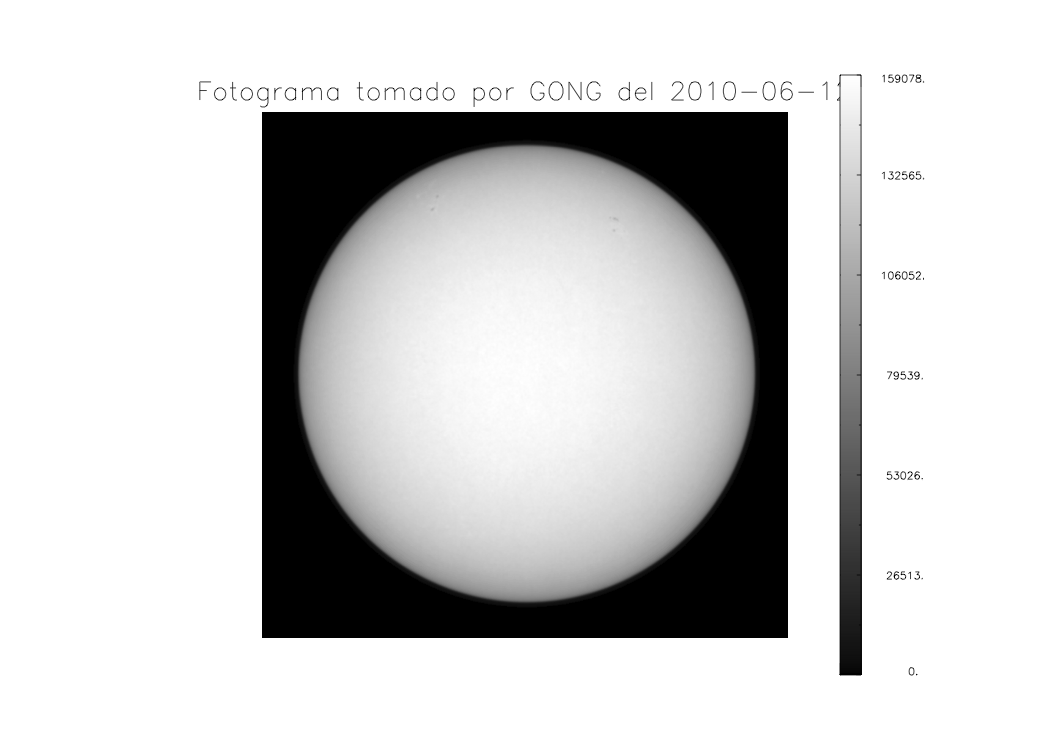
\includegraphics[width=0.65\textwidth]{gong.png}
%\caption{Fotograma en luz blanca del Sol el 12 de Junio de 2012 por el Observatorio Mauna Loa HI USA de la red de telescopios terrestres GONG++.}
%\label{fig:gong}
%\end{center}
%\end{wrapfigure}


%Hablar de que todos los trabajos han considerado m�todos de 5 puntos, y que nosotros lo comparamos con el de 9 y describir lo que encontramos... depu�s hablar de Sergey y sus im�genes mostrar unas de nuestras im�genes si las hay.








%\input{gong_pascal.tex}
%\input{sergey.tex}
%\input{pascal_transientes.tex}
%\input{mecanismos_sismos.tex}
\newpage
\pagestyle{fancy}
\chapter*{Aceleraci\'on estoc\'astica de part\'iculas en una fulguraci\'on solar}
\addcontentsline{toc}{chapter}{Aceleraci\'on estoc\'astica de part\'iculas en una fulguraci\'on solar}



\renewcommand{\baselinestretch}{1.0}

\begin{wrapfigure}[29]{r}{0.46\textwidth}
\begin{center}
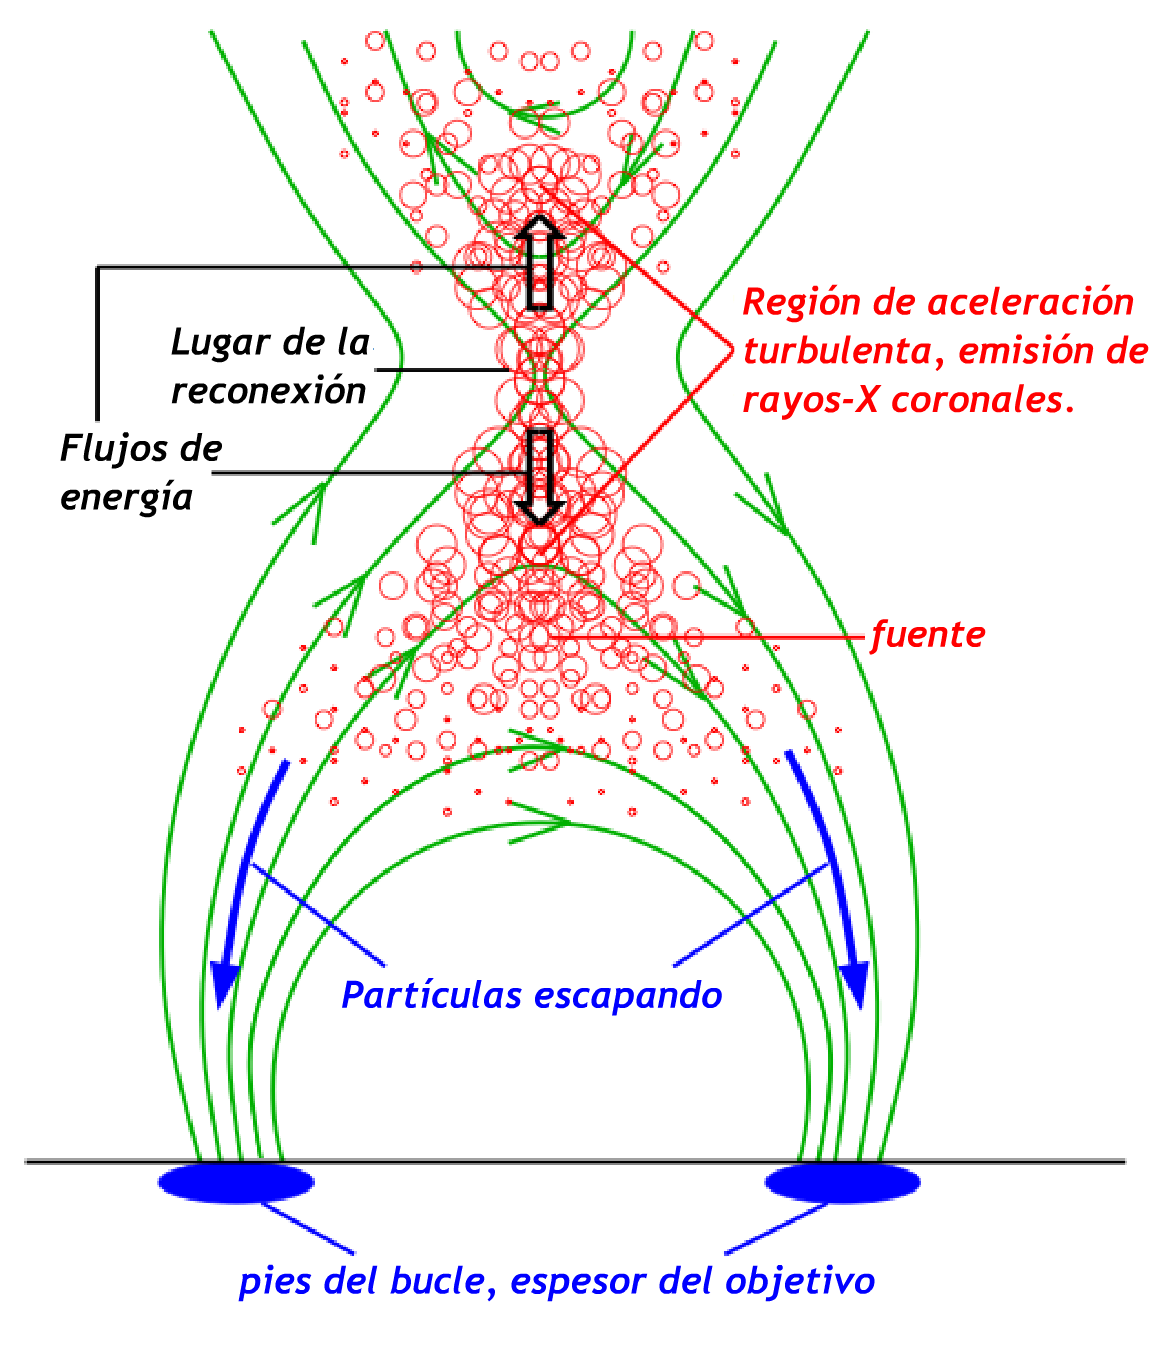
\includegraphics[width=0.39\textwidth]{wei-liu.png}
\caption{Esquema del modelo de aceleraci\'on estoc\'astica propuesto para las fulguraciones solares. Las curvas en verde representan las l\'ineas de campo magn\'etico en una configuraci\'on posible; los c\'irculos en rojo representan la turbulencia o las ondas del plasma que se generan durante el evento de la fulguraci\'on. {\it Tomado y modificado de} \citep[]{liu2008}.}
\label{fig:liu}
\end{center}
\end{wrapfigure}

En el estudio de las fulguraciones solares se trabaja b\'asicamente con tres mecanismos diferentes de aceleraci\'on de part\'iculas: (1) {\bf Aceleraci\'on directa por acci\'on de un campo el\'ectrico}: \citep[]{HOLMAN1985,wood2005} Se plantea que la aceleraci\'on del {\it jet}\footnote{Usamos aqu\'i el t\'ermino en ingl\'es {\it jet} para referirnos a un haz de part\'iculas tipo chorro, para estar m\'as acorde con la nomenclatura internacional al respecto.} de part\'iculas cargadas se lleva a cabo mediante una aplicaci\'on sencilla de una fuerza tipo Coulomb mediante un campo el\'ectrico DC que se genera sobre la zona de reconexi\'on; el problema m\'as grande que sobrelleva este modelo es la dificultad de mantenerlo a gran escala. (2) {\bf Aceleraci\'on de Fermi a primer orden (choque)}: \citep[]{Tsuneta1998} Este mecanismo plantea que la manera en la que se les suministra energ\'ia a las part\'iculas es cuando son embestidas por un frente de una onda de choque producto de un hipot\'etico {\it jet super-magnetos\'onico} proveniente de la regi\'on de reconexi\'on. Adem\'as, este proceso deja ver escalas de tiempo del orden de los 0.3 - 0.6 s que est\'an de acuerdo con las observaciones. Aunque esta din\'amica ofrece una explicaci\'on plausible de la inyecci\'on de las part\'iculas hacia el interior solar, tiene algunos problemas en cuanto a las consecuencias que traer\'ia sobre las part\'iculas que saldr\'ian expelidas hacia el espacio interplanetario. (3) {\bf Aceleraci\'on estoc\'astica o aceleraci\'on de Fermi a segundo orden}: La turbulencia y las ondas de plasma son los eventos m\'as comunes que est\'an presentes cuando se da un evento de fulguraci\'on solar \citep[]{petrosian1994,miller1998}. En el modelo de {\it aceleraci\'on estoc\'astica} el esquema b\'asico de la din\'amica propuesta es como la que se presenta en la figura \ref{fig:liu}. 

Como una consecuencia de la reconexi\'on magn\'etica bien sea mediante la turbulencia a gran escala o bien mediante las ondas de plasma que son generadas cerca del punto-X de reconexi\'on, las part\'iculas son aceleradas, y estas, a su vez, producen una emisi\'on en rayos-X duros que se producen cerca de la cima del bucle de la fulguraci\'on en el llamado {\it thin target}, como producto de una emisi\'on t\'ermica por parte de las part\'iculas  aceleradas. El registro de esta emisi\'on ha sido uno de los mayores logros de la misi\'on {\it Yohkoh}. Las part\'iculas que no son atrapadas en la cima y que logran escapar hacia la parte baja de la atm\'osfera solar, al interactuar con el plasma que rodea los pies del bucle, emiten tambi\'en en rayos-X duros por radiaci\'on {\it Bremsstrahlung} y forman los conocidos {\it thick target} en las vecindades de los {\it footpoints}.\\

Este mecanismo ha sido profundamente estudiado por diversos autores no solamente en el marco del estudio de las fulguraciones solares sino en varias otras ramas de la astrof\'isica que involucran este tipo de procesos como en los agujeros negros, en los {\it Gamma Ray Burts} (GRB), los n\'ucleos activos de galaxias, etc \citep[]{park1996,1996miller,1997park,Liu2004A}.\\


Usualmente cuando en f\'isica se habla de un proceso estoc\'astico se debe hacer referencia a la ecuaci\'on de {\it Boltzmann}. Pues bien, trabajos desarrollados por \cite{F1914} y \cite{P1917} a principios del siglo pasado mostraron todo un desarrollo en cuanto a la teor\'ia existente detr\'as de un proceso de aceleraci\'on estoc\'astica de un ensamble de part\'iculas puntuales con la posibilidad de poder introducir en este formalismo diferentes interacciones entre ellas y fuerzas externas a ellas. Gracias a esto, hoy en d\'ia esta ecuaci\'on se conoce como la ecuaci\'on de {\it Fokker-Planck}, la cual ser\'a el tema de la siguiente secci\'on.


\section*{Ecuaci\'on de Fokker-Planck}
\addcontentsline{toc}{section}{Ecuaci\'on de Fokker-Planck}

La ecuaci\'on de {\it Fokker-Planck} b\'asicamente brinda un formalismo que permite estudiar la din\'amica de un sistema de muchas part\'iculas en el cual los efectos de las colisiones entre ellas cobran una importancia relevante en el planteamiento de su din\'amica.\\

Hacia comienzos del siglo XX, y despu\'es de que Einstein hubiese propuesto su hip\'otesis del movimiento {\it browniano} en uno de sus famosos art\'iculos de 1905\footnote{En 1905 Albert Einstein public\'o su art\'iculo titulado: ``{\it \"{U}ber die von der molekularkinetischen Theorie der W\"arme geforderte Bewegung von in ruhenden Fl\"ussigkeiten suspendierten Teilchen}'' (Sobre la teor\'ia cin\'etica-molecular del calor requerido por el movimiento de part\'iculas suspendidas en l\'iquidos en reposo) en el {\it Annalen der Physik} en que planta las bases del atomismo moderno dando una explicaci\'on razonable del movimiento aleatorio que presentan part\'iculas peque\~nas suspendidas sobre un estanque de agua en reposo.}, se centraron muchos esfuerzos en analizar este ``curioso'' comportamiento de movimiento aleatorio que registraban las part\'iculas subat\'omicas. En busca de esto se desarrollaron una variedad de experimentos en los que por ejemplo se enfriaba Hidr\'ogeno l\'iquido hasta temperaturas muy cercanas al cero absoluto con el fin de observar el movimiento de un conjunto de semillas peque\~nas que se depositaban sobre su superficie. Al mismo tiempo, se trabajaba en desarrollos te\'oricos en aras de establecer un formalismo te\'orico que brindara explicaci\'on a este comportamiento; en este sentido fue {\it A.D. Fokker} quien en 1914 public\'o su trabajo titulado ``{\it Die mittlere Energie rotierender elektrischer Dipole im Strahlungsfeld}'' o  `` Energ\'ia media de rotaci\'on de dipolos el\'ectricos inmersos en un campo de radiaci\'on'', en el cual por primera vez muestra un tratamiento estoc\'astico con el objetivo de ligar este comportamiento aleatorio de naturaleza microsc\'opica con variables observables a nivel macrosc\'opico \citep[]{F1914}. Tres a\~nos m\'as tarde, {\it Planck} recoge y complementa los trabajos de {\it Fokker} y publica un art\'iculo en el que formaliza una ecuaci\'on que trabaja con la din\'amica de las part\'iculas involucradas en el espacio de fases y construye un formalismo regido por una mec\'anica de fluidos en dicho espacio que facilita mucho su descripci\'on \citep[]{P1917}. Es por esto que hoy d\'ia a dicha ecuaci\'on se le conoce con el nombre {\bf ecuaci\'on de Fokker-Planck}.\\

Existen varias formas de introducir la ecuaci\'on de {\it Fokker-Planck}; una de ellas es a trav\'es del uso de un formalismo {\it browniano} que incluya t\'erminos colisionales para dar pie a una deducci\'on natural y simplificada de dicha expresi\'on. La forma m\'as general se encuentra al eliminar toda restricci\'on sobre los fen\'omenos que puedan influir el movimiento del sistema de part\'iculas. Este desarrollo como muchas aplicaciones a diferentes sistemas f\'isicos est\'a muy bien explicado por \cite{risken}. Una presentaci\'on m\'as formal que tiene en cuenta los postulados de la mec\'anida cu\'antica y la mec\'anica estad\'istica se encuentra en los trabajos desarrollados por \cite{chandra1943}. 

\subsection*{Un primer acercamiento: la ecuaci\'on de Langevin}
\addcontentsline{toc}{subsection}{Un primer acercamiento: la ecuaci\'on de Langevin}

Empezamos considerando un sistema de muchas part\'iculas que se mueven aleatoriamente. Centramos nuestra atenci\'on en una de ellas cuya masa $m$ es apreciablemente mayor que la del resto de part\'iculas y la cual se encuentra inmersa en este sistema, {\it i.e.} est\'a bajo la influencia de la din\'amica asociada a dicho ensamble. En general, la fuerza que siente esta part\'icula es proporcional a la velocidad que \'esta tenga dentro del fluido:

\begin{align}
\mathbf{F}=-\alpha\mathbf{v}
\end{align}

\noindent haciendo uso de la segunda ley de Newton podemos reescribir esto como:

\begin{align}
m\dot{\mathbf{v}}+\alpha\mathbf{v}=0\\
\dot{\mathbf{v}}+\gamma\mathbf{v}=0
\end{align}

\noindent donde $\gamma\equiv \alpha/m=1/\tau$, siendo $\tau$ el tiempo caracter\'istico de decaimiento de la fuerza. Esta ecuaci\'on tiene soluci\'on exacta cuando se conoce el valor de $\mathbf{v}$ para un tiempo inicial $t_0$:

\begin{align}\label{determ}
\mathbf{v}(t)=\mathbf{v}(t_0)\exp(-t/\tau)=\mathbf{v}(t_0)\exp(-\gamma t).
\end{align}

Detr\'as de esta fuerza viscosa lo que se encuentra es que las part\'iculas que conforman el sistema f\'isico en estudio colisionan con la part\'icula de inter\'es present\'andose una transferencia de momentum que es el responsable de que la velocidad de la part\'icula poco a poco vaya decreciendo hasta hacerse cero. Pero n\'otese un aspecto importante; la ecuaci\'on (\ref{determ}) es una expresi\'on determinista, lo que significa que supone que para un tiempo arbitrario $t$ el valor de la velocidad de la part\'icula est\'a completamente definida siempre y cuando se hayan establecido las condiciones iniciales apropiadamente, pero esto solo puede ser cierto si la masa $m$ de la part\'icula de inter\'es es lo suficientemente grande comparada con la del resto de part\'iculas que conforman el ensamble de manera que las fluctuaciones t\'ermicas de la velocidad puedan ser despreciadas.\\

Del teorema de equipartici\'on de la energ\'ia, la energ\'ia de la part\'icula es (en una dimensi\'on)

\begin{align}
\frac{1}{2}m\langle v^2\rangle=\frac{1}{2}kT,
\end{align}

\noindent siendo $k$ la  constante y $T$ la temperatura. Ahora bien, si la masa llega a ser peque\~na entonces la ecuaci\'on (\ref{determ}) deja de ser v\'alida. \'Esta ecuaci\'on debe ser modificada para introducir correctamente los efectos que la energ\'ia t\'ermica tiene sobre la din\'amica de esta peque\~na part\'icula. La modificaci\'on consiste en introducir una fuerza de tipo estoc\'atico $\mathbf{F}_f(t)$ en donde estar\'ian contenidos todos los efectos de la din\'amica molecular asociada al medio de propagaci\'on. As\'i,

\begin{align}
\dot{\mathbf{v}}+\gamma\mathbf{v}=\mathbf{\Gamma}(t),
\end{align}

\noindent siendo $\mathbf{\Gamma}(t)=\mathbf{F}_f(t)/m$, en donde $\mathbf{F}_f(t)$ se conoce como la fuerza de {\it Langevin}. Hay varias suposiciones que se establecen sobre el $\mathbf{\Gamma}(t)$, la primera es que su promedio sobre todo el ensamble debe ser cero,

\begin{align}
\langle\mathbf{\Gamma}(t)\rangle=0,
\end{align}

\noindent ya que el promedio sobre sobre las velocidades $\langle\mathbf{v}(t)\rangle$ debe satisfacer la ecuaci\'on (\ref{determ}). Adem\'as, si se multiplican dos fuerzas de {\it Langevin} correspondientes a tiempos distintos $t$ y $t'$ cuya diferencia es apreciablemente mayor que el tiempo caracter\'istico de colisi\'on $\tau_c$ y se hace el promedio sobre todo el ensamble, este promedio tambi\'en debe ser nulo:

\begin{align}\label{eq:gamma}
\langle\mathbf{\Gamma}(t)\mathbf{\Gamma}(t')\rangle=0\quad\text{para}\quad |t-t'|\geq \tau_c
\end{align}

\noindent que puede ser re-escrita tomando el l\'imite cuando $\tau_c\rightarrow 0$, pues en ese caso se set\'a localizando temporalmente en $t=t'$. De este modo, en lugar de la ecuaci\'on (\ref{eq:gammag}) tenemos:

\begin{align}
\langle\mathbf{\Gamma}(t)\mathbf{\Gamma}(t')\rangle=q\delta(t-t').
\end{align}

Como vemos es importante entender la dependencia temporal de variables aleatorias para estar en la capacidad de construir una descripci\'on completa de este tipo de din\'amicas, y es en esa direcci\'on que se trabaja a continuaci\'on.

\subsection*{Dependencia temporal de variable aleatorias y deducci\'on de la ecuaci\'on de Fokker-Planck unidimensional}
\addcontentsline{toc}{subsection}{Deducci\'on de la ecuaci\'on de Fokker-Planck unidimensional}

\renewcommand{\baselinestretch}{1.0}

\begin{wrapfigure}[13]{r}{0.54\textwidth}
\begin{center}
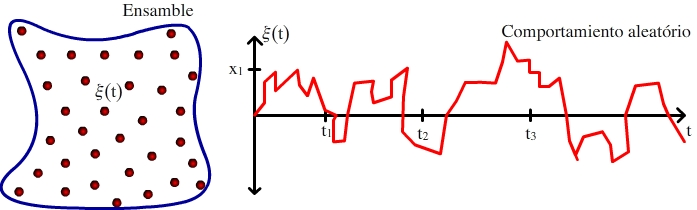
\includegraphics[width=0.5\textwidth]{aleatorio.jpg}
\caption{Esquematizaci\'on de un ensamble de sistemas f\'isicos que tiene asociado a \'el una cierta cantidad $\xi$ que se comporta de manera aleatoria con el tiempo.}
\label{fig:aleatorio}
\end{center}
\end{wrapfigure}

Comencemos considerando un ensamble de muchas part\'iculas en cuya din\'amica interviene una cantidad que var\'ia aleatoriamente y que es representada por la letra $\xi$. Supongamos adem\'as que esa cantidad $\xi$ depende del tiempo de forma tal que pueda describirse como una funci\'on de $t$, $\xi(t)$, tal como se representa en la figura \ref{fig:aleatorio}. En imposible predecir con absoluta certeza el comportamiento que mostrar\'a $\xi$ con el transcurrir del tiempo. Se acude entonces a lo que se acostumbra a hacer en estos casos y es trabajar con densidades de probabilidad.\\

Definimos la densidad de probabilidad de que $\xi(t_1)$ se encuentre entre el intervalo $x_1\leq\xi(t_1)\leq x_1+dx_1$, en donde $x_1\,\epsilon\,D(\xi)$, siendo $D(\xi)$ el conjunto dominio de los valores de $\xi$.

\begin{align}
W_1(x_1,t_1)=\langle\delta(x_1-\xi(t_1))\rangle,
\end{align}

\noindent donde con los s\'imbolos  $\langle\rangle$ se expresa un promedio sobre todo el ensamble. Ahora bien, en esta misma v\'ia se puede definir la densidad de probabilidad de que $\xi(t_1)$ se encuentre en el intervalo $x_1\leq\xi(t_1)\leq x_1+dx_1$ pero que tambi\'en $\xi(t_2)$ est\'e en $x_2\leq\xi(t_2)\leq x_2+dx_2$, ..., y que  $\xi(t_n)$ est\'e contenido en $x_n\leq\xi(t_n)\leq x_n+dx_n$ como

\begin{align}
W_n(x_n,t_n;...;x_1,t_1)=\langle\delta(x_1-\xi(t_1))...\delta(x_n-\xi(t_n))\rangle.
\end{align}

Supongamos ahora que conocemos una cierta cantidad de densidades de probabilidad jerarquizadas como sigue:

\begin{align}
&W_1(x_1,t_1)\\\nonumber
&W_2(x_1,t_1;x_2,t_2)\\\nonumber
&W_3(x_1,t_1;x_2,t_2;x_3,t_3)\\\nonumber
&...
\end{align}

\noindent para todo $t_i$ que se encuentre en el intervalo $t_0\leq t_i\leq t_0+T$. En otras palabras, lo que esto indica es suponer que se conoce la evoluci\'on temporal completa de la variable aleatoria $\xi(t)$. \\

La exigencia de conocer estas densidades de probabilidad de manera expl\'icita se hace con fin de poder definir formalmente los valores promedios de ciertas cantidades propias del sistema f\'isico bajo una simple integral, i.e. poderlas correlacionar entre s\'i. Por ejemplo, siendo $t'>t$, la correlaci\'on de la variable aleatoria entre dos diferentes tiempos se puede expresar como

\begin{align}
\langle\xi(t)\,\xi(t')\rangle=\int x\,...\,x'W'(x,t;...;x',t')\,dx\,...\,dx'.
\end{align}

{\bf Densidad de probabilidad restringida} (o condicionada): Basados en lo anterior podemos definir una densidad de probabilidad de la variable aleatoria $\xi$ para un tiempo $t_n$ bajo la condici\'on de que para un $t_{n-1}<t_n$ se tenga a certeza de que la variable aleatoria tom\'o el valor $x_{n-1}$, para $t_{n-2}<t_{n-1}$, $\xi(t_{n-2})=x_{n-2}$, y as\'i sucesivamente hasta que para $t_1<t_2$, $\xi(t_1)=x_1$. Formalmente,

\begin{align}
P(x_n,t_n|x_{n-1},t_{n-1};...;x_1,t_1)=\langle\delta(x_n-\xi(t_n))\rangle|_{\xi(t_{n-1})=x_{n-1},...,\xi_{t_1}=x_1}.
\end{align}\\

Esta misma densidad de probabilidad restringida se puede expresar en funci\'on de los $W_n$ como:

\begin{align}\label{pxn}
P(x_n,t_n|x_{n-1},t_{n-1};...;x_1,t_1)=\frac{W_n(x_n,t_n;...;x_1,t_1)}{W_{n-1}(x_{n-1},t_{n-1};...;x_1,t_1)},
\end{align}

\noindent pero dado que $W_{n-1}$ la podemos re-escribir como

\begin{align}
W_{n-1}(x_{n-1},t_{n-1};...;x_1,t_1)=\int W_n(x_n^*,t_n^*;...;x_1,t_1)\,dx_n^*,
\end{align}

\noindent (\ref{pxn}) toma la forma

\begin{align}
P(x_n,t_n|x_{n-1},t_{n-1};...;x_1,t_1)=\frac{W_n(x_n,t_n;...;x_1,t_1)}{\int W_n(x_n^*,t_n^*;...;x_1,t_1)\,dx_n^*};
\end{align}

\noindent de donde finalmente se deduce que

\begin{align}\label{wp}
W_n(x_n,t_n;...;x_1,t_1)=\int P(x_n,t_n|x_{n-1},t_{n-1};...;x_1,t_1)\,W_n(x_n^*,t_n^*;...;x_1,t_1)\,dx_n^*.
\end{align}\\

En general; si definimos un $x'=x+\varepsilon$, con $\varepsilon>0$, y como $t+\tau>t$, con $\tau>0$; podemos re-escribir (\ref{wp}) como

\begin{align}\label{wxt}
W(x',t+\tau)=\int P(x',t+\tau|x,t)\,W(x,t)\,dx,
\end{align}

\noindent siendo $P(x',t+\tau|x,t)$ la densidad de probabilidad de que ocurra la transici\'on de $x,\,t$ a $x',\,t+\tau$. Ahora bien, en la ecuaci\'on de {\it Fokker-Planck} interviene la derivada temporal de $W(x,t)$, $\partial W(X,T)/\partial t$, para lo cual es inherente conocer la probabilidad de transici\'on $P(x',t+\tau|x,t)$ para valores de $\tau$ peque\~nos, y en busca de una representaci\'on de esta derivada es que se trabaja a continuaci\'on.\\

Para empezar establecemos la suposici\'on de que es posible conocer todos los {\bf momentos} estad\'isticos de la distribuci\'on, esto es, que se conoce

\begin{align}
M_n(x,t,\tau)=\langle[\xi(t+\tau)-\xi(t)]^n\rangle |_{\xi(t)=x}=\int (x'-x)^nP(x',t+\tau|x,t)\,dt
\end{align}

\noindent para todo $n\,\epsilon\,\mathds{Z}$. Ahora bien, podemos hacer uso de la siguiente identidad general de los {\it deltas de Dirac}:

\begin{align}\label{pxp}
P(x',t+\tau|x,t)=\int\delta(y-x')\,P(y,t+\tau|x,t)\,dy,
\end{align}

\noindent y expresar $\delta(y-x')$ como $\delta(y-x+x-x')$.\\

Ahora, tratemos de expandir la funci\'on {\it delta de Dirac} en series de Taylor. La expresi\'on general para una expanci\'on en series de Taylor es

\begin{align}
f(x^*-x_0^*)=\sum_{n=0}^{\infty}\frac{f^{(n)}(x_0^*)}{n!}(x^*-x_0^*)^n.
\end{align}

\noindent Si, para nuestro caso, $x^*=(y-x)$, y, $x_0^*=(x'-x)$, as\'i

\begin{align}
\delta(y-x')&=\sum_{n=0}^\infty \frac{(y-x')^n}{n!}\left(\frac{\partial}{\partial x^*}\right)^n\delta(x'-x)\\\label{delta}
&=\sum_{n=0}^\infty \frac{(y-x')^n}{n!}\left(-\frac{\partial}{\partial x}\right)^n\delta(x'-x).
\end{align}

Introduciendo (\ref{delta}) en (\ref{pxp}) se tiene

\begin{align}
P(x',t+\tau|x,t)=\int\sum_{n=0}^\infty \frac{(y-x')^n}{n!}\left(-\frac{\partial}{\partial x}\right)^n\delta(x'-x)\,P(y,t+\tau|x,t)\,dy,
\end{align}

\noindent que sacando el primer t\'ermino de la suma se convierte en

\begin{align}
P(x',t+\tau|x,t)=\int\delta(x'-x)\,P(y,t+\tau|x,t)\,dy+\int\sum_{n=1}^\infty\frac{(y-x')^n}{n!}\left(-\frac{\partial}{\partial x}\right)^n\delta(x'-x)\,P(y,t+\tau|x,t)\,dy,
\end{align}

\noindent reacomodando t\'erminos:

\begin{align}
P(x',t+\tau|x,t)=\delta(x'-x)\,\underbrace{\int P(y,t+\tau|x,t)\,dy}_{\text{identidad}}+\sum_{n=1}^\infty\frac{1}{n!}\left(-\frac{\partial}{\partial x}\right)^n\delta(x'-x)\underbrace{\int(y-x)^n\,P(y,t+\tau|x,t)\,dy}_{M_n(x,t,\tau)},
\end{align}

\begin{align}
P(x',t+\tau|x,t)&=\delta(x-x')+\sum_{n=1}^\infty\frac{1}{n!}\left(-\frac{\partial}{\partial x}\right)^n\delta(x'-x)\,M_n(x,t,\tau),\\
&=\left[1+\sum_{n=1}^\infty\frac{1}{n!}\left(-\frac{\partial}{\partial x}\right)^n\,M_n(x,t,\tau)\right]\,\delta(x-x'),
\end{align}

\noindent donde se ha tenido en cuenta la identidad $\delta(x-x')=\delta(x'-x)$.\\

Insertando este \'ultimo resultado en (\ref{wxt}), tenemos

\begin{align}
W(x',t+\tau)&=\int P(x',t+\tau|x,t)\,W(x,t)\,dx\\
&=\int \left[1+\sum_{n=1}^\infty\frac{1}{n!}\left(-\frac{\partial}{\partial x}\right)^n\,M_n(x,t,\tau)\right]\,\delta(x-x')\,W(x,t)\,dx\\\label{ww}
&=W(x',t)+\sum_{n=1}^\infty\frac{1}{n!}\left(-\frac{\partial}{\partial x}\right)^n\int\delta(x-x')\,M_n(x,t,\tau)W(x,t)\,dx.
\end{align}

Por otro lado, cuando se considera el l\'imite en el que $\tau<<1$ 

\begin{align}
W(x',t+\tau)-W(x',t)=\frac{\partial W(x',t)}{\partial t}+\sigma(\tau^2),
\end{align}

\noindent en donde $\sigma(\tau^2)$ representa t\'erminos de orden superior a $\tau^2$; de esta manera, de (\ref{ww}) se tiene que

\begin{align}
W(x',t+\tau)-W(x',t)&=\sum_{n=1}^\infty\frac{1}{n!}\left(-\frac{\partial}{\partial x}\right)^n\int\delta(x-x')\,M_n(x,t,\tau)W(x,t)\,dx\\
\frac{\partial W(x',t)}{\partial t}&=\frac{1}{\tau}\sum_{n=1}^\infty\frac{1}{n!}\left(-\frac{\partial}{\partial x}\right)^n\int\delta(x-x')\,M_n(x,t,\tau)\,W(x,t)\,dx\\\label{wt}
&=\sum_{n=1}^\infty\frac{1}{n!}\left(-\frac{\partial}{\partial x'}\right)^n\,M_n(x',t,\tau)\,W(x',t).
\end{align}

Si se define $D^{(n)}(x',t)\equiv\frac{M_n(x',t,\tau)}{\tau\,(n!)}$, entonces (\ref{wt}) se generaliza como

\begin{align}
\boxed{\frac{\partial W(x',t)}{\partial t}=\sum_{n=1}^\infty\left(-\frac{\partial}{\partial x'}\right)^n\,D^{(n)}(x',t)\,W(x',t)}
\end{align}

\noindent que es la llamada {\it ecuaci\'on general de Kramer-Moyal} en una dimensi\'on.\\

Cuando la serie de {\it Kramer-Moyal} se trunca a segundo orden obtenemos la ecuaci\'on general de {\it Fokker-Planck} unidimensional:

\begin{align}
\boxed{\frac{\partial W(x,t)}{\partial t}=-\frac{\partial}{\partial x}[D^{(1)}(x,t)\,W(x,t)]+\frac{\partial^2}{\partial x^2}[D^{(2)}(x,t)\,W(x,t)]}
\end{align}

\subsection*{Ecuaci\'on de Fokker-Planck Multi-dimensional}
\addcontentsline{toc}{subsection}{Ecuaci\'on de Fokker-Planck Multi-dimensional}

Empecemos considerando un sistema de $N$ variables aleatorias $\{\xi\}=\{\xi_1,\xi_2,...,\xi_N\}$ para lograr extender la ecuaci\'on (\ref{wxt}) a 

\begin{align}\label{ro}
W(\{x'\},t+\tau)=\int P(\{x'\},t+\tau|\{x\},t)\,W(\{x\},t)\,d^Nx, 
\end{align}

\noindent donde el elemento de volumen es $d^Nx=dx_1\,dx_2\,...\,dx_N$ y el s\'imbolo integral resume las $N$ integrales que se deben hacer. A\'i mismo, $\{x\}$, $\{x'\}$ arriba (ecuaci\'on \ref{ro}), y en lo que sigue de esta secci\'on, representa al conunto ordenado de las respectivas variables. La funci\'on {\it delta} para estas $N$ variables es

\begin{align}
\delta(\{x\})=\delta(x_1)\,\delta(x_2)\,...\,\delta(x_N),
\end{align}

\noindent con lo que 

\begin{align}\label{si}
P(\{x'\},t+\tau|\{x\},t)=\int\delta(\{y\}-\{x'\})\,P(\{y\},t+\tau|\{x\},t)\,d^Ny.
\end{align}

Ahora trabajemos sobre la funci\'on $\delta(\{y\}-\{x'\})$ expandiendola en series \citep[]{aguirre2000},

\begin{align}
\delta(\{y\}-\{x'\})&=\delta(\{x\}-\{x'\}+\{y\}-\{x\})\\
&=\sum_{\nu=0}^\infty\frac{1}{\nu!}(y_{j1}-x_{j1})(y_{j2}-x_{j2})...(y_{j\nu}-x_{j\nu})\frac{\partial^\nu}{\partial x_{j1}\,\partial x_{j2}\,...\,\partial x_{j\nu}}\delta(\{x\}-\{x'\})\\\label{au}
&=\sum_{\nu=0}^\infty\frac{1}{\nu!}\frac{(-\,\partial)^\nu}{\partial x'_{j1}\,\partial x'_{j2}\,...\,\partial x'_{j\nu}}(y_{j1}-x_{j1})(y_{j2}-x_{j2})...(y_{j\nu}-x_{j\nu})\delta(\{x\}-\{x'\}),
\end{align}

\noindent donde se ha usado la notaci\'on de {\it suma} sobre los \'indices repetidos. Insertando (\ref{au}) en (\ref{si}), tenemos

\begin{align}\label{mi}
P(\{x'\},t+\tau|\{x\},t)=\left[1+\sum_{\nu=1}^\infty\frac{1}{\nu!}\frac{(-\,\partial)^\nu}{\partial x_{j1}\,\partial x_{j2}\,...\,\partial x_{j\nu}}M_{j_1,j_2,...,j_\nu}^{(\nu)}(\{x\},t,\tau)\right]\delta(\{x'\}-\{x\}),
\end{align}

\noindent donde se ha usado la definici\'on de {\it $\nu$-\'esimo} momento estad\'istico como

\begin{align}
M_{j_1,j_2,...,j_\nu}^{(\nu)}(\{x\},t,\tau)=\int(y_{j1}-x_{j1})(y_{j2}-x_{j2})\, ....\,(y_{j\nu}-x_{j\nu})\,P(\{y\},t+\tau|\{x\},t)\,d^Ny.
\end{align}

Llevando (\ref{mi}) a (\ref{ro}),

\begin{align}
W(\{x'\},t+\tau)&=\int \left[1+\sum_{\nu=1}^\infty\frac{1}{\nu!}\frac{(-\,\partial)^\nu}{\partial x_{j1}\,\partial x_{j2}\,...\,\partial x_{j\nu}}M_{j_1,j_2,...,j_\nu}^{(\nu)}(\{x'\},t,\tau)\right]\delta(\{x'\}-\{x\})\,W(\{x\},t)\,d^Nx,\\
W(\{x'\},t+\tau)-W(\{x'\},t)&=\sum_{\nu=1}^\infty\frac{1}{\nu!}\frac{(-\,\partial)^\nu}{\partial x_{j1}\,\partial x_{j2}\,...\,\partial x_{j\nu}}\int \delta(\{x'\}-\{x\})\,M_{j_1,j_2,...,j_\nu}^{(\nu)}(\{x\},t,\tau)\,W(\{x\},t)\,d^Nx,\\\label{lale}
\frac{\partial W(\{x'\},t)}{\partial t}&=\frac{1}{\tau}\sum_{\nu=1}^\infty\frac{1}{\nu!}\frac{(-\,\partial)^\nu}{\partial x'_{j1}\,\partial x'_{j2}\,...\,\partial x'_{j\nu}}\,M_{j_1,j_2,...,j_\nu}^{(\nu)}(\{x'\},t,\tau)\,W(\{x'\},t),
\end{align}

\noindent siento $\tau$ el intervalo de tiempo infinitesimal transcurrido entre $t$ y $t+\tau$.\\

Si definimos $D_{j_1,j_2,...,j_\nu}^{(\nu)}(\{x\},t)=\frac{M_{j_1,j_2,...,j_\nu}^{(\nu)}(\{x\},t,\tau)}{\tau\,(\nu!)}$, entonces (\ref{lale}) toma la forma m\'as general

\begin{align}
\boxed{\frac{\partial W(\{x'\},t)}{\partial t}=\sum_{\nu=1}^\infty\frac{(-\,\partial)^\nu}{\partial x'_{j1}\,\partial x'_{j2}\,...\,\partial x'_{j\nu}}\,D_{j_1,j_2,...,j_\nu}^{(\nu)}(\{x'\},t)\,W(\{x'\},t),}
\end{align}

\noindent conocida como la {\it ecuaci\'on de Kramer-Moyal multidimensional}. Cuando truncamos esta serie a segundo orden obtenemos la famosa ecuaci\'on de {\it Fokker-Planck} en varias variables:

\begin{align}\label{efp}
\boxed{\frac{\partial W(\{x\},t)}{\partial t}=-\,\frac{\partial}{\partial x_{j_1}}\,D_{j_1}^{2}(\{x\},t)\,W(\{x\},t)+\frac{\partial^2}{\partial x_{j_1}\,\partial x_{j_2}}\,D_{j_1\,j_2}^{2}(\{x\},t)\,W(\{x\},t),}
\end{align}

\noindent donde se usa la notaci\'on de suma sobre \'indices repetidos.

\subsection*{Ecuaci\'on de Fokker-Planck para una distribuci\'on de electrones que se inyecta en un plasma magnetizado}
\addcontentsline{toc}{subsection}{Din\'amica de un paquete de electrones que se inyecta en un plasma magnetizado}

La aceleraci\'on de electrones a altas energ\'ias es un fen\'omeno que se presenta en m\'ultiples escenerios astrof\'isicos como en los rayos c\'osmicos, en los jets de rayos gamma, en los n\'ucleos activos de galaxias, en los eventos de supernova y en las fulguraciones solares \citep[]{longair1992}. Con el advenimiento de la era moderna de la tecnolog\'ia y gracias a la extrema cercan\'ia del Sol con respecto a nosotros ha sido posible obtener una gran cantidad de datos observacionales (espectros e im\'agenes) de alta resoluci\'on espacial y temporal. Estas observaciones posibilitan la comparaci\'on detallada de los datos de ciencia con un an\'alisis te\'orico de la evoluci\'on temporal de la distribuci\'on electr\'onica mediante el empleo adecuado de la ecuaci\'on de {\it Fokker-Planck} como ecuaci\'on cin\'etica de movimiento del proceso en estudio. Es clara entonces la importancia de establecer los par\'ametros f\'isicos del medio en el cual se propagar\'an los electrones en la formulaci\'on te\'orica.\\

\begin{wrapfigure}[25]{l}{0.54\textwidth}
\begin{center}
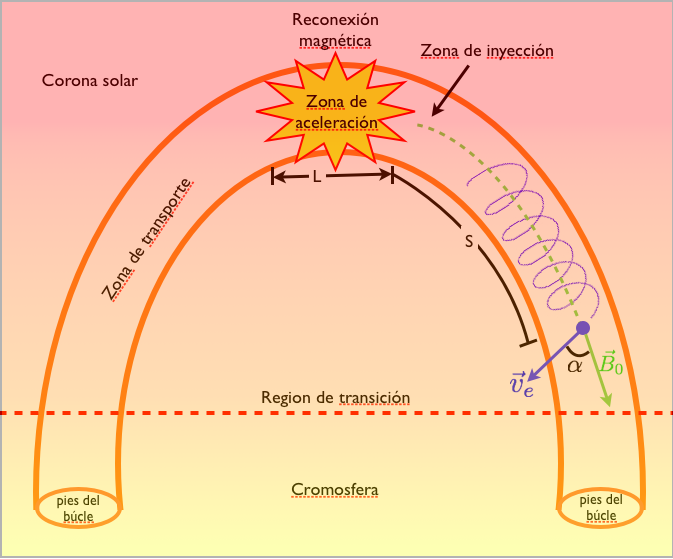
\includegraphics[width=0.53\textwidth]{pitchangle.png}
\caption{Esquematizaci\'on del giro-movimiento de una part\'icula cargada cuanto se transporta a lo largo de las l\'ineas de campo magn\'etico en el interior de un b\'ucle de plasma coronal.}
\label{fig:giromovimiento}
\end{center}
\end{wrapfigure}

B\'asicamente, durante las \'ultimas tres d\'ecadas se ha dado un avance importante en la construcci\'on de una descripci\'on te\'orica consistente que considere los procesos relevantes presentes en la interacci\'on del paquete de electrones en su viaje a trav\'es del plasma \citep[]{leach1981,bai1982,lu1988,mctiernan1990,hamilton1990,miller1996,1997park,liu2004,liu2009,zharkova2011a}.\\

Estos trabajos previos han mostrado que algunos de los procesos f\'isicos que causan que la distribuci\'on electr\'onica evolucione con el tiempo son la dispersi\'on {\it Coulombiana} y tipo {\it Compton}, la reflexi\'on magn\'etica, las interacciones tipo {\it onda-part\'icula}, la radiaci\'on sincrotr\'on, y los efectos directos de los campos el\'ectricos tipo DC, siendo los par\'ametros f\'isicos propios del plasma (tales como la densidad, la magnitud y topolog\'ia del campo magn\'etico y la energ\'ia y composici\'on de las part\'iculas) los factores que determinan cu\'ales de estos procesos predominan en el fen\'omeno.\\

La mayor\'ia de los plasmas astrof\'isicos se encuentran inmersos en un campo magn\'etico producto del movimiento de las part\'iculas cargadas que lo componen. Si en dichos plasmas la magnitud del campo magn\'etico predomina sobre la del campo el\'ectrico, el movimiento de las part\'iculas se hace principalmente a lo largo de las l\'ineas de $\vec{B}$ en lo que se conoce como {\it giro-movimiento} (ver figura \ref{fig:giromovimiento}). Este giro-movimiento se caracteriza por tres observables f\'isicos: la energ\'ia de la part\'icula en movimiento $E$, su posici\'on $s$, y el \'angulo de cabeceo $\alpha$; o en ingl\'es {\it pitch angle}, el cual se refiere al \'angulo formado entre el vector momentum de la part\'icula $\vec{p}$ en un instante dado y el vector campo magn\'etico $\vec{B}$ del lugar.\\

Si sobre uno de estos plasmas se inyecta un n\'muero grande de part\'iculas cargadas (por ejemplo electrones) con una distribuci\'on dada $W$, la din\'amica de estas, la evoluci\'on de sus movimientos, se podr\'a describir como se mostr\'o en la secci\'on anterior. En este caso, consideremos nuestra funci\'on de distribuci\'on $W$ como una funci\'on que depende de la energ\'ia $E$, la posici\'on de la part\'icula $s$ en la regi\'on, y del coseno del \'angulo de cabeceo $\mu$. As\'i, $W=W(E,\mu,s,t)$, y los c\'alculos pertinentes se llevar\'an a cabo en el espacio de fases. 

En este caso la ecuaci\'on de {\it Fokker-Planck} (\ref{efp}) toma la forma:

\begin{align}\label{eq:fph}
\frac{\partial W}{\partial t}=-\text{v}\mu\frac{\partial W}{\partial s}-\frac{\partial}{\partial \mu}(\dot{\mu}W)-\frac{\partial}{\partial E}(\dot{E}W)+\frac{\partial}{\partial\mu}\left(D_{\mu\mu}\frac{\partial W}{\partial\mu}\right)+\frac{\partial}{\partial E}\left(D_{EE}\frac{\partial W}{\partial E}\right)+\frac{\partial}{\partial E}\left(D_{E\mu}\frac{\partial W}{\partial\mu}\right)+\frac{\partial}{\partial\mu}\left(D_{E\mu}\frac{\partial W}{\partial E}\right).
\end{align}

Los coeficientes $\text{v}\cos\alpha$, $\dot{\mu}$ y $\dot{E}$ son los cambios sistem\'aticos en posici\'on, \'angulo de cabeceo y energ\'ia, respectivamente, producto de las fuerzas externas que act\'uan directamente sobre las part\'iculas en movimiento. Las cantidades $D_{j_1j_2}$ est\'an asociadas directamente con los diferentes procesos de dispersi\'on y por eso hacen parte de los t\'erminos difusivos de la expresi\'on \citep[]{hamilton1990}. Las formas expl\'icitas de los coeficientes $\dot{E}$, $\dot{\mu}$ y $D_{j_1j_2}$ para un conjunto de electrones bajo la influencia de colisiones tipo Coulomb, dispersiones Compton y de interacci\'on onda-part\'icula, radiaci\'on sincrotr\'on, variaciones del campo magn\'etico, y fuerzas externas son resumidas en las siguientes dos tablas \citep[]{hamilton1990}:

\begin{table}[htdp]
\caption{Tasas de cambio de la energ\'ia y el \'angulo de cabeceo. $\ln\Lambda$ es el logaritmo Coulombiano.}
\begin{center}
\begin{tabular}{|c|c|c|}\hline\hline
Proceso  & $\dot{E}$ & $\dot{\mu}$ \\\hline & & \\
Colisi\'on Coulombiana & $-4\pi ncr_0^2\ln\Lambda/\beta$ & 0 \\ & & \\
Emisi\'on sincrotr\'on & $-\frac{2}{3}B^2\gamma^2\beta^2(1-\mu^2)/mc$ & $-\frac{2}{3}r_0^2B^2\mu(1-\mu^2)/mc\gamma$ \\ & & \\
Fuerzas externas & $\mu\beta\,\mathbf{F}_{||}/mc$ & $(1-\mu^2)\mathbf{F}_{||}/\gamma\beta mc$ \\ & & \\
Reflejo magn\'etico & 0 & $-\frac{1}{2}\beta c(1-\mu^2)(d\ln B/ds)$ \\ & & \\
Ondas de Alfv\'en & $(1/\gamma\beta^2)(1-\beta^2)D_{EE}^{\text{Alfv\'en}}$ & $(1/\gamma\beta^2)(1+\beta^2)D_{E\mu}^{\text{Alfv\'en}}$ \\ & & \\
Ondas de Langmuir & $(1/\gamma\beta^2)(1-\beta^2)D_{EE}^{\text{Langmuir}}$ & 0 \\ & & \\\hline
\end{tabular}
\end{center}
\label{procesos}
\end{table}%

\begin{table}[htdp]
\caption{Coeficientes de difusi\'on}
\begin{center}
\begin{tabular}{|c|c|c|c|}\hline\hline
Coeficientes & Colisi\'on Coulombiana & Ondas de Alfv\'en & Ondas de Langmuir \\\hline & & & \\
$D_{\mu\mu}$ & $\frac{4\pi ncr_0^2\ln\Lambda}{\beta^2\gamma^2}(1-\mu^2)$ & $D_{-}^{(2)}+D_{+}^{(2)}$ & 0 \\ & & & \\
$D_{EE}$ & $\sim0$ & $\beta^4\gamma^2\frac{v_A^2}{v^2}(D_{-}^{(0)}+D_{+}^{(0)})$ & $\frac{ncr_0^2\epsilon_L}{\beta}\overline{k^{-3}}$ \\ & & & \\
$D_{E\mu}$ & $\sim0$ & $\beta^4\gamma^2\frac{v_A}{v}(D_{-}^{(1)}+D_{+}^{(1)})$ & 0 \\ & & & \\\hline
\end{tabular}
\end{center}
\label{difusion}
\end{table}%

En general, para la aceleraci\'on estoc\'astica de un conjunto de part\'iculas cargadas asociada a un proceso de fulguraci\'on solar, \cite{lu1988} mostraron que la ecuaci\'on (\ref{eq:fph}) toma la forma particular

\begin{align}\label{fph}
\frac{\lambda_0}{\text{v}}\frac{\partial W}{\partial t}=-\lambda_0\mu\frac{\partial W}{\partial s}+\lambda_0\frac{d\,\ln\,B}{ds}\frac{\partial}{\partial \mu}\left[\frac{(1-\mu^2)}{2}W\right]+\frac{c^2}{\text{v}}\frac{\partial}{\partial E}\left(\frac{W}{\text{v}}\right)+\frac{c^4}{\text{v}^4\gamma^2}\frac{\partial}{\partial \mu}\left[(1-\mu^2)\frac{\partial W}{\partial \mu}\right]+\frac{\lambda_0}{\text{v}}S(E,\mu,s,t),
\end{align}

\noindent donde $\lambda_0(s)=(10^{24\,\text{cm}})/n(s)\,\ln\Lambda$ es una cantidad que est\'a relacionada con el camino libre medio de un electr\'on que tienen una energ\'ia $E$  a trav\'es de la relaci\'on $\lambda(E)=\lambda_0\,E^2/(E+1)$. $n(s)$ es la densidad de n\'umero de part\'iculas del plasma en el ambiente en el cual se propaga el electr\'on.\\

Un an\'alisis completo y deductivo de modelamientos que se han hecho considerando algunos de estos tipos de interacciones se encuentran en \citep[]{petrosian1981,leach1981,petrosian1985,mctiernan1989,mctiernan1990,hamilton1990,somov1,ls1993,petrosian1994,Holman2001}. Sin embargo, en el cap\'itulo siguiente se muestra un revisi\'on ligera de los {\it tres} mecanismos que se consideran en el desarrollo del presente trabajo.\\

\section*{Procesos relevantes involucrados en las colisiones en plasmas}
\addcontentsline{toc}{section}{Procesos relevantes involucrados en las colisiones en plasmas}


\subsection*{Colisi\'on Coulombiana}
\addcontentsline{toc}{subsection}{Colisi\'on Coulombiana}

Tenemos que encargarnos de comprender cada una de las diferentes interacciones que se quieren considerar para el modelamiento de la interacci\'on del jet de electrones con el plasma de la atm\'osfera solar. El primer proceso que vemos en las tablas (\ref{procesos}) y (\ref{difusion}) es la colisi\'on entre part\'iculas tipo Coulomb. Esto se debe a que en general una part\'icula que incide velozmente sobre un plasma tiene colisiones con los electrones at\'omicos y con los n\'ucleos que lo componen. Los electrones del plasma, al ser ligeros, pueden adquirir una cantidad de energ\'ia apreciable por parte de los electrones incidentes sin provocar desviaciones importantes en la direcci\'on de su movimiento; mientras que, los n\'ucleos, de mayor masa, absorben muy poca energ\'ia; pero, en cambio, por efecto de su carga, provocan dispersiones notables a las part\'iculas incidentes. Una pregunta que se evidencia en las m\'ultiples explicaciones que se tratan de dar en cuanto al sistema de generaci\'on de sismos asociados a fulguraciones solares es: Si los electrones al poseer menor masa se ven m\'as alterados en su trayectoria y tienden a difundirse en su camino, c\'omo es que logran tener alcances tan profundos de la atm\'osfera solar para eventualmente estar asociados a la generaci\'on de la fuente s\'ismica? Este es uno de los mayores contra-argumentos que se dan al intentar de proponer un modelo como el nuestro, pero que algunos autores tratan de responder atribuyendo esta capacidad de penetraci\'on a la enorme cantidad de energ\'ia adquirida en el momento de la explosi\'on y posteriormente en el proceso de aceleraci\'on \citep[]{zharkova2011a}.\\

\begin{figure}[ht!]
\begin{center}
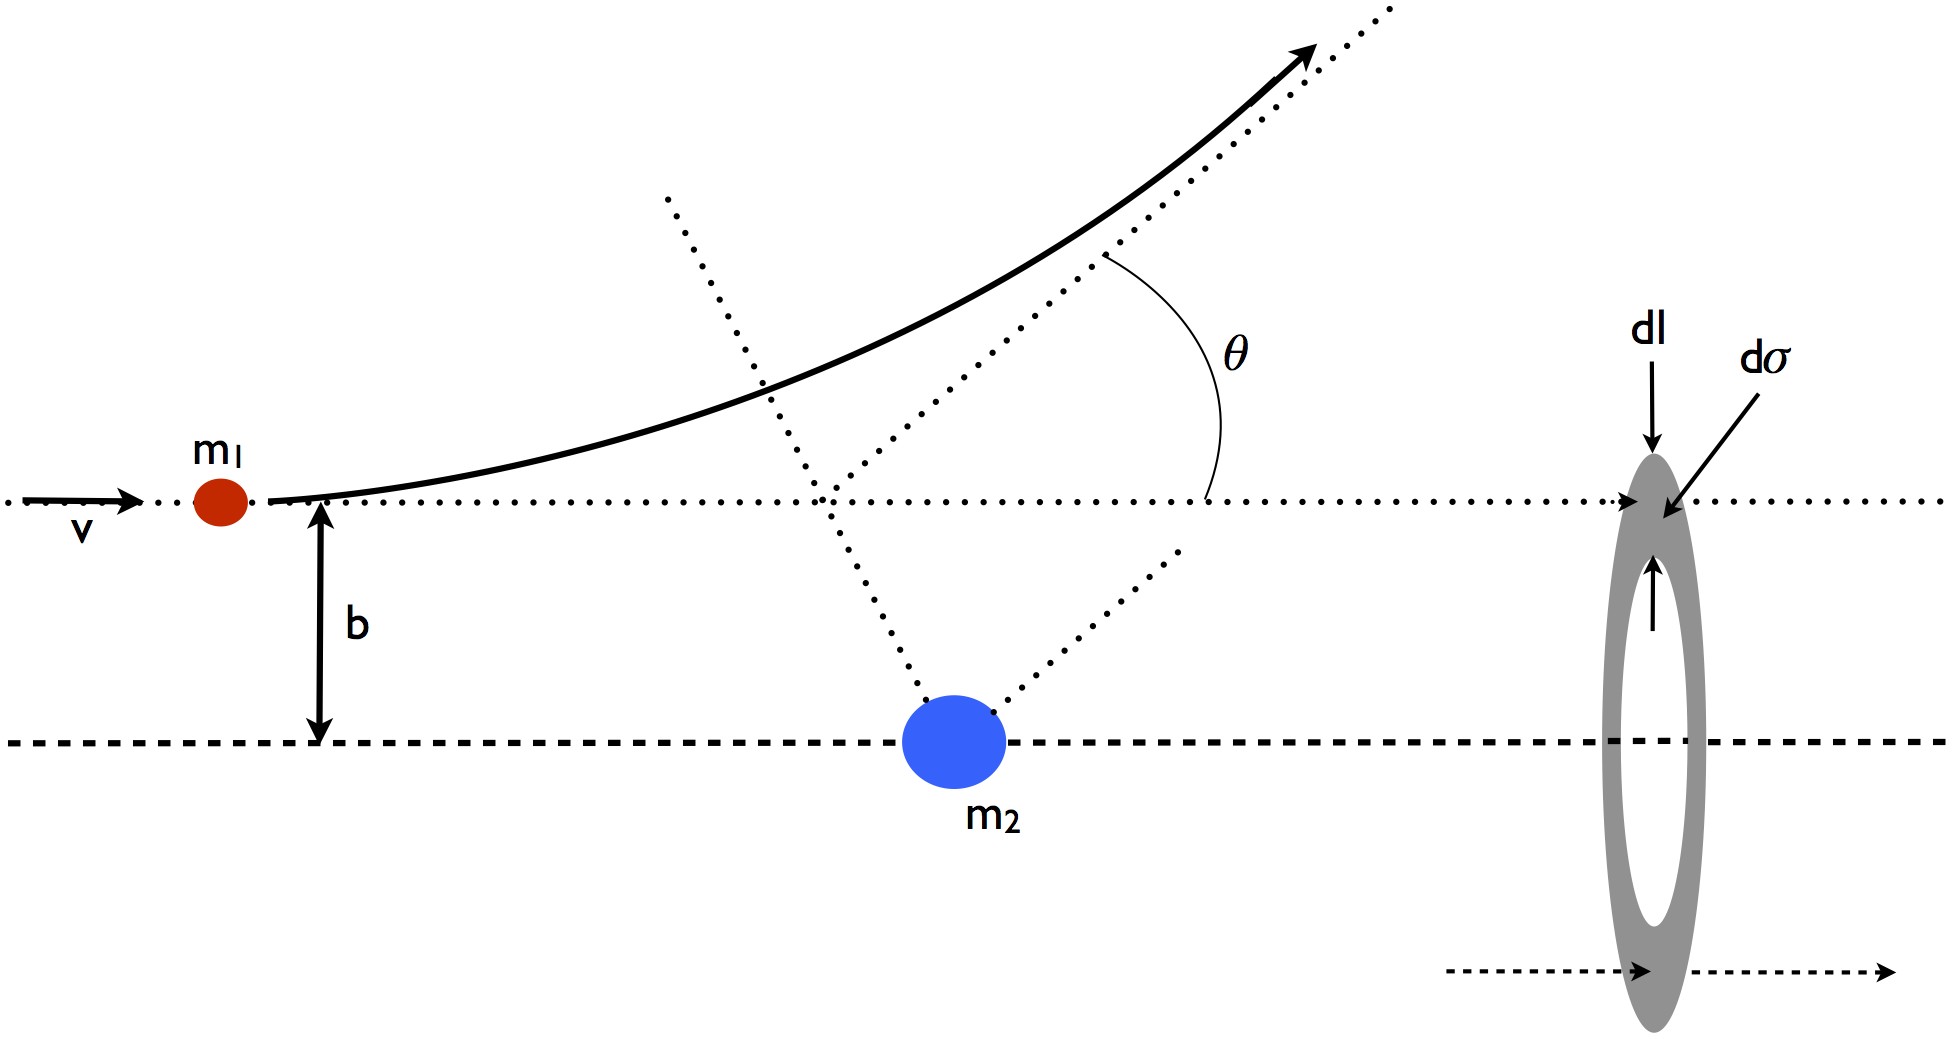
\includegraphics[width=0.73\textwidth]{coulomb.png}
\caption{Esquematizaci\'on de la interacci\'on de dos part\'iculas el\'ectricamente cargadas mediante un potencial {\it coulombiano}. Ilustraci\'on de los conceptos de par\'ametro de impacto y secci\'on eficaz.}
\label{fig:coulomb}
\end{center}
\end{figure}


La colisi\'on de dos part\'iculas relacionadas mediante un potencial {\it Coulombiano}, $\phi=e/r$, genera intercambios de momentum y de energ\'ia, y por tanto p\'erdidas cuando nos centramos en una part\'icula que incide sobre otra, ambas con una carga el\'ectrica asociada. Esta interacci\'on se esquematiza en la figura \ref{fig:coulomb}.\\

Si consideramos un sistema de referencia cuyo origen se encuentre en el centro de masa del sistema de las dos part\'iculas, cada una de las part\'iculas se dispersa un \'angulo $\theta$ definido por la relaci\'on

\begin{align}\label{theta1}
\tan\frac{\theta}{2}=\frac{e_1e_2}{\mu \text{v}^2b},
\end{align}

\noindent donde $\mu=\frac{m_1m_2}{m_1+m_2}$ es la masa reducida del sistema, $e_1$ y $e_2$ son las cargas respectivas de cada una de las part\'iculas, v es la velocidad inicial relativa de la part\'icula incidente y $b$ es el {\it par\'ametro de impacto} de la interacc\'on. Para ver una deducci\'on formal de la expresi\'on (\ref{theta1}) \citep[]{landau-mecanica}. Ahora bien, para una part\'icula que se deflecta un \'angulo de $\pi/2$

\begin{align}
b\left(\frac{\pi}{2}\right)=b_{\perp}=\frac{e_1e_2}{\mu \text{v}^2},
\end{align}

\noindent de manera que podemos escribir (\ref{theta1}) como

\begin{align}
\tan\frac{\theta}{2}=\frac{b_\perp}{b}.
\end{align}

Se habla entonces de una colisi\'on cercana si 

\begin{align}
\pi/2\leq\theta\leq\pi,\qquad\text{i.e.}\qquad0\leq b\leq b_\perp,
\end{align}

\noindent correspondientemente se tiene que, una colisi\'on lejana ser\'a aquella para la cual $b>b_\perp$ y $0\leq\theta\leq\pi/2$. Los dos casos pueden ser comprendidos a trav\'es de la figura \ref{fig:coulomb}.\\

Cada nueva colisi\'on provoca un peque\~no cambio en la cantidad de momentum perpendicular de las part\'iculas dado por

\begin{align}\label{tos}
\Delta p_\perp=p\sin\theta=m_1\text{v}_1\frac{2\tan\theta/2}{1+\tan^2(\theta/2)}=\frac{2m_1\text{v}_1(b_\perp/b)}{1+(b_\perp/b)^2}=2m_1\text{v}_1\frac{x}{1+x^2},
\end{align}


\noindent donde se ha definido $x=b_\perp/b$, y $0<\sin\theta\leq1$. La desigualdad anterior es estricta en el valor inferior, ya que como se ver\'a m\'as adelante al realizar la integraci\'on, considerar el caso nulo en $\sin\theta$ nos conducir\'ia a una divergencia. Esto implica que debemos considerar un $\theta_{min}$ correspondiente a un $b_{max}$. Ya que la variable $b$ toma valores aleatorios, se debe trabajar con una tasa media de cambio promediada bajo la probabilidad de interacci\'on asociada a la {\it secci\'on eficaz} $\sigma$:

\begin{align}
\frac{d}{dt}p_\perp^2=\int_{\theta=\pi/2}^{\theta=\theta_{min}}(\Delta p_\perp)^2\,n_2\,\text{v}_1\,d\sigma,
\end{align}

\noindent donde $n_2$ es la densidad de n\'umero de part\'iculas de la especie 2. Reemplazando aqu\'i la \'ultima expresi\'on de (\ref{tos}) y la expresi\'on de la secci\'on eficaz diferencial, se tiene que

\begin{align}\label{integral}
\frac{d}{dt}p_\perp^2=8\pi\,n_2\,m_1^2\,\text{v}_1^3\,b_\perp^2\int_{1}^{x_{min}}\frac{dx}{(1+x^2)^2x},
\end{align}


\noindent en donde $x_{min}$ es igual a $b_\perp/b_{max}$. Evaluando la integral en (\ref{integral}) mediante el empleo tradicional del m\'etodo de fracciones parciales, se encuentra que 

\begin{align}
\int_{1}^{x_{min}}\frac{dx}{(1+x^2)^2x}=\left[\ln x-\frac{1}{2}\ln(1+x^2)+\frac{1}{2(1+x^2)}\right]_{x=1}^{x=x_{min}}
\end{align}

Al evaluar esta integral en el l\'imite inferior obtenemos un valor muy peque\~no que resulta esp\'ureo en nuestros c\'alculos. Cuando se trata de evaluar esta misma integral pero en un valor muy cercano a cero (como es el caso del l\'imite superior) los t\'erminos que predominan son los que contienen logaritmos, as\'i

\begin{align}
\left[\ln x-\frac{1}{2}\ln(1+x^2)+\frac{1}{2(1+x^2)}\right]_{x=x_{min}}\approx\ln\left[\frac{1}{\sqrt{1+\frac{1}{x^2}}}\right]_{x_{min}}\sim\ln\frac{1}{x_{min}}=\ln\frac{b_{max}}{b_\perp},
\end{align}
 
\noindent Es usual definir un par\'ametro adimensional $\Lambda$ mediante:

\begin{align}
\Lambda=b_{max}/b_\perp,
\end{align}

\noindent conocido en la literatura como el {\it logaritmo Coulombiano} y que en el caso general en el que se considera equilibrio termodin\'amico se expresa mediante \citep[]{somov1}

\begin{align}
\ln\Lambda=\ln\frac{3}{2e^2}\left(\frac{k_B^3T^3}{\pi\,n_e}\right)^{1/2}.
\end{align}

Entonces finalmente (\ref{integral}) se puede aproximar como 

\begin{align}
\frac{d}{dt}p_\perp^2=8\pi\,n_2\,m_1^2\,\text{v}_1^3\,b_\perp^2\,\ln\Lambda.
\end{align}

Al normalizar con la energ\'ia cin\'etica de la part\'icula $1$, ($\frac{1}{2}m_1v_1^2$) tenemos una forma general del coeficiente de deriva involucrado en la ecuaci\'on de {\it Fokker-Planck} al considerar procesos de colisi\'on Coulombiana como es el caso de las fulguraciones solares en donde hoy en d\'ia se cree ampliamente que es la radiaci\'on {\it Bremsstrahlung} por colisi\'on Coulomb la principal responsable de la emisi\'on en rayos-X asociadas a este tipo de eventos \citep[]{leach1983}. Tambi\'en, es ampliamente aceptado que la mayor contribuci\'on de la emisi\'on en radio-frecuencias asociada a una fulguraci\'on es debida a la emisi\'on {\it girosincrotr\'on} \citep[]{zharkova2011a} y es por esto que es uno de los procesos con mayor importancia en el desarrollo te\'orico que en este trabajo se presenta y la raz\'on de la siguiente subsecci\'on.

\subsection*{Radiaci\'on giro-sincrotr\'on}
\addcontentsline{toc}{subsection}{Radiaci\'on giro-sincrotr\'on}

Toda part\'icula cargada que se acelera emite radiaci\'on electromagn\'etica; y si adem\'as la trayectoria que describe la part\'icula en su movimiento es circular, entonces a la radiaci\'on de le llama {\it radiaci\'on de sincrotr\'on}. La primera evidencia experimental de este tipo de radiaci\'on se dio en 1947 en el acelerador de electrones de la General Electric en el estado de Nueva York \citep[]{Elder1947}. Un desarrollo te\'orico completo de este fen\'omeno fue presentado por {\it Joseph Larmor} en 1898 en donde presenta explicitamente una expresi\'on que da cuenta de la potencia de radiaci\'on:

\begin{align}
P=\frac{e^2}{6\pi\varepsilon_0c^3}a^2
\end{align}


\noindent en donde $e$ es la carga de la part\'icula, $\varepsilon_0$ es al permitividad el\'ectrica del medio en el que la part\'icula se propaga, $c$ es la velocidad de la luz en el medio y $a$ es la acelaraci\'on centr\'ipeta (esta potencia es evaluada en todos los $4\pi$ estereoradianes de \'angulo s\'olido) \citep[]{Larmor1898}. En los aceleradores de part\'iculas es penas natural esperar encontrar este tipo de radiaci\'on, pues las trayectorias de las part\'iculas est\'an confinadas al arreglo circular que en si mismo es el acelerador. La pregunta que de inmediato se desprende en el marco de este trabajo es \textinterrobangdown C\'omo puede esta radiaci\'on estar asociada a un evento de fulguraci\'on solar? Pues bien, hoy en d\'ia se entiende que la mayor parte de la fenomenolog\'ia observada en la superficie del Sol est\'a regida por la presencia de intensos campos magn\'eticos, y como ya se mencion\'o con anterioridad las fulguraciones solares, en si mismas, son eventos producto de una reconexi\'on magn\'etica. La fuerza de Lorentz en presencia exclusiva de un campo magn\'etico,

\begin{align}
\vec{F}_L=\frac{e}{c}\,[\vec{\text{v}}\times \vec{B}],
\end{align}

\noindent es una fuerza que se aplica siempre en direcci\'on perpendicular al movimiento inst\'antaneo de la part\'icula. Los modelos de fulguraci\'on plantean un movimiento como el que se esquematiza en la figura \ref{fig:helicoide} \citep[]{1997park,white2011,zharkova2011a}.

\begin{figure}[ht!]
  \centering
  \subfloat[]{\label{fig:giro1}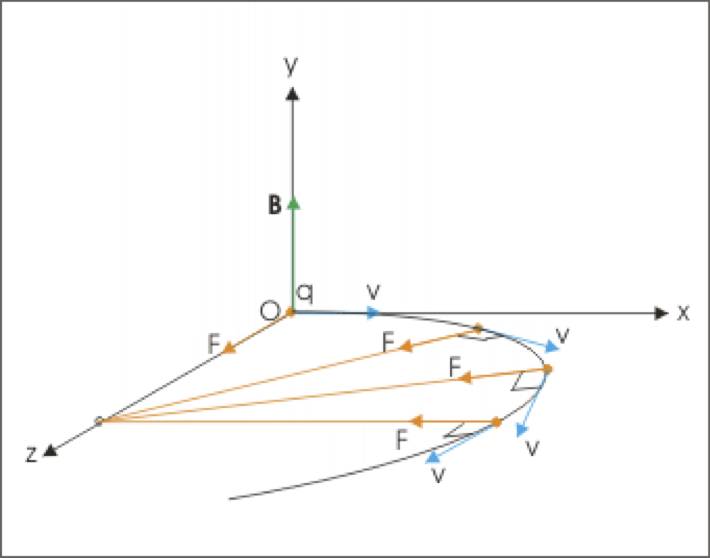
\includegraphics[width=0.45\textwidth]{giro1.png}}
  \hspace{0.3cm}
  \subfloat[]{\label{fig:giro2}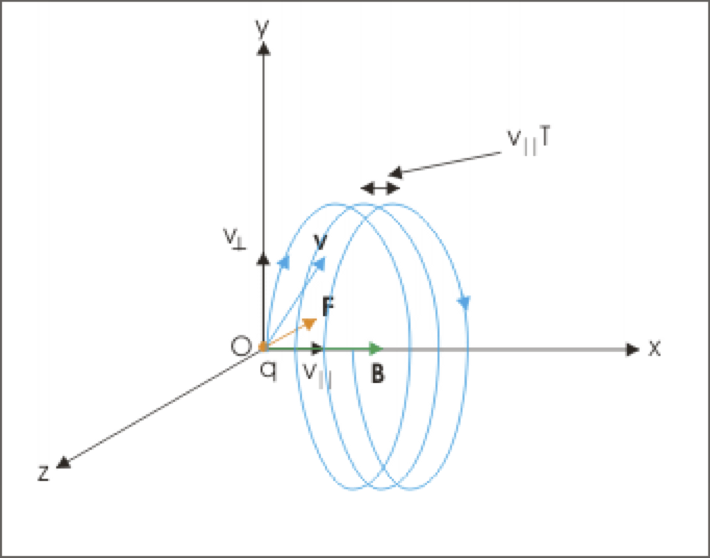
\includegraphics[width=0.45\textwidth]{giro2.png}}
  \caption{Esquematizaci\'on de la direcci\'on de la fuerza de Lorentz magn\'etica que se aplica sobre una part\'icula cargada en movimiento. (a) Un campo magn\'etico dirigido en la direcci\'on de $y$ y una part\'icula con carga $q$ que inicialmente tiene una velocidad $\vec{\text{v}}$ dirigida en direcci\'on $x$. El movimiento de esta part\'icula se es una circunferencia confinada en el plano $xz$. (b) Una trayectoria helicoidal se puede dar solamente en el caso en el que la fuerza neta que actua sobre la part\'icula cargada tenga una componente en la direcci\'on del campo magn\'etico como en el plano perpendicular a \'el. Imagenes tomadas de Singh, S. Motion of a charged particle in magnetic field, Connexions Web site. http://cnx.org/content/m31345/1.9/, Marzo 24, 2012.}
  \label{fig:helicoide}
\end{figure}

Para analizar en detalle la emisi\'on electromagn\'etica producto de este movimiento helicoidal de una part\'icula cargada es necesario considerar la forma en que los campos el\'ectricos y magn\'eticos se ven afectados y, por ende, la forma en la que una se\~nal electromagn\'etica es transmitida. Para desarrollar este an\'alisis se necesita apelar a los conocidos potenciales retardados de {\it Li\'enard-Wiechert} en donde despu\'es de algunas consideraciones f\'isicas y un extensivo desarrollo algebraico (ver por ejemplo \citep[]{jackson1975} o \citep[]{Schwartz1987}) se llega a una expresi\'on que da cuenta de la potencia energ\'etica radiada por unidad de \'angulo s\'olido como:

\begin{align}\label{eq:pot}
\frac{dP}{d\Omega}=\frac{e^2a^2}{4\pi c^3}\frac{(1-\beta \cos\theta')^2-(1-\beta^2)\sin^2\theta'\cos^2\varphi}{(1-\beta\cos\theta')^5}
\end{align}

\noindent donde nuevamente $e$ es la carga de cada part\'icula, $a$ es aceleraci\'on centr\'ipeta, $c$ es la velocidad de porpagaci\'on de una onda electromagn\'etica en el medio, $\beta$ es la velocidad de la part\'icula (en unidades de $c$), $\theta'$ es el \'angulo de polar (diferente al \'angulo de cabeceo descrito anteriormente) y $\varphi$ es el \'angulo axial. La potencia total radiada se encuentra al integrar la relaci\'on (\ref{eq:pot}) en el \'angulo s\'olido \citep[]{Schwartz1987}:

\begin{align}\label{P4pi}
P=\int_{4\pi} \frac{dP}{d\Omega}\,d\Omega=\frac{2e^2a^2}{3c^3}\frac{1}{(1-\beta^2)^2}=\frac{2e^2a^2}{3c^3}\gamma^4.
\end{align}

Si se considera que la part\'icula cargada est\'a inmersa en un campo magn\'etico predominantemente unidireccional ser\'a la fuerza de Lorentz la asociada a la aceleraci\'on centr\'ipeta que gobierna el movimiento circular en el helicoide

\begin{align}
F=\gamma ma=\frac{e\text{v}B\sin\theta}{c}
\end{align}

\noindent de donde se despeja $a$ como

\begin{align}\label{avB}
a=\frac{e\text{v}B\sin\theta}{\gamma mc},
\end{align}

\noindent siendo $m$ la masa de la part\'icula en su sistema {\it pr\'opio} de referencia. Llevando (\ref{avB}) en (\ref{P4pi}) tenemos:

\begin{align}
P=\frac{2e^2\gamma^4}{3c^3}\frac{e^2\beta^2B^2\sin^2\theta}{\gamma^2m^2}=\frac{e^4}{mc^2}\frac{2}{3}\frac{B^2\gamma^2\beta^2(1-\cos^2\theta)}{mc},
\end{align}

\noindent que resulta ser la expresi\'on que aparece en la tabla \ref{procesos} que da cuenta de la perdida de energ\'ia v\'ia radiaci\'on de sincrotron midiendo la carga en unidades de la carga del electr\'on y la energ\'ia medida en unidades de la energ\'ia en reposo del electr\'on $mc^2$. Todos estos procesos involucrados en el choque de un plasma son considerados en este trabajo pues nuestra finalidad es tratar de dar una explicaci\'on razonable de la forma en la que la fuente sismica es generada en aquellos eventos ac\'usticos observados asociados a eventos de fulguraci\'on solar y que es la materia que hoy en d\'ia conforma la rama conocida como la {\it Heliosismolog\'ia local} que ser\'a el tema que trataremos a continuaci\'on.


\subsection*{Reflexi\'on magn\'etica}
\addcontentsline{toc}{subsection}{Reflexi\'on magn\'etica}


Seg\'un los modelos actuales, la distribuci\'on de l\'ineas de campo magn\'etico a lo largo de un bucle solar es algo como lo que se representa en la figura \ref{fig:bucle}, en donde la densidad de l\'ineas aumenta progresivamente de forma sim\'etrica a partir de la cima del bucle y a medida que se avanza hacia las bases de \'el. Si se supone que la configuraci\'on de campo magn\'etico es tal que no varia con el tiempo, entonces cualquier part\'icula cargada el\'ectricamente que se mueva en una trayectoria helicoidal desde la cima del bucle en direcci\'on hacia alguna de sus bases sufrir\'a una reflex\'ion en un punto debido justamente al aumento progresivo de la densidad de l\'ineas de campo magn\'etico. Para entender esto desde un punto de vista formal, debemos empezar por recordar el concepto de invarianza adiab\'atica de algunas cantidades asociadas a un sistema f\'isico din\'amico.\\

El teorema de la invarianza adiab\'atica implica que las integrales de acci\'on no var\'ian cuando se produce un cambio que es lo suficientemente lento comparado con los periodos de movimiento del sistema f\'isico y adem\'as dichos cambios no set\'an relacionados de forma alguna con los periodos. Sea $q_i$ el conjunto de coordenadas generalizadas del sistema donde $i$ indexa a cada una de estas variables, y $p_i$ los momentos can\'onicos conjugados generalizados de cada una de las variables respectivamente. Toda coordenada peri\'odica define una integral de acci\'on

\begin{align}
J_i=\oint p_i\,dq_i.
\end{align}

El movimiento transversal de una part\'acula cargada en un campo magn\'etico est\'atico es un movimiento peri\'odio, de manera que se puede definir la integral de acci\'on siguiente

\begin{align}\label{eq:j}
\vec{J}=\oint \vec{P}_\perp\cdot d\vec{l},
\end{align}

\noindent donde $\vec{P}_\perp$ es la componente del momentum magn\'etico que es perpendicular a las l\'ineas de campo magn\'etico en cada punto, y $d\vec{l}$ es la diferencial de longitud a lo largo del c\'irculo instant\'aneo de la part\'icula definido en su \'orbita helicoidal a lo largo de las l\'ineas de campo magn\'etico que es justamente el camino sobre el cual se eval\'ua la integral. El vector momentum $\vec{P}$ es

\begin{align} 
\vec{P}=\gamma m\vec{\text{v}}+\frac{e}{c}\vec{A},
\end{align}

\noindent de manera que reemplazando expl\'icitamente en la ecuaci\'on (\ref{eq:j}) tenemos

\begin{align}\label{eq:j1}
\vec{J}=\oint\gamma m\vec{\text{v}}_\perp\cdot d\vec{l}+\frac{e}{c}\oint\vec{A}\cdot d\vec{l}.
\end{align}

De la primera integral de la ecuaci\'on (\ref{eq:j1}) se tiene que

\begin{align}
\vec{\text{v}}\cdot d\vec{l}&=(\omega_B\,a\,\hat{\theta})\cdot(a\,d\theta\,\hat{\theta})\\
&=\omega_B\,a^2\,d\theta,
\end{align}

\noindent siendo $\vec{a}$ el radio instant\'aneo descrito por la \'orbita de la part\'icula, $\omega_B$ la frecuencia angular (conocida tambi\'en como {\it frecuencia de Larmor} definida por $\omega_B=\frac{eB}{\gamma mc}$) y $\theta$ el \'angulo barrido sobre la circunferencia. De esta manera (\ref{eq:j1}) se re-escribe como

\begin{align}
\vec{J}=\oint\gamma\, m\,\omega_B\, a^2\,d\theta+\frac{e}{c}\oint\vec{A}\cdot d\vec{l};
\end{align}

\noindent aplicamos el teorema de {\it Stokes} sobre este t\'ermino

\begin{align}
\vec{J}=\oint\gamma\,m\,\omega_B\,a^2\,d\theta-\frac{e}{c}\int_S(\vec{\nabla}\times\vec{A})\cdot\hat{n}\,da,
\end{align}

\noindent en donde $S$ es la superficie encerrada por la circunferencia instant\'anea de la trayectoria de la part\'icula, y el signo negativo del segundo t\'ermino aparece porque el vector unitario $\hat{n}$ se dirige en sentido contrario a las l\'ineas de campo magn\'etico. De esta manera,

\begin{align}
\vec{J}&=\oint\gamma\,m\,\omega_B\,a^2\,d\theta-\frac{e}{c}\int_S\vec{B}\cdot\hat{n}\,da\\\label{eq:j2}
&=2\pi\,\gamma\,m\,\omega_B\,a^2+\frac{e}{c}\,|\vec{B}|\,\pi\,a^2.
\end{align}

Reemplazando expl\'incisamente la frecuencia de Larmor en (\ref{eq:j2}), tenemos

\begin{align}
\vec{J}=\gamma\,m\,\omega_B\,\pi\,a^2=\frac{e}{c}\,\underline{(B\,\pi\,a^2)},
\end{align}

\noindent en donde el \'ultimo t\'ermino entre par\'entesis es el flujo magn\'etico que cruza a trav\'es de la \'orbita instant\'anea de la part\'icula.\\

Si suponemos invarianza adiab\'atica en este proceso, entonces $|\vec{J}|=cte$, y esto implica que $|\vec{B}|\,a^2=cte$, o lo que es lo mismo, que $\frac{p_\perp^2}{B}=cte$ o $\frac{\gamma e\omega_B a^2}{2c}=cte$; todas estas conocidas como cantidades que son invariantes adiab\'aticas. Ahora bien, el cambio de energ\'ia en el tiempo de la part\'icula es

\begin{align}
\frac{dE}{dt}=\vec{\text{v}}\cdot\frac{d\vec{p}}{dt},
\end{align}

\noindent mientras que la fuerza de {\it Lorentz} viene dada por

\begin{align}
\frac{d\vec{p}}{dt}=e\vec{E}+\frac{e}{c}\vec{\text{v}}\times\vec{B}+m\vec{g}.
\end{align}

Si en sistema f\'isico considerado se tiene una configuraci\'on de campo magn\'etico tal que no cambia con el tiempo, entonces

\begin{align}
\frac{d\vec{p}}{dt}\cdot\vec{\text{v}}=0,
\end{align}

\noindent de donde se deduce que $|\vec{\text{v}}|$ debe ser constante. En el caso particular de un bucle solar en el que densidad de l\'ineas de campo magn\'etico aumenta en direcci\'on hacia las capas m\'as profundas de la atm\'osfera solar, y en donde las part\'iculas cargadas el\'ectricamente viajan a trav\'es de las l\'ineas de campo describiendo \'orbitas helicoidales, la velocidad de dichas part\'iculas se puede descomponer como 

\begin{align}
\text{v}^2=\text{v}_\parallel^2+\text{v}_\perp^2
\end{align}

De esta manera, a una distancia $s_0$ a lo largo del bucle, en donde la magnitud del campo magn\'etico es $B_0$, la magnitud de la velocidad de la part\'icula ser\'a $\text{v}_0$, y se expresar\'a como $\text{v}_0^2=\text{v}_{\parallel 0}^2+\text{v}_{\perp 0}^2$. Este punto tambi\'en debe obedecer la invariabilidad adiab\'atica expresada mediante $\frac{\text{v}_{\perp 0}^2}{B_0}=cte$. Si esta constante toma el mismo valor para todo el punto sobre le bucle solar, se debe cumplir que 

\begin{align}\label{eq:adiab}
\frac{\text{v}^2_{\perp}}{B}=\frac{\text{v}_{\perp 0}^2}{B_0},
\end{align}

\noindent donde $\text{v}$ y $B$ son la velocidad de la part\'icula y la magnitud del campo magn\'etico para un punto arbitrario sobre le bucle solar. De la ecuaci\'on (\ref{eq:adiab}) se tiene

\begin{align}
\frac{\text{v}^2\sin^2\alpha}{B}=\frac{\text{v}^2_0\sin^2\alpha_0}{B_0}\\\nonumber
\sin^2\alpha=\frac{B}{B_0}\sin^2\alpha_0,
\end{align}

\noindent siendo $\alpha$ el \'angulo de inclinaci\'on entre el vector velocidad instant\'anea de una part\'acula cargada que viaja a lo largo del bucle y el vector campo magn\'etico del lugar donde se encuentra dicha part\'icula. 


En el case particular en el que $\sin^2\alpha$, $\text{v}_\perp^2=\text{v}^2$ y $\text{v}^2_\parallel=0$. Es justamente cuando se alcanza esta condici\'on que la part\'icula cargada se devuelve en su trayectoria, o sea cuando el \'angulo de inclinaci\'on es un m\'ultiplo entero de $\pi/2$.


\newpage

\section*{Simulaci\'on}
\addcontentsline{toc}{section}{Simulaci\'on}

\subsection*{Soluci\'on num\'erica de la Ecuaci\'on de Fokker-Planck dependiente del tiempo}
\addcontentsline{toc}{subsection}{Soluci\'on num\'erica de la Ecuaci\'on de Fokker-Planck dependiente del tiempo}

Con lo que se ha mostrado hasta el momento se tiene ya una idea clara de la importancia que tienen los procesos de aceleraci\'on de part\'iculas cargadas a trav\'es de un plasma magnetizado en el estudio de la astrof\'isica de {\it altas energ\'ias}\footnote{ En el contexto de este trabajo cuando nos referimos a {\it altas energ\'ias} queremos dar cuenta de aquellas energ\'ias de un conjunto de part\'iculas aceleradas asociadas a procesos no t\'ermicos. Para la inyecci\'on de un haz de part\'iculas en un bucle coronal con condiciones f\'isicas t\'ipicas (una longitud del bucle de $\sim 1.2\times10^9\,\textrm{cm}$, una magnitud de campo magn\'etico de $\sim10^2$ o $\sim 10^3$ gauss y una densidad de n\'umero que oscila entre $\sim 10^9$ y $\sim10^{14}\,\textrm{cm}^{-3}$ ) consideramos un rango que puede ir desde los $\sim10\,\textrm{keV}$ hasta $\sim 1\,\textrm{MeV}$, dependiendo de si las part\'iculas en cuesti\'on son electrones o protones.}. Adem\'as, se mostr\'o que un m\'etodo usado para la decripci\'on din\'amica de este tipo de procesos se puede trabajar mediante el uso y la soluci\'on de la ecuaci\'on de {\it Fokker-Planck} dependiente del tiempo. Este formalismo es muy general, y no se restringe \'unicamente al estudio de eventos asociados a fulguraciones solares; otros trabajos han desarrollado an\'alisis similares en la investigaci\'on de discos de acreci\'on asociados a un agujero negro, estallidos en radio, estallidos en rayos gamma, magnet\'osferas planetarias, atm\'osferas de objetos astrof\'isicos compactos, etc (ver por ejemplo \cite{cohn1978} y \cite{becker2006}). Ahora bien, dependiendo de los par\'ametros f\'isicos del plasma como la densidad de n\'umero, la magnitud del campo magn\'etico, y la energ\'ia de las part\'iculas inyectadas, algunos procesos fenomenol\'ogicos van a ser m\'as relevantes que otros. Con el \'animo de simplificar suficientemente el problema de manera tal que sea posible llevar a cabo la simulaci\'on, pero teniendo cuidado de no perder demasiada informaci\'on f\'isica importante en la din\'amica del proceso de aceleraci\'on, presentamos aqu\'i una ecuaci\'on de {\it Fokker-Planck} que \cite{hamilton1990} han propuesto con anterioridad para llevar a cabo un estudio razonable de la aceleraci\'on de part\'iculas en un evento de fulguraci\'on solar.\\

La ecuaci\'on de {\it Fokker-Planck} es un formalismo que describe la evoluci\'on temporal de una funci\'on de densidad de probabilidad que generalmente depende de ciertas cantidades f\'isicas reales del conjunto de part\'iculas de inter\'es. Para desarrollar este tipo de an\'alisis de debe conocer con claridad las variables m\'as adecuadas para abordar este tratamiento. Inicialmente se desear\'ia que dicha funci\'on dependiera de alguna variable espacial. En el caso de los bucles solares la trayectoria que siguen las part\'iculas es gobernada principalmente por la geometr\'ia del campo magn\'etico en un movimiento que, como ya se mencion\'o anteriormente, se conoce como giro-movimiento. El giro-radio, definido como el radio de la circunferencia instant\'anea de la trayectoria de cada una de las part\'iculas cargadas en su movimiento a lo largo de un campo magn\'etico localmente uniforme, que en el caso no-relativista\footnote{En el caso de los electrones, un tratamiento no-relativista de la componente no-t\'ermica de la energ\'ia se limita a trabajar en la banda entre los 10 keV y los 100 keV que corresponde a velocidades entre los 0.02c y 0.2c  respectivamente. Con este acotamiento en las energ\'ias garantizamos una diferencia no mayor al 3\% entre el an\'alisis que aqu\'i presentamos y un tratamiento que incluya los t\'erminos relativistas. Este c\'alculo del error se hace usando la expresi\'on para la energ\'ia cin\'etica relativista de una part\'icula $E_c=m_0c^2\left[\frac{1}{\sqrt{1-\text{v}^2/c^2}}-1\right]$, expandiendo esta expresi\'on usando el teorema del binomio $(a+x)^n=a^n+na^{n-1}x+\frac{n(n-1)}{2!}a^{n-2}x^2+...$ y comparando el valor obtenido con el calculado mediante la expesi\'on cl\'asica para la energ\'ia cin\'etica $E_c=\frac{1}{2}m_e\text{v}^2$.} es igual a

\begin{align}\label{giroradio}
r_g=\frac{m_e\text{v}_\perp}{q_eB},
\end{align}

\noindent en donde $m_e$ es la masa en reposo de un electr\'on, $B$ es la magnitud del campo magn\'etico local, $\text{v}_\perp$ es la velocidad tangencial a la \'orbita de giro instant\'anea de cada part\'icula y perpendicular a la direcci\'on de $\vec{B}$, y $q_e$ es la carga el\'ectrica de cada electr\'on. Reemplazando en la ecuaci\'on (\ref{giroradio}) los valores t\'ipicos de cada cantidad para una fulguraci\'on encontramos

\begin{align}\nonumber
r_{\text{g-fulguraci\'on}}\simeq\frac{9.11\times 10^{-31}\,\text{kg}\quad6\times 10^7\,\text{m s}^{-1}}{1.6\times 10^{-19}\,\text{C}\quad 10^{-1}\,\text{kg C}^{-1}\,\text{s}^{-1}}\simeq 3.4\times 10 ^{-3}\,\textrm{m},
\end{align}

\noindent de forma que el radio de giro resulta ser unos 10 \'ordenes de magnitud menor que la longitud t\'ipica de un bucle solar y por lo tanto se puede despreciar el movimiento helicoidal de manera que espacialmente cada part\'icula solo dependa de su posici\'on a lo largo del bucle, la cual  denotaremos como {\bf s} de aqu\'i en adelante.\\

La funci\'on de distribuci\'on en el espacio de momentum puede ser especificada por dos componentes del momentum. \cite{hamilton1990} mostraron que dos cantidades que se pueden usar para este fin son la {\it energ\'ia} ({\bf E}) y el coseno del \'angulo de inclinaci\'on ($\boldsymbol{\mu}$). De esta manera la funci\'on de distribuci\'on depende de cuatro variables $W=W(E,\mu,s,t)$, siendo $t$ el tiempo. Esta funci\'on de distribuci\'on obedece la ecuaci\'on de {\it Fokker-Planck} mostrada en (\ref{fph}), el problema se reduce entonces a resolver dicha ecuaci\'on. Aunque existe un par de soluciones anal\'iticas de esta ecuaci\'on bajo restricciones fuertes, en general la forma de resolverla debe ser mediante el uso de un m\'etodo num\'erico. Existen varias t\'ecnicas disponibles para atacar el problema num\'ericamente. Siguiendo a \cite{hamilton1990}, nosotros usamos la t\'ecnica de {\it diferencias finitas} junto con la de {\it operador de divisi\'on} (en ingl\'es {\it time operator splitting}).

\subsubsection*{M\'etodo de diferencias finitas}
\addcontentsline{toc}{subsubsection}{M\'etodo de diferencias finitas}

El m\'etodo consiste en solucionar una determinada ecuaci\'on diferencial parcial que evoluciona linealmente en el tiempo haciendo que esta sea igual a la suma de ciertos operadores diferentes $\hat{\mathcal{O}}_i$ que act\'uan sobre la funci\'on evolutiva y dependen de la ecuaci\'on diferencial en particular que se quiere solucionar, como se muestra:

\begin{align}
\frac{\partial}{\partial t} W(\mathbf{x},t)=\sum_{i=0}^{k}\hat{\mathcal{O}}_i[W(\mathbf{x},t)],
\end{align}

\noindent en donde $\mathbf{x}$ es el vector en el espacio de fase (aqu\'i $\mathbf{x}$ representa $E$, $\mu$ y $s$), $W$ es al menos de clase $C^3$ y los $\hat{\mathcal{O}}_i$ son operadores diferenciales ($i\geq1$) o multiplicativos ($i=0$). De acuerdo con el m\'etodo del operador de divisi\'on, uno puede expresar la funci\'on $W(\mathbf{x},t+\Delta t)$ como una aplicaci\'on sucesiva de operadores diferencias sobre la funci\'on $W(\mathbf{x},t)$ de modo tal que dicha aplicaci\'on sucesiva se aproxime al operador diferencial $\hat{\mathcal{O}}_i$ y hace que la funci\'on $W$ avance en un paso de tiempo $\Delta t$. 

\begin{align}
W(\mathbf{x},t+\Delta t)=\Phi_k(\Phi_{k-1}[\ldots\Phi_2(\Phi_1[W(\mathbf{x},t),\Delta t],\Delta t)\ldots,\Delta t],\Delta t),
\end{align}

De esta manera se hace la aproximaci\'on entre la ecuaci\'on diferencial real y una sucesi\'on de ecuaciones de diferenciales finitas que dependen del orden de las derivadas en consideraci\'on, de modo tal que si:

\begin{align}\nonumber
&\text{si}\quad i =1,\qquad \hat{\mathcal{O}}_1[W(\mathbf{x},t)]\rightarrow W(\mathbf{x},t+\Delta t)=\Phi_1(W,\Delta t),\\
&\text{si}\quad i=2,\qquad \hat{\mathcal{O}}_2[W(\mathbf{x},t)]\rightarrow W(\mathbf{x},t+\Delta t)=\Phi_2[\Phi_1(W,\Delta t)],
\end{align}

\noindent etc. Con esta descripci\'on del m\'etodo ya es posible entrar a analizar en detalle cada t\'ermino en la ecuaci\'on (\ref{fph}). Una forma general operacional de la ecuaci\'on (\ref{fph}) es 

\begin{align}\label{eq:form}
-\frac{\partial W}{\partial t}=g(\mathbf{x},t)+\sum_{j=1}^3f_j(\mathbf{x})\frac{\partial}{\partial x_j}(V_j(\mathbf{x})W(\mathbf{x},t))+q(\mathbf{x})\frac{\partial}{\partial\mu}\left(h(\mu)\frac{\partial W(\mathbf{x},t)}{\partial \mu}\right)
\end{align}

\noindent en donde $j=1,2,3$ representa a las variables $E,\mu,s$. Para continuar con el an\'alisis consideraremos m\'as adelante los t\'erminos de cada una de las variables en la ecuaci\'on (\ref{fph}). En este m\'etodo num\'erico usualmente se toman las variaciones con respecto a $s,E,\mu$, en forma independiente, como si la variaci\'on temporal de la funci\'on de distribuci\'on $W$ con respecto al tiempo, $-\partial W/\partial t$, variase en forma independiente con respecto a las tres variables citadas anteriormente, de modo tal que consideraremos cada una de estas variaciones como una ecuaci\'on diferencial m\'as sencilla, la cual se resuelve, y al final la suma de las tres contribuciones se considerar\'a como la variaci\'on total de $W$ con respecto del tiempo. Para facilitar nuestra nomenclatura cada una de las variaciones de $W$ con respecto del tiempo, encontradas de la forma citada, las llamaremos $W_s$, $W_E$, $W_\mu$, sin que ello denote una naturaleza vectorial de $W$.




%Una observaci\'on m\'as detallada de la ecuaci\'on (\ref{fph}) permite ver que para la posici\'on y la energ\'ia el \'ultimo t\'ermino de (\ref{eq:form}) no aparece expl\'icitamente, y la forma funcional de la dependencia de la funci\'on de distribuci\'on con respecto a cada una de estas dos variables se puede reducir a 

%\begin{align}\label{eq:fpg}
%\frac{\partial}{\partial t}W(\mathbf{x},t)=-\frac{\partial}{\partial x_j}[V(\mathbf{x})W(\mathbf{x},t)],
%\end{align}

%\noindent donde $V(\mathbf{x})$ es una funci\'on determinada del vector $\mathbf{x}$ del espacio de fase, mientras que $x_j$ representa a cada una de las variables $E$ y  $s$. De esta manera se observa f\'acilmente que la ecuaci\'on (\ref{eq:fpg}) es una ecuaci\'on de transporte en la que la funci\'on de distribuci\'on de los electrones $W(\mathbf{x},t)$ se mueve con una tasa $V(\mathbf{x})$ definida sobre el espacio de fase en energ\'ia y posici\'on. 

\subsubsection*{Dependencia con la posici\'on}

N\'otese que en este t\'ermino la rapidez v es independiente de la posici\'on a lo largo del bucle $s$ de manera que el tratamiento se simplifica. La ecuaci\'on a considerar es 

\begin{align}
\frac{\partial W_s}{\partial t}=-\mu \text{v}\frac{\partial W}{\partial s},
\end{align}

A este tipo de ecuaci\'on se le conoce con el nombre de {\it ecuaci\'on de transporte mon\'otono}. Para este tipo de ecuaciones el mejor m\'etodo que puede ser usado para solucionarla es justamente el de diferencias finitas \citep{hawley1984}. La funci\'on de distribuci\'on $W_s(s,t+\Delta t)$ se expresa como

\begin{align}
&W_s(s,t+\Delta t)=\\\nonumber
&\begin{cases}
W_s(s,t)-\mu\text{v}\frac{\Delta t}{\Delta s}[W_s(s,t)-W_s(s-\Delta s,t)] - \mu\text{v}\frac{\Delta t}{\Delta s}(1-\mu\text{v}\frac{\Delta t}{\Delta s})[\Delta W_s(s,t)-\Delta W_s(s-\Delta s,t)],\quad \text{para}\quad \mu\text{v}\frac{\Delta t}{\Delta s}>0,\\
W_s(s,t)-\mu\text{v}\frac{\Delta t}{\Delta s}[W_s(s+\Delta s,t)-W_s(s,t)] - \mu\text{v}\frac{\Delta t}{\Delta s}(1-\mu\text{v}\frac{\Delta t}{\Delta s})[\Delta W_s(s+\Delta s,t)-\Delta W_s(s,t)],\quad \text{para}\quad \mu\text{v}\frac{\Delta t}{\Delta s}<0;
\end{cases}
\end{align}

\noindent en donde $\Delta s$ es el tama\~no del paso en la divisi\'on que se establezca a lo largo de la longitud del bucle y 

\begin{align}
\Delta W_s(s,t)=
\begin{cases}
\frac{[W_s(s,t)-W(s-\Delta s,t)][W_s(s+\Delta s,t)-W_s(s,t)]}{[W_s(s+\Delta s,t)-W_s(s-\Delta s,t)]},\quad\text{para}\quad[W_s(s,t)-W_s(s-\Delta s,t)][W_s(s+\Delta s,t)-W_s(s,t)]>0,\\
0,\quad\text{para el resto.}
\end{cases}
\end{align}

\subsubsection*{Dependencia con la energ\'ia}

Para este t\'ermino la velocidad de transporte $V(\mathbf{x},t)$ en la ecuaci\'on (\ref{eq:fph}) depende expl\'icitamente de la energ\'ia, de manera que para proponer una soluci\'on se define la funci\'on $\mathcal{W}_E=VW_E$ y $d\mathcal{E}=V\,dE$; de esta manera el problema se reduce al que ya se resolvi\'o arriba y se puede llevar a cabo usando el mismo m\'etodo. En este caso se aplica el algoritmo descrito por \cite{centrella1984}. As\'i

\begin{align}
W_E(E',t+\Delta t)=W_E(E',t)-\frac{\Delta t}{\Delta E}[V_E(E'+\Delta E/2)W(E'+\Delta E/2,t)-V_E(E'-\Delta E/2)W(E'-\Delta E/2,t)].
\end{align}

F\'isicamente, $V_E(E'+\Delta E/2)W(E'-\Delta E/2,t)$ y $V_E(E'+\Delta E/2)W(E'-\Delta E/2,t)$ son el flujo que sale y que entra respectivamente a la celda num\'erica centrada en el valor de energ\'ia particular $E'$ (en el caso en el que $V_E<0$ entonces los flujos ser\'an negativos). El valor de $W_E(E'-\Delta E/2,t)$ est\'a dado por 

\begin{align}\nonumber
&\text{si}\,V_E>0:W_E(E'-\Delta E/2,t)=
\begin{cases}
\min[W(E'-\Delta E),\max\lbrace\mathcal{W}(E',t),\overline{W}(E',t)\rbrace],\quad W(E',t)\leq W(E'-\Delta E,t)\\
\max[W(E'-\Delta E),\min\lbrace\mathcal{W}(E',t),\overline{W}(E',t)\rbrace],\quad W(E',t)> W(E'-\Delta E,t)
\end{cases},\\
&\text{si}\,V_E<0:W_E(E'-\Delta E/2,t)=
\begin{cases}
\max[W(E'),\min\lbrace\mathcal{W}(E',t),\overline{W}(E',t)\rbrace],\quad W(E',t)\leq W(E'-\Delta E,t)\\
\min[W(E'),\max\lbrace\mathcal{W}(E',t),\overline{W}(E',t)\rbrace],\quad W(E',t)> W(E'-\Delta E,t)
\end{cases},
\end{align}

\noindent con $\overline{W}(E',t)=\dfrac{W(E',t)+W(E'-\Delta E)}{2}$, y

\begin{align}
\mathcal{W}(E',t)=
\begin{cases}
\frac{3}{2}W(E'-\Delta E,t)-\frac{1}{2}W(E'-2\Delta E,t),\quad\text{para}\,V_E>0\\
\frac{3}{2}W(E',t)-\frac{1}{2}W(E'+\Delta E,t),\quad\text{para}\,V_E<0
\end{cases}.
\end{align}

\subsubsection*{Dependencia con el \'angulo de inclinaci\'on (t\'ermino difusivo)}

El t\'ermino de dispersi\'on por colisi\'on Coulombiana en la ecuaci\'on (\ref{fph}) hace que aparezca un t\'ermino difusivo en la dependencia con el \'angulo de inclinaci\'on de la ecuaci\'on de {\it Fokker-Planck} adem\'as del t\'ermino convectivo, como lo podemos apreciar en la siguiente expresi\'on: 

\begin{align}
\frac{\partial}{\partial t }W_\mu(\mathbf{x},t)=\text{v}\frac{d\,\ln\,B}{ds}\frac{\partial}{\partial\mu}\left(\frac{(1-\mu^2)}{2}W\right)+\frac{c^4}{\lambda_0\text{v}^3\gamma^2}\frac{\partial}{\partial \mu}\left[(1-\mu^2)\frac{\partial W}{\partial \mu}\right].
\end{align}

Esta ecuaci\'on tiene la forma funcional:

\begin{align}
\frac{\partial}{\partial t }W_\mu=B(\mu)\frac{\partial W_\mu}{\partial \mu}+C(\mu)\frac{\partial^2W_\mu}{\partial \mu^2},
\end{align}

\noindent la cual puede ser solucionada num\'ericamente usando el m\'etodo de {\it Crank-Nicholson} \citep{smith1985}. Expl\'icitamente,

\begin{align}\nonumber
\frac{W_\mu(\mu,t+\Delta t)-W_\mu(\mu,t)}{\Delta t}=
\frac{B_\mu}{2}&\left[\frac{W_\mu(\mu+\Delta\mu,t)-W_\mu(\mu-\Delta\mu,t)}{2\Delta\mu}+\frac{W_\mu(\mu+\Delta\mu,t+\Delta t)-W_\mu(\mu-\Delta\mu,t+\Delta t)}{2\,\Delta\mu}\right]\\\nonumber
+\frac{C_\mu}{2\Delta\mu}&\left[\left(\frac{W_\mu(\mu+\Delta\mu,t)-W_\mu(\mu,t)}{\Delta\mu}-\frac{W_\mu(\mu,t)-W_\mu(\mu-\Delta\mu,t)}{\Delta\mu}\right)\right. \\
&\left. +\left(\frac{W_\mu(\mu+\Delta\mu,t+\Delta t)-W_\mu(\mu,t+\Delta t)}{\Delta\mu}-\frac{W_\mu(\mu,t+\Delta t)-W_\mu(\mu-\Delta\mu,t+\Delta t)}{\Delta\mu}\right)\right].
\end{align}


\subsection*{C\'odigo num\'erico}
\addcontentsline{toc}{subsection}{C\'odigo num\'erico}

Teniendo en cuenta los algoritmos expuestos anteriormente para la soluci\'on num\'erica de la ecuaci\'on de {\it Fokker-Planck} dependiente del tiempo, \citeauthor{hamilton1990} desarrollaron un conjunto de c\'odigos en 1997 escritos en FORTRAN que solucionan la ecuaci\'on bajo las condiciones f\'isicas t\'ipicas (seg\'un la literatura cient\'ifica) de la aceleraci\'on de electrones en una fulguraci\'on solar. A\~nos m\'as tarde \cite{Holman2001} desarrollaron mejoras en velocidad y eficiencia de c\'omputo de este conjunto de programas e implementaron unos c\'odigos escritos en lenguaje IDL (de sus siglas en ingl\'es {\it Interactive Data Language}) para facilitar la visualizaci\'on de los resultados. Todos estos programas han sido publicados en la internet en la p\'agina \url{http://hesperia.gsfc.nasa.gov/hessi/modelware.htm} (fkrplk.zip)\footnote{Desarrollos recientes plantean otro tipo de c\'odigos para resolver esta misma ecuaci\'on. Ver por ejemplo \url{http://code.google.com/p/fokker-planck-code/downloads/list}.}; tambi\'en es posible encontrar all\'i la documentaci\'on necesaria para entender la forma general en que funcionan los c\'odigos, la forma en la que pueden ser modificados para incluir otras fenomenolog\'ias aparte de las que est\'an incluidas como lo son, emisi\'on {\it Bremsstrahlung} en rayos-X y radiaci\'on girosincrotr\'on), y la manera en la que deben ser corridos para obtener los resultados esperados \citep{Holman2001}. Este conjunto de programas consta de diez c\'odigos escritos en FORTRAN 90 que contienen todos los algoritmos necesarios para resolver la ecuaci\'on de {\it Fokker-Planck}, adem\'as de la geometr\'ia, condiciones de frontera y condiciones iniciales de jet de part\'iculas incidentes. Adem\'as contiene el programa en IDL que grafica los resultados f\'acilmente.\\

Recientemente y de manera simult\'anea al desarrollo de esta tesis {\it Paulo Simoes} ha traducido estos c\'odigos a C++ y ha introducido una manera sencilla de trabajar con diferentes tipos de funciones de inyecci\'on del conjunto incidente de part\'iculas, la funci\'on que describe la densidad del plasma ambiental, y la forma en la que el campo magn\'etico se distribuye a lo largo del bucle solar. Adem\'as, introduce en los c\'odigos el manejo de archivos binarios como archivos de salida para que sea m\'as sencilla su visualizaci\'on usando lenguajes como IDL. Inicialmente trabajamos con base en los c\'odigos desarrollados por \cite{Holman2001}, y luego trabajamos en una colaboraci\'on con el Dr. {\it Paulo Simoes} quien actualmente es investigador posdoc en la {\it School of Physics and Astronomy} de la Universidad de Glasgow (UK), para aprovechar las ventajas ya descritas de este nuevo conjunto de programas.\\

\subsubsection*{Consideraciones iniciales de la simulaci\'on}
\addcontentsline{toc}{subsubsection}{Consideraciones iniciales de la simulaci\'on}

Para abordar el problema se debe establecer qu\'e tipo de condiciones iniciales se exigen sobre las condiciones f\'isicas y geom\'etricas de la funci\'on de distribuci\'on en cada una de las variables que la gobiernan para el conjunto completo de part\'iculas inyectadas. En lo que se refiere a la dependencia energ\'etica de la funci\'on de distribuci\'on, apelamos a los trabajos desarrollados por \cite{lu1988} en los que mostraron que la intensidad de flujo asociada a las fases impulsiva y de decaimiento de una fulguraci\'on solar tiene una dependencia expresada mediante

\begin{align}
I(E,t)=I_{E_0}(t)\left(\frac{E}{E_0}\right)^{-\gamma(t)},
\end{align}

\noindent donde $E_0$ es una energ\'ia de referencia (que usualmente se toma como 50keV) y $\gamma$ es el \'indice espectral para los fotones provenientes de la fulguraci\'on. 

\begin{wrapfigure}[25]{r}{0.46\textwidth}
\begin{center}
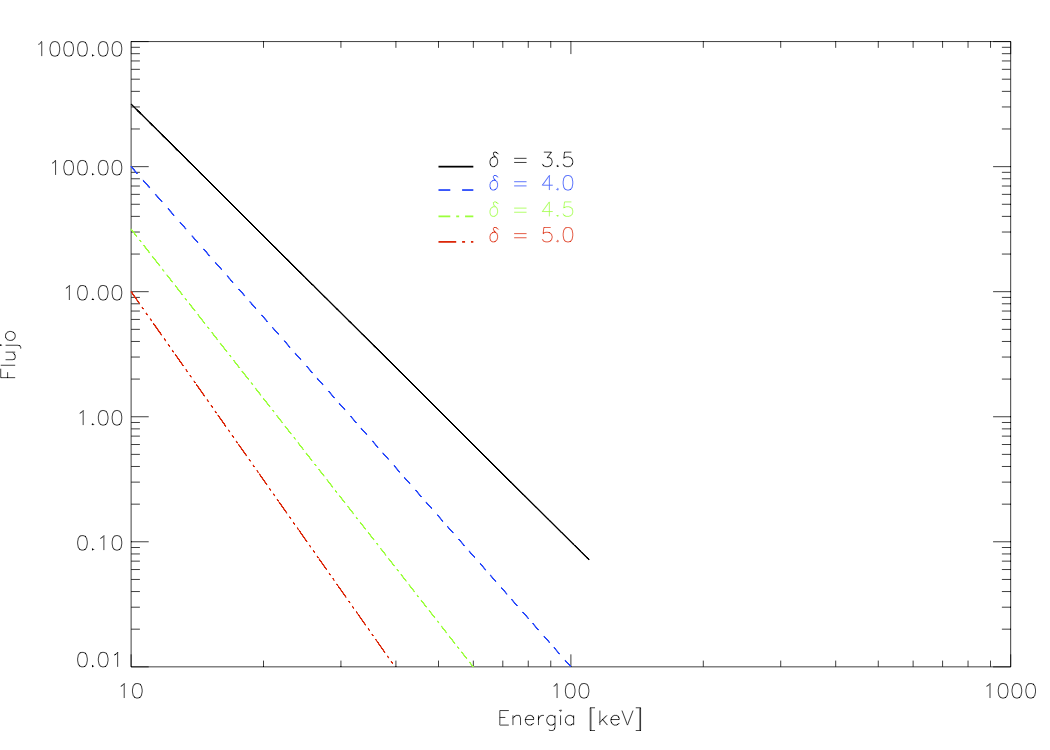
\includegraphics[width=0.39\textwidth]{delta.png}
\caption{Ejemplo de las distribuciones tipo ley de potencias usadas para ajustar la parte de emisi\'on no-t\'ermica de un espectro t\'ipico de una fulguraci\'on solar con una emisi\'on discernible en rayos-X duros. Como se ejemplifica en el cuadro \ref{table:kontar} los \'indices $\delta$ usualmente toman valores entre 3.5 y 5.0. Para la distribuci\'on energ\'etica de la distribuci\'on de densidad electr\'onica que se introduce como {\it input} en nuestra simulaci\'on usamos valores para $\delta$ en el rango que se muestra aqu\'i.}
\label{fig:delta}
\end{center}
\end{wrapfigure}

Por otro lado, si se asume que la funci\'on de distribuci\'on de densidad electr\'onica obedece tambi\'en una ley de potencias, es decir $f_{\text{electrones}}\propto E^{-\delta}$, el \'indice de la ley de potencia $\delta$ debe estar relacionado de alguna manera con el \'indice espectral $\gamma$. As\'i, dependiendo del tipo de interacci\'on entre los electrones acelerados y el plasma del ambiente circundante a la posici\'on donde la emisi\'on fot\'onica tiene lugar, esta relaci\'on toma una forma que depende esencialmente del mecanismo dominante de radiaci\'on. \cite{Tandberg-Hanssen1988} hacen una descripci\'on de este tipo de relaci\'on entre los dos \'indices a trav\'es de los dos modelos que han demostrado mayor \'exito hasta el momento en su contraste con los resultados observacionales, el llamado modelo de {\bf blanco grueso} ({\it thick target model}) y el modelo de {\bf blanco delgado} ({\it thin target model}). Seg\'un estos modelos, esta relaci\'on est\'a dada por

\begin{align}
\gamma_{thin}=\delta + 0.5\qquad\gamma_{thick}=\delta - 1.5\text{.}
\end{align}

La realidad es que el valor num\'erico de estos \'indices de deben encontrar de forma emp\'irica. Muchos trabajos en torno al mejor ajuste de los espectros observacionales de diferentes fulguraciones han sido desarrollados, obteniendo rangos de validez para estos \'indices entre $2\lesssim\delta\lesssim8$ y $3\lesssim\gamma\lesssim9$ \citep{grigis2006}. Un ejemplo de este tipo de an\'alisis observacional lo muestran \cite{kontar2002}, quienes para cuatro eventos de fulguraciones altamente energ\'eticas reportan valores de \'indice espectral de los electrones como se puede apreciar en el cuadro \ref{table:kontar}.

\begin{table}
\centering
\begin{tabular}{ l c c }\hline
Fecha & Hora (TU) & $\delta$ \\\hline
  20 Feb 2002 & 11:06:00 - 11:06:40 & 4.89 \\
  17 Mar 2002 & 19:27:30 - 19:29:10 & 4.84 \\
  31 May 2002 & 00:06:40 - 00:08:00 & 3.79 \\
  01 Jun 2002 & 03:53:10 - 03:54:30 & 4.26 \\\hline
\end{tabular}
\caption{\'Indice de la ley de potencias que obedece la distribuci\'on de densidad de electrones para cuatro fulguraciones diferentes que tuvieron lugar en 2002. El valor de cada \'indice se determin\'o usando un blanco ionizado uniforme bajo el protocolo usado por defecto por SPEX, el software especializado de RHESSI para estos menesteres \cite[]{kontar2002}.}
\label{table:kontar}
\end{table}

Teniendo en cuenta lo anterior, no estamos muy lejos de la realidad f\'isica si para el tiempo inicial imponemos que la distribuci\'on de densidad electr\'onica en funci\'on de la energ\'ia obedecer\'a una ley de potencia con \'indice $\delta=4.5$. En general, 

\begin{align}
f_{\text{electrones}}=A_e(m_ec^2)^{-\delta}
\end{align}

\noindent donde $A_e$ es una constante de ajuste al espectro seg\'un el flujo que se tenga y $m_ec^2$ es la energ\'ia total de un electr\'on t\'ipico (la suma de la energ\'ia en reposo m\'as su energ\'ia cin\'etica).\\

\begin{wrapfigure}[31]{r}{0.5\textwidth}
\begin{center}
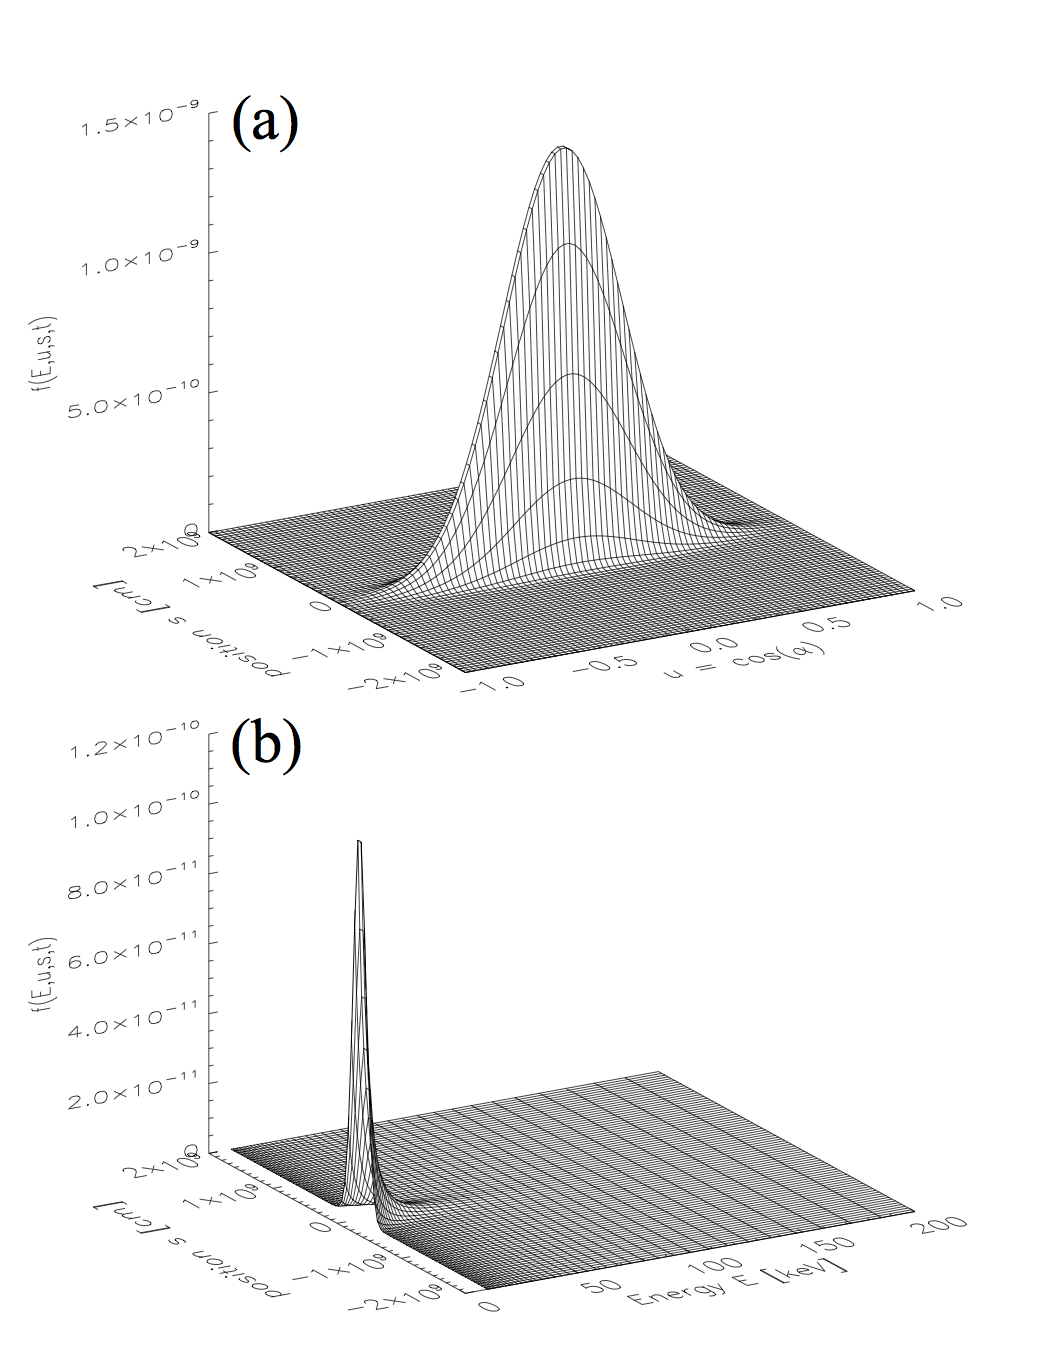
\includegraphics[width=0.5\textwidth]{input.png}
\caption{Funci\'on de entrada para la distribuci\'on de densidad de probabilidad electr\'onica. {\bf (a)} Dependencia gaussiana con la posici\'on y el \'angulo de inclinaci\'on. {\bf (b)} Dependencia con la posici\'on y la energ\'ia.}
\label{fig:input}
\end{center}
\end{wrapfigure}

Siguiendo con la discusi\'on de c\'omo debe ser la distribuci\'on inicial del programa que resuelve num\'ericamente la ecuaci\'on de {\it Fokker-Planck} en funci\'on de cada una de las variables de las que depende, ahora es el turno de discutir la distribuci\'on inicial de la densidad electr\'onica en funci\'on del \'angulo de inclinaci\'on $\alpha$, o equivalentemente del coseno de este, $\mu=\cos\alpha$. Una vez el {\it jet} de part\'iculas es inyectado en el bucle solar por la cima de este, la direcci\'on en la que inciden cada una de ellas tiene un sentido preferencial que resulta ser perpendicular a las l\'ineas de campo magn\'etico en esa localidad, es decir $\cos\alpha=0$. Este proceso de inyecci\'on est\'a acompa\~nado de varios fen\'omenos aleatorios, la distribuci\'on incidente se debe poder modelar como una distribuci\'on gaussiana con cierto valor de desviaci\'on est\'andar. As\'i, $f_\alpha = A_\alpha\exp\left[-\frac{\mu^2}{2\,d\mu^2}\right]$, siendo $A_\alpha$ una constante de normalizaci\'on o de ajuste y $d\mu$ la desviaci\'on est\'andar. Algunos trabajos se han desarrollado tratando de describir la mejor funci\'on de distribuci\'on en funci\'on del \'angulo de inclinaci\'on que mejor se acomode a los resultados observacionales y que pueda ser usada como par\'ametro de entrada en los diferentes c\'odigos num\'ericos relacionados con este fen\'omeno. Siguiendo a \cite{2000leegary} nosotros usamos para $t=0$, los valores iniciales $\mu=0$ para el coseno del \'angulo de inclinaci\'on $\alpha$ y $d\mu=0.26$ para su desviaci\'on est\'andar respectivamente.\\

Usamos tambi\'en una distribuci\'on con dependencia gaussiana en la posici\'on, esto es

\begin{align}
f_s = A_s\exp\left[-\frac{s^2}{2\,ds^2}\right],
\end{align}

\noindent con $ds=10^{8}$ cm (dos \'ordenes de magnitud menor que la longitud t\'ipica de un bucle solar), en donde $ds$ es la desviaci\'on est\'andar respectiva. De esta manera, la distribuci\'on de densidad de probabilidad en funci\'on de la posici\'on, el \'angulo de inclinaci\'on y de la posici\'on para el momento de la inyecci\'on (que usamos como par\'ametro de entrada de nuestra simulaci\'on) es algo como lo que se muestra en a figura \ref{fig:input}.\\

Es importante precisar tambi\'en la forma temporal en la que deben ser inyectadas las part\'iculas en la cima del bucle. Num\'ericamente lo m\'as sencillo es hacer que todo el conjunto de part\'iculas aparezcan en la cima s\'ubitamente para un tiempo dado (el tiempo inicial) tal y como funciona el c\'odio original desarrollado por \cite{hamilton1990}. Sin embargo, esto no es del todo cierto durante el fen\'omeno f\'isico real; en el momento de la inyecci\'on las part\'iculas arriban al bucle con cierta distribuci\'on temporal. Siguiendo a \cite{aschwanden2004}, este tiempo de inyecci\'on de las part\'iculas es m\'as importante que el tiempo en el cual se hayan acelerado las part\'iculas, previas a su incidencia sobre la cima del bucle, para determinar la escala de tiempo de emisi\'on en rayos-X duros, y lo cual es lo que nos caracteriza la din\'amica del proceso post-reconexi\'on.\\

Una vez definida la f\'isica detr\'as de la inyecci\'on del conjunto de electrones acelerados en la cima de bucle solar podemos centrarnos m\'as en los detalles t\'ecnicos relacionados con los par\'ametros iniciales que se deben suministrar al conjunto de programas que resuelve la ecuaci\'on de {\it Fokker-Planck} dependiente del tiempo que es justamente el tema que abordamos a continuaci\'on.





%Hacer gr�fica de alpha vs. t .... como son variables linealmente independientes esta dependencia da una l�nea reca creciente.

%introducir alpha=0 a ver que pasa

% Pilas con esto para las conclusiones y la variaci�n de la corrida del programa: AshwandenLa duraci\'on del pulso visto en rayos-X duros es controlada principalmente por el tiempo de inyecci\'on m\'as que la escala de tiempo de la aceleraci�n. Esto quiere decir que es vitalmente importante el tiempo de inyecci�n de las part�culas. 


\subsection*{Par\'ametros de entrada del conjunto de programas}
\addcontentsline{toc}{subsection}{Par\'ametros de entrada del conjunto de programas}


\begin{wrapfigure}[25]{l}{0.46\textwidth}
\begin{center}
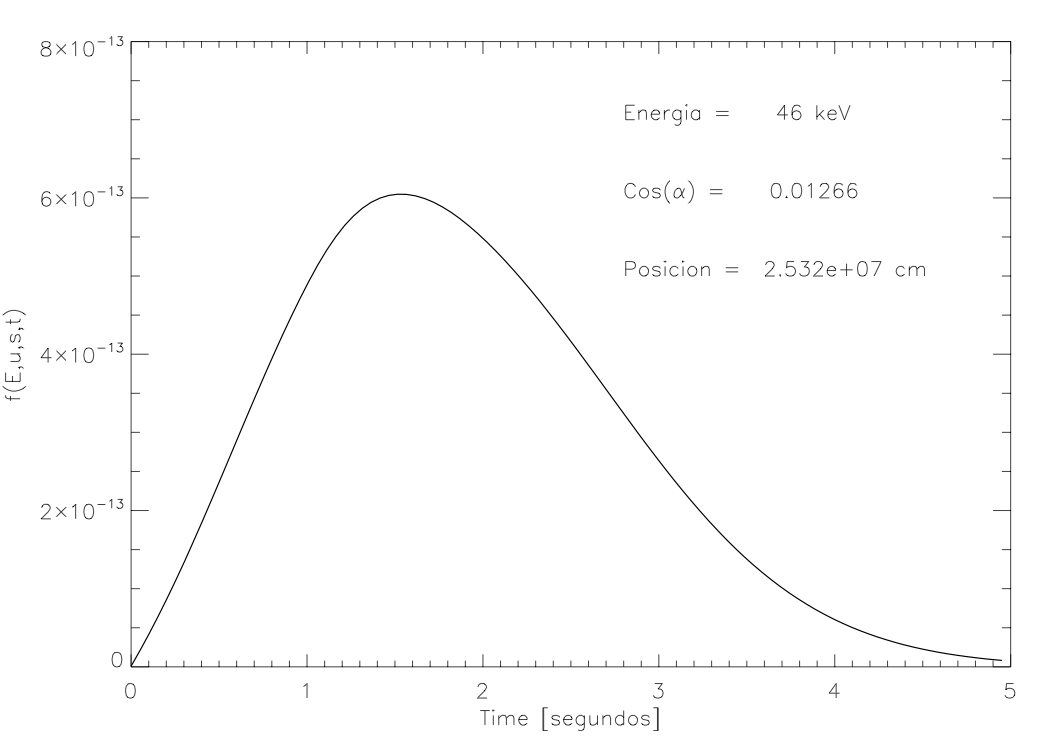
\includegraphics[width=0.44\textwidth]{image_ft.png}
\caption{Evoluci\'on temporal de la distribuci\'on de densidad de probabilidad electr\'onica usado en la simulaci\'on con una energ\'ia de 46 keV, una \'angulo de inclinaci\'on de $89.3^\circ$ y una posici\'on fija de $2.532\times10^{7}$ cm. Se ve claramente que la funci\'on de inyecci\'on de part\'iculas obedece una forma gaussiana y que la intensidad m\'axima de inyecci\'on se alcanza cerca de $\sim 1$ segundo como propone \cite{aschwanden2004}.}
\label{fig:tf}
\end{center}
\end{wrapfigure}

Definir el tama\~no de la grilla:  {\bf ned} es la cantidad de pasos en energ\'ia (por defecto usamos 40), {\bf nud} es la cantidad de pasos en el \'angulo de inclinaci\'on (por defecto usamos 80), {\bf nsd} es la cantidad de pasos en la longitud del bucle (por defecto usamos 80), {\bf ntd} es la cantidad de pasos en tiempo (por defecto usamos 100). Se definen los l\'imites en energ\'ia en keV, as\'i  {\bf emin}  define el l\'imite inferior (por defecto usamos 10), {\bf emax} define el l\'imite superior (por defecto usamos 200). Definimos los l\'imites en la posici\'on a lo largo del bucle, as\'i {\bf smin} define el l\'imite inferior en la longitud del bucle (usualmente usamos $-2\times10^9$ m) y {\bf smax} define el l\'imite superior en la longitud del bucle (usualmente usamos $2\times10^9$ m). La simulaci\'on debe contener un modelo de distribuci\'on de campo magn\'etico a lo largo del bucle, este puede ser un modelo parab\'olico dado por la expresi\'on $B(s)=B_0\times(1+s^n/LB^n)$ o un modelo exponencial dado por la ecuaci\'on $B(s) = \exp\left(\log(mr)\frac{s}{l}^n\right)$. de manera que es necesario definir la {\it raz\'on de reflejo magn\'etico} {\bf mr}$=\frac{B(s)}{B_0}$ (por defecto lo tomamos como 2); {\bf nexp} que es el exponente que va en las expresiones para el calculo del campo magn\'etico a lo largo del bucle, entre mayor sea este n\'umero mayor es el confinamiento de las part\'iculas en los pies del bucle, pero un modelo parab\'olico exige $nexp=2$. Como hay dos modelos de campo magn\'etico, al programa le indicamos cu\'al de los dos queremos usar a trav\'es de la variable {\bf bmodel} que si es cero tomar\'a el modelpo parab\'olicpo, y si en uno tomar\'a el modelo exponencial. Adem\'as se debe definir la densidad de n\'umero de part\'iculas del plasma, esto se hace a trav\'es de {\bf nmin} y {\bf nmax} (son valores alrededor de $10^{10}$ cm$^-3$). El tiempo de la simulaci\'on est\'a en segundos y es el tiempo fenomenol\'ogico  del proceso que se est\'a simulando, {\bf tmax} (tipicamente igual a 5 segundos). Por \'ultimo, debemos definir la funci\'on de distribuci\'on de las part\'iculas que se inyectan. Dicha funci\'on debe definir la distribuci\'on de la energ\'ia, el \'angulo de inclinaci\'on y la distancia a lo largo del bucle para el conjunto de part\'iculas inyectadas. Esto se hace mediante un par de distribuciones gaussianas en el \'angulo de inclinaci\'on y en la distancia a lo largo del bucle, $f_\alpha = A_\alpha\exp\left[-\frac{p^2}{2\,dp^2}\right]$ y $f_s=A_s\exp\left[-\frac{x^2}{2\,dx^2}\right]$ respectivamente. La distribuci\'on de energ\'ia de las part\'iculas en una ley de potencias de la forma $fe=A_e(mc^2)^{-\delta}$. As\'i debemos definir las variables {\bf d0}$=\delta$ que es el \'indice de la ley de potencias inicial para la energ\'ia del conjunto de part\'iculas (usualmente 4.5). {\bf dp} es la desviaci\'on est\'andar para la distribuci\'on del \'angulo de inclinaci\'on (por defecto escogemos 0.26). {\bf p0} es el centro de la ditribuci\'on gaussiana definida para el \'angulo de inclinaci\'on (comunmente se toma p0=0 porque se trata del coseno del \'angulo de inclinaci\'on, y esto significa $\alpha=90^\circ$). De manera similar {\bf xd} es la desviaci\'on est\'andar en la distribuci\'on gaussiana inicial propuesta para la variable espacial (debe estar alrededor de un ord\'en de magnitud menor a la longitud total del bucle), y {\bf x0} es el centro de la distribuci\'on espacial (por defecto se toma como cero, a menos que se quiera una mayor distribuci\'on sobre alguna de las patas del bucle). {\bf t0} es el tiempo posterior a la reconexi\'on donde ocurre el m\'aximo en la distribuci\'on de part\'iculas (comunmente se toma como $1.0$ segundo). Finalmente {\bf tau} es la desviaci\'on est\'andar en tiempo para la distribuci\'on inicial de las part\'iculas (por defecto se toma igual a $2.0$). Si se quiere inyectar un pulso repentino de part\'iculas en un mismo punto, se debe tomar tau = 0. Adem\'as de esto el conjunto de programas est\'a en la capacidad de considerar varios procesos f\'isicos asociados con el fen\'omeno de la aceleraci\'on estoc\'astica de part\'iculas en un bucle solar. Para poder hacer cambios en los c\'odigos de una manera m\'a c\'omodo, y en busca de hacer un seguimiento de la forma en que cada uno de estos procesos afecta la din\'amica del conjunto completo de part\'iculas, se han introducido las variables {\bf run0}, {\bf run1}, {\bf run2}, {\bf run3} y {\bf run4}. Cada una de est\'as puede tomar uno de dos \'unicos valores, {\bf 1} si se va a considerar como activo en el momento de de ejcutar el programa o {\bf 0} si no se considera. {\bf run 0} activa el transporte (movimiento a lo largo del bucle solar) de todas las part\'iculas. {\bf run1} activa la capacidad de las part\'iculas de perder energ\'ia a trav\'es de lo diferentes procesos que se mencionaron e el capitulo anterior. {\bf run2} activa  la reflexi\'on magn\'etica en el bu\'cle, que como ya se vi\'o depende del {\it \'angulo de inclinaci\'on} y la magnitud del campo magn\'etico. {\bf run3} activa la difusi\'on Coulmbiana de las part\'iculas aceleradas cuando interact\'uan con el plasma ambiental. {\bf run4} define un tiempo finito de inyecci\'on de las part\'iculas a acelerar dentro del bucle.\\



Una vez definidos todos estos par\'ametros, procedemos a correr el conjunto de c\'odigos con los valores de cada variable inicial como se indic\'o en el p\'arrafo anterior con el objetivo principal de hacer una primera prueba de calibraci\'on y de referencia del funcionamiento b\'asico de la simulaci\'on. 







%\input{tipos_aceleracion.tex}
%\inpu{motivacion_fpecuacion.tex}
%\input{luz_blanca_sunquakes.tex}
%\input{modelo_ashwanden.tex}
%\input{simulacion.tex}
%\input{discusion.tex}
\selectbiblanguage{spanish}
\bibliographystyle{apalike}
\bibliography{MyLibrary}
\end{document}

